\documentclass[twoside]{book}

% Packages required by doxygen
\usepackage{fixltx2e}
\usepackage{calc}
\usepackage{doxygen}
\usepackage{graphicx}
\usepackage[utf8]{inputenc}
\usepackage{makeidx}
\usepackage{multicol}
\usepackage{multirow}
\PassOptionsToPackage{warn}{textcomp}
\usepackage{textcomp}
\usepackage[nointegrals]{wasysym}
\usepackage[table]{xcolor}
\usepackage{ifpdf,ifxetex}

% Font selection
\usepackage[T1]{fontenc}
\usepackage[scaled=.90]{helvet}
\usepackage{courier}
\usepackage{amssymb}
\usepackage{sectsty}
\renewcommand{\familydefault}{\sfdefault}
\allsectionsfont{%
  \fontseries{bc}\selectfont%
  \color{darkgray}%
}
\renewcommand{\DoxyLabelFont}{%
  \fontseries{bc}\selectfont%
  \color{darkgray}%
}
\newcommand{\+}{\discretionary{\mbox{\scriptsize$\hookleftarrow$}}{}{}}

% Page & text layout
\usepackage{geometry}
\geometry{%
  a4paper,%
  top=2.5cm,%
  bottom=2.5cm,%
  left=2.5cm,%
  right=2.5cm%
}
\tolerance=750
\hfuzz=15pt
\hbadness=750
\setlength{\emergencystretch}{15pt}
\setlength{\parindent}{0cm}
\setlength{\parskip}{3ex plus 2ex minus 2ex}
\makeatletter
\renewcommand{\paragraph}{%
  \@startsection{paragraph}{4}{0ex}{-1.0ex}{1.0ex}{%
    \normalfont\normalsize\bfseries\SS@parafont%
  }%
}
\renewcommand{\subparagraph}{%
  \@startsection{subparagraph}{5}{0ex}{-1.0ex}{1.0ex}{%
    \normalfont\normalsize\bfseries\SS@subparafont%
  }%
}
\makeatother

% Headers & footers
\usepackage{fancyhdr}
\pagestyle{fancyplain}
\fancyhead[LE]{\fancyplain{}{\bfseries\thepage}}
\fancyhead[CE]{\fancyplain{}{}}
\fancyhead[RE]{\fancyplain{}{\bfseries\leftmark}}
\fancyhead[LO]{\fancyplain{}{\bfseries\rightmark}}
\fancyhead[CO]{\fancyplain{}{}}
\fancyhead[RO]{\fancyplain{}{\bfseries\thepage}}
\fancyfoot[LE]{\fancyplain{}{}}
\fancyfoot[CE]{\fancyplain{}{}}
\fancyfoot[RE]{\fancyplain{}{\bfseries\scriptsize Generated by Doxygen }}
\fancyfoot[LO]{\fancyplain{}{\bfseries\scriptsize Generated by Doxygen }}
\fancyfoot[CO]{\fancyplain{}{}}
\fancyfoot[RO]{\fancyplain{}{}}
\renewcommand{\footrulewidth}{0.4pt}
\renewcommand{\chaptermark}[1]{%
  \markboth{#1}{}%
}
\renewcommand{\sectionmark}[1]{%
  \markright{\thesection\ #1}%
}

% Indices & bibliography
\usepackage{natbib}
\usepackage[titles]{tocloft}
\setcounter{tocdepth}{3}
\setcounter{secnumdepth}{5}
\makeindex

% Hyperlinks (required, but should be loaded last)
\ifpdf
  \usepackage[pdftex,pagebackref=true]{hyperref}
\else
  \ifxetex
    \usepackage[pagebackref=true]{hyperref}
  \else
    \usepackage[ps2pdf,pagebackref=true]{hyperref}
  \fi
\fi
\ifpdf
  \DeclareUnicodeCharacter{207B}{${}^{-}$}% Superscript minus
  \DeclareUnicodeCharacter{C2B2}{${}^{2}$}% Superscript two
  \DeclareUnicodeCharacter{C2B3}{${}^{3}$}% Superscript three
\else
  \catcode`\⁻=13% Superscript minus
  \def⁻{${}^{-}$}
  \catcode`\²=13% Superscript two
  \def²{${}^{2}$}
  \catcode`\³=13% Superscript three
  \def³{${}^{3}$}
\fi

\hypersetup{%
  colorlinks=true,%
  linkcolor=blue,%
  citecolor=blue,%
  unicode%
}

% Custom commands
\newcommand{\clearemptydoublepage}{%
  \newpage{\pagestyle{empty}\cleardoublepage}%
}

\usepackage{caption}
\captionsetup{labelsep=space,justification=centering,font={bf},singlelinecheck=off,skip=4pt,position=top}

\renewcommand{\numberline}[1]{#1~}
%===== C O N T E N T S =====

\begin{document}

% Titlepage & ToC
\hypersetup{pageanchor=false,
             bookmarksnumbered=true,
             pdfencoding=unicode
            }
\pagenumbering{alph}
\begin{titlepage}
\vspace*{7cm}
\begin{center}%
{\Large jaegertracingc }\\
\vspace*{1cm}
{\large Generated by Doxygen 1.8.15}\\
\end{center}
\end{titlepage}
\clearemptydoublepage
\pagenumbering{roman}
\tableofcontents
\clearemptydoublepage
\pagenumbering{arabic}
\hypersetup{pageanchor=true}

%--- Begin generated contents ---
\chapter{Hierarchical Index}
\section{Class Hierarchy}
This inheritance list is sorted roughly, but not completely, alphabetically\+:\begin{DoxyCompactList}
\item \contentsline{section}{\+\_\+\+Jaegertracing\+\_\+\+\_\+\+Protobuf\+\_\+\+\_\+\+Agent\+\_\+\+\_\+\+Agent\+\_\+\+Service}{\pageref{struct__Jaegertracing____Protobuf____Agent____Agent__Service}}{}
\item \contentsline{section}{\+\_\+\+Jaegertracing\+\_\+\+\_\+\+Protobuf\+\_\+\+\_\+\+Agent\+\_\+\+\_\+\+Empty}{\pageref{struct__Jaegertracing____Protobuf____Agent____Empty}}{}
\item \contentsline{section}{\+\_\+\+Jaegertracing\+\_\+\+\_\+\+Protobuf\+\_\+\+\_\+\+Baggage\+\_\+\+\_\+\+Baggage\+Restriction}{\pageref{struct__Jaegertracing____Protobuf____Baggage____BaggageRestriction}}{}
\item \contentsline{section}{\+\_\+\+Jaegertracing\+\_\+\+\_\+\+Protobuf\+\_\+\+\_\+\+Baggage\+\_\+\+\_\+\+Baggage\+Restriction\+Manager\+\_\+\+Service}{\pageref{struct__Jaegertracing____Protobuf____Baggage____BaggageRestrictionManager__Service}}{}
\item \contentsline{section}{\+\_\+\+Jaegertracing\+\_\+\+\_\+\+Protobuf\+\_\+\+\_\+\+Baggage\+\_\+\+\_\+\+Baggage\+Restriction\+Request}{\pageref{struct__Jaegertracing____Protobuf____Baggage____BaggageRestrictionRequest}}{}
\item \contentsline{section}{\+\_\+\+Jaegertracing\+\_\+\+\_\+\+Protobuf\+\_\+\+\_\+\+Baggage\+\_\+\+\_\+\+Baggage\+Restriction\+Response}{\pageref{struct__Jaegertracing____Protobuf____Baggage____BaggageRestrictionResponse}}{}
\item \contentsline{section}{\+\_\+\+Jaegertracing\+\_\+\+\_\+\+Protobuf\+\_\+\+\_\+\+Batch}{\pageref{struct__Jaegertracing____Protobuf____Batch}}{}
\item \contentsline{section}{\+\_\+\+Jaegertracing\+\_\+\+\_\+\+Protobuf\+\_\+\+\_\+\+Batch\+Response}{\pageref{struct__Jaegertracing____Protobuf____BatchResponse}}{}
\item \contentsline{section}{\+\_\+\+Jaegertracing\+\_\+\+\_\+\+Protobuf\+\_\+\+\_\+\+Collector\+\_\+\+Service}{\pageref{struct__Jaegertracing____Protobuf____Collector__Service}}{}
\item \contentsline{section}{\+\_\+\+Jaegertracing\+\_\+\+\_\+\+Protobuf\+\_\+\+\_\+\+Log}{\pageref{struct__Jaegertracing____Protobuf____Log}}{}
\item \contentsline{section}{\+\_\+\+Jaegertracing\+\_\+\+\_\+\+Protobuf\+\_\+\+\_\+\+Process}{\pageref{struct__Jaegertracing____Protobuf____Process}}{}
\item \contentsline{section}{\+\_\+\+Jaegertracing\+\_\+\+\_\+\+Protobuf\+\_\+\+\_\+\+Sampling\+Manager\+\_\+\+\_\+\+Per\+Operation\+Sampling\+Strategy}{\pageref{struct__Jaegertracing____Protobuf____SamplingManager____PerOperationSamplingStrategy}}{}
\item \contentsline{section}{\+\_\+\+Jaegertracing\+\_\+\+\_\+\+Protobuf\+\_\+\+\_\+\+Sampling\+Manager\+\_\+\+\_\+\+Per\+Operation\+Sampling\+Strategy\+\_\+\+\_\+\+Operation\+Sampling\+Strategy}{\pageref{struct__Jaegertracing____Protobuf____SamplingManager____PerOperationSamplingStrategy____OperationSamplingStrategy}}{}
\item \contentsline{section}{\+\_\+\+Jaegertracing\+\_\+\+\_\+\+Protobuf\+\_\+\+\_\+\+Sampling\+Manager\+\_\+\+\_\+\+Probabilistic\+Sampling\+Strategy}{\pageref{struct__Jaegertracing____Protobuf____SamplingManager____ProbabilisticSamplingStrategy}}{}
\item \contentsline{section}{\+\_\+\+Jaegertracing\+\_\+\+\_\+\+Protobuf\+\_\+\+\_\+\+Sampling\+Manager\+\_\+\+\_\+\+Rate\+Limiting\+Sampling\+Strategy}{\pageref{struct__Jaegertracing____Protobuf____SamplingManager____RateLimitingSamplingStrategy}}{}
\item \contentsline{section}{\+\_\+\+Jaegertracing\+\_\+\+\_\+\+Protobuf\+\_\+\+\_\+\+Sampling\+Manager\+\_\+\+\_\+\+Sampling\+Manager\+\_\+\+Service}{\pageref{struct__Jaegertracing____Protobuf____SamplingManager____SamplingManager__Service}}{}
\item \contentsline{section}{\+\_\+\+Jaegertracing\+\_\+\+\_\+\+Protobuf\+\_\+\+\_\+\+Sampling\+Manager\+\_\+\+\_\+\+Sampling\+Strategy\+Request}{\pageref{struct__Jaegertracing____Protobuf____SamplingManager____SamplingStrategyRequest}}{}
\item \contentsline{section}{\+\_\+\+Jaegertracing\+\_\+\+\_\+\+Protobuf\+\_\+\+\_\+\+Sampling\+Manager\+\_\+\+\_\+\+Sampling\+Strategy\+Response}{\pageref{struct__Jaegertracing____Protobuf____SamplingManager____SamplingStrategyResponse}}{}
\item \contentsline{section}{\+\_\+\+Jaegertracing\+\_\+\+\_\+\+Protobuf\+\_\+\+\_\+\+Span}{\pageref{struct__Jaegertracing____Protobuf____Span}}{}
\item \contentsline{section}{\+\_\+\+Jaegertracing\+\_\+\+\_\+\+Protobuf\+\_\+\+\_\+\+Span\+Ref}{\pageref{struct__Jaegertracing____Protobuf____SpanRef}}{}
\item \contentsline{section}{\+\_\+\+Jaegertracing\+\_\+\+\_\+\+Protobuf\+\_\+\+\_\+\+Tag}{\pageref{struct__Jaegertracing____Protobuf____Tag}}{}
\item \contentsline{section}{\+\_\+\+Jaegertracing\+\_\+\+\_\+\+Protobuf\+\_\+\+\_\+\+Trace\+ID}{\pageref{struct__Jaegertracing____Protobuf____TraceID}}{}
\item \contentsline{section}{extract\+\_\+text\+\_\+map\+\_\+arg}{\pageref{structextract__text__map__arg}}{}
\item \contentsline{section}{jaeger\+\_\+adaptive\+\_\+sampler}{\pageref{structjaeger__adaptive__sampler}}{}
\item \contentsline{section}{jaeger\+\_\+allocator}{\pageref{structjaeger__allocator}}{}
\item \contentsline{section}{jaeger\+\_\+baggage\+\_\+restriction}{\pageref{structjaeger__baggage__restriction}}{}
\item \contentsline{section}{jaeger\+\_\+baggage\+\_\+restriction\+\_\+manager}{\pageref{structjaeger__baggage__restriction__manager}}{}
\begin{DoxyCompactList}
\item \contentsline{section}{jaeger\+\_\+default\+\_\+baggage\+\_\+restriction\+\_\+manager}{\pageref{structjaeger__default__baggage__restriction__manager}}{}
\end{DoxyCompactList}
\item \contentsline{section}{jaeger\+\_\+baggage\+\_\+restrictions\+\_\+config}{\pageref{structjaeger__baggage__restrictions__config}}{}
\item \contentsline{section}{jaeger\+\_\+baggage\+\_\+setter}{\pageref{structjaeger__baggage__setter}}{}
\item \contentsline{section}{jaeger\+\_\+composite\+\_\+reporter}{\pageref{structjaeger__composite__reporter}}{}
\item \contentsline{section}{jaeger\+\_\+config}{\pageref{structjaeger__config}}{}
\item \contentsline{section}{jaeger\+\_\+const\+\_\+sampler}{\pageref{structjaeger__const__sampler}}{}
\item \contentsline{section}{jaeger\+\_\+default\+\_\+counter}{\pageref{structjaeger__default__counter}}{}
\item \contentsline{section}{jaeger\+\_\+default\+\_\+gauge}{\pageref{structjaeger__default__gauge}}{}
\item jaeger\+\_\+destructible\begin{DoxyCompactList}
\item \contentsline{section}{jaeger\+\_\+counter}{\pageref{structjaeger__counter}}{}
\item \contentsline{section}{jaeger\+\_\+gauge}{\pageref{structjaeger__gauge}}{}
\item \contentsline{section}{jaeger\+\_\+list\+\_\+node}{\pageref{structjaeger__list__node}}{}
\end{DoxyCompactList}
\item \contentsline{section}{jaeger\+\_\+guaranteed\+\_\+throughput\+\_\+probabilistic\+\_\+sampler}{\pageref{structjaeger__guaranteed__throughput__probabilistic__sampler}}{}
\item \contentsline{section}{jaeger\+\_\+hashtable}{\pageref{structjaeger__hashtable}}{}
\item \contentsline{section}{jaeger\+\_\+hashtable\+\_\+lookup\+\_\+result}{\pageref{structjaeger__hashtable__lookup__result}}{}
\item \contentsline{section}{jaeger\+\_\+headers\+\_\+config}{\pageref{structjaeger__headers__config}}{}
\item \contentsline{section}{jaeger\+\_\+host\+\_\+port}{\pageref{structjaeger__host__port}}{}
\item \contentsline{section}{jaeger\+\_\+http\+\_\+sampling\+\_\+manager}{\pageref{structjaeger__http__sampling__manager}}{}
\item \contentsline{section}{jaeger\+\_\+in\+\_\+memory\+\_\+reporter}{\pageref{structjaeger__in__memory__reporter}}{}
\item \contentsline{section}{jaeger\+\_\+key\+\_\+value}{\pageref{structjaeger__key__value}}{}
\item \contentsline{section}{jaeger\+\_\+key\+\_\+value\+\_\+node}{\pageref{structjaeger__key__value__node}}{}
\item \contentsline{section}{jaeger\+\_\+list}{\pageref{structjaeger__list}}{}
\item \contentsline{section}{jaeger\+\_\+log\+\_\+record}{\pageref{structjaeger__log__record}}{}
\item \contentsline{section}{jaeger\+\_\+logger}{\pageref{structjaeger__logger}}{}
\item \contentsline{section}{jaeger\+\_\+metrics}{\pageref{structjaeger__metrics}}{}
\item \contentsline{section}{jaeger\+\_\+operation\+\_\+sampler}{\pageref{structjaeger__operation__sampler}}{}
\item \contentsline{section}{jaeger\+\_\+probabilistic\+\_\+sampler}{\pageref{structjaeger__probabilistic__sampler}}{}
\item \contentsline{section}{jaeger\+\_\+rate\+\_\+limiting\+\_\+sampler}{\pageref{structjaeger__rate__limiting__sampler}}{}
\item \contentsline{section}{jaeger\+\_\+remote\+\_\+reporter}{\pageref{structjaeger__remote__reporter}}{}
\item \contentsline{section}{jaeger\+\_\+remotely\+\_\+controlled\+\_\+sampler}{\pageref{structjaeger__remotely__controlled__sampler}}{}
\item \contentsline{section}{jaeger\+\_\+reporter}{\pageref{structjaeger__reporter}}{}
\item \contentsline{section}{jaeger\+\_\+reporter\+\_\+config}{\pageref{structjaeger__reporter__config}}{}
\item \contentsline{section}{jaeger\+\_\+rng}{\pageref{structjaeger__rng}}{}
\item \contentsline{section}{jaeger\+\_\+sampler}{\pageref{structjaeger__sampler}}{}
\item \contentsline{section}{jaeger\+\_\+sampler\+\_\+choice}{\pageref{structjaeger__sampler__choice}}{}
\item \contentsline{section}{jaeger\+\_\+sampler\+\_\+config}{\pageref{structjaeger__sampler__config}}{}
\item \contentsline{section}{jaeger\+\_\+span}{\pageref{structjaeger__span}}{}
\item \contentsline{section}{jaeger\+\_\+span\+\_\+context}{\pageref{structjaeger__span__context}}{}
\item \contentsline{section}{jaeger\+\_\+span\+\_\+ref}{\pageref{structjaeger__span__ref}}{}
\item \contentsline{section}{jaeger\+\_\+thread\+\_\+local}{\pageref{structjaeger__thread__local}}{}
\item \contentsline{section}{jaeger\+\_\+token\+\_\+bucket}{\pageref{structjaeger__token__bucket}}{}
\item \contentsline{section}{jaeger\+\_\+trace\+\_\+id}{\pageref{structjaeger__trace__id}}{}
\item \contentsline{section}{jaeger\+\_\+tracer}{\pageref{structjaeger__tracer}}{}
\item \contentsline{section}{jaeger\+\_\+tracer\+\_\+options}{\pageref{structjaeger__tracer__options}}{}
\item \contentsline{section}{jaeger\+\_\+url}{\pageref{structjaeger__url}}{}
\item \contentsline{section}{jaeger\+\_\+vector}{\pageref{structjaeger__vector}}{}
\item \contentsline{section}{jaeger\+\_\+vector\+\_\+ptr\+\_\+copy\+\_\+arg}{\pageref{structjaeger__vector__ptr__copy__arg}}{}
\item \contentsline{section}{mock\+\_\+http\+\_\+response}{\pageref{structmock__http__response}}{}
\item \contentsline{section}{mock\+\_\+http\+\_\+server}{\pageref{structmock__http__server}}{}
\item \contentsline{section}{mock\+\_\+http\+\_\+server\+\_\+context}{\pageref{structmock__http__server__context}}{}
\item \contentsline{section}{parsing\+\_\+context}{\pageref{structparsing__context}}{}
\end{DoxyCompactList}

\chapter{Data Structure Index}
\section{Data Structures}
Here are the data structures with brief descriptions\+:\begin{DoxyCompactList}
\item\contentsline{section}{\mbox{\hyperlink{struct__Jaegertracing____Protobuf____Agent____Agent__Service}{\+\_\+\+Jaegertracing\+\_\+\+\_\+\+Protobuf\+\_\+\+\_\+\+Agent\+\_\+\+\_\+\+Agent\+\_\+\+Service}} }{\pageref{struct__Jaegertracing____Protobuf____Agent____Agent__Service}}{}
\item\contentsline{section}{\mbox{\hyperlink{struct__Jaegertracing____Protobuf____Agent____Empty}{\+\_\+\+Jaegertracing\+\_\+\+\_\+\+Protobuf\+\_\+\+\_\+\+Agent\+\_\+\+\_\+\+Empty}} }{\pageref{struct__Jaegertracing____Protobuf____Agent____Empty}}{}
\item\contentsline{section}{\mbox{\hyperlink{struct__Jaegertracing____Protobuf____Baggage____BaggageRestriction}{\+\_\+\+Jaegertracing\+\_\+\+\_\+\+Protobuf\+\_\+\+\_\+\+Baggage\+\_\+\+\_\+\+Baggage\+Restriction}} }{\pageref{struct__Jaegertracing____Protobuf____Baggage____BaggageRestriction}}{}
\item\contentsline{section}{\mbox{\hyperlink{struct__Jaegertracing____Protobuf____Baggage____BaggageRestrictionManager__Service}{\+\_\+\+Jaegertracing\+\_\+\+\_\+\+Protobuf\+\_\+\+\_\+\+Baggage\+\_\+\+\_\+\+Baggage\+Restriction\+Manager\+\_\+\+Service}} }{\pageref{struct__Jaegertracing____Protobuf____Baggage____BaggageRestrictionManager__Service}}{}
\item\contentsline{section}{\mbox{\hyperlink{struct__Jaegertracing____Protobuf____Baggage____BaggageRestrictionRequest}{\+\_\+\+Jaegertracing\+\_\+\+\_\+\+Protobuf\+\_\+\+\_\+\+Baggage\+\_\+\+\_\+\+Baggage\+Restriction\+Request}} }{\pageref{struct__Jaegertracing____Protobuf____Baggage____BaggageRestrictionRequest}}{}
\item\contentsline{section}{\mbox{\hyperlink{struct__Jaegertracing____Protobuf____Baggage____BaggageRestrictionResponse}{\+\_\+\+Jaegertracing\+\_\+\+\_\+\+Protobuf\+\_\+\+\_\+\+Baggage\+\_\+\+\_\+\+Baggage\+Restriction\+Response}} }{\pageref{struct__Jaegertracing____Protobuf____Baggage____BaggageRestrictionResponse}}{}
\item\contentsline{section}{\mbox{\hyperlink{struct__Jaegertracing____Protobuf____Batch}{\+\_\+\+Jaegertracing\+\_\+\+\_\+\+Protobuf\+\_\+\+\_\+\+Batch}} }{\pageref{struct__Jaegertracing____Protobuf____Batch}}{}
\item\contentsline{section}{\mbox{\hyperlink{struct__Jaegertracing____Protobuf____BatchResponse}{\+\_\+\+Jaegertracing\+\_\+\+\_\+\+Protobuf\+\_\+\+\_\+\+Batch\+Response}} }{\pageref{struct__Jaegertracing____Protobuf____BatchResponse}}{}
\item\contentsline{section}{\mbox{\hyperlink{struct__Jaegertracing____Protobuf____Collector__Service}{\+\_\+\+Jaegertracing\+\_\+\+\_\+\+Protobuf\+\_\+\+\_\+\+Collector\+\_\+\+Service}} }{\pageref{struct__Jaegertracing____Protobuf____Collector__Service}}{}
\item\contentsline{section}{\mbox{\hyperlink{struct__Jaegertracing____Protobuf____Log}{\+\_\+\+Jaegertracing\+\_\+\+\_\+\+Protobuf\+\_\+\+\_\+\+Log}} }{\pageref{struct__Jaegertracing____Protobuf____Log}}{}
\item\contentsline{section}{\mbox{\hyperlink{struct__Jaegertracing____Protobuf____Process}{\+\_\+\+Jaegertracing\+\_\+\+\_\+\+Protobuf\+\_\+\+\_\+\+Process}} }{\pageref{struct__Jaegertracing____Protobuf____Process}}{}
\item\contentsline{section}{\mbox{\hyperlink{struct__Jaegertracing____Protobuf____SamplingManager____PerOperationSamplingStrategy}{\+\_\+\+Jaegertracing\+\_\+\+\_\+\+Protobuf\+\_\+\+\_\+\+Sampling\+Manager\+\_\+\+\_\+\+Per\+Operation\+Sampling\+Strategy}} }{\pageref{struct__Jaegertracing____Protobuf____SamplingManager____PerOperationSamplingStrategy}}{}
\item\contentsline{section}{\mbox{\hyperlink{struct__Jaegertracing____Protobuf____SamplingManager____PerOperationSamplingStrategy____OperationSamplingStrategy}{\+\_\+\+Jaegertracing\+\_\+\+\_\+\+Protobuf\+\_\+\+\_\+\+Sampling\+Manager\+\_\+\+\_\+\+Per\+Operation\+Sampling\+Strategy\+\_\+\+\_\+\+Operation\+Sampling\+Strategy}} }{\pageref{struct__Jaegertracing____Protobuf____SamplingManager____PerOperationSamplingStrategy____OperationSamplingStrategy}}{}
\item\contentsline{section}{\mbox{\hyperlink{struct__Jaegertracing____Protobuf____SamplingManager____ProbabilisticSamplingStrategy}{\+\_\+\+Jaegertracing\+\_\+\+\_\+\+Protobuf\+\_\+\+\_\+\+Sampling\+Manager\+\_\+\+\_\+\+Probabilistic\+Sampling\+Strategy}} }{\pageref{struct__Jaegertracing____Protobuf____SamplingManager____ProbabilisticSamplingStrategy}}{}
\item\contentsline{section}{\mbox{\hyperlink{struct__Jaegertracing____Protobuf____SamplingManager____RateLimitingSamplingStrategy}{\+\_\+\+Jaegertracing\+\_\+\+\_\+\+Protobuf\+\_\+\+\_\+\+Sampling\+Manager\+\_\+\+\_\+\+Rate\+Limiting\+Sampling\+Strategy}} }{\pageref{struct__Jaegertracing____Protobuf____SamplingManager____RateLimitingSamplingStrategy}}{}
\item\contentsline{section}{\mbox{\hyperlink{struct__Jaegertracing____Protobuf____SamplingManager____SamplingManager__Service}{\+\_\+\+Jaegertracing\+\_\+\+\_\+\+Protobuf\+\_\+\+\_\+\+Sampling\+Manager\+\_\+\+\_\+\+Sampling\+Manager\+\_\+\+Service}} }{\pageref{struct__Jaegertracing____Protobuf____SamplingManager____SamplingManager__Service}}{}
\item\contentsline{section}{\mbox{\hyperlink{struct__Jaegertracing____Protobuf____SamplingManager____SamplingStrategyRequest}{\+\_\+\+Jaegertracing\+\_\+\+\_\+\+Protobuf\+\_\+\+\_\+\+Sampling\+Manager\+\_\+\+\_\+\+Sampling\+Strategy\+Request}} }{\pageref{struct__Jaegertracing____Protobuf____SamplingManager____SamplingStrategyRequest}}{}
\item\contentsline{section}{\mbox{\hyperlink{struct__Jaegertracing____Protobuf____SamplingManager____SamplingStrategyResponse}{\+\_\+\+Jaegertracing\+\_\+\+\_\+\+Protobuf\+\_\+\+\_\+\+Sampling\+Manager\+\_\+\+\_\+\+Sampling\+Strategy\+Response}} }{\pageref{struct__Jaegertracing____Protobuf____SamplingManager____SamplingStrategyResponse}}{}
\item\contentsline{section}{\mbox{\hyperlink{struct__Jaegertracing____Protobuf____Span}{\+\_\+\+Jaegertracing\+\_\+\+\_\+\+Protobuf\+\_\+\+\_\+\+Span}} }{\pageref{struct__Jaegertracing____Protobuf____Span}}{}
\item\contentsline{section}{\mbox{\hyperlink{struct__Jaegertracing____Protobuf____SpanRef}{\+\_\+\+Jaegertracing\+\_\+\+\_\+\+Protobuf\+\_\+\+\_\+\+Span\+Ref}} }{\pageref{struct__Jaegertracing____Protobuf____SpanRef}}{}
\item\contentsline{section}{\mbox{\hyperlink{struct__Jaegertracing____Protobuf____Tag}{\+\_\+\+Jaegertracing\+\_\+\+\_\+\+Protobuf\+\_\+\+\_\+\+Tag}} }{\pageref{struct__Jaegertracing____Protobuf____Tag}}{}
\item\contentsline{section}{\mbox{\hyperlink{struct__Jaegertracing____Protobuf____TraceID}{\+\_\+\+Jaegertracing\+\_\+\+\_\+\+Protobuf\+\_\+\+\_\+\+Trace\+ID}} }{\pageref{struct__Jaegertracing____Protobuf____TraceID}}{}
\item\contentsline{section}{\mbox{\hyperlink{structextract__text__map__arg}{extract\+\_\+text\+\_\+map\+\_\+arg}} }{\pageref{structextract__text__map__arg}}{}
\item\contentsline{section}{\mbox{\hyperlink{structjaeger__adaptive__sampler}{jaeger\+\_\+adaptive\+\_\+sampler}} }{\pageref{structjaeger__adaptive__sampler}}{}
\item\contentsline{section}{\mbox{\hyperlink{structjaeger__allocator}{jaeger\+\_\+allocator}} \\*Interface to override default allocator }{\pageref{structjaeger__allocator}}{}
\item\contentsline{section}{\mbox{\hyperlink{structjaeger__baggage__restriction}{jaeger\+\_\+baggage\+\_\+restriction}} \\*Representation of baggage restriction for a given key and a given service }{\pageref{structjaeger__baggage__restriction}}{}
\item\contentsline{section}{\mbox{\hyperlink{structjaeger__baggage__restriction__manager}{jaeger\+\_\+baggage\+\_\+restriction\+\_\+manager}} \\*Interface for object that manages baggage restrictions }{\pageref{structjaeger__baggage__restriction__manager}}{}
\item\contentsline{section}{\mbox{\hyperlink{structjaeger__baggage__restrictions__config}{jaeger\+\_\+baggage\+\_\+restrictions\+\_\+config}} \\*Baggage restrictions config }{\pageref{structjaeger__baggage__restrictions__config}}{}
\item\contentsline{section}{\mbox{\hyperlink{structjaeger__baggage__setter}{jaeger\+\_\+baggage\+\_\+setter}} \\*Facade to enforce remote baggage restrictions in tracer }{\pageref{structjaeger__baggage__setter}}{}
\item\contentsline{section}{\mbox{\hyperlink{structjaeger__composite__reporter}{jaeger\+\_\+composite\+\_\+reporter}} }{\pageref{structjaeger__composite__reporter}}{}
\item\contentsline{section}{\mbox{\hyperlink{structjaeger__config}{jaeger\+\_\+config}} \\*Overall Jaeger configuration object }{\pageref{structjaeger__config}}{}
\item\contentsline{section}{\mbox{\hyperlink{structjaeger__const__sampler}{jaeger\+\_\+const\+\_\+sampler}} }{\pageref{structjaeger__const__sampler}}{}
\item\contentsline{section}{\mbox{\hyperlink{structjaeger__counter}{jaeger\+\_\+counter}} \\*Counter metric interface }{\pageref{structjaeger__counter}}{}
\item\contentsline{section}{\mbox{\hyperlink{structjaeger__default__baggage__restriction__manager}{jaeger\+\_\+default\+\_\+baggage\+\_\+restriction\+\_\+manager}} \\*Default implementation of \mbox{\hyperlink{structjaeger__baggage__restriction__manager}{jaeger\+\_\+baggage\+\_\+restriction\+\_\+manager}} interface }{\pageref{structjaeger__default__baggage__restriction__manager}}{}
\item\contentsline{section}{\mbox{\hyperlink{structjaeger__default__counter}{jaeger\+\_\+default\+\_\+counter}} \\*Implements the counter interface with basic 64 bit integer value }{\pageref{structjaeger__default__counter}}{}
\item\contentsline{section}{\mbox{\hyperlink{structjaeger__default__gauge}{jaeger\+\_\+default\+\_\+gauge}} \\*Implements gauge interface with basic 64 bit integer value }{\pageref{structjaeger__default__gauge}}{}
\item\contentsline{section}{\mbox{\hyperlink{structjaeger__gauge}{jaeger\+\_\+gauge}} \\*Gauge metric interface }{\pageref{structjaeger__gauge}}{}
\item\contentsline{section}{\mbox{\hyperlink{structjaeger__guaranteed__throughput__probabilistic__sampler}{jaeger\+\_\+guaranteed\+\_\+throughput\+\_\+probabilistic\+\_\+sampler}} }{\pageref{structjaeger__guaranteed__throughput__probabilistic__sampler}}{}
\item\contentsline{section}{\mbox{\hyperlink{structjaeger__hashtable}{jaeger\+\_\+hashtable}} \\*Hashtable data structure }{\pageref{structjaeger__hashtable}}{}
\item\contentsline{section}{\mbox{\hyperlink{structjaeger__hashtable__lookup__result}{jaeger\+\_\+hashtable\+\_\+lookup\+\_\+result}} }{\pageref{structjaeger__hashtable__lookup__result}}{}
\item\contentsline{section}{\mbox{\hyperlink{structjaeger__headers__config}{jaeger\+\_\+headers\+\_\+config}} \\*H\+T\+TP headers to use for span context propagation }{\pageref{structjaeger__headers__config}}{}
\item\contentsline{section}{\mbox{\hyperlink{structjaeger__host__port}{jaeger\+\_\+host\+\_\+port}} }{\pageref{structjaeger__host__port}}{}
\item\contentsline{section}{\mbox{\hyperlink{structjaeger__http__sampling__manager}{jaeger\+\_\+http\+\_\+sampling\+\_\+manager}} }{\pageref{structjaeger__http__sampling__manager}}{}
\item\contentsline{section}{\mbox{\hyperlink{structjaeger__in__memory__reporter}{jaeger\+\_\+in\+\_\+memory\+\_\+reporter}} }{\pageref{structjaeger__in__memory__reporter}}{}
\item\contentsline{section}{\mbox{\hyperlink{structjaeger__key__value}{jaeger\+\_\+key\+\_\+value}} }{\pageref{structjaeger__key__value}}{}
\item\contentsline{section}{\mbox{\hyperlink{structjaeger__key__value__node}{jaeger\+\_\+key\+\_\+value\+\_\+node}} \\*Define link list node for key-\/value pairs }{\pageref{structjaeger__key__value__node}}{}
\item\contentsline{section}{\mbox{\hyperlink{structjaeger__list}{jaeger\+\_\+list}} \\*Linked list implementation }{\pageref{structjaeger__list}}{}
\item\contentsline{section}{\mbox{\hyperlink{structjaeger__list__node}{jaeger\+\_\+list\+\_\+node}} \\*Base class for list elements }{\pageref{structjaeger__list__node}}{}
\item\contentsline{section}{\mbox{\hyperlink{structjaeger__log__record}{jaeger\+\_\+log\+\_\+record}} }{\pageref{structjaeger__log__record}}{}
\item\contentsline{section}{\mbox{\hyperlink{structjaeger__logger}{jaeger\+\_\+logger}} \\*Logger interface to customize log output }{\pageref{structjaeger__logger}}{}
\item\contentsline{section}{\mbox{\hyperlink{structjaeger__metrics}{jaeger\+\_\+metrics}} }{\pageref{structjaeger__metrics}}{}
\item\contentsline{section}{\mbox{\hyperlink{structjaeger__operation__sampler}{jaeger\+\_\+operation\+\_\+sampler}} }{\pageref{structjaeger__operation__sampler}}{}
\item\contentsline{section}{\mbox{\hyperlink{structjaeger__probabilistic__sampler}{jaeger\+\_\+probabilistic\+\_\+sampler}} }{\pageref{structjaeger__probabilistic__sampler}}{}
\item\contentsline{section}{\mbox{\hyperlink{structjaeger__rate__limiting__sampler}{jaeger\+\_\+rate\+\_\+limiting\+\_\+sampler}} }{\pageref{structjaeger__rate__limiting__sampler}}{}
\item\contentsline{section}{\mbox{\hyperlink{structjaeger__remote__reporter}{jaeger\+\_\+remote\+\_\+reporter}} }{\pageref{structjaeger__remote__reporter}}{}
\item\contentsline{section}{\mbox{\hyperlink{structjaeger__remotely__controlled__sampler}{jaeger\+\_\+remotely\+\_\+controlled\+\_\+sampler}} }{\pageref{structjaeger__remotely__controlled__sampler}}{}
\item\contentsline{section}{\mbox{\hyperlink{structjaeger__reporter}{jaeger\+\_\+reporter}} }{\pageref{structjaeger__reporter}}{}
\item\contentsline{section}{\mbox{\hyperlink{structjaeger__reporter__config}{jaeger\+\_\+reporter\+\_\+config}} \\*Reporter config }{\pageref{structjaeger__reporter__config}}{}
\item\contentsline{section}{\mbox{\hyperlink{structjaeger__rng}{jaeger\+\_\+rng}} }{\pageref{structjaeger__rng}}{}
\item\contentsline{section}{\mbox{\hyperlink{structjaeger__sampler}{jaeger\+\_\+sampler}} }{\pageref{structjaeger__sampler}}{}
\item\contentsline{section}{\mbox{\hyperlink{structjaeger__sampler__choice}{jaeger\+\_\+sampler\+\_\+choice}} }{\pageref{structjaeger__sampler__choice}}{}
\item\contentsline{section}{\mbox{\hyperlink{structjaeger__sampler__config}{jaeger\+\_\+sampler\+\_\+config}} \\*Sampler config }{\pageref{structjaeger__sampler__config}}{}
\item\contentsline{section}{\mbox{\hyperlink{structjaeger__span}{jaeger\+\_\+span}} }{\pageref{structjaeger__span}}{}
\item\contentsline{section}{\mbox{\hyperlink{structjaeger__span__context}{jaeger\+\_\+span\+\_\+context}} \\*Span context represents propagated span identity and state }{\pageref{structjaeger__span__context}}{}
\item\contentsline{section}{\mbox{\hyperlink{structjaeger__span__ref}{jaeger\+\_\+span\+\_\+ref}} }{\pageref{structjaeger__span__ref}}{}
\item\contentsline{section}{\mbox{\hyperlink{structjaeger__thread__local}{jaeger\+\_\+thread\+\_\+local}} }{\pageref{structjaeger__thread__local}}{}
\item\contentsline{section}{\mbox{\hyperlink{structjaeger__token__bucket}{jaeger\+\_\+token\+\_\+bucket}} }{\pageref{structjaeger__token__bucket}}{}
\item\contentsline{section}{\mbox{\hyperlink{structjaeger__trace__id}{jaeger\+\_\+trace\+\_\+id}} \\*128 bit unique ID for a given trace }{\pageref{structjaeger__trace__id}}{}
\item\contentsline{section}{\mbox{\hyperlink{structjaeger__tracer}{jaeger\+\_\+tracer}} \\*Tracer implementation }{\pageref{structjaeger__tracer}}{}
\item\contentsline{section}{\mbox{\hyperlink{structjaeger__tracer__options}{jaeger\+\_\+tracer\+\_\+options}} \\*Options that can be used to customize the tracer }{\pageref{structjaeger__tracer__options}}{}
\item\contentsline{section}{\mbox{\hyperlink{structjaeger__url}{jaeger\+\_\+url}} }{\pageref{structjaeger__url}}{}
\item\contentsline{section}{\mbox{\hyperlink{structjaeger__vector}{jaeger\+\_\+vector}} }{\pageref{structjaeger__vector}}{}
\item\contentsline{section}{\mbox{\hyperlink{structjaeger__vector__ptr__copy__arg}{jaeger\+\_\+vector\+\_\+ptr\+\_\+copy\+\_\+arg}} }{\pageref{structjaeger__vector__ptr__copy__arg}}{}
\item\contentsline{section}{\mbox{\hyperlink{structmock__http__response}{mock\+\_\+http\+\_\+response}} }{\pageref{structmock__http__response}}{}
\item\contentsline{section}{\mbox{\hyperlink{structmock__http__server}{mock\+\_\+http\+\_\+server}} }{\pageref{structmock__http__server}}{}
\item\contentsline{section}{\mbox{\hyperlink{structmock__http__server__context}{mock\+\_\+http\+\_\+server\+\_\+context}} }{\pageref{structmock__http__server__context}}{}
\item\contentsline{section}{\mbox{\hyperlink{structparsing__context}{parsing\+\_\+context}} }{\pageref{structparsing__context}}{}
\end{DoxyCompactList}

\chapter{File Index}
\section{File List}
Here is a list of all documented files with brief descriptions\+:\begin{DoxyCompactList}
\item\contentsline{section}{jaegertracingc/{\bfseries config.\+h} }{\pageref{config_8h}}{}
\item\contentsline{section}{jaegertracingc/{\bfseries constants.\+h} }{\pageref{constants_8h}}{}
\item\contentsline{section}{jaegertracingc/{\bfseries visibility.\+h} }{\pageref{visibility_8h}}{}
\item\contentsline{section}{jaegertracingc/protoc-\/gen/{\bfseries agent.\+pb-\/c.\+h} }{\pageref{agent_8pb-c_8h}}{}
\item\contentsline{section}{jaegertracingc/protoc-\/gen/{\bfseries baggage.\+pb-\/c.\+h} }{\pageref{baggage_8pb-c_8h}}{}
\item\contentsline{section}{jaegertracingc/protoc-\/gen/{\bfseries jaeger.\+pb-\/c.\+h} }{\pageref{jaeger_8pb-c_8h}}{}
\item\contentsline{section}{jaegertracingc/protoc-\/gen/{\bfseries sampling.\+pb-\/c.\+h} }{\pageref{sampling_8pb-c_8h}}{}
\item\contentsline{section}{jaegertracingc/\mbox{\hyperlink{alloc_8h}{alloc.\+h}} \\*Allocator struct and functions }{\pageref{alloc_8h}}{}
\item\contentsline{section}{jaegertracingc/\mbox{\hyperlink{baggage_8h}{baggage.\+h}} \\*Baggage restriction utilities }{\pageref{baggage_8h}}{}
\item\contentsline{section}{jaegertracingc/\mbox{\hyperlink{clock_8h}{clock.\+h}} \\*Timestamp and duration representations }{\pageref{clock_8h}}{}
\item\contentsline{section}{jaegertracingc/\mbox{\hyperlink{common_8h}{common.\+h}} \\*Common headers, struct definitions, and macros }{\pageref{common_8h}}{}
\item\contentsline{section}{jaegertracingc/\mbox{\hyperlink{hashtable_8h}{hashtable.\+h}} \\*Hashtable data structure }{\pageref{hashtable_8h}}{}
\item\contentsline{section}{jaegertracingc/\mbox{\hyperlink{key__value_8h}{key\+\_\+value.\+h}} \\*Key value pair representation }{\pageref{key__value_8h}}{}
\item\contentsline{section}{jaegertracingc/{\bfseries list.\+h} }{\pageref{list_8h}}{}
\item\contentsline{section}{jaegertracingc/\mbox{\hyperlink{log__record_8h}{log\+\_\+record.\+h}} \\*Log record representation for use in span }{\pageref{log__record_8h}}{}
\item\contentsline{section}{jaegertracingc/\mbox{\hyperlink{logging_8h}{logging.\+h}} \\*Logging interface and initialization functions }{\pageref{logging_8h}}{}
\item\contentsline{section}{jaegertracingc/\mbox{\hyperlink{metrics_8h}{metrics.\+h}} \\*Metrics interfaces to track various numbers while tracing }{\pageref{metrics_8h}}{}
\item\contentsline{section}{jaegertracingc/\mbox{\hyperlink{mock__agent_8h}{mock\+\_\+agent.\+h}} \\*Key value pair representation }{\pageref{mock__agent_8h}}{}
\item\contentsline{section}{jaegertracingc/\mbox{\hyperlink{net_8h}{net.\+h}} \\*Network utilities }{\pageref{net_8h}}{}
\item\contentsline{section}{jaegertracingc/\mbox{\hyperlink{options_8h}{options.\+h}} \\*Configuration options }{\pageref{options_8h}}{}
\item\contentsline{section}{jaegertracingc/\mbox{\hyperlink{propagation_8c}{propagation.\+c}} \\*Trace ID representation }{\pageref{propagation_8c}}{}
\item\contentsline{section}{jaegertracingc/\mbox{\hyperlink{propagation_8h}{propagation.\+h}} \\*Span context propagation functions and types }{\pageref{propagation_8h}}{}
\item\contentsline{section}{jaegertracingc/\mbox{\hyperlink{random_8h}{random.\+h}} \\*Random number generation }{\pageref{random_8h}}{}
\item\contentsline{section}{jaegertracingc/\mbox{\hyperlink{reporter_8h}{reporter.\+h}} \\*Span reporter interface }{\pageref{reporter_8h}}{}
\item\contentsline{section}{jaegertracingc/\mbox{\hyperlink{sampler_8h}{sampler.\+h}} \\*Span sampler interface }{\pageref{sampler_8h}}{}
\item\contentsline{section}{jaegertracingc/\mbox{\hyperlink{sampling__strategy_8h}{sampling\+\_\+strategy.\+h}} \\*Sampling strategy type definitions }{\pageref{sampling__strategy_8h}}{}
\item\contentsline{section}{jaegertracingc/\mbox{\hyperlink{siphash_8c}{siphash.\+c}} \\*Siphash implementation }{\pageref{siphash_8c}}{}
\item\contentsline{section}{jaegertracingc/\mbox{\hyperlink{siphash_8h}{siphash.\+h}} \\*Siphash implementation }{\pageref{siphash_8h}}{}
\item\contentsline{section}{jaegertracingc/\mbox{\hyperlink{span_8h}{span.\+h}} \\*Span, span context, and span ref representations and functions }{\pageref{span_8h}}{}
\item\contentsline{section}{jaegertracingc/\mbox{\hyperlink{tag_8h}{tag.\+h}} \\*Tag representation and functions }{\pageref{tag_8h}}{}
\item\contentsline{section}{jaegertracingc/\mbox{\hyperlink{threading_8h}{threading.\+h}} \\*Threading utilities }{\pageref{threading_8h}}{}
\item\contentsline{section}{jaegertracingc/\mbox{\hyperlink{token__bucket_8h}{token\+\_\+bucket.\+h}} \\*Token bucket implementation }{\pageref{token__bucket_8h}}{}
\item\contentsline{section}{jaegertracingc/\mbox{\hyperlink{trace__id_8h}{trace\+\_\+id.\+h}} \\*Trace ID representation }{\pageref{trace__id_8h}}{}
\item\contentsline{section}{jaegertracingc/\mbox{\hyperlink{tracer_8h}{tracer.\+h}} \\*Tracer implementation }{\pageref{tracer_8h}}{}
\item\contentsline{section}{jaegertracingc/\mbox{\hyperlink{vector_8h}{vector.\+h}} \\*C generic vector implementation }{\pageref{vector_8h}}{}
\item\contentsline{section}{jaegertracingc/internal/\mbox{\hyperlink{endian_8h}{endian.\+h}} }{\pageref{endian_8h}}{}
\item\contentsline{section}{jaegertracingc/internal/{\bfseries random.\+h} }{\pageref{internal_2random_8h}}{}
\item\contentsline{section}{jaegertracingc/internal/\mbox{\hyperlink{strings_8h}{strings.\+h}} }{\pageref{strings_8h}}{}
\item\contentsline{section}{jaegertracingc/internal/{\bfseries test\+\_\+helpers.\+h} }{\pageref{test__helpers_8h}}{}
\end{DoxyCompactList}

\chapter{Data Structure Documentation}
\hypertarget{struct__Jaegertracing____Protobuf____Agent____Agent__Service}{}\section{\+\_\+\+Jaegertracing\+\_\+\+\_\+\+Protobuf\+\_\+\+\_\+\+Agent\+\_\+\+\_\+\+Agent\+\_\+\+Service Struct Reference}
\label{struct__Jaegertracing____Protobuf____Agent____Agent__Service}\index{\+\_\+\+Jaegertracing\+\_\+\+\_\+\+Protobuf\+\_\+\+\_\+\+Agent\+\_\+\+\_\+\+Agent\+\_\+\+Service@{\+\_\+\+Jaegertracing\+\_\+\+\_\+\+Protobuf\+\_\+\+\_\+\+Agent\+\_\+\+\_\+\+Agent\+\_\+\+Service}}
\subsection*{Data Fields}
\begin{DoxyCompactItemize}
\item 
\mbox{\Hypertarget{struct__Jaegertracing____Protobuf____Agent____Agent__Service_a4e4305931072afa875b231081dc6e768}\label{struct__Jaegertracing____Protobuf____Agent____Agent__Service_a4e4305931072afa875b231081dc6e768}} 
Protobuf\+C\+Service {\bfseries base}
\item 
\mbox{\Hypertarget{struct__Jaegertracing____Protobuf____Agent____Agent__Service_a3ddce21b0ab15181f4cb9a55fc8e1ed9}\label{struct__Jaegertracing____Protobuf____Agent____Agent__Service_a3ddce21b0ab15181f4cb9a55fc8e1ed9}} 
void($\ast$ {\bfseries emit\+\_\+batch} )(\mbox{\hyperlink{struct__Jaegertracing____Protobuf____Agent____Agent__Service}{Jaegertracing\+\_\+\+\_\+\+Protobuf\+\_\+\+\_\+\+Agent\+\_\+\+\_\+\+Agent\+\_\+\+Service}} $\ast$service, const \mbox{\hyperlink{struct__Jaegertracing____Protobuf____Batch}{Jaegertracing\+\_\+\+\_\+\+Protobuf\+\_\+\+\_\+\+Batch}} $\ast$input, Jaegertracing\+\_\+\+\_\+\+Protobuf\+\_\+\+\_\+\+Agent\+\_\+\+\_\+\+Empty\+\_\+\+Closure closure, void $\ast$closure\+\_\+data)
\end{DoxyCompactItemize}


The documentation for this struct was generated from the following file\+:\begin{DoxyCompactItemize}
\item 
jaegertracingc/protoc-\/gen/agent.\+pb-\/c.\+h\end{DoxyCompactItemize}

\hypertarget{struct__Jaegertracing____Protobuf____Agent____Empty}{}\section{\+\_\+\+Jaegertracing\+\_\+\+\_\+\+Protobuf\+\_\+\+\_\+\+Agent\+\_\+\+\_\+\+Empty Struct Reference}
\label{struct__Jaegertracing____Protobuf____Agent____Empty}\index{\+\_\+\+Jaegertracing\+\_\+\+\_\+\+Protobuf\+\_\+\+\_\+\+Agent\+\_\+\+\_\+\+Empty@{\+\_\+\+Jaegertracing\+\_\+\+\_\+\+Protobuf\+\_\+\+\_\+\+Agent\+\_\+\+\_\+\+Empty}}
\subsection*{Data Fields}
\begin{DoxyCompactItemize}
\item 
\mbox{\Hypertarget{struct__Jaegertracing____Protobuf____Agent____Empty_a9643ec95a09a5bb987dca04cd6bd2b98}\label{struct__Jaegertracing____Protobuf____Agent____Empty_a9643ec95a09a5bb987dca04cd6bd2b98}} 
Protobuf\+C\+Message {\bfseries base}
\end{DoxyCompactItemize}


The documentation for this struct was generated from the following file\+:\begin{DoxyCompactItemize}
\item 
jaegertracingc/protoc-\/gen/agent.\+pb-\/c.\+h\end{DoxyCompactItemize}

\hypertarget{struct__Jaegertracing____Protobuf____Baggage____BaggageRestriction}{}\section{\+\_\+\+Jaegertracing\+\_\+\+\_\+\+Protobuf\+\_\+\+\_\+\+Baggage\+\_\+\+\_\+\+Baggage\+Restriction Struct Reference}
\label{struct__Jaegertracing____Protobuf____Baggage____BaggageRestriction}\index{\+\_\+\+Jaegertracing\+\_\+\+\_\+\+Protobuf\+\_\+\+\_\+\+Baggage\+\_\+\+\_\+\+Baggage\+Restriction@{\+\_\+\+Jaegertracing\+\_\+\+\_\+\+Protobuf\+\_\+\+\_\+\+Baggage\+\_\+\+\_\+\+Baggage\+Restriction}}
\subsection*{Data Fields}
\begin{DoxyCompactItemize}
\item 
\mbox{\Hypertarget{struct__Jaegertracing____Protobuf____Baggage____BaggageRestriction_a886145f39783ca576cfdecf72d7c9afd}\label{struct__Jaegertracing____Protobuf____Baggage____BaggageRestriction_a886145f39783ca576cfdecf72d7c9afd}} 
Protobuf\+C\+Message {\bfseries base}
\item 
\mbox{\Hypertarget{struct__Jaegertracing____Protobuf____Baggage____BaggageRestriction_a9691e91e7da087196209f5439fcb51ce}\label{struct__Jaegertracing____Protobuf____Baggage____BaggageRestriction_a9691e91e7da087196209f5439fcb51ce}} 
char $\ast$ {\bfseries baggage\+\_\+key}
\item 
\mbox{\Hypertarget{struct__Jaegertracing____Protobuf____Baggage____BaggageRestriction_a7bdf956c56b49a1d2432d536032f0075}\label{struct__Jaegertracing____Protobuf____Baggage____BaggageRestriction_a7bdf956c56b49a1d2432d536032f0075}} 
int32\+\_\+t {\bfseries max\+\_\+value\+\_\+length}
\end{DoxyCompactItemize}


The documentation for this struct was generated from the following file\+:\begin{DoxyCompactItemize}
\item 
jaegertracingc/protoc-\/gen/baggage.\+pb-\/c.\+h\end{DoxyCompactItemize}

\hypertarget{struct__Jaegertracing____Protobuf____Baggage____BaggageRestrictionManager__Service}{}\section{\+\_\+\+Jaegertracing\+\_\+\+\_\+\+Protobuf\+\_\+\+\_\+\+Baggage\+\_\+\+\_\+\+Baggage\+Restriction\+Manager\+\_\+\+Service Struct Reference}
\label{struct__Jaegertracing____Protobuf____Baggage____BaggageRestrictionManager__Service}\index{\+\_\+\+Jaegertracing\+\_\+\+\_\+\+Protobuf\+\_\+\+\_\+\+Baggage\+\_\+\+\_\+\+Baggage\+Restriction\+Manager\+\_\+\+Service@{\+\_\+\+Jaegertracing\+\_\+\+\_\+\+Protobuf\+\_\+\+\_\+\+Baggage\+\_\+\+\_\+\+Baggage\+Restriction\+Manager\+\_\+\+Service}}
\subsection*{Data Fields}
\begin{DoxyCompactItemize}
\item 
\mbox{\Hypertarget{struct__Jaegertracing____Protobuf____Baggage____BaggageRestrictionManager__Service_af63416dcd79a1f4fe423d53d0888bae5}\label{struct__Jaegertracing____Protobuf____Baggage____BaggageRestrictionManager__Service_af63416dcd79a1f4fe423d53d0888bae5}} 
Protobuf\+C\+Service {\bfseries base}
\item 
\mbox{\Hypertarget{struct__Jaegertracing____Protobuf____Baggage____BaggageRestrictionManager__Service_a85aa2aec4d75c6151f6d694cf56859ab}\label{struct__Jaegertracing____Protobuf____Baggage____BaggageRestrictionManager__Service_a85aa2aec4d75c6151f6d694cf56859ab}} 
void($\ast$ {\bfseries get\+\_\+baggage\+\_\+restrictions} )(\mbox{\hyperlink{struct__Jaegertracing____Protobuf____Baggage____BaggageRestrictionManager__Service}{Jaegertracing\+\_\+\+\_\+\+Protobuf\+\_\+\+\_\+\+Baggage\+\_\+\+\_\+\+Baggage\+Restriction\+Manager\+\_\+\+Service}} $\ast$service, const \mbox{\hyperlink{struct__Jaegertracing____Protobuf____Baggage____BaggageRestrictionRequest}{Jaegertracing\+\_\+\+\_\+\+Protobuf\+\_\+\+\_\+\+Baggage\+\_\+\+\_\+\+Baggage\+Restriction\+Request}} $\ast$input, Jaegertracing\+\_\+\+\_\+\+Protobuf\+\_\+\+\_\+\+Baggage\+\_\+\+\_\+\+Baggage\+Restriction\+Response\+\_\+\+Closure closure, void $\ast$closure\+\_\+data)
\end{DoxyCompactItemize}


The documentation for this struct was generated from the following file\+:\begin{DoxyCompactItemize}
\item 
jaegertracingc/protoc-\/gen/baggage.\+pb-\/c.\+h\end{DoxyCompactItemize}

\hypertarget{struct__Jaegertracing____Protobuf____Baggage____BaggageRestrictionRequest}{}\section{\+\_\+\+Jaegertracing\+\_\+\+\_\+\+Protobuf\+\_\+\+\_\+\+Baggage\+\_\+\+\_\+\+Baggage\+Restriction\+Request Struct Reference}
\label{struct__Jaegertracing____Protobuf____Baggage____BaggageRestrictionRequest}\index{\+\_\+\+Jaegertracing\+\_\+\+\_\+\+Protobuf\+\_\+\+\_\+\+Baggage\+\_\+\+\_\+\+Baggage\+Restriction\+Request@{\+\_\+\+Jaegertracing\+\_\+\+\_\+\+Protobuf\+\_\+\+\_\+\+Baggage\+\_\+\+\_\+\+Baggage\+Restriction\+Request}}
\subsection*{Data Fields}
\begin{DoxyCompactItemize}
\item 
\mbox{\Hypertarget{struct__Jaegertracing____Protobuf____Baggage____BaggageRestrictionRequest_ad3a35b929715505a5337889c3b66615a}\label{struct__Jaegertracing____Protobuf____Baggage____BaggageRestrictionRequest_ad3a35b929715505a5337889c3b66615a}} 
Protobuf\+C\+Message {\bfseries base}
\item 
\mbox{\Hypertarget{struct__Jaegertracing____Protobuf____Baggage____BaggageRestrictionRequest_af756044d9700136628bb7bd2731d7738}\label{struct__Jaegertracing____Protobuf____Baggage____BaggageRestrictionRequest_af756044d9700136628bb7bd2731d7738}} 
char $\ast$ {\bfseries service\+\_\+name}
\end{DoxyCompactItemize}


The documentation for this struct was generated from the following file\+:\begin{DoxyCompactItemize}
\item 
jaegertracingc/protoc-\/gen/baggage.\+pb-\/c.\+h\end{DoxyCompactItemize}

\hypertarget{struct__Jaegertracing____Protobuf____Baggage____BaggageRestrictionResponse}{}\section{\+\_\+\+Jaegertracing\+\_\+\+\_\+\+Protobuf\+\_\+\+\_\+\+Baggage\+\_\+\+\_\+\+Baggage\+Restriction\+Response Struct Reference}
\label{struct__Jaegertracing____Protobuf____Baggage____BaggageRestrictionResponse}\index{\+\_\+\+Jaegertracing\+\_\+\+\_\+\+Protobuf\+\_\+\+\_\+\+Baggage\+\_\+\+\_\+\+Baggage\+Restriction\+Response@{\+\_\+\+Jaegertracing\+\_\+\+\_\+\+Protobuf\+\_\+\+\_\+\+Baggage\+\_\+\+\_\+\+Baggage\+Restriction\+Response}}
\subsection*{Data Fields}
\begin{DoxyCompactItemize}
\item 
\mbox{\Hypertarget{struct__Jaegertracing____Protobuf____Baggage____BaggageRestrictionResponse_a6d09649590302c8fd802707a230591a3}\label{struct__Jaegertracing____Protobuf____Baggage____BaggageRestrictionResponse_a6d09649590302c8fd802707a230591a3}} 
Protobuf\+C\+Message {\bfseries base}
\item 
\mbox{\Hypertarget{struct__Jaegertracing____Protobuf____Baggage____BaggageRestrictionResponse_adace166f4d38a222e671e60dab343f49}\label{struct__Jaegertracing____Protobuf____Baggage____BaggageRestrictionResponse_adace166f4d38a222e671e60dab343f49}} 
size\+\_\+t {\bfseries n\+\_\+restrictions}
\item 
\mbox{\Hypertarget{struct__Jaegertracing____Protobuf____Baggage____BaggageRestrictionResponse_a6ae14900014b297f476a7e7f3b8235d2}\label{struct__Jaegertracing____Protobuf____Baggage____BaggageRestrictionResponse_a6ae14900014b297f476a7e7f3b8235d2}} 
Jaegertracing\+\_\+\+\_\+\+Protobuf\+\_\+\+\_\+\+Baggage\+\_\+\+\_\+\+Baggage\+Restriction $\ast$$\ast$ {\bfseries restrictions}
\end{DoxyCompactItemize}


The documentation for this struct was generated from the following file\+:\begin{DoxyCompactItemize}
\item 
jaegertracingc/protoc-\/gen/baggage.\+pb-\/c.\+h\end{DoxyCompactItemize}

\hypertarget{struct__Jaegertracing____Protobuf____Batch}{}\section{\+\_\+\+Jaegertracing\+\_\+\+\_\+\+Protobuf\+\_\+\+\_\+\+Batch Struct Reference}
\label{struct__Jaegertracing____Protobuf____Batch}\index{\+\_\+\+Jaegertracing\+\_\+\+\_\+\+Protobuf\+\_\+\+\_\+\+Batch@{\+\_\+\+Jaegertracing\+\_\+\+\_\+\+Protobuf\+\_\+\+\_\+\+Batch}}


Collaboration diagram for \+\_\+\+Jaegertracing\+\_\+\+\_\+\+Protobuf\+\_\+\+\_\+\+Batch\+:
\nopagebreak
\begin{figure}[H]
\begin{center}
\leavevmode
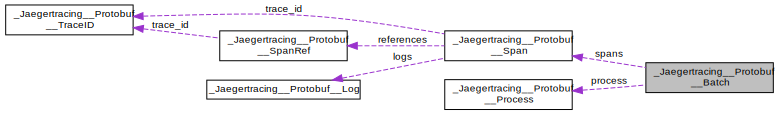
\includegraphics[width=350pt]{struct__Jaegertracing____Protobuf____Batch__coll__graph}
\end{center}
\end{figure}
\subsection*{Data Fields}
\begin{DoxyCompactItemize}
\item 
\mbox{\Hypertarget{struct__Jaegertracing____Protobuf____Batch_aa43b048896fce2d2cca215be2c106640}\label{struct__Jaegertracing____Protobuf____Batch_aa43b048896fce2d2cca215be2c106640}} 
Protobuf\+C\+Message {\bfseries base}
\item 
\mbox{\Hypertarget{struct__Jaegertracing____Protobuf____Batch_a70330d10df460a560fb7c883e01f300c}\label{struct__Jaegertracing____Protobuf____Batch_a70330d10df460a560fb7c883e01f300c}} 
\mbox{\hyperlink{struct__Jaegertracing____Protobuf____Process}{Jaegertracing\+\_\+\+\_\+\+Protobuf\+\_\+\+\_\+\+Process}} $\ast$ {\bfseries process}
\item 
\mbox{\Hypertarget{struct__Jaegertracing____Protobuf____Batch_ad3006039463dc123e716adb10dc3e900}\label{struct__Jaegertracing____Protobuf____Batch_ad3006039463dc123e716adb10dc3e900}} 
size\+\_\+t {\bfseries n\+\_\+spans}
\item 
\mbox{\Hypertarget{struct__Jaegertracing____Protobuf____Batch_a9266661ae189a3ece29e5e7c060efcbd}\label{struct__Jaegertracing____Protobuf____Batch_a9266661ae189a3ece29e5e7c060efcbd}} 
\mbox{\hyperlink{struct__Jaegertracing____Protobuf____Span}{Jaegertracing\+\_\+\+\_\+\+Protobuf\+\_\+\+\_\+\+Span}} $\ast$$\ast$ {\bfseries spans}
\end{DoxyCompactItemize}


The documentation for this struct was generated from the following file\+:\begin{DoxyCompactItemize}
\item 
jaegertracingc/protoc-\/gen/jaeger.\+pb-\/c.\+h\end{DoxyCompactItemize}

\hypertarget{struct__Jaegertracing____Protobuf____BatchResponse}{}\section{\+\_\+\+Jaegertracing\+\_\+\+\_\+\+Protobuf\+\_\+\+\_\+\+Batch\+Response Struct Reference}
\label{struct__Jaegertracing____Protobuf____BatchResponse}\index{\+\_\+\+Jaegertracing\+\_\+\+\_\+\+Protobuf\+\_\+\+\_\+\+Batch\+Response@{\+\_\+\+Jaegertracing\+\_\+\+\_\+\+Protobuf\+\_\+\+\_\+\+Batch\+Response}}
\subsection*{Data Fields}
\begin{DoxyCompactItemize}
\item 
\mbox{\Hypertarget{struct__Jaegertracing____Protobuf____BatchResponse_a60d471d72f383d2fc7bea3d6f548daab}\label{struct__Jaegertracing____Protobuf____BatchResponse_a60d471d72f383d2fc7bea3d6f548daab}} 
Protobuf\+C\+Message {\bfseries base}
\item 
\mbox{\Hypertarget{struct__Jaegertracing____Protobuf____BatchResponse_a8da19ccf0e7189a1197acee1dbd37f8f}\label{struct__Jaegertracing____Protobuf____BatchResponse_a8da19ccf0e7189a1197acee1dbd37f8f}} 
protobuf\+\_\+c\+\_\+boolean {\bfseries ok}
\end{DoxyCompactItemize}


The documentation for this struct was generated from the following file\+:\begin{DoxyCompactItemize}
\item 
jaegertracingc/protoc-\/gen/jaeger.\+pb-\/c.\+h\end{DoxyCompactItemize}

\hypertarget{struct__Jaegertracing____Protobuf____Collector__Service}{}\section{\+\_\+\+Jaegertracing\+\_\+\+\_\+\+Protobuf\+\_\+\+\_\+\+Collector\+\_\+\+Service Struct Reference}
\label{struct__Jaegertracing____Protobuf____Collector__Service}\index{\+\_\+\+Jaegertracing\+\_\+\+\_\+\+Protobuf\+\_\+\+\_\+\+Collector\+\_\+\+Service@{\+\_\+\+Jaegertracing\+\_\+\+\_\+\+Protobuf\+\_\+\+\_\+\+Collector\+\_\+\+Service}}
\subsection*{Data Fields}
\begin{DoxyCompactItemize}
\item 
\mbox{\Hypertarget{struct__Jaegertracing____Protobuf____Collector__Service_abeaffec24ae70f2030955ced727f3431}\label{struct__Jaegertracing____Protobuf____Collector__Service_abeaffec24ae70f2030955ced727f3431}} 
Protobuf\+C\+Service {\bfseries base}
\item 
\mbox{\Hypertarget{struct__Jaegertracing____Protobuf____Collector__Service_ac4502bf1cdb0155aa7f582b3675e6a24}\label{struct__Jaegertracing____Protobuf____Collector__Service_ac4502bf1cdb0155aa7f582b3675e6a24}} 
void($\ast$ {\bfseries submit\+\_\+batches} )(\mbox{\hyperlink{struct__Jaegertracing____Protobuf____Collector__Service}{Jaegertracing\+\_\+\+\_\+\+Protobuf\+\_\+\+\_\+\+Collector\+\_\+\+Service}} $\ast$service, const \mbox{\hyperlink{struct__Jaegertracing____Protobuf____Batch}{Jaegertracing\+\_\+\+\_\+\+Protobuf\+\_\+\+\_\+\+Batch}} $\ast$input, Jaegertracing\+\_\+\+\_\+\+Protobuf\+\_\+\+\_\+\+Batch\+Response\+\_\+\+Closure closure, void $\ast$closure\+\_\+data)
\end{DoxyCompactItemize}


The documentation for this struct was generated from the following file\+:\begin{DoxyCompactItemize}
\item 
jaegertracingc/protoc-\/gen/jaeger.\+pb-\/c.\+h\end{DoxyCompactItemize}

\hypertarget{struct__Jaegertracing____Protobuf____Log}{}\section{\+\_\+\+Jaegertracing\+\_\+\+\_\+\+Protobuf\+\_\+\+\_\+\+Log Struct Reference}
\label{struct__Jaegertracing____Protobuf____Log}\index{\+\_\+\+Jaegertracing\+\_\+\+\_\+\+Protobuf\+\_\+\+\_\+\+Log@{\+\_\+\+Jaegertracing\+\_\+\+\_\+\+Protobuf\+\_\+\+\_\+\+Log}}
\subsection*{Data Fields}
\begin{DoxyCompactItemize}
\item 
\mbox{\Hypertarget{struct__Jaegertracing____Protobuf____Log_a61d97614d14c7f7a6b770e2bacc3d7b4}\label{struct__Jaegertracing____Protobuf____Log_a61d97614d14c7f7a6b770e2bacc3d7b4}} 
Protobuf\+C\+Message {\bfseries base}
\item 
\mbox{\Hypertarget{struct__Jaegertracing____Protobuf____Log_a5c454c324e918baedc5c99d07aff66d1}\label{struct__Jaegertracing____Protobuf____Log_a5c454c324e918baedc5c99d07aff66d1}} 
int64\+\_\+t {\bfseries timestamp}
\item 
\mbox{\Hypertarget{struct__Jaegertracing____Protobuf____Log_ad9ba7daed1f1e1d273f22b4a03499aa4}\label{struct__Jaegertracing____Protobuf____Log_ad9ba7daed1f1e1d273f22b4a03499aa4}} 
size\+\_\+t {\bfseries n\+\_\+fields}
\item 
\mbox{\Hypertarget{struct__Jaegertracing____Protobuf____Log_af6a10f540b191616231931279af25add}\label{struct__Jaegertracing____Protobuf____Log_af6a10f540b191616231931279af25add}} 
Jaegertracing\+\_\+\+\_\+\+Protobuf\+\_\+\+\_\+\+Tag $\ast$$\ast$ {\bfseries fields}
\end{DoxyCompactItemize}


The documentation for this struct was generated from the following file\+:\begin{DoxyCompactItemize}
\item 
jaegertracingc/protoc-\/gen/jaeger.\+pb-\/c.\+h\end{DoxyCompactItemize}

\hypertarget{struct__Jaegertracing____Protobuf____Process}{}\section{\+\_\+\+Jaegertracing\+\_\+\+\_\+\+Protobuf\+\_\+\+\_\+\+Process Struct Reference}
\label{struct__Jaegertracing____Protobuf____Process}\index{\+\_\+\+Jaegertracing\+\_\+\+\_\+\+Protobuf\+\_\+\+\_\+\+Process@{\+\_\+\+Jaegertracing\+\_\+\+\_\+\+Protobuf\+\_\+\+\_\+\+Process}}
\subsection*{Data Fields}
\begin{DoxyCompactItemize}
\item 
\mbox{\Hypertarget{struct__Jaegertracing____Protobuf____Process_ae8195593faa6c882368973fe424804ec}\label{struct__Jaegertracing____Protobuf____Process_ae8195593faa6c882368973fe424804ec}} 
Protobuf\+C\+Message {\bfseries base}
\item 
\mbox{\Hypertarget{struct__Jaegertracing____Protobuf____Process_a76cc3d4c5e0de7a533b201a4bc23bc09}\label{struct__Jaegertracing____Protobuf____Process_a76cc3d4c5e0de7a533b201a4bc23bc09}} 
char $\ast$ {\bfseries service\+\_\+name}
\item 
\mbox{\Hypertarget{struct__Jaegertracing____Protobuf____Process_a3c1cefa717abb1be371a45d87e2dd91d}\label{struct__Jaegertracing____Protobuf____Process_a3c1cefa717abb1be371a45d87e2dd91d}} 
size\+\_\+t {\bfseries n\+\_\+tags}
\item 
\mbox{\Hypertarget{struct__Jaegertracing____Protobuf____Process_a4ee1a205145e6abe6b0b36381c0ef650}\label{struct__Jaegertracing____Protobuf____Process_a4ee1a205145e6abe6b0b36381c0ef650}} 
Jaegertracing\+\_\+\+\_\+\+Protobuf\+\_\+\+\_\+\+Tag $\ast$$\ast$ {\bfseries tags}
\end{DoxyCompactItemize}


The documentation for this struct was generated from the following file\+:\begin{DoxyCompactItemize}
\item 
jaegertracingc/protoc-\/gen/jaeger.\+pb-\/c.\+h\end{DoxyCompactItemize}

\hypertarget{struct__Jaegertracing____Protobuf____SamplingManager____PerOperationSamplingStrategy}{}\section{\+\_\+\+Jaegertracing\+\_\+\+\_\+\+Protobuf\+\_\+\+\_\+\+Sampling\+Manager\+\_\+\+\_\+\+Per\+Operation\+Sampling\+Strategy Struct Reference}
\label{struct__Jaegertracing____Protobuf____SamplingManager____PerOperationSamplingStrategy}\index{\+\_\+\+Jaegertracing\+\_\+\+\_\+\+Protobuf\+\_\+\+\_\+\+Sampling\+Manager\+\_\+\+\_\+\+Per\+Operation\+Sampling\+Strategy@{\+\_\+\+Jaegertracing\+\_\+\+\_\+\+Protobuf\+\_\+\+\_\+\+Sampling\+Manager\+\_\+\+\_\+\+Per\+Operation\+Sampling\+Strategy}}


Collaboration diagram for \+\_\+\+Jaegertracing\+\_\+\+\_\+\+Protobuf\+\_\+\+\_\+\+Sampling\+Manager\+\_\+\+\_\+\+Per\+Operation\+Sampling\+Strategy\+:
\nopagebreak
\begin{figure}[H]
\begin{center}
\leavevmode
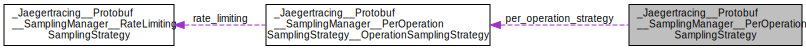
\includegraphics[width=350pt]{struct__Jaegertracing____Protobuf____SamplingManager____PerOperationSamplingStrategy__coll__graph}
\end{center}
\end{figure}
\subsection*{Data Fields}
\begin{DoxyCompactItemize}
\item 
\mbox{\Hypertarget{struct__Jaegertracing____Protobuf____SamplingManager____PerOperationSamplingStrategy_a68a1b18890023153e365d9fb9eecfac7}\label{struct__Jaegertracing____Protobuf____SamplingManager____PerOperationSamplingStrategy_a68a1b18890023153e365d9fb9eecfac7}} 
Protobuf\+C\+Message {\bfseries base}
\item 
\mbox{\Hypertarget{struct__Jaegertracing____Protobuf____SamplingManager____PerOperationSamplingStrategy_a99f02545f9bf9397a1d45da4d810f265}\label{struct__Jaegertracing____Protobuf____SamplingManager____PerOperationSamplingStrategy_a99f02545f9bf9397a1d45da4d810f265}} 
double {\bfseries default\+\_\+sampling\+\_\+probability}
\item 
\mbox{\Hypertarget{struct__Jaegertracing____Protobuf____SamplingManager____PerOperationSamplingStrategy_a0f03dcadd349c4b1005b55837c518580}\label{struct__Jaegertracing____Protobuf____SamplingManager____PerOperationSamplingStrategy_a0f03dcadd349c4b1005b55837c518580}} 
double {\bfseries default\+\_\+lower\+\_\+bound\+\_\+traces\+\_\+per\+\_\+second}
\item 
\mbox{\Hypertarget{struct__Jaegertracing____Protobuf____SamplingManager____PerOperationSamplingStrategy_a8aa2f4f89992ebafb082ee6b6fd8ecff}\label{struct__Jaegertracing____Protobuf____SamplingManager____PerOperationSamplingStrategy_a8aa2f4f89992ebafb082ee6b6fd8ecff}} 
double {\bfseries default\+\_\+upper\+\_\+bound\+\_\+traces\+\_\+per\+\_\+second}
\item 
\mbox{\Hypertarget{struct__Jaegertracing____Protobuf____SamplingManager____PerOperationSamplingStrategy_a636b2d5dad99a8dc1e67a310c240023a}\label{struct__Jaegertracing____Protobuf____SamplingManager____PerOperationSamplingStrategy_a636b2d5dad99a8dc1e67a310c240023a}} 
size\+\_\+t {\bfseries n\+\_\+per\+\_\+operation\+\_\+strategy}
\item 
\mbox{\Hypertarget{struct__Jaegertracing____Protobuf____SamplingManager____PerOperationSamplingStrategy_a64bd6d5d797c89d3f700d8c4a6914901}\label{struct__Jaegertracing____Protobuf____SamplingManager____PerOperationSamplingStrategy_a64bd6d5d797c89d3f700d8c4a6914901}} 
\mbox{\hyperlink{struct__Jaegertracing____Protobuf____SamplingManager____PerOperationSamplingStrategy____OperationSamplingStrategy}{Jaegertracing\+\_\+\+\_\+\+Protobuf\+\_\+\+\_\+\+Sampling\+Manager\+\_\+\+\_\+\+Per\+Operation\+Sampling\+Strategy\+\_\+\+\_\+\+Operation\+Sampling\+Strategy}} $\ast$$\ast$ {\bfseries per\+\_\+operation\+\_\+strategy}
\end{DoxyCompactItemize}


The documentation for this struct was generated from the following file\+:\begin{DoxyCompactItemize}
\item 
jaegertracingc/protoc-\/gen/sampling.\+pb-\/c.\+h\end{DoxyCompactItemize}

\hypertarget{struct__Jaegertracing____Protobuf____SamplingManager____PerOperationSamplingStrategy____OperationSamplingStrategy}{}\section{\+\_\+\+Jaegertracing\+\_\+\+\_\+\+Protobuf\+\_\+\+\_\+\+Sampling\+Manager\+\_\+\+\_\+\+Per\+Operation\+Sampling\+Strategy\+\_\+\+\_\+\+Operation\+Sampling\+Strategy Struct Reference}
\label{struct__Jaegertracing____Protobuf____SamplingManager____PerOperationSamplingStrategy____OperationSamplingStrategy}\index{\+\_\+\+Jaegertracing\+\_\+\+\_\+\+Protobuf\+\_\+\+\_\+\+Sampling\+Manager\+\_\+\+\_\+\+Per\+Operation\+Sampling\+Strategy\+\_\+\+\_\+\+Operation\+Sampling\+Strategy@{\+\_\+\+Jaegertracing\+\_\+\+\_\+\+Protobuf\+\_\+\+\_\+\+Sampling\+Manager\+\_\+\+\_\+\+Per\+Operation\+Sampling\+Strategy\+\_\+\+\_\+\+Operation\+Sampling\+Strategy}}


Collaboration diagram for \+\_\+\+Jaegertracing\+\_\+\+\_\+\+Protobuf\+\_\+\+\_\+\+Sampling\+Manager\+\_\+\+\_\+\+Per\+Operation\+Sampling\+Strategy\+\_\+\+\_\+\+Operation\+Sampling\+Strategy\+:
\nopagebreak
\begin{figure}[H]
\begin{center}
\leavevmode
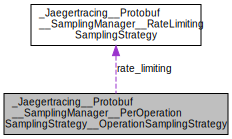
\includegraphics[width=304pt]{struct__Jaegertracing____Protobuf____SamplingManager____PerOperationSamplingStrategy____OperationSamplingStrategy__coll__graph}
\end{center}
\end{figure}
\subsection*{Data Fields}
\begin{DoxyCompactItemize}
\item 
\mbox{\Hypertarget{struct__Jaegertracing____Protobuf____SamplingManager____PerOperationSamplingStrategy____OperationSamplingStrategy_add0d0327453eac9421bc4f96a271d18a}\label{struct__Jaegertracing____Protobuf____SamplingManager____PerOperationSamplingStrategy____OperationSamplingStrategy_add0d0327453eac9421bc4f96a271d18a}} 
Protobuf\+C\+Message {\bfseries base}
\item 
\mbox{\Hypertarget{struct__Jaegertracing____Protobuf____SamplingManager____PerOperationSamplingStrategy____OperationSamplingStrategy_ae3e65181bbe7873e7d7bd30083b4eb51}\label{struct__Jaegertracing____Protobuf____SamplingManager____PerOperationSamplingStrategy____OperationSamplingStrategy_ae3e65181bbe7873e7d7bd30083b4eb51}} 
char $\ast$ {\bfseries operation}
\item 
\mbox{\Hypertarget{struct__Jaegertracing____Protobuf____SamplingManager____PerOperationSamplingStrategy____OperationSamplingStrategy_a3b268b07f41b0fbc60ebff3c8ad36d37}\label{struct__Jaegertracing____Protobuf____SamplingManager____PerOperationSamplingStrategy____OperationSamplingStrategy_a3b268b07f41b0fbc60ebff3c8ad36d37}} 
Jaegertracing\+\_\+\+\_\+\+Protobuf\+\_\+\+\_\+\+Sampling\+Manager\+\_\+\+\_\+\+Per\+Operation\+Sampling\+Strategy\+\_\+\+\_\+\+Operation\+Sampling\+Strategy\+\_\+\+\_\+\+Strategy\+Case {\bfseries strategy\+\_\+case}
\item 
\mbox{\Hypertarget{struct__Jaegertracing____Protobuf____SamplingManager____PerOperationSamplingStrategy____OperationSamplingStrategy_a069bcc0b742650991206f155e5b0f972}\label{struct__Jaegertracing____Protobuf____SamplingManager____PerOperationSamplingStrategy____OperationSamplingStrategy_a069bcc0b742650991206f155e5b0f972}} 
\begin{tabbing}
xx\=xx\=xx\=xx\=xx\=xx\=xx\=xx\=xx\=\kill
union \{\\
\>Jaegertracing\_\_Protobuf\_\_SamplingManager\_\_ProbabilisticSamplingStrategy $\ast$ {\bfseries probabilistic}\\
\>\mbox{\hyperlink{struct__Jaegertracing____Protobuf____SamplingManager____RateLimitingSamplingStrategy}{Jaegertracing\_\_Protobuf\_\_SamplingManager\_\_RateLimitingSamplingStrategy}} $\ast$ {\bfseries rate\_limiting}\\
\}; \\

\end{tabbing}\end{DoxyCompactItemize}


The documentation for this struct was generated from the following file\+:\begin{DoxyCompactItemize}
\item 
jaegertracingc/protoc-\/gen/sampling.\+pb-\/c.\+h\end{DoxyCompactItemize}

\hypertarget{struct__Jaegertracing____Protobuf____SamplingManager____ProbabilisticSamplingStrategy}{}\section{\+\_\+\+Jaegertracing\+\_\+\+\_\+\+Protobuf\+\_\+\+\_\+\+Sampling\+Manager\+\_\+\+\_\+\+Probabilistic\+Sampling\+Strategy Struct Reference}
\label{struct__Jaegertracing____Protobuf____SamplingManager____ProbabilisticSamplingStrategy}\index{\+\_\+\+Jaegertracing\+\_\+\+\_\+\+Protobuf\+\_\+\+\_\+\+Sampling\+Manager\+\_\+\+\_\+\+Probabilistic\+Sampling\+Strategy@{\+\_\+\+Jaegertracing\+\_\+\+\_\+\+Protobuf\+\_\+\+\_\+\+Sampling\+Manager\+\_\+\+\_\+\+Probabilistic\+Sampling\+Strategy}}
\subsection*{Data Fields}
\begin{DoxyCompactItemize}
\item 
\mbox{\Hypertarget{struct__Jaegertracing____Protobuf____SamplingManager____ProbabilisticSamplingStrategy_a4354f095f0e49c79abfbc7f786be6b41}\label{struct__Jaegertracing____Protobuf____SamplingManager____ProbabilisticSamplingStrategy_a4354f095f0e49c79abfbc7f786be6b41}} 
Protobuf\+C\+Message {\bfseries base}
\item 
\mbox{\Hypertarget{struct__Jaegertracing____Protobuf____SamplingManager____ProbabilisticSamplingStrategy_a191605c4af2a8294cefe0c50573fc4c7}\label{struct__Jaegertracing____Protobuf____SamplingManager____ProbabilisticSamplingStrategy_a191605c4af2a8294cefe0c50573fc4c7}} 
double {\bfseries sampling\+\_\+rate}
\end{DoxyCompactItemize}


The documentation for this struct was generated from the following file\+:\begin{DoxyCompactItemize}
\item 
jaegertracingc/protoc-\/gen/sampling.\+pb-\/c.\+h\end{DoxyCompactItemize}

\hypertarget{struct__Jaegertracing____Protobuf____SamplingManager____RateLimitingSamplingStrategy}{}\section{\+\_\+\+Jaegertracing\+\_\+\+\_\+\+Protobuf\+\_\+\+\_\+\+Sampling\+Manager\+\_\+\+\_\+\+Rate\+Limiting\+Sampling\+Strategy Struct Reference}
\label{struct__Jaegertracing____Protobuf____SamplingManager____RateLimitingSamplingStrategy}\index{\+\_\+\+Jaegertracing\+\_\+\+\_\+\+Protobuf\+\_\+\+\_\+\+Sampling\+Manager\+\_\+\+\_\+\+Rate\+Limiting\+Sampling\+Strategy@{\+\_\+\+Jaegertracing\+\_\+\+\_\+\+Protobuf\+\_\+\+\_\+\+Sampling\+Manager\+\_\+\+\_\+\+Rate\+Limiting\+Sampling\+Strategy}}
\subsection*{Data Fields}
\begin{DoxyCompactItemize}
\item 
\mbox{\Hypertarget{struct__Jaegertracing____Protobuf____SamplingManager____RateLimitingSamplingStrategy_a796a0f18fc2f503c0b6986c547283eaa}\label{struct__Jaegertracing____Protobuf____SamplingManager____RateLimitingSamplingStrategy_a796a0f18fc2f503c0b6986c547283eaa}} 
Protobuf\+C\+Message {\bfseries base}
\item 
\mbox{\Hypertarget{struct__Jaegertracing____Protobuf____SamplingManager____RateLimitingSamplingStrategy_a2fe496a01a9eff8b38c97d67565cd182}\label{struct__Jaegertracing____Protobuf____SamplingManager____RateLimitingSamplingStrategy_a2fe496a01a9eff8b38c97d67565cd182}} 
int32\+\_\+t {\bfseries max\+\_\+traces\+\_\+per\+\_\+second}
\end{DoxyCompactItemize}


The documentation for this struct was generated from the following file\+:\begin{DoxyCompactItemize}
\item 
jaegertracingc/protoc-\/gen/sampling.\+pb-\/c.\+h\end{DoxyCompactItemize}

\hypertarget{struct__Jaegertracing____Protobuf____SamplingManager____SamplingManager__Service}{}\section{\+\_\+\+Jaegertracing\+\_\+\+\_\+\+Protobuf\+\_\+\+\_\+\+Sampling\+Manager\+\_\+\+\_\+\+Sampling\+Manager\+\_\+\+Service Struct Reference}
\label{struct__Jaegertracing____Protobuf____SamplingManager____SamplingManager__Service}\index{\+\_\+\+Jaegertracing\+\_\+\+\_\+\+Protobuf\+\_\+\+\_\+\+Sampling\+Manager\+\_\+\+\_\+\+Sampling\+Manager\+\_\+\+Service@{\+\_\+\+Jaegertracing\+\_\+\+\_\+\+Protobuf\+\_\+\+\_\+\+Sampling\+Manager\+\_\+\+\_\+\+Sampling\+Manager\+\_\+\+Service}}
\subsection*{Data Fields}
\begin{DoxyCompactItemize}
\item 
\mbox{\Hypertarget{struct__Jaegertracing____Protobuf____SamplingManager____SamplingManager__Service_a148ac6a9a054775bb1c7a3c97eb0b80c}\label{struct__Jaegertracing____Protobuf____SamplingManager____SamplingManager__Service_a148ac6a9a054775bb1c7a3c97eb0b80c}} 
Protobuf\+C\+Service {\bfseries base}
\item 
\mbox{\Hypertarget{struct__Jaegertracing____Protobuf____SamplingManager____SamplingManager__Service_aa88c98562fdf0a68b2ccecb8f5b795b0}\label{struct__Jaegertracing____Protobuf____SamplingManager____SamplingManager__Service_aa88c98562fdf0a68b2ccecb8f5b795b0}} 
void($\ast$ {\bfseries get\+\_\+sampling\+\_\+strategy} )(\mbox{\hyperlink{struct__Jaegertracing____Protobuf____SamplingManager____SamplingManager__Service}{Jaegertracing\+\_\+\+\_\+\+Protobuf\+\_\+\+\_\+\+Sampling\+Manager\+\_\+\+\_\+\+Sampling\+Manager\+\_\+\+Service}} $\ast$service, const \mbox{\hyperlink{struct__Jaegertracing____Protobuf____SamplingManager____SamplingStrategyRequest}{Jaegertracing\+\_\+\+\_\+\+Protobuf\+\_\+\+\_\+\+Sampling\+Manager\+\_\+\+\_\+\+Sampling\+Strategy\+Request}} $\ast$input, Jaegertracing\+\_\+\+\_\+\+Protobuf\+\_\+\+\_\+\+Sampling\+Manager\+\_\+\+\_\+\+Sampling\+Strategy\+Response\+\_\+\+Closure closure, void $\ast$closure\+\_\+data)
\end{DoxyCompactItemize}


The documentation for this struct was generated from the following file\+:\begin{DoxyCompactItemize}
\item 
jaegertracingc/protoc-\/gen/sampling.\+pb-\/c.\+h\end{DoxyCompactItemize}

\hypertarget{struct__Jaegertracing____Protobuf____SamplingManager____SamplingStrategyRequest}{}\section{\+\_\+\+Jaegertracing\+\_\+\+\_\+\+Protobuf\+\_\+\+\_\+\+Sampling\+Manager\+\_\+\+\_\+\+Sampling\+Strategy\+Request Struct Reference}
\label{struct__Jaegertracing____Protobuf____SamplingManager____SamplingStrategyRequest}\index{\+\_\+\+Jaegertracing\+\_\+\+\_\+\+Protobuf\+\_\+\+\_\+\+Sampling\+Manager\+\_\+\+\_\+\+Sampling\+Strategy\+Request@{\+\_\+\+Jaegertracing\+\_\+\+\_\+\+Protobuf\+\_\+\+\_\+\+Sampling\+Manager\+\_\+\+\_\+\+Sampling\+Strategy\+Request}}
\subsection*{Data Fields}
\begin{DoxyCompactItemize}
\item 
\mbox{\Hypertarget{struct__Jaegertracing____Protobuf____SamplingManager____SamplingStrategyRequest_ae56c67a98c43e9b6e03a58e6cdd88467}\label{struct__Jaegertracing____Protobuf____SamplingManager____SamplingStrategyRequest_ae56c67a98c43e9b6e03a58e6cdd88467}} 
Protobuf\+C\+Message {\bfseries base}
\item 
\mbox{\Hypertarget{struct__Jaegertracing____Protobuf____SamplingManager____SamplingStrategyRequest_a854b0e0744b64ce1197ba7dbe5e7c48c}\label{struct__Jaegertracing____Protobuf____SamplingManager____SamplingStrategyRequest_a854b0e0744b64ce1197ba7dbe5e7c48c}} 
char $\ast$ {\bfseries service\+\_\+name}
\end{DoxyCompactItemize}


The documentation for this struct was generated from the following file\+:\begin{DoxyCompactItemize}
\item 
jaegertracingc/protoc-\/gen/sampling.\+pb-\/c.\+h\end{DoxyCompactItemize}

\hypertarget{struct__Jaegertracing____Protobuf____SamplingManager____SamplingStrategyResponse}{}\section{\+\_\+\+Jaegertracing\+\_\+\+\_\+\+Protobuf\+\_\+\+\_\+\+Sampling\+Manager\+\_\+\+\_\+\+Sampling\+Strategy\+Response Struct Reference}
\label{struct__Jaegertracing____Protobuf____SamplingManager____SamplingStrategyResponse}\index{\+\_\+\+Jaegertracing\+\_\+\+\_\+\+Protobuf\+\_\+\+\_\+\+Sampling\+Manager\+\_\+\+\_\+\+Sampling\+Strategy\+Response@{\+\_\+\+Jaegertracing\+\_\+\+\_\+\+Protobuf\+\_\+\+\_\+\+Sampling\+Manager\+\_\+\+\_\+\+Sampling\+Strategy\+Response}}


Collaboration diagram for \+\_\+\+Jaegertracing\+\_\+\+\_\+\+Protobuf\+\_\+\+\_\+\+Sampling\+Manager\+\_\+\+\_\+\+Sampling\+Strategy\+Response\+:
\nopagebreak
\begin{figure}[H]
\begin{center}
\leavevmode
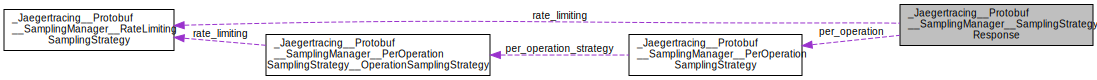
\includegraphics[width=350pt]{struct__Jaegertracing____Protobuf____SamplingManager____SamplingStrategyResponse__coll__graph}
\end{center}
\end{figure}
\subsection*{Data Fields}
\begin{DoxyCompactItemize}
\item 
\mbox{\Hypertarget{struct__Jaegertracing____Protobuf____SamplingManager____SamplingStrategyResponse_a888d5c3298752e9d8918475944738692}\label{struct__Jaegertracing____Protobuf____SamplingManager____SamplingStrategyResponse_a888d5c3298752e9d8918475944738692}} 
Protobuf\+C\+Message {\bfseries base}
\item 
\mbox{\Hypertarget{struct__Jaegertracing____Protobuf____SamplingManager____SamplingStrategyResponse_ad0e1de7ecc2ef6ccbe9936c701380150}\label{struct__Jaegertracing____Protobuf____SamplingManager____SamplingStrategyResponse_ad0e1de7ecc2ef6ccbe9936c701380150}} 
Jaegertracing\+\_\+\+\_\+\+Protobuf\+\_\+\+\_\+\+Sampling\+Manager\+\_\+\+\_\+\+Sampling\+Strategy\+Response\+\_\+\+\_\+\+Strategy\+Case {\bfseries strategy\+\_\+case}
\item 
\mbox{\Hypertarget{struct__Jaegertracing____Protobuf____SamplingManager____SamplingStrategyResponse_af3398ad3890a72d6708ed91f1e61dd5b}\label{struct__Jaegertracing____Protobuf____SamplingManager____SamplingStrategyResponse_af3398ad3890a72d6708ed91f1e61dd5b}} 
\begin{tabbing}
xx\=xx\=xx\=xx\=xx\=xx\=xx\=xx\=xx\=\kill
union \{\\
\>Jaegertracing\_\_Protobuf\_\_SamplingManager\_\_ProbabilisticSamplingStrategy $\ast$ {\bfseries probabilistic}\\
\>\mbox{\hyperlink{struct__Jaegertracing____Protobuf____SamplingManager____RateLimitingSamplingStrategy}{Jaegertracing\_\_Protobuf\_\_SamplingManager\_\_RateLimitingSamplingStrategy}} $\ast$ {\bfseries rate\_limiting}\\
\>\mbox{\hyperlink{struct__Jaegertracing____Protobuf____SamplingManager____PerOperationSamplingStrategy}{Jaegertracing\_\_Protobuf\_\_SamplingManager\_\_PerOperationSamplingStrategy}} $\ast$ {\bfseries per\_operation}\\
\}; \\

\end{tabbing}\end{DoxyCompactItemize}


The documentation for this struct was generated from the following file\+:\begin{DoxyCompactItemize}
\item 
jaegertracingc/protoc-\/gen/sampling.\+pb-\/c.\+h\end{DoxyCompactItemize}

\hypertarget{struct__Jaegertracing____Protobuf____Span}{}\section{\+\_\+\+Jaegertracing\+\_\+\+\_\+\+Protobuf\+\_\+\+\_\+\+Span Struct Reference}
\label{struct__Jaegertracing____Protobuf____Span}\index{\+\_\+\+Jaegertracing\+\_\+\+\_\+\+Protobuf\+\_\+\+\_\+\+Span@{\+\_\+\+Jaegertracing\+\_\+\+\_\+\+Protobuf\+\_\+\+\_\+\+Span}}


Collaboration diagram for \+\_\+\+Jaegertracing\+\_\+\+\_\+\+Protobuf\+\_\+\+\_\+\+Span\+:
\nopagebreak
\begin{figure}[H]
\begin{center}
\leavevmode
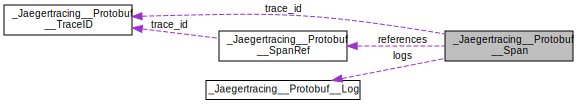
\includegraphics[width=350pt]{struct__Jaegertracing____Protobuf____Span__coll__graph}
\end{center}
\end{figure}
\subsection*{Data Fields}
\begin{DoxyCompactItemize}
\item 
\mbox{\Hypertarget{struct__Jaegertracing____Protobuf____Span_aa6c240264dd438078c15ac687f580c9a}\label{struct__Jaegertracing____Protobuf____Span_aa6c240264dd438078c15ac687f580c9a}} 
Protobuf\+C\+Message {\bfseries base}
\item 
\mbox{\Hypertarget{struct__Jaegertracing____Protobuf____Span_aeadc1704486abe90cb503440ff9ba891}\label{struct__Jaegertracing____Protobuf____Span_aeadc1704486abe90cb503440ff9ba891}} 
\mbox{\hyperlink{struct__Jaegertracing____Protobuf____TraceID}{Jaegertracing\+\_\+\+\_\+\+Protobuf\+\_\+\+\_\+\+Trace\+ID}} $\ast$ {\bfseries trace\+\_\+id}
\item 
\mbox{\Hypertarget{struct__Jaegertracing____Protobuf____Span_ac84e0ef1c107b63aa87183c6f7f10fa3}\label{struct__Jaegertracing____Protobuf____Span_ac84e0ef1c107b63aa87183c6f7f10fa3}} 
uint64\+\_\+t {\bfseries span\+\_\+id}
\item 
\mbox{\Hypertarget{struct__Jaegertracing____Protobuf____Span_aaa3a5c136dfa47f819c85c427741bd71}\label{struct__Jaegertracing____Protobuf____Span_aaa3a5c136dfa47f819c85c427741bd71}} 
uint64\+\_\+t {\bfseries parent\+\_\+span\+\_\+id}
\item 
\mbox{\Hypertarget{struct__Jaegertracing____Protobuf____Span_a8db3ea41e551c65cb74e2d5d38f3f8e3}\label{struct__Jaegertracing____Protobuf____Span_a8db3ea41e551c65cb74e2d5d38f3f8e3}} 
char $\ast$ {\bfseries operation\+\_\+name}
\item 
\mbox{\Hypertarget{struct__Jaegertracing____Protobuf____Span_af139c7207e186524a8eaeaf13e53cd07}\label{struct__Jaegertracing____Protobuf____Span_af139c7207e186524a8eaeaf13e53cd07}} 
size\+\_\+t {\bfseries n\+\_\+references}
\item 
\mbox{\Hypertarget{struct__Jaegertracing____Protobuf____Span_a6702db49dcd1153df681ed4489a1c6ad}\label{struct__Jaegertracing____Protobuf____Span_a6702db49dcd1153df681ed4489a1c6ad}} 
\mbox{\hyperlink{struct__Jaegertracing____Protobuf____SpanRef}{Jaegertracing\+\_\+\+\_\+\+Protobuf\+\_\+\+\_\+\+Span\+Ref}} $\ast$$\ast$ {\bfseries references}
\item 
\mbox{\Hypertarget{struct__Jaegertracing____Protobuf____Span_a4908eb7263b6cda22d19bbc4e49d1cdb}\label{struct__Jaegertracing____Protobuf____Span_a4908eb7263b6cda22d19bbc4e49d1cdb}} 
int32\+\_\+t {\bfseries flags}
\item 
\mbox{\Hypertarget{struct__Jaegertracing____Protobuf____Span_a4a54ffe66c26e6584cfa8bcafe723b63}\label{struct__Jaegertracing____Protobuf____Span_a4a54ffe66c26e6584cfa8bcafe723b63}} 
int64\+\_\+t {\bfseries start\+\_\+time}
\item 
\mbox{\Hypertarget{struct__Jaegertracing____Protobuf____Span_ad7326e11a1584dabc69d7fbf2b9d0931}\label{struct__Jaegertracing____Protobuf____Span_ad7326e11a1584dabc69d7fbf2b9d0931}} 
int64\+\_\+t {\bfseries duration}
\item 
\mbox{\Hypertarget{struct__Jaegertracing____Protobuf____Span_a58c542c87e75e5f05b7bf297ed8851bf}\label{struct__Jaegertracing____Protobuf____Span_a58c542c87e75e5f05b7bf297ed8851bf}} 
size\+\_\+t {\bfseries n\+\_\+tags}
\item 
\mbox{\Hypertarget{struct__Jaegertracing____Protobuf____Span_a35dcc7640937b6f5744e0c61f418680d}\label{struct__Jaegertracing____Protobuf____Span_a35dcc7640937b6f5744e0c61f418680d}} 
Jaegertracing\+\_\+\+\_\+\+Protobuf\+\_\+\+\_\+\+Tag $\ast$$\ast$ {\bfseries tags}
\item 
\mbox{\Hypertarget{struct__Jaegertracing____Protobuf____Span_aa2b5d2e1b9619bd294d1b2360c910f99}\label{struct__Jaegertracing____Protobuf____Span_aa2b5d2e1b9619bd294d1b2360c910f99}} 
size\+\_\+t {\bfseries n\+\_\+logs}
\item 
\mbox{\Hypertarget{struct__Jaegertracing____Protobuf____Span_a7be0e70cb55edf1b95f4489bff73dda3}\label{struct__Jaegertracing____Protobuf____Span_a7be0e70cb55edf1b95f4489bff73dda3}} 
\mbox{\hyperlink{struct__Jaegertracing____Protobuf____Log}{Jaegertracing\+\_\+\+\_\+\+Protobuf\+\_\+\+\_\+\+Log}} $\ast$$\ast$ {\bfseries logs}
\end{DoxyCompactItemize}


The documentation for this struct was generated from the following file\+:\begin{DoxyCompactItemize}
\item 
jaegertracingc/protoc-\/gen/jaeger.\+pb-\/c.\+h\end{DoxyCompactItemize}

\hypertarget{struct__Jaegertracing____Protobuf____SpanRef}{}\section{\+\_\+\+Jaegertracing\+\_\+\+\_\+\+Protobuf\+\_\+\+\_\+\+Span\+Ref Struct Reference}
\label{struct__Jaegertracing____Protobuf____SpanRef}\index{\+\_\+\+Jaegertracing\+\_\+\+\_\+\+Protobuf\+\_\+\+\_\+\+Span\+Ref@{\+\_\+\+Jaegertracing\+\_\+\+\_\+\+Protobuf\+\_\+\+\_\+\+Span\+Ref}}


Collaboration diagram for \+\_\+\+Jaegertracing\+\_\+\+\_\+\+Protobuf\+\_\+\+\_\+\+Span\+Ref\+:
\nopagebreak
\begin{figure}[H]
\begin{center}
\leavevmode
\includegraphics[width=208pt]{struct__Jaegertracing____Protobuf____SpanRef__coll__graph}
\end{center}
\end{figure}
\subsection*{Data Fields}
\begin{DoxyCompactItemize}
\item 
\mbox{\Hypertarget{struct__Jaegertracing____Protobuf____SpanRef_a8034208957bece0b408cea9cd6015b98}\label{struct__Jaegertracing____Protobuf____SpanRef_a8034208957bece0b408cea9cd6015b98}} 
Protobuf\+C\+Message {\bfseries base}
\item 
\mbox{\Hypertarget{struct__Jaegertracing____Protobuf____SpanRef_acf330d0ea738d0fac8cd3038ad1b8261}\label{struct__Jaegertracing____Protobuf____SpanRef_acf330d0ea738d0fac8cd3038ad1b8261}} 
Jaegertracing\+\_\+\+\_\+\+Protobuf\+\_\+\+\_\+\+Span\+Ref\+\_\+\+\_\+\+Type {\bfseries type}
\item 
\mbox{\Hypertarget{struct__Jaegertracing____Protobuf____SpanRef_aaa4464a336d9d2c6c0197264dfa22314}\label{struct__Jaegertracing____Protobuf____SpanRef_aaa4464a336d9d2c6c0197264dfa22314}} 
\mbox{\hyperlink{struct__Jaegertracing____Protobuf____TraceID}{Jaegertracing\+\_\+\+\_\+\+Protobuf\+\_\+\+\_\+\+Trace\+ID}} $\ast$ {\bfseries trace\+\_\+id}
\item 
\mbox{\Hypertarget{struct__Jaegertracing____Protobuf____SpanRef_a639ed6c4e8ce8ebc0f711367bd7603cf}\label{struct__Jaegertracing____Protobuf____SpanRef_a639ed6c4e8ce8ebc0f711367bd7603cf}} 
uint64\+\_\+t {\bfseries span\+\_\+id}
\end{DoxyCompactItemize}


The documentation for this struct was generated from the following file\+:\begin{DoxyCompactItemize}
\item 
jaegertracingc/protoc-\/gen/jaeger.\+pb-\/c.\+h\end{DoxyCompactItemize}

\hypertarget{struct__Jaegertracing____Protobuf____Tag}{}\section{\+\_\+\+Jaegertracing\+\_\+\+\_\+\+Protobuf\+\_\+\+\_\+\+Tag Struct Reference}
\label{struct__Jaegertracing____Protobuf____Tag}\index{\+\_\+\+Jaegertracing\+\_\+\+\_\+\+Protobuf\+\_\+\+\_\+\+Tag@{\+\_\+\+Jaegertracing\+\_\+\+\_\+\+Protobuf\+\_\+\+\_\+\+Tag}}
\subsection*{Data Fields}
\begin{DoxyCompactItemize}
\item 
\mbox{\Hypertarget{struct__Jaegertracing____Protobuf____Tag_a5083777cfc630087e26728b68718c770}\label{struct__Jaegertracing____Protobuf____Tag_a5083777cfc630087e26728b68718c770}} 
Protobuf\+C\+Message {\bfseries base}
\item 
\mbox{\Hypertarget{struct__Jaegertracing____Protobuf____Tag_a3ae221578bff2b92ee29a14bfb7400be}\label{struct__Jaegertracing____Protobuf____Tag_a3ae221578bff2b92ee29a14bfb7400be}} 
char $\ast$ {\bfseries key}
\item 
\mbox{\Hypertarget{struct__Jaegertracing____Protobuf____Tag_a191aadd4272a839677f3e9aa09524623}\label{struct__Jaegertracing____Protobuf____Tag_a191aadd4272a839677f3e9aa09524623}} 
Jaegertracing\+\_\+\+\_\+\+Protobuf\+\_\+\+\_\+\+Tag\+\_\+\+\_\+\+Value\+Case {\bfseries value\+\_\+case}
\item 
\mbox{\Hypertarget{struct__Jaegertracing____Protobuf____Tag_ab776beb7bf63c2e99057d1284a0b8e6a}\label{struct__Jaegertracing____Protobuf____Tag_ab776beb7bf63c2e99057d1284a0b8e6a}} 
\begin{tabbing}
xx\=xx\=xx\=xx\=xx\=xx\=xx\=xx\=xx\=\kill
union \{\\
\>char $\ast$ {\bfseries str\_value}\\
\>double {\bfseries double\_value}\\
\>protobuf\_c\_boolean {\bfseries bool\_value}\\
\>int64\_t {\bfseries long\_value}\\
\>ProtobufCBinaryData {\bfseries binary\_value}\\
\}; \\

\end{tabbing}\end{DoxyCompactItemize}


The documentation for this struct was generated from the following file\+:\begin{DoxyCompactItemize}
\item 
jaegertracingc/protoc-\/gen/jaeger.\+pb-\/c.\+h\end{DoxyCompactItemize}

\hypertarget{struct__Jaegertracing____Protobuf____TraceID}{}\section{\+\_\+\+Jaegertracing\+\_\+\+\_\+\+Protobuf\+\_\+\+\_\+\+Trace\+ID Struct Reference}
\label{struct__Jaegertracing____Protobuf____TraceID}\index{\+\_\+\+Jaegertracing\+\_\+\+\_\+\+Protobuf\+\_\+\+\_\+\+Trace\+ID@{\+\_\+\+Jaegertracing\+\_\+\+\_\+\+Protobuf\+\_\+\+\_\+\+Trace\+ID}}
\subsection*{Data Fields}
\begin{DoxyCompactItemize}
\item 
\mbox{\Hypertarget{struct__Jaegertracing____Protobuf____TraceID_a3713d5f4c04c8d2bf77538570b64e309}\label{struct__Jaegertracing____Protobuf____TraceID_a3713d5f4c04c8d2bf77538570b64e309}} 
Protobuf\+C\+Message {\bfseries base}
\item 
\mbox{\Hypertarget{struct__Jaegertracing____Protobuf____TraceID_acb8616809166eb442ea72b501bcccab8}\label{struct__Jaegertracing____Protobuf____TraceID_acb8616809166eb442ea72b501bcccab8}} 
uint64\+\_\+t {\bfseries high}
\item 
\mbox{\Hypertarget{struct__Jaegertracing____Protobuf____TraceID_a5aa68d7ad357f5740edb85f908266f4b}\label{struct__Jaegertracing____Protobuf____TraceID_a5aa68d7ad357f5740edb85f908266f4b}} 
uint64\+\_\+t {\bfseries low}
\end{DoxyCompactItemize}


The documentation for this struct was generated from the following file\+:\begin{DoxyCompactItemize}
\item 
jaegertracingc/protoc-\/gen/jaeger.\+pb-\/c.\+h\end{DoxyCompactItemize}

\hypertarget{structextract__text__map__arg}{}\section{extract\+\_\+text\+\_\+map\+\_\+arg Struct Reference}
\label{structextract__text__map__arg}\index{extract\+\_\+text\+\_\+map\+\_\+arg@{extract\+\_\+text\+\_\+map\+\_\+arg}}


Collaboration diagram for extract\+\_\+text\+\_\+map\+\_\+arg\+:\nopagebreak
\begin{figure}[H]
\begin{center}
\leavevmode
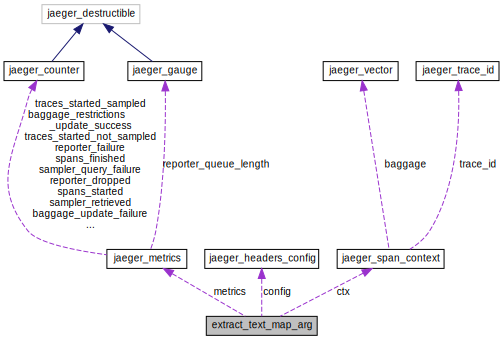
\includegraphics[width=350pt]{structextract__text__map__arg__coll__graph}
\end{center}
\end{figure}
\subsection*{Data Fields}
\begin{DoxyCompactItemize}
\item 
\mbox{\Hypertarget{structextract__text__map__arg_ab33860ffded14af993fee96f5d61cd6f}\label{structextract__text__map__arg_ab33860ffded14af993fee96f5d61cd6f}} 
\mbox{\hyperlink{structjaeger__span__context}{jaeger\+\_\+span\+\_\+context}} $\ast$ {\bfseries ctx}
\item 
\mbox{\Hypertarget{structextract__text__map__arg_a8d7e24ae1b3ae598b01d9e38e78fd002}\label{structextract__text__map__arg_a8d7e24ae1b3ae598b01d9e38e78fd002}} 
\mbox{\hyperlink{structjaeger__metrics}{jaeger\+\_\+metrics}} $\ast$ {\bfseries metrics}
\item 
\mbox{\Hypertarget{structextract__text__map__arg_aa06ff45434635affaff6e18a9d016e1e}\label{structextract__text__map__arg_aa06ff45434635affaff6e18a9d016e1e}} 
const \mbox{\hyperlink{structjaeger__headers__config}{jaeger\+\_\+headers\+\_\+config}} $\ast$ {\bfseries config}
\item 
\mbox{\Hypertarget{structextract__text__map__arg_ad66d013a675a98ad4744a26c84971355}\label{structextract__text__map__arg_ad66d013a675a98ad4744a26c84971355}} 
void($\ast$ {\bfseries normalize\+\_\+key} )(char $\ast$restrict, const char $\ast$restrict)
\item 
\mbox{\Hypertarget{structextract__text__map__arg_ac93640eecdaf124320f4e9fc975970f6}\label{structextract__text__map__arg_ac93640eecdaf124320f4e9fc975970f6}} 
void($\ast$ {\bfseries decode\+\_\+value} )(char $\ast$restrict, const char $\ast$restrict)
\end{DoxyCompactItemize}


The documentation for this struct was generated from the following file\+:\begin{DoxyCompactItemize}
\item 
jaegertracingc/\mbox{\hyperlink{propagation_8c}{propagation.\+c}}\end{DoxyCompactItemize}

\hypertarget{structjaeger__adaptive__sampler}{}\section{jaeger\+\_\+adaptive\+\_\+sampler Struct Reference}
\label{structjaeger__adaptive__sampler}\index{jaeger\+\_\+adaptive\+\_\+sampler@{jaeger\+\_\+adaptive\+\_\+sampler}}


Collaboration diagram for jaeger\+\_\+adaptive\+\_\+sampler\+:\nopagebreak
\begin{figure}[H]
\begin{center}
\leavevmode
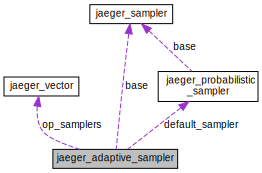
\includegraphics[width=335pt]{structjaeger__adaptive__sampler__coll__graph}
\end{center}
\end{figure}
\subsection*{Data Fields}
\begin{DoxyCompactItemize}
\item 
\mbox{\Hypertarget{structjaeger__adaptive__sampler_aaa0f3aaf48e84c9c47258009980bc2ac}\label{structjaeger__adaptive__sampler_aaa0f3aaf48e84c9c47258009980bc2ac}} 
\mbox{\hyperlink{structjaeger__sampler}{jaeger\+\_\+sampler}} {\bfseries base}
\item 
\mbox{\Hypertarget{structjaeger__adaptive__sampler_a51357b8b680e9658d185b2a5fcee0ca0}\label{structjaeger__adaptive__sampler_a51357b8b680e9658d185b2a5fcee0ca0}} 
\mbox{\hyperlink{structjaeger__vector}{jaeger\+\_\+vector}} {\bfseries op\+\_\+samplers}
\item 
\mbox{\Hypertarget{structjaeger__adaptive__sampler_a4bbda4f0edbb4d3e1f3c7633ab208af3}\label{structjaeger__adaptive__sampler_a4bbda4f0edbb4d3e1f3c7633ab208af3}} 
\mbox{\hyperlink{structjaeger__probabilistic__sampler}{jaeger\+\_\+probabilistic\+\_\+sampler}} {\bfseries default\+\_\+sampler}
\item 
\mbox{\Hypertarget{structjaeger__adaptive__sampler_aaf614c9bb539c04d7700f236e905c8f3}\label{structjaeger__adaptive__sampler_aaf614c9bb539c04d7700f236e905c8f3}} 
double {\bfseries lower\+\_\+bound}
\item 
\mbox{\Hypertarget{structjaeger__adaptive__sampler_af3ea970b95f9c506486da7ef8a6e9e8e}\label{structjaeger__adaptive__sampler_af3ea970b95f9c506486da7ef8a6e9e8e}} 
int {\bfseries max\+\_\+operations}
\item 
\mbox{\Hypertarget{structjaeger__adaptive__sampler_a42730aa12aabed22ac323d79b1650b6d}\label{structjaeger__adaptive__sampler_a42730aa12aabed22ac323d79b1650b6d}} 
jaeger\+\_\+mutex {\bfseries mutex}
\end{DoxyCompactItemize}


The documentation for this struct was generated from the following file\+:\begin{DoxyCompactItemize}
\item 
jaegertracingc/\mbox{\hyperlink{sampler_8h}{sampler.\+h}}\end{DoxyCompactItemize}

\hypertarget{structjaeger__allocator}{}\section{jaeger\+\_\+allocator Struct Reference}
\label{structjaeger__allocator}\index{jaeger\+\_\+allocator@{jaeger\+\_\+allocator}}


Interface to override default allocator.  




{\ttfamily \#include $<$jaegertracingc/alloc.\+h$>$}

\subsection*{Data Fields}
\begin{DoxyCompactItemize}
\item 
void $\ast$($\ast$ \mbox{\hyperlink{structjaeger__allocator_a235caded5cb561736c69c28b47169864}{malloc}} )(struct \mbox{\hyperlink{structjaeger__allocator}{jaeger\+\_\+allocator}} $\ast$alloc, size\+\_\+t sz)
\begin{DoxyCompactList}\small\item\em malloc function override. \end{DoxyCompactList}\item 
void $\ast$($\ast$ \mbox{\hyperlink{structjaeger__allocator_a17a8373babb00b98a1303cafaf524676}{realloc}} )(struct \mbox{\hyperlink{structjaeger__allocator}{jaeger\+\_\+allocator}} $\ast$alloc, void $\ast$ptr, size\+\_\+t sz)
\begin{DoxyCompactList}\small\item\em realloc function override. \end{DoxyCompactList}\item 
void($\ast$ \mbox{\hyperlink{structjaeger__allocator_a740ff44da0e720a728593e26bf58acc4}{free}} )(struct \mbox{\hyperlink{structjaeger__allocator}{jaeger\+\_\+allocator}} $\ast$alloc, void $\ast$ptr)
\begin{DoxyCompactList}\small\item\em free function override. \end{DoxyCompactList}\end{DoxyCompactItemize}


\subsection{Detailed Description}
Interface to override default allocator. 



\subsection{Field Documentation}
\mbox{\Hypertarget{structjaeger__allocator_a740ff44da0e720a728593e26bf58acc4}\label{structjaeger__allocator_a740ff44da0e720a728593e26bf58acc4}} 
\index{jaeger\+\_\+allocator@{jaeger\+\_\+allocator}!free@{free}}
\index{free@{free}!jaeger\+\_\+allocator@{jaeger\+\_\+allocator}}
\subsubsection{\texorpdfstring{free}{free}}
{\footnotesize\ttfamily void($\ast$ jaeger\+\_\+allocator\+::free) (struct \mbox{\hyperlink{structjaeger__allocator}{jaeger\+\_\+allocator}} $\ast$alloc, void $\ast$ptr)}



free function override. 


\begin{DoxyParams}{Parameters}
{\em alloc} & Allocator instance. \\
\hline
{\em ptr} & Pointer to he allocated memory to free. \\
\hline
\end{DoxyParams}
\mbox{\Hypertarget{structjaeger__allocator_a235caded5cb561736c69c28b47169864}\label{structjaeger__allocator_a235caded5cb561736c69c28b47169864}} 
\index{jaeger\+\_\+allocator@{jaeger\+\_\+allocator}!malloc@{malloc}}
\index{malloc@{malloc}!jaeger\+\_\+allocator@{jaeger\+\_\+allocator}}
\subsubsection{\texorpdfstring{malloc}{malloc}}
{\footnotesize\ttfamily void$\ast$($\ast$ jaeger\+\_\+allocator\+::malloc) (struct \mbox{\hyperlink{structjaeger__allocator}{jaeger\+\_\+allocator}} $\ast$alloc, size\+\_\+t sz)}



malloc function override. 


\begin{DoxyParams}{Parameters}
{\em alloc} & Allocator instance. \\
\hline
{\em sz} & Size to allocate. \\
\hline
\end{DoxyParams}
\begin{DoxyReturn}{Returns}
Pointer to allocated memory on success, N\+U\+LL otherwise. 
\end{DoxyReturn}
\mbox{\Hypertarget{structjaeger__allocator_a17a8373babb00b98a1303cafaf524676}\label{structjaeger__allocator_a17a8373babb00b98a1303cafaf524676}} 
\index{jaeger\+\_\+allocator@{jaeger\+\_\+allocator}!realloc@{realloc}}
\index{realloc@{realloc}!jaeger\+\_\+allocator@{jaeger\+\_\+allocator}}
\subsubsection{\texorpdfstring{realloc}{realloc}}
{\footnotesize\ttfamily void$\ast$($\ast$ jaeger\+\_\+allocator\+::realloc) (struct \mbox{\hyperlink{structjaeger__allocator}{jaeger\+\_\+allocator}} $\ast$alloc, void $\ast$ptr, size\+\_\+t sz)}



realloc function override. 


\begin{DoxyParams}{Parameters}
{\em alloc} & Allocator instance. \\
\hline
{\em ptr} & Pointer to previously allocated memory. \\
\hline
{\em sz} & New size to allocate. \\
\hline
\end{DoxyParams}
\begin{DoxyReturn}{Returns}
Pointer to new allocated memory on success, N\+U\+LL otherwise. 
\end{DoxyReturn}


The documentation for this struct was generated from the following file\+:\begin{DoxyCompactItemize}
\item 
jaegertracingc/\mbox{\hyperlink{alloc_8h}{alloc.\+h}}\end{DoxyCompactItemize}

\hypertarget{structjaeger__baggage__restriction}{}\section{jaeger\+\_\+baggage\+\_\+restriction Struct Reference}
\label{structjaeger__baggage__restriction}\index{jaeger\+\_\+baggage\+\_\+restriction@{jaeger\+\_\+baggage\+\_\+restriction}}


Representation of baggage restriction for a given key and a given service.  




{\ttfamily \#include $<$jaegertracingc/baggage.\+h$>$}

\subsection*{Data Fields}
\begin{DoxyCompactItemize}
\item 
bool \mbox{\hyperlink{structjaeger__baggage__restriction_a0adda71667eefac438221ea727c5f1be}{key\+\_\+allowed}}
\begin{DoxyCompactList}\small\item\em Whether or not the key is allowed at all. \end{DoxyCompactList}\item 
size\+\_\+t \mbox{\hyperlink{structjaeger__baggage__restriction_a740265dd2c887da97c9682ae6b5be73d}{max\+\_\+value\+\_\+len}}
\begin{DoxyCompactList}\small\item\em Maximum value length for the given key. \end{DoxyCompactList}\end{DoxyCompactItemize}


\subsection{Detailed Description}
Representation of baggage restriction for a given key and a given service. 

\subsection{Field Documentation}
\mbox{\Hypertarget{structjaeger__baggage__restriction_a0adda71667eefac438221ea727c5f1be}\label{structjaeger__baggage__restriction_a0adda71667eefac438221ea727c5f1be}} 
\index{jaeger\+\_\+baggage\+\_\+restriction@{jaeger\+\_\+baggage\+\_\+restriction}!key\+\_\+allowed@{key\+\_\+allowed}}
\index{key\+\_\+allowed@{key\+\_\+allowed}!jaeger\+\_\+baggage\+\_\+restriction@{jaeger\+\_\+baggage\+\_\+restriction}}
\subsubsection{\texorpdfstring{key\+\_\+allowed}{key\_allowed}}
{\footnotesize\ttfamily bool jaeger\+\_\+baggage\+\_\+restriction\+::key\+\_\+allowed}



Whether or not the key is allowed at all. 

\mbox{\Hypertarget{structjaeger__baggage__restriction_a740265dd2c887da97c9682ae6b5be73d}\label{structjaeger__baggage__restriction_a740265dd2c887da97c9682ae6b5be73d}} 
\index{jaeger\+\_\+baggage\+\_\+restriction@{jaeger\+\_\+baggage\+\_\+restriction}!max\+\_\+value\+\_\+len@{max\+\_\+value\+\_\+len}}
\index{max\+\_\+value\+\_\+len@{max\+\_\+value\+\_\+len}!jaeger\+\_\+baggage\+\_\+restriction@{jaeger\+\_\+baggage\+\_\+restriction}}
\subsubsection{\texorpdfstring{max\+\_\+value\+\_\+len}{max\_value\_len}}
{\footnotesize\ttfamily size\+\_\+t jaeger\+\_\+baggage\+\_\+restriction\+::max\+\_\+value\+\_\+len}



Maximum value length for the given key. 



The documentation for this struct was generated from the following file\+:\begin{DoxyCompactItemize}
\item 
jaegertracingc/\mbox{\hyperlink{baggage_8h}{baggage.\+h}}\end{DoxyCompactItemize}

\hypertarget{structjaeger__baggage__restriction__manager}{}\section{jaeger\+\_\+baggage\+\_\+restriction\+\_\+manager Struct Reference}
\label{structjaeger__baggage__restriction__manager}\index{jaeger\+\_\+baggage\+\_\+restriction\+\_\+manager@{jaeger\+\_\+baggage\+\_\+restriction\+\_\+manager}}


Interface for object that manages baggage restrictions.  




{\ttfamily \#include $<$jaegertracingc/baggage.\+h$>$}



Inheritance diagram for jaeger\+\_\+baggage\+\_\+restriction\+\_\+manager\+:\nopagebreak
\begin{figure}[H]
\begin{center}
\leavevmode
\includegraphics[width=213pt]{structjaeger__baggage__restriction__manager__inherit__graph}
\end{center}
\end{figure}


Collaboration diagram for jaeger\+\_\+baggage\+\_\+restriction\+\_\+manager\+:\nopagebreak
\begin{figure}[H]
\begin{center}
\leavevmode
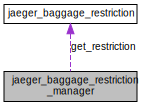
\includegraphics[width=213pt]{structjaeger__baggage__restriction__manager__coll__graph}
\end{center}
\end{figure}
\subsection*{Data Fields}
\begin{DoxyCompactItemize}
\item 
\mbox{\hyperlink{structjaeger__baggage__restriction}{jaeger\+\_\+baggage\+\_\+restriction}}($\ast$ \mbox{\hyperlink{structjaeger__baggage__restriction__manager_a1b451e0b12cecf51714f8760831fcc40}{get\+\_\+restriction}} )(struct \mbox{\hyperlink{structjaeger__baggage__restriction__manager}{jaeger\+\_\+baggage\+\_\+restriction\+\_\+manager}} $\ast$manager, const char $\ast$service, const char $\ast$key)
\begin{DoxyCompactList}\small\item\em Get restriction regarding a given key for a given service. \end{DoxyCompactList}\end{DoxyCompactItemize}


\subsection{Detailed Description}
Interface for object that manages baggage restrictions. 

\subsection{Field Documentation}
\mbox{\Hypertarget{structjaeger__baggage__restriction__manager_a1b451e0b12cecf51714f8760831fcc40}\label{structjaeger__baggage__restriction__manager_a1b451e0b12cecf51714f8760831fcc40}} 
\index{jaeger\+\_\+baggage\+\_\+restriction\+\_\+manager@{jaeger\+\_\+baggage\+\_\+restriction\+\_\+manager}!get\+\_\+restriction@{get\+\_\+restriction}}
\index{get\+\_\+restriction@{get\+\_\+restriction}!jaeger\+\_\+baggage\+\_\+restriction\+\_\+manager@{jaeger\+\_\+baggage\+\_\+restriction\+\_\+manager}}
\subsubsection{\texorpdfstring{get\+\_\+restriction}{get\_restriction}}
{\footnotesize\ttfamily \mbox{\hyperlink{structjaeger__baggage__restriction}{jaeger\+\_\+baggage\+\_\+restriction}}($\ast$ jaeger\+\_\+baggage\+\_\+restriction\+\_\+manager\+::get\+\_\+restriction) (struct \mbox{\hyperlink{structjaeger__baggage__restriction__manager}{jaeger\+\_\+baggage\+\_\+restriction\+\_\+manager}} $\ast$manager, const char $\ast$service, const char $\ast$key)}



Get restriction regarding a given key for a given service. 


\begin{DoxyParams}{Parameters}
{\em manager} & Manager instance. \\
\hline
{\em service} & Service name. \\
\hline
{\em key} & Baggage key. \\
\hline
\end{DoxyParams}
\begin{DoxyReturn}{Returns}
Baggage restriction value. 
\end{DoxyReturn}


The documentation for this struct was generated from the following file\+:\begin{DoxyCompactItemize}
\item 
jaegertracingc/\mbox{\hyperlink{baggage_8h}{baggage.\+h}}\end{DoxyCompactItemize}

\hypertarget{structjaeger__baggage__restrictions__config}{}\section{jaeger\+\_\+baggage\+\_\+restrictions\+\_\+config Struct Reference}
\label{structjaeger__baggage__restrictions__config}\index{jaeger\+\_\+baggage\+\_\+restrictions\+\_\+config@{jaeger\+\_\+baggage\+\_\+restrictions\+\_\+config}}


Baggage restrictions config.  




{\ttfamily \#include $<$jaegertracingc/options.\+h$>$}



\subsection{Detailed Description}
Baggage restrictions config. 



The documentation for this struct was generated from the following file\+:\begin{DoxyCompactItemize}
\item 
jaegertracingc/\mbox{\hyperlink{options_8h}{options.\+h}}\end{DoxyCompactItemize}

\hypertarget{structjaeger__baggage__setter}{}\section{jaeger\+\_\+baggage\+\_\+setter Struct Reference}
\label{structjaeger__baggage__setter}\index{jaeger\+\_\+baggage\+\_\+setter@{jaeger\+\_\+baggage\+\_\+setter}}


Facade to enforce remote baggage restrictions in tracer.  




{\ttfamily \#include $<$jaegertracingc/baggage.\+h$>$}



Collaboration diagram for jaeger\+\_\+baggage\+\_\+setter\+:\nopagebreak
\begin{figure}[H]
\begin{center}
\leavevmode
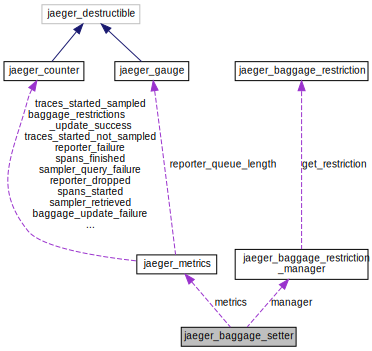
\includegraphics[width=350pt]{structjaeger__baggage__setter__coll__graph}
\end{center}
\end{figure}
\subsection*{Data Fields}
\begin{DoxyCompactItemize}
\item 
\mbox{\hyperlink{structjaeger__baggage__restriction__manager}{jaeger\+\_\+baggage\+\_\+restriction\+\_\+manager}} $\ast$ \mbox{\hyperlink{structjaeger__baggage__setter_ae0278c0f8980fa770fadcbe9fa82d507}{manager}}
\begin{DoxyCompactList}\small\item\em Remote baggage restriction manager instance. \end{DoxyCompactList}\item 
\mbox{\hyperlink{structjaeger__metrics}{jaeger\+\_\+metrics}} $\ast$ \mbox{\hyperlink{structjaeger__baggage__setter_a0ed0b61f9d103eda5775cbcfc200c802}{metrics}}
\begin{DoxyCompactList}\small\item\em Metrics used for maintaining success count, error count, etc. \end{DoxyCompactList}\end{DoxyCompactItemize}


\subsection{Detailed Description}
Facade to enforce remote baggage restrictions in tracer. 



\subsection{Field Documentation}
\mbox{\Hypertarget{structjaeger__baggage__setter_ae0278c0f8980fa770fadcbe9fa82d507}\label{structjaeger__baggage__setter_ae0278c0f8980fa770fadcbe9fa82d507}} 
\index{jaeger\+\_\+baggage\+\_\+setter@{jaeger\+\_\+baggage\+\_\+setter}!manager@{manager}}
\index{manager@{manager}!jaeger\+\_\+baggage\+\_\+setter@{jaeger\+\_\+baggage\+\_\+setter}}
\subsubsection{\texorpdfstring{manager}{manager}}
{\footnotesize\ttfamily \mbox{\hyperlink{structjaeger__baggage__restriction__manager}{jaeger\+\_\+baggage\+\_\+restriction\+\_\+manager}}$\ast$ jaeger\+\_\+baggage\+\_\+setter\+::manager}



Remote baggage restriction manager instance. 

\mbox{\Hypertarget{structjaeger__baggage__setter_a0ed0b61f9d103eda5775cbcfc200c802}\label{structjaeger__baggage__setter_a0ed0b61f9d103eda5775cbcfc200c802}} 
\index{jaeger\+\_\+baggage\+\_\+setter@{jaeger\+\_\+baggage\+\_\+setter}!metrics@{metrics}}
\index{metrics@{metrics}!jaeger\+\_\+baggage\+\_\+setter@{jaeger\+\_\+baggage\+\_\+setter}}
\subsubsection{\texorpdfstring{metrics}{metrics}}
{\footnotesize\ttfamily \mbox{\hyperlink{structjaeger__metrics}{jaeger\+\_\+metrics}}$\ast$ jaeger\+\_\+baggage\+\_\+setter\+::metrics}



Metrics used for maintaining success count, error count, etc. 



The documentation for this struct was generated from the following file\+:\begin{DoxyCompactItemize}
\item 
jaegertracingc/\mbox{\hyperlink{baggage_8h}{baggage.\+h}}\end{DoxyCompactItemize}

\hypertarget{structjaeger__composite__reporter}{}\section{jaeger\+\_\+composite\+\_\+reporter Struct Reference}
\label{structjaeger__composite__reporter}\index{jaeger\+\_\+composite\+\_\+reporter@{jaeger\+\_\+composite\+\_\+reporter}}


Collaboration diagram for jaeger\+\_\+composite\+\_\+reporter\+:\nopagebreak
\begin{figure}[H]
\begin{center}
\leavevmode
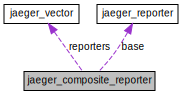
\includegraphics[width=254pt]{structjaeger__composite__reporter__coll__graph}
\end{center}
\end{figure}
\subsection*{Data Fields}
\begin{DoxyCompactItemize}
\item 
\mbox{\Hypertarget{structjaeger__composite__reporter_a453a9d8f7687b566527162f37af62db6}\label{structjaeger__composite__reporter_a453a9d8f7687b566527162f37af62db6}} 
\mbox{\hyperlink{structjaeger__reporter}{jaeger\+\_\+reporter}} {\bfseries base}
\item 
\mbox{\Hypertarget{structjaeger__composite__reporter_a47166572f9bcadee17edf3a73a6d6311}\label{structjaeger__composite__reporter_a47166572f9bcadee17edf3a73a6d6311}} 
\mbox{\hyperlink{structjaeger__vector}{jaeger\+\_\+vector}} {\bfseries reporters}
\end{DoxyCompactItemize}


The documentation for this struct was generated from the following file\+:\begin{DoxyCompactItemize}
\item 
jaegertracingc/\mbox{\hyperlink{reporter_8h}{reporter.\+h}}\end{DoxyCompactItemize}

\hypertarget{structjaeger__config}{}\section{jaeger\+\_\+config Struct Reference}
\label{structjaeger__config}\index{jaeger\+\_\+config@{jaeger\+\_\+config}}


Overall Jaeger configuration object.  




{\ttfamily \#include $<$jaegertracingc/options.\+h$>$}



Collaboration diagram for jaeger\+\_\+config\+:\nopagebreak
\begin{figure}[H]
\begin{center}
\leavevmode
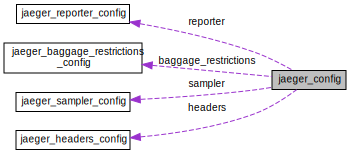
\includegraphics[width=350pt]{structjaeger__config__coll__graph}
\end{center}
\end{figure}
\subsection*{Data Fields}
\begin{DoxyCompactItemize}
\item 
bool \mbox{\hyperlink{structjaeger__config_a3edfc4072b15da75a19efb85ea781726}{disabled}}
\begin{DoxyCompactList}\small\item\em Flag to disable tracing. \end{DoxyCompactList}\item 
\mbox{\hyperlink{structjaeger__sampler__config}{jaeger\+\_\+sampler\+\_\+config}} \mbox{\hyperlink{structjaeger__config_a812f67f2637466de160309af68951713}{sampler}}
\begin{DoxyCompactList}\small\item\em Sampler config. \end{DoxyCompactList}\item 
\mbox{\hyperlink{structjaeger__reporter__config}{jaeger\+\_\+reporter\+\_\+config}} \mbox{\hyperlink{structjaeger__config_a5bd07c1b0274f5026ccafd4bbc7260c7}{reporter}}
\begin{DoxyCompactList}\small\item\em Reporter config. \end{DoxyCompactList}\item 
\mbox{\hyperlink{structjaeger__headers__config}{jaeger\+\_\+headers\+\_\+config}} \mbox{\hyperlink{structjaeger__config_a200401ea8b4175a4888dcb1d296ef73d}{headers}}
\begin{DoxyCompactList}\small\item\em Headers config. \end{DoxyCompactList}\item 
\mbox{\hyperlink{structjaeger__baggage__restrictions__config}{jaeger\+\_\+baggage\+\_\+restrictions\+\_\+config}} \mbox{\hyperlink{structjaeger__config_a33fd9cfa26f4b54cb9a7abfd405f2723}{baggage\+\_\+restrictions}}
\begin{DoxyCompactList}\small\item\em Baggage restrictions config. \end{DoxyCompactList}\end{DoxyCompactItemize}


\subsection{Detailed Description}
Overall Jaeger configuration object. 



\subsection{Field Documentation}
\mbox{\Hypertarget{structjaeger__config_a33fd9cfa26f4b54cb9a7abfd405f2723}\label{structjaeger__config_a33fd9cfa26f4b54cb9a7abfd405f2723}} 
\index{jaeger\+\_\+config@{jaeger\+\_\+config}!baggage\+\_\+restrictions@{baggage\+\_\+restrictions}}
\index{baggage\+\_\+restrictions@{baggage\+\_\+restrictions}!jaeger\+\_\+config@{jaeger\+\_\+config}}
\subsubsection{\texorpdfstring{baggage\+\_\+restrictions}{baggage\_restrictions}}
{\footnotesize\ttfamily \mbox{\hyperlink{structjaeger__baggage__restrictions__config}{jaeger\+\_\+baggage\+\_\+restrictions\+\_\+config}} jaeger\+\_\+config\+::baggage\+\_\+restrictions}



Baggage restrictions config. 

\mbox{\Hypertarget{structjaeger__config_a3edfc4072b15da75a19efb85ea781726}\label{structjaeger__config_a3edfc4072b15da75a19efb85ea781726}} 
\index{jaeger\+\_\+config@{jaeger\+\_\+config}!disabled@{disabled}}
\index{disabled@{disabled}!jaeger\+\_\+config@{jaeger\+\_\+config}}
\subsubsection{\texorpdfstring{disabled}{disabled}}
{\footnotesize\ttfamily bool jaeger\+\_\+config\+::disabled}



Flag to disable tracing. 

\mbox{\Hypertarget{structjaeger__config_a200401ea8b4175a4888dcb1d296ef73d}\label{structjaeger__config_a200401ea8b4175a4888dcb1d296ef73d}} 
\index{jaeger\+\_\+config@{jaeger\+\_\+config}!headers@{headers}}
\index{headers@{headers}!jaeger\+\_\+config@{jaeger\+\_\+config}}
\subsubsection{\texorpdfstring{headers}{headers}}
{\footnotesize\ttfamily \mbox{\hyperlink{structjaeger__headers__config}{jaeger\+\_\+headers\+\_\+config}} jaeger\+\_\+config\+::headers}



Headers config. 

\mbox{\Hypertarget{structjaeger__config_a5bd07c1b0274f5026ccafd4bbc7260c7}\label{structjaeger__config_a5bd07c1b0274f5026ccafd4bbc7260c7}} 
\index{jaeger\+\_\+config@{jaeger\+\_\+config}!reporter@{reporter}}
\index{reporter@{reporter}!jaeger\+\_\+config@{jaeger\+\_\+config}}
\subsubsection{\texorpdfstring{reporter}{reporter}}
{\footnotesize\ttfamily \mbox{\hyperlink{structjaeger__reporter__config}{jaeger\+\_\+reporter\+\_\+config}} jaeger\+\_\+config\+::reporter}



Reporter config. 

\mbox{\Hypertarget{structjaeger__config_a812f67f2637466de160309af68951713}\label{structjaeger__config_a812f67f2637466de160309af68951713}} 
\index{jaeger\+\_\+config@{jaeger\+\_\+config}!sampler@{sampler}}
\index{sampler@{sampler}!jaeger\+\_\+config@{jaeger\+\_\+config}}
\subsubsection{\texorpdfstring{sampler}{sampler}}
{\footnotesize\ttfamily \mbox{\hyperlink{structjaeger__sampler__config}{jaeger\+\_\+sampler\+\_\+config}} jaeger\+\_\+config\+::sampler}



Sampler config. 



The documentation for this struct was generated from the following file\+:\begin{DoxyCompactItemize}
\item 
jaegertracingc/\mbox{\hyperlink{options_8h}{options.\+h}}\end{DoxyCompactItemize}

\hypertarget{structjaeger__const__sampler}{}\section{jaeger\+\_\+const\+\_\+sampler Struct Reference}
\label{structjaeger__const__sampler}\index{jaeger\+\_\+const\+\_\+sampler@{jaeger\+\_\+const\+\_\+sampler}}


Collaboration diagram for jaeger\+\_\+const\+\_\+sampler\+:\nopagebreak
\begin{figure}[H]
\begin{center}
\leavevmode
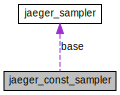
\includegraphics[width=192pt]{structjaeger__const__sampler__coll__graph}
\end{center}
\end{figure}
\subsection*{Data Fields}
\begin{DoxyCompactItemize}
\item 
\mbox{\Hypertarget{structjaeger__const__sampler_a1346f1dc941bcd9eed5f790d4ab3d9e9}\label{structjaeger__const__sampler_a1346f1dc941bcd9eed5f790d4ab3d9e9}} 
\mbox{\hyperlink{structjaeger__sampler}{jaeger\+\_\+sampler}} {\bfseries base}
\item 
\mbox{\Hypertarget{structjaeger__const__sampler_a6505c6a75f08c99b9c786e142bee3d41}\label{structjaeger__const__sampler_a6505c6a75f08c99b9c786e142bee3d41}} 
bool {\bfseries decision}
\end{DoxyCompactItemize}


The documentation for this struct was generated from the following file\+:\begin{DoxyCompactItemize}
\item 
jaegertracingc/\mbox{\hyperlink{sampler_8h}{sampler.\+h}}\end{DoxyCompactItemize}

\hypertarget{structjaeger__counter}{}\section{jaeger\+\_\+counter Struct Reference}
\label{structjaeger__counter}\index{jaeger\+\_\+counter@{jaeger\+\_\+counter}}


Counter metric interface.  




{\ttfamily \#include $<$jaegertracingc/metrics.\+h$>$}



Inheritance diagram for jaeger\+\_\+counter\+:\nopagebreak
\begin{figure}[H]
\begin{center}
\leavevmode
\includegraphics[width=178pt]{structjaeger__counter__inherit__graph}
\end{center}
\end{figure}


Collaboration diagram for jaeger\+\_\+counter\+:\nopagebreak
\begin{figure}[H]
\begin{center}
\leavevmode
\includegraphics[width=178pt]{structjaeger__counter__coll__graph}
\end{center}
\end{figure}
\subsection*{Data Fields}
\begin{DoxyCompactItemize}
\item 
jaeger\+\_\+destructible \mbox{\hyperlink{structjaeger__counter_abc889348825fd450db8b207dbfb17777}{base}}
\begin{DoxyCompactList}\small\item\em Base class member. \end{DoxyCompactList}\item 
void($\ast$ \mbox{\hyperlink{structjaeger__counter_a349dc48bc8872abe4b73246c8be49aca}{inc}} )(struct \mbox{\hyperlink{structjaeger__counter}{jaeger\+\_\+counter}} $\ast$counter, int64\+\_\+t delta)
\begin{DoxyCompactList}\small\item\em Increment count. \end{DoxyCompactList}\end{DoxyCompactItemize}


\subsection{Detailed Description}
Counter metric interface. 

Counters are used to keep track of a total number of events (i.\+e. number of spans reported). 

\subsection{Field Documentation}
\mbox{\Hypertarget{structjaeger__counter_abc889348825fd450db8b207dbfb17777}\label{structjaeger__counter_abc889348825fd450db8b207dbfb17777}} 
\index{jaeger\+\_\+counter@{jaeger\+\_\+counter}!base@{base}}
\index{base@{base}!jaeger\+\_\+counter@{jaeger\+\_\+counter}}
\subsubsection{\texorpdfstring{base}{base}}
{\footnotesize\ttfamily jaeger\+\_\+destructible jaeger\+\_\+counter\+::base}



Base class member. 

\mbox{\Hypertarget{structjaeger__counter_a349dc48bc8872abe4b73246c8be49aca}\label{structjaeger__counter_a349dc48bc8872abe4b73246c8be49aca}} 
\index{jaeger\+\_\+counter@{jaeger\+\_\+counter}!inc@{inc}}
\index{inc@{inc}!jaeger\+\_\+counter@{jaeger\+\_\+counter}}
\subsubsection{\texorpdfstring{inc}{inc}}
{\footnotesize\ttfamily void($\ast$ jaeger\+\_\+counter\+::inc) (struct \mbox{\hyperlink{structjaeger__counter}{jaeger\+\_\+counter}} $\ast$counter, int64\+\_\+t delta)}



Increment count. 


\begin{DoxyParams}{Parameters}
{\em counter} & Counter to increment. \\
\hline
{\em delta} & Amount to increment. \\
\hline
\end{DoxyParams}


The documentation for this struct was generated from the following file\+:\begin{DoxyCompactItemize}
\item 
jaegertracingc/\mbox{\hyperlink{metrics_8h}{metrics.\+h}}\end{DoxyCompactItemize}

\hypertarget{structjaeger__default__baggage__restriction__manager}{}\section{jaeger\+\_\+default\+\_\+baggage\+\_\+restriction\+\_\+manager Struct Reference}
\label{structjaeger__default__baggage__restriction__manager}\index{jaeger\+\_\+default\+\_\+baggage\+\_\+restriction\+\_\+manager@{jaeger\+\_\+default\+\_\+baggage\+\_\+restriction\+\_\+manager}}


Default implementation of \mbox{\hyperlink{structjaeger__baggage__restriction__manager}{jaeger\+\_\+baggage\+\_\+restriction\+\_\+manager}} interface.  




{\ttfamily \#include $<$jaegertracingc/baggage.\+h$>$}



Inheritance diagram for jaeger\+\_\+default\+\_\+baggage\+\_\+restriction\+\_\+manager\+:\nopagebreak
\begin{figure}[H]
\begin{center}
\leavevmode
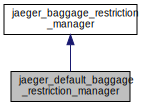
\includegraphics[width=213pt]{structjaeger__default__baggage__restriction__manager__inherit__graph}
\end{center}
\end{figure}


Collaboration diagram for jaeger\+\_\+default\+\_\+baggage\+\_\+restriction\+\_\+manager\+:\nopagebreak
\begin{figure}[H]
\begin{center}
\leavevmode
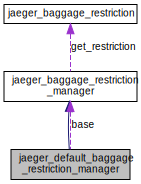
\includegraphics[width=213pt]{structjaeger__default__baggage__restriction__manager__coll__graph}
\end{center}
\end{figure}
\subsection*{Data Fields}
\begin{DoxyCompactItemize}
\item 
\mbox{\hyperlink{structjaeger__baggage__restriction__manager}{jaeger\+\_\+baggage\+\_\+restriction\+\_\+manager}} \mbox{\hyperlink{structjaeger__default__baggage__restriction__manager_a6a99e5ce74dcbc815354e6d37648f834}{base}}
\begin{DoxyCompactList}\small\item\em Base class instance. \end{DoxyCompactList}\item 
size\+\_\+t \mbox{\hyperlink{structjaeger__default__baggage__restriction__manager_acfc66e81601e92bb3ef1b43ceca9fc19}{max\+\_\+value\+\_\+len}}
\begin{DoxyCompactList}\small\item\em Maximum value length for every key. \end{DoxyCompactList}\end{DoxyCompactItemize}


\subsection{Detailed Description}
Default implementation of \mbox{\hyperlink{structjaeger__baggage__restriction__manager}{jaeger\+\_\+baggage\+\_\+restriction\+\_\+manager}} interface. 

\subsection{Field Documentation}
\mbox{\Hypertarget{structjaeger__default__baggage__restriction__manager_a6a99e5ce74dcbc815354e6d37648f834}\label{structjaeger__default__baggage__restriction__manager_a6a99e5ce74dcbc815354e6d37648f834}} 
\index{jaeger\+\_\+default\+\_\+baggage\+\_\+restriction\+\_\+manager@{jaeger\+\_\+default\+\_\+baggage\+\_\+restriction\+\_\+manager}!base@{base}}
\index{base@{base}!jaeger\+\_\+default\+\_\+baggage\+\_\+restriction\+\_\+manager@{jaeger\+\_\+default\+\_\+baggage\+\_\+restriction\+\_\+manager}}
\subsubsection{\texorpdfstring{base}{base}}
{\footnotesize\ttfamily \mbox{\hyperlink{structjaeger__baggage__restriction__manager}{jaeger\+\_\+baggage\+\_\+restriction\+\_\+manager}} jaeger\+\_\+default\+\_\+baggage\+\_\+restriction\+\_\+manager\+::base}



Base class instance. 

\mbox{\Hypertarget{structjaeger__default__baggage__restriction__manager_acfc66e81601e92bb3ef1b43ceca9fc19}\label{structjaeger__default__baggage__restriction__manager_acfc66e81601e92bb3ef1b43ceca9fc19}} 
\index{jaeger\+\_\+default\+\_\+baggage\+\_\+restriction\+\_\+manager@{jaeger\+\_\+default\+\_\+baggage\+\_\+restriction\+\_\+manager}!max\+\_\+value\+\_\+len@{max\+\_\+value\+\_\+len}}
\index{max\+\_\+value\+\_\+len@{max\+\_\+value\+\_\+len}!jaeger\+\_\+default\+\_\+baggage\+\_\+restriction\+\_\+manager@{jaeger\+\_\+default\+\_\+baggage\+\_\+restriction\+\_\+manager}}
\subsubsection{\texorpdfstring{max\+\_\+value\+\_\+len}{max\_value\_len}}
{\footnotesize\ttfamily size\+\_\+t jaeger\+\_\+default\+\_\+baggage\+\_\+restriction\+\_\+manager\+::max\+\_\+value\+\_\+len}



Maximum value length for every key. 



The documentation for this struct was generated from the following file\+:\begin{DoxyCompactItemize}
\item 
jaegertracingc/\mbox{\hyperlink{baggage_8h}{baggage.\+h}}\end{DoxyCompactItemize}

\hypertarget{structjaeger__default__counter}{}\section{jaeger\+\_\+default\+\_\+counter Struct Reference}
\label{structjaeger__default__counter}\index{jaeger\+\_\+default\+\_\+counter@{jaeger\+\_\+default\+\_\+counter}}


Implements the counter interface with basic 64 bit integer value.  




{\ttfamily \#include $<$jaegertracingc/metrics.\+h$>$}



Collaboration diagram for jaeger\+\_\+default\+\_\+counter\+:\nopagebreak
\begin{figure}[H]
\begin{center}
\leavevmode
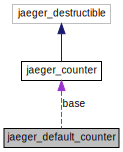
\includegraphics[width=195pt]{structjaeger__default__counter__coll__graph}
\end{center}
\end{figure}
\subsection*{Data Fields}
\begin{DoxyCompactItemize}
\item 
\mbox{\Hypertarget{structjaeger__default__counter_a1b29bf6888032ef2f05ee09fc67bd621}\label{structjaeger__default__counter_a1b29bf6888032ef2f05ee09fc67bd621}} 
\mbox{\hyperlink{structjaeger__counter}{jaeger\+\_\+counter}} {\bfseries base}
\item 
int64\+\_\+t \mbox{\hyperlink{structjaeger__default__counter_aaa90f254bc0b9720567642d2bb0422e8}{total}}
\begin{DoxyCompactList}\small\item\em Current total. \end{DoxyCompactList}\end{DoxyCompactItemize}


\subsection{Detailed Description}
Implements the counter interface with basic 64 bit integer value. 

\subsection{Field Documentation}
\mbox{\Hypertarget{structjaeger__default__counter_aaa90f254bc0b9720567642d2bb0422e8}\label{structjaeger__default__counter_aaa90f254bc0b9720567642d2bb0422e8}} 
\index{jaeger\+\_\+default\+\_\+counter@{jaeger\+\_\+default\+\_\+counter}!total@{total}}
\index{total@{total}!jaeger\+\_\+default\+\_\+counter@{jaeger\+\_\+default\+\_\+counter}}
\subsubsection{\texorpdfstring{total}{total}}
{\footnotesize\ttfamily int64\+\_\+t jaeger\+\_\+default\+\_\+counter\+::total}



Current total. 



The documentation for this struct was generated from the following file\+:\begin{DoxyCompactItemize}
\item 
jaegertracingc/\mbox{\hyperlink{metrics_8h}{metrics.\+h}}\end{DoxyCompactItemize}

\hypertarget{structjaeger__default__gauge}{}\section{jaeger\+\_\+default\+\_\+gauge Struct Reference}
\label{structjaeger__default__gauge}\index{jaeger\+\_\+default\+\_\+gauge@{jaeger\+\_\+default\+\_\+gauge}}


Implements gauge interface with basic 64 bit integer value.  




{\ttfamily \#include $<$jaegertracingc/metrics.\+h$>$}



Collaboration diagram for jaeger\+\_\+default\+\_\+gauge\+:\nopagebreak
\begin{figure}[H]
\begin{center}
\leavevmode
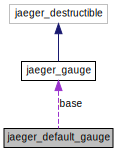
\includegraphics[width=189pt]{structjaeger__default__gauge__coll__graph}
\end{center}
\end{figure}
\subsection*{Data Fields}
\begin{DoxyCompactItemize}
\item 
\mbox{\Hypertarget{structjaeger__default__gauge_acef3ca538f119dac6856a6cfe65ca814}\label{structjaeger__default__gauge_acef3ca538f119dac6856a6cfe65ca814}} 
\mbox{\hyperlink{structjaeger__gauge}{jaeger\+\_\+gauge}} {\bfseries base}
\item 
int64\+\_\+t \mbox{\hyperlink{structjaeger__default__gauge_a5b5def7f03d492758487c564d9e0e6e3}{amount}}
\begin{DoxyCompactList}\small\item\em Current amount. \end{DoxyCompactList}\end{DoxyCompactItemize}


\subsection{Detailed Description}
Implements gauge interface with basic 64 bit integer value. 

\subsection{Field Documentation}
\mbox{\Hypertarget{structjaeger__default__gauge_a5b5def7f03d492758487c564d9e0e6e3}\label{structjaeger__default__gauge_a5b5def7f03d492758487c564d9e0e6e3}} 
\index{jaeger\+\_\+default\+\_\+gauge@{jaeger\+\_\+default\+\_\+gauge}!amount@{amount}}
\index{amount@{amount}!jaeger\+\_\+default\+\_\+gauge@{jaeger\+\_\+default\+\_\+gauge}}
\subsubsection{\texorpdfstring{amount}{amount}}
{\footnotesize\ttfamily int64\+\_\+t jaeger\+\_\+default\+\_\+gauge\+::amount}



Current amount. 



The documentation for this struct was generated from the following file\+:\begin{DoxyCompactItemize}
\item 
jaegertracingc/\mbox{\hyperlink{metrics_8h}{metrics.\+h}}\end{DoxyCompactItemize}

\hypertarget{structjaeger__gauge}{}\section{jaeger\+\_\+gauge Struct Reference}
\label{structjaeger__gauge}\index{jaeger\+\_\+gauge@{jaeger\+\_\+gauge}}


Gauge metric interface.  




{\ttfamily \#include $<$jaegertracingc/metrics.\+h$>$}



Inheritance diagram for jaeger\+\_\+gauge\+:\nopagebreak
\begin{figure}[H]
\begin{center}
\leavevmode
\includegraphics[width=178pt]{structjaeger__gauge__inherit__graph}
\end{center}
\end{figure}


Collaboration diagram for jaeger\+\_\+gauge\+:\nopagebreak
\begin{figure}[H]
\begin{center}
\leavevmode
\includegraphics[width=178pt]{structjaeger__gauge__coll__graph}
\end{center}
\end{figure}
\subsection*{Data Fields}
\begin{DoxyCompactItemize}
\item 
jaeger\+\_\+destructible \mbox{\hyperlink{structjaeger__gauge_a542160d18e7ee06a0ed466e4e0dfa9bd}{base}}
\begin{DoxyCompactList}\small\item\em Base class member. \end{DoxyCompactList}\item 
void($\ast$ \mbox{\hyperlink{structjaeger__gauge_a0463c13cf633754ea4cfe7588d1445a5}{update}} )(struct \mbox{\hyperlink{structjaeger__gauge}{jaeger\+\_\+gauge}} $\ast$gauge, int64\+\_\+t amount)
\begin{DoxyCompactList}\small\item\em Update current value of gauge. \end{DoxyCompactList}\end{DoxyCompactItemize}


\subsection{Detailed Description}
Gauge metric interface. 

Gauges are used to keep track of a changing number (i.\+e. number of items currently in a queue). 

\subsection{Field Documentation}
\mbox{\Hypertarget{structjaeger__gauge_a542160d18e7ee06a0ed466e4e0dfa9bd}\label{structjaeger__gauge_a542160d18e7ee06a0ed466e4e0dfa9bd}} 
\index{jaeger\+\_\+gauge@{jaeger\+\_\+gauge}!base@{base}}
\index{base@{base}!jaeger\+\_\+gauge@{jaeger\+\_\+gauge}}
\subsubsection{\texorpdfstring{base}{base}}
{\footnotesize\ttfamily jaeger\+\_\+destructible jaeger\+\_\+gauge\+::base}



Base class member. 

\mbox{\Hypertarget{structjaeger__gauge_a0463c13cf633754ea4cfe7588d1445a5}\label{structjaeger__gauge_a0463c13cf633754ea4cfe7588d1445a5}} 
\index{jaeger\+\_\+gauge@{jaeger\+\_\+gauge}!update@{update}}
\index{update@{update}!jaeger\+\_\+gauge@{jaeger\+\_\+gauge}}
\subsubsection{\texorpdfstring{update}{update}}
{\footnotesize\ttfamily void($\ast$ jaeger\+\_\+gauge\+::update) (struct \mbox{\hyperlink{structjaeger__gauge}{jaeger\+\_\+gauge}} $\ast$gauge, int64\+\_\+t amount)}



Update current value of gauge. 


\begin{DoxyParams}{Parameters}
{\em gauge} & Gauge to update. \\
\hline
{\em amount} & New amount. \\
\hline
\end{DoxyParams}


The documentation for this struct was generated from the following file\+:\begin{DoxyCompactItemize}
\item 
jaegertracingc/\mbox{\hyperlink{metrics_8h}{metrics.\+h}}\end{DoxyCompactItemize}

\hypertarget{structjaeger__guaranteed__throughput__probabilistic__sampler}{}\section{jaeger\+\_\+guaranteed\+\_\+throughput\+\_\+probabilistic\+\_\+sampler Struct Reference}
\label{structjaeger__guaranteed__throughput__probabilistic__sampler}\index{jaeger\+\_\+guaranteed\+\_\+throughput\+\_\+probabilistic\+\_\+sampler@{jaeger\+\_\+guaranteed\+\_\+throughput\+\_\+probabilistic\+\_\+sampler}}


Collaboration diagram for jaeger\+\_\+guaranteed\+\_\+throughput\+\_\+probabilistic\+\_\+sampler\+:\nopagebreak
\begin{figure}[H]
\begin{center}
\leavevmode
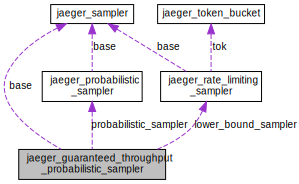
\includegraphics[width=350pt]{structjaeger__guaranteed__throughput__probabilistic__sampler__coll__graph}
\end{center}
\end{figure}
\subsection*{Data Fields}
\begin{DoxyCompactItemize}
\item 
\mbox{\Hypertarget{structjaeger__guaranteed__throughput__probabilistic__sampler_a82d1383e728fd205b2b13c63314f2e43}\label{structjaeger__guaranteed__throughput__probabilistic__sampler_a82d1383e728fd205b2b13c63314f2e43}} 
\mbox{\hyperlink{structjaeger__sampler}{jaeger\+\_\+sampler}} {\bfseries base}
\item 
\mbox{\Hypertarget{structjaeger__guaranteed__throughput__probabilistic__sampler_afa54809aa0b0c6a4a5aad2e4314bd766}\label{structjaeger__guaranteed__throughput__probabilistic__sampler_afa54809aa0b0c6a4a5aad2e4314bd766}} 
\mbox{\hyperlink{structjaeger__probabilistic__sampler}{jaeger\+\_\+probabilistic\+\_\+sampler}} {\bfseries probabilistic\+\_\+sampler}
\item 
\mbox{\Hypertarget{structjaeger__guaranteed__throughput__probabilistic__sampler_a80af8b3ac612320c6a00e4655e25f694}\label{structjaeger__guaranteed__throughput__probabilistic__sampler_a80af8b3ac612320c6a00e4655e25f694}} 
\mbox{\hyperlink{structjaeger__rate__limiting__sampler}{jaeger\+\_\+rate\+\_\+limiting\+\_\+sampler}} {\bfseries lower\+\_\+bound\+\_\+sampler}
\end{DoxyCompactItemize}


The documentation for this struct was generated from the following file\+:\begin{DoxyCompactItemize}
\item 
jaegertracingc/\mbox{\hyperlink{sampler_8h}{sampler.\+h}}\end{DoxyCompactItemize}

\hypertarget{structjaeger__hashtable}{}\section{jaeger\+\_\+hashtable Struct Reference}
\label{structjaeger__hashtable}\index{jaeger\+\_\+hashtable@{jaeger\+\_\+hashtable}}


Hashtable data structure.  




{\ttfamily \#include $<$jaegertracingc/hashtable.\+h$>$}



Collaboration diagram for jaeger\+\_\+hashtable\+:\nopagebreak
\begin{figure}[H]
\begin{center}
\leavevmode
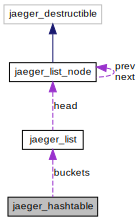
\includegraphics[width=213pt]{structjaeger__hashtable__coll__graph}
\end{center}
\end{figure}
\subsection*{Data Fields}
\begin{DoxyCompactItemize}
\item 
\mbox{\Hypertarget{structjaeger__hashtable_a7afd4995727f79226cfb90d75b3db555}\label{structjaeger__hashtable_a7afd4995727f79226cfb90d75b3db555}} 
size\+\_\+t {\bfseries size}
\item 
\mbox{\Hypertarget{structjaeger__hashtable_a6c640cb2545575f3dc97ccecad8fa2e2}\label{structjaeger__hashtable_a6c640cb2545575f3dc97ccecad8fa2e2}} 
size\+\_\+t {\bfseries order}
\item 
\mbox{\Hypertarget{structjaeger__hashtable_af283e63203deff3a9793c3817244e59c}\label{structjaeger__hashtable_af283e63203deff3a9793c3817244e59c}} 
\mbox{\hyperlink{structjaeger__list}{jaeger\+\_\+list}} $\ast$ {\bfseries buckets}
\end{DoxyCompactItemize}


\subsection{Detailed Description}
Hashtable data structure. 

The documentation for this struct was generated from the following file\+:\begin{DoxyCompactItemize}
\item 
jaegertracingc/\mbox{\hyperlink{hashtable_8h}{hashtable.\+h}}\end{DoxyCompactItemize}

\hypertarget{structjaeger__hashtable__lookup__result}{}\section{jaeger\+\_\+hashtable\+\_\+lookup\+\_\+result Struct Reference}
\label{structjaeger__hashtable__lookup__result}\index{jaeger\+\_\+hashtable\+\_\+lookup\+\_\+result@{jaeger\+\_\+hashtable\+\_\+lookup\+\_\+result}}


Collaboration diagram for jaeger\+\_\+hashtable\+\_\+lookup\+\_\+result\+:\nopagebreak
\begin{figure}[H]
\begin{center}
\leavevmode
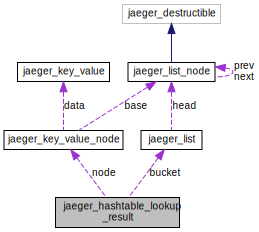
\includegraphics[width=331pt]{structjaeger__hashtable__lookup__result__coll__graph}
\end{center}
\end{figure}
\subsection*{Data Fields}
\begin{DoxyCompactItemize}
\item 
\mbox{\Hypertarget{structjaeger__hashtable__lookup__result_a840c3a7e03d125c18851a69f4334c989}\label{structjaeger__hashtable__lookup__result_a840c3a7e03d125c18851a69f4334c989}} 
\mbox{\hyperlink{structjaeger__key__value__node}{jaeger\+\_\+key\+\_\+value\+\_\+node}} $\ast$ {\bfseries node}
\item 
\mbox{\Hypertarget{structjaeger__hashtable__lookup__result_a445935b25b84db16ba06be06638625ee}\label{structjaeger__hashtable__lookup__result_a445935b25b84db16ba06be06638625ee}} 
\mbox{\hyperlink{structjaeger__list}{jaeger\+\_\+list}} $\ast$ {\bfseries bucket}
\end{DoxyCompactItemize}


The documentation for this struct was generated from the following file\+:\begin{DoxyCompactItemize}
\item 
jaegertracingc/\mbox{\hyperlink{hashtable_8h}{hashtable.\+h}}\end{DoxyCompactItemize}

\hypertarget{structjaeger__headers__config}{}\section{jaeger\+\_\+headers\+\_\+config Struct Reference}
\label{structjaeger__headers__config}\index{jaeger\+\_\+headers\+\_\+config@{jaeger\+\_\+headers\+\_\+config}}


H\+T\+TP headers to use for span context propagation.  




{\ttfamily \#include $<$jaegertracingc/options.\+h$>$}

\subsection*{Data Fields}
\begin{DoxyCompactItemize}
\item 
const char $\ast$ \mbox{\hyperlink{structjaeger__headers__config_aab0510e85c8d184cdd7e1afd41f344c3}{debug\+\_\+header}}
\begin{DoxyCompactList}\small\item\em Header used to propagate a debug span. \end{DoxyCompactList}\item 
const char $\ast$ \mbox{\hyperlink{structjaeger__headers__config_ae803931b2f758163162a55b511021a1c}{baggage\+\_\+header}}
\begin{DoxyCompactList}\small\item\em Header used to propagate baggage. \end{DoxyCompactList}\item 
const char $\ast$ \mbox{\hyperlink{structjaeger__headers__config_a5aee0f70ee5455509ee2839636369a83}{trace\+\_\+context\+\_\+header}}
\begin{DoxyCompactList}\small\item\em Header used to propagate a span context. \end{DoxyCompactList}\item 
const char $\ast$ \mbox{\hyperlink{structjaeger__headers__config_aaa9702c861bf4f0c346f65bb54de0110}{trace\+\_\+baggage\+\_\+header\+\_\+prefix}}
\begin{DoxyCompactList}\small\item\em Header prefix to prepend to baggage keys. \end{DoxyCompactList}\end{DoxyCompactItemize}


\subsection{Detailed Description}
H\+T\+TP headers to use for span context propagation. 

\subsection{Field Documentation}
\mbox{\Hypertarget{structjaeger__headers__config_ae803931b2f758163162a55b511021a1c}\label{structjaeger__headers__config_ae803931b2f758163162a55b511021a1c}} 
\index{jaeger\+\_\+headers\+\_\+config@{jaeger\+\_\+headers\+\_\+config}!baggage\+\_\+header@{baggage\+\_\+header}}
\index{baggage\+\_\+header@{baggage\+\_\+header}!jaeger\+\_\+headers\+\_\+config@{jaeger\+\_\+headers\+\_\+config}}
\subsubsection{\texorpdfstring{baggage\+\_\+header}{baggage\_header}}
{\footnotesize\ttfamily const char$\ast$ jaeger\+\_\+headers\+\_\+config\+::baggage\+\_\+header}



Header used to propagate baggage. 

\mbox{\Hypertarget{structjaeger__headers__config_aab0510e85c8d184cdd7e1afd41f344c3}\label{structjaeger__headers__config_aab0510e85c8d184cdd7e1afd41f344c3}} 
\index{jaeger\+\_\+headers\+\_\+config@{jaeger\+\_\+headers\+\_\+config}!debug\+\_\+header@{debug\+\_\+header}}
\index{debug\+\_\+header@{debug\+\_\+header}!jaeger\+\_\+headers\+\_\+config@{jaeger\+\_\+headers\+\_\+config}}
\subsubsection{\texorpdfstring{debug\+\_\+header}{debug\_header}}
{\footnotesize\ttfamily const char$\ast$ jaeger\+\_\+headers\+\_\+config\+::debug\+\_\+header}



Header used to propagate a debug span. 

\mbox{\Hypertarget{structjaeger__headers__config_aaa9702c861bf4f0c346f65bb54de0110}\label{structjaeger__headers__config_aaa9702c861bf4f0c346f65bb54de0110}} 
\index{jaeger\+\_\+headers\+\_\+config@{jaeger\+\_\+headers\+\_\+config}!trace\+\_\+baggage\+\_\+header\+\_\+prefix@{trace\+\_\+baggage\+\_\+header\+\_\+prefix}}
\index{trace\+\_\+baggage\+\_\+header\+\_\+prefix@{trace\+\_\+baggage\+\_\+header\+\_\+prefix}!jaeger\+\_\+headers\+\_\+config@{jaeger\+\_\+headers\+\_\+config}}
\subsubsection{\texorpdfstring{trace\+\_\+baggage\+\_\+header\+\_\+prefix}{trace\_baggage\_header\_prefix}}
{\footnotesize\ttfamily const char$\ast$ jaeger\+\_\+headers\+\_\+config\+::trace\+\_\+baggage\+\_\+header\+\_\+prefix}



Header prefix to prepend to baggage keys. 

\mbox{\Hypertarget{structjaeger__headers__config_a5aee0f70ee5455509ee2839636369a83}\label{structjaeger__headers__config_a5aee0f70ee5455509ee2839636369a83}} 
\index{jaeger\+\_\+headers\+\_\+config@{jaeger\+\_\+headers\+\_\+config}!trace\+\_\+context\+\_\+header@{trace\+\_\+context\+\_\+header}}
\index{trace\+\_\+context\+\_\+header@{trace\+\_\+context\+\_\+header}!jaeger\+\_\+headers\+\_\+config@{jaeger\+\_\+headers\+\_\+config}}
\subsubsection{\texorpdfstring{trace\+\_\+context\+\_\+header}{trace\_context\_header}}
{\footnotesize\ttfamily const char$\ast$ jaeger\+\_\+headers\+\_\+config\+::trace\+\_\+context\+\_\+header}



Header used to propagate a span context. 



The documentation for this struct was generated from the following file\+:\begin{DoxyCompactItemize}
\item 
jaegertracingc/\mbox{\hyperlink{options_8h}{options.\+h}}\end{DoxyCompactItemize}

\hypertarget{structjaeger__host__port}{}\section{jaeger\+\_\+host\+\_\+port Struct Reference}
\label{structjaeger__host__port}\index{jaeger\+\_\+host\+\_\+port@{jaeger\+\_\+host\+\_\+port}}
\subsection*{Data Fields}
\begin{DoxyCompactItemize}
\item 
\mbox{\Hypertarget{structjaeger__host__port_af0dd78d71f61efd2834cbe2ade69aae2}\label{structjaeger__host__port_af0dd78d71f61efd2834cbe2ade69aae2}} 
char $\ast$ {\bfseries host}
\item 
\mbox{\Hypertarget{structjaeger__host__port_a1b326a3a83c046429052e71560a16c8e}\label{structjaeger__host__port_a1b326a3a83c046429052e71560a16c8e}} 
int {\bfseries port}
\end{DoxyCompactItemize}


The documentation for this struct was generated from the following file\+:\begin{DoxyCompactItemize}
\item 
jaegertracingc/\mbox{\hyperlink{net_8h}{net.\+h}}\end{DoxyCompactItemize}

\hypertarget{structjaeger__http__sampling__manager}{}\section{jaeger\+\_\+http\+\_\+sampling\+\_\+manager Struct Reference}
\label{structjaeger__http__sampling__manager}\index{jaeger\+\_\+http\+\_\+sampling\+\_\+manager@{jaeger\+\_\+http\+\_\+sampling\+\_\+manager}}


Collaboration diagram for jaeger\+\_\+http\+\_\+sampling\+\_\+manager\+:\nopagebreak
\begin{figure}[H]
\begin{center}
\leavevmode
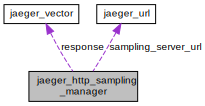
\includegraphics[width=278pt]{structjaeger__http__sampling__manager__coll__graph}
\end{center}
\end{figure}
\subsection*{Data Fields}
\begin{DoxyCompactItemize}
\item 
\mbox{\Hypertarget{structjaeger__http__sampling__manager_a3d951ac4fa00733acbbf594e46eed2ca}\label{structjaeger__http__sampling__manager_a3d951ac4fa00733acbbf594e46eed2ca}} 
char $\ast$ {\bfseries service\+\_\+name}
\item 
\mbox{\Hypertarget{structjaeger__http__sampling__manager_a5c107ffae64e23dfc4e6d5d89ae8920e}\label{structjaeger__http__sampling__manager_a5c107ffae64e23dfc4e6d5d89ae8920e}} 
\mbox{\hyperlink{structjaeger__url}{jaeger\+\_\+url}} {\bfseries sampling\+\_\+server\+\_\+url}
\item 
\mbox{\Hypertarget{structjaeger__http__sampling__manager_a5831094db16cbb7f08ee0733ce5861cf}\label{structjaeger__http__sampling__manager_a5831094db16cbb7f08ee0733ce5861cf}} 
int {\bfseries fd}
\item 
\mbox{\Hypertarget{structjaeger__http__sampling__manager_a0393fb1be95b7a6f9c42bd426855c96b}\label{structjaeger__http__sampling__manager_a0393fb1be95b7a6f9c42bd426855c96b}} 
http\+\_\+parser {\bfseries parser}
\item 
\mbox{\Hypertarget{structjaeger__http__sampling__manager_aba8b8b9ad94bb73a1a613de8e6cbf9cd}\label{structjaeger__http__sampling__manager_aba8b8b9ad94bb73a1a613de8e6cbf9cd}} 
http\+\_\+parser\+\_\+settings {\bfseries settings}
\item 
\mbox{\Hypertarget{structjaeger__http__sampling__manager_a199ab3b2a3f1e32295093771dfafa634}\label{structjaeger__http__sampling__manager_a199ab3b2a3f1e32295093771dfafa634}} 
int {\bfseries request\+\_\+length}
\item 
\mbox{\Hypertarget{structjaeger__http__sampling__manager_a342eb6eab82e1383e540f246642c2872}\label{structjaeger__http__sampling__manager_a342eb6eab82e1383e540f246642c2872}} 
char {\bfseries request\+\_\+buffer} \mbox{[}256\mbox{]}
\item 
\mbox{\Hypertarget{structjaeger__http__sampling__manager_a561df2066ae877b36bfd21e5caab2e38}\label{structjaeger__http__sampling__manager_a561df2066ae877b36bfd21e5caab2e38}} 
\mbox{\hyperlink{structjaeger__vector}{jaeger\+\_\+vector}} {\bfseries response}
\end{DoxyCompactItemize}


The documentation for this struct was generated from the following file\+:\begin{DoxyCompactItemize}
\item 
jaegertracingc/\mbox{\hyperlink{sampler_8h}{sampler.\+h}}\end{DoxyCompactItemize}

\hypertarget{structjaeger__in__memory__reporter}{}\section{jaeger\+\_\+in\+\_\+memory\+\_\+reporter Struct Reference}
\label{structjaeger__in__memory__reporter}\index{jaeger\+\_\+in\+\_\+memory\+\_\+reporter@{jaeger\+\_\+in\+\_\+memory\+\_\+reporter}}


Collaboration diagram for jaeger\+\_\+in\+\_\+memory\+\_\+reporter\+:\nopagebreak
\begin{figure}[H]
\begin{center}
\leavevmode
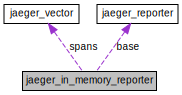
\includegraphics[width=254pt]{structjaeger__in__memory__reporter__coll__graph}
\end{center}
\end{figure}
\subsection*{Data Fields}
\begin{DoxyCompactItemize}
\item 
\mbox{\Hypertarget{structjaeger__in__memory__reporter_a420c17c75738dfa9bf542aa2ead56ffb}\label{structjaeger__in__memory__reporter_a420c17c75738dfa9bf542aa2ead56ffb}} 
\mbox{\hyperlink{structjaeger__reporter}{jaeger\+\_\+reporter}} {\bfseries base}
\item 
\mbox{\Hypertarget{structjaeger__in__memory__reporter_a97011975d7f93b051764da153deab7d0}\label{structjaeger__in__memory__reporter_a97011975d7f93b051764da153deab7d0}} 
\mbox{\hyperlink{structjaeger__vector}{jaeger\+\_\+vector}} {\bfseries spans}
\item 
\mbox{\Hypertarget{structjaeger__in__memory__reporter_abf881ed3f4f1f4dba522de60831b8bf9}\label{structjaeger__in__memory__reporter_abf881ed3f4f1f4dba522de60831b8bf9}} 
jaeger\+\_\+mutex {\bfseries mutex}
\end{DoxyCompactItemize}


The documentation for this struct was generated from the following file\+:\begin{DoxyCompactItemize}
\item 
jaegertracingc/\mbox{\hyperlink{reporter_8h}{reporter.\+h}}\end{DoxyCompactItemize}

\hypertarget{structjaeger__key__value}{}\section{jaeger\+\_\+key\+\_\+value Struct Reference}
\label{structjaeger__key__value}\index{jaeger\+\_\+key\+\_\+value@{jaeger\+\_\+key\+\_\+value}}
\subsection*{Data Fields}
\begin{DoxyCompactItemize}
\item 
\mbox{\Hypertarget{structjaeger__key__value_a0c8d3423ffabd9b686aa0c7abd6889d4}\label{structjaeger__key__value_a0c8d3423ffabd9b686aa0c7abd6889d4}} 
char $\ast$ {\bfseries key}
\item 
\mbox{\Hypertarget{structjaeger__key__value_ab79cc266eb0080ecb608b57896ad4037}\label{structjaeger__key__value_ab79cc266eb0080ecb608b57896ad4037}} 
char $\ast$ {\bfseries value}
\end{DoxyCompactItemize}


The documentation for this struct was generated from the following file\+:\begin{DoxyCompactItemize}
\item 
jaegertracingc/\mbox{\hyperlink{key__value_8h}{key\+\_\+value.\+h}}\end{DoxyCompactItemize}

\hypertarget{structjaeger__key__value__node}{}\section{jaeger\+\_\+key\+\_\+value\+\_\+node Struct Reference}
\label{structjaeger__key__value__node}\index{jaeger\+\_\+key\+\_\+value\+\_\+node@{jaeger\+\_\+key\+\_\+value\+\_\+node}}


Define link list node for key-\/value pairs.  




{\ttfamily \#include $<$jaegertracingc/hashtable.\+h$>$}



Collaboration diagram for jaeger\+\_\+key\+\_\+value\+\_\+node\+:\nopagebreak
\begin{figure}[H]
\begin{center}
\leavevmode
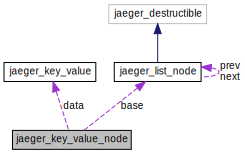
\includegraphics[width=318pt]{structjaeger__key__value__node__coll__graph}
\end{center}
\end{figure}
\subsection*{Data Fields}
\begin{DoxyCompactItemize}
\item 
\mbox{\Hypertarget{structjaeger__key__value__node_a590784cfceafeb3ec9ec12c9b67e6867}\label{structjaeger__key__value__node_a590784cfceafeb3ec9ec12c9b67e6867}} 
\mbox{\hyperlink{structjaeger__list__node}{jaeger\+\_\+list\+\_\+node}} {\bfseries base}
\item 
\mbox{\Hypertarget{structjaeger__key__value__node_a28ce993b369e2e969d524d7c65db2f9f}\label{structjaeger__key__value__node_a28ce993b369e2e969d524d7c65db2f9f}} 
\mbox{\hyperlink{structjaeger__key__value}{jaeger\+\_\+key\+\_\+value}} {\bfseries data}
\end{DoxyCompactItemize}


\subsection{Detailed Description}
Define link list node for key-\/value pairs. 



The documentation for this struct was generated from the following file\+:\begin{DoxyCompactItemize}
\item 
jaegertracingc/\mbox{\hyperlink{hashtable_8h}{hashtable.\+h}}\end{DoxyCompactItemize}

\hypertarget{structjaeger__list}{}\section{jaeger\+\_\+list Struct Reference}
\label{structjaeger__list}\index{jaeger\+\_\+list@{jaeger\+\_\+list}}


Linked list implementation.  




{\ttfamily \#include $<$jaegertracingc/list.\+h$>$}



Collaboration diagram for jaeger\+\_\+list\+:\nopagebreak
\begin{figure}[H]
\begin{center}
\leavevmode
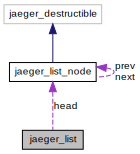
\includegraphics[width=213pt]{structjaeger__list__coll__graph}
\end{center}
\end{figure}
\subsection*{Data Fields}
\begin{DoxyCompactItemize}
\item 
\mbox{\hyperlink{structjaeger__list__node}{jaeger\+\_\+list\+\_\+node}} $\ast$ \mbox{\hyperlink{structjaeger__list_ad5a459e896a2bd718d633c63fecf695a}{head}}
\begin{DoxyCompactList}\small\item\em Head of list. \end{DoxyCompactList}\item 
size\+\_\+t \mbox{\hyperlink{structjaeger__list_a8bb149f40b7a39dcaf99481570f91afc}{size}}
\begin{DoxyCompactList}\small\item\em Size of list. \end{DoxyCompactList}\end{DoxyCompactItemize}


\subsection{Detailed Description}
Linked list implementation. 



\subsection{Field Documentation}
\mbox{\Hypertarget{structjaeger__list_ad5a459e896a2bd718d633c63fecf695a}\label{structjaeger__list_ad5a459e896a2bd718d633c63fecf695a}} 
\index{jaeger\+\_\+list@{jaeger\+\_\+list}!head@{head}}
\index{head@{head}!jaeger\+\_\+list@{jaeger\+\_\+list}}
\subsubsection{\texorpdfstring{head}{head}}
{\footnotesize\ttfamily \mbox{\hyperlink{structjaeger__list__node}{jaeger\+\_\+list\+\_\+node}}$\ast$ jaeger\+\_\+list\+::head}



Head of list. 

\mbox{\Hypertarget{structjaeger__list_a8bb149f40b7a39dcaf99481570f91afc}\label{structjaeger__list_a8bb149f40b7a39dcaf99481570f91afc}} 
\index{jaeger\+\_\+list@{jaeger\+\_\+list}!size@{size}}
\index{size@{size}!jaeger\+\_\+list@{jaeger\+\_\+list}}
\subsubsection{\texorpdfstring{size}{size}}
{\footnotesize\ttfamily size\+\_\+t jaeger\+\_\+list\+::size}



Size of list. 

Avoids counting via traversing. 

The documentation for this struct was generated from the following file\+:\begin{DoxyCompactItemize}
\item 
jaegertracingc/list.\+h\end{DoxyCompactItemize}

\hypertarget{structjaeger__list__node}{}\section{jaeger\+\_\+list\+\_\+node Struct Reference}
\label{structjaeger__list__node}\index{jaeger\+\_\+list\+\_\+node@{jaeger\+\_\+list\+\_\+node}}


Base class for list elements.  




{\ttfamily \#include $<$jaegertracingc/list.\+h$>$}



Inheritance diagram for jaeger\+\_\+list\+\_\+node\+:\nopagebreak
\begin{figure}[H]
\begin{center}
\leavevmode
\includegraphics[width=178pt]{structjaeger__list__node__inherit__graph}
\end{center}
\end{figure}


Collaboration diagram for jaeger\+\_\+list\+\_\+node\+:\nopagebreak
\begin{figure}[H]
\begin{center}
\leavevmode
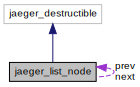
\includegraphics[width=213pt]{structjaeger__list__node__coll__graph}
\end{center}
\end{figure}
\subsection*{Data Fields}
\begin{DoxyCompactItemize}
\item 
jaeger\+\_\+destructible \mbox{\hyperlink{structjaeger__list__node_aff2082a8eaa51bcb60f131401d37a549}{base}}
\begin{DoxyCompactList}\small\item\em Base class member. \end{DoxyCompactList}\item 
struct \mbox{\hyperlink{structjaeger__list__node}{jaeger\+\_\+list\+\_\+node}} $\ast$ \mbox{\hyperlink{structjaeger__list__node_a2bb6e6f98c5f2e335ed4e97c2175c78f}{prev}}
\begin{DoxyCompactList}\small\item\em Pointer to previous node. \end{DoxyCompactList}\item 
struct \mbox{\hyperlink{structjaeger__list__node}{jaeger\+\_\+list\+\_\+node}} $\ast$ \mbox{\hyperlink{structjaeger__list__node_a06dd6747b4a3001ea24a0aa33741d126}{next}}
\begin{DoxyCompactList}\small\item\em Pointer to next node. \end{DoxyCompactList}\end{DoxyCompactItemize}


\subsection{Detailed Description}
Base class for list elements. 

\subsection{Field Documentation}
\mbox{\Hypertarget{structjaeger__list__node_aff2082a8eaa51bcb60f131401d37a549}\label{structjaeger__list__node_aff2082a8eaa51bcb60f131401d37a549}} 
\index{jaeger\+\_\+list\+\_\+node@{jaeger\+\_\+list\+\_\+node}!base@{base}}
\index{base@{base}!jaeger\+\_\+list\+\_\+node@{jaeger\+\_\+list\+\_\+node}}
\subsubsection{\texorpdfstring{base}{base}}
{\footnotesize\ttfamily jaeger\+\_\+destructible jaeger\+\_\+list\+\_\+node\+::base}



Base class member. 

\mbox{\Hypertarget{structjaeger__list__node_a06dd6747b4a3001ea24a0aa33741d126}\label{structjaeger__list__node_a06dd6747b4a3001ea24a0aa33741d126}} 
\index{jaeger\+\_\+list\+\_\+node@{jaeger\+\_\+list\+\_\+node}!next@{next}}
\index{next@{next}!jaeger\+\_\+list\+\_\+node@{jaeger\+\_\+list\+\_\+node}}
\subsubsection{\texorpdfstring{next}{next}}
{\footnotesize\ttfamily struct \mbox{\hyperlink{structjaeger__list__node}{jaeger\+\_\+list\+\_\+node}}$\ast$ jaeger\+\_\+list\+\_\+node\+::next}



Pointer to next node. 

\mbox{\Hypertarget{structjaeger__list__node_a2bb6e6f98c5f2e335ed4e97c2175c78f}\label{structjaeger__list__node_a2bb6e6f98c5f2e335ed4e97c2175c78f}} 
\index{jaeger\+\_\+list\+\_\+node@{jaeger\+\_\+list\+\_\+node}!prev@{prev}}
\index{prev@{prev}!jaeger\+\_\+list\+\_\+node@{jaeger\+\_\+list\+\_\+node}}
\subsubsection{\texorpdfstring{prev}{prev}}
{\footnotesize\ttfamily struct \mbox{\hyperlink{structjaeger__list__node}{jaeger\+\_\+list\+\_\+node}}$\ast$ jaeger\+\_\+list\+\_\+node\+::prev}



Pointer to previous node. 



The documentation for this struct was generated from the following file\+:\begin{DoxyCompactItemize}
\item 
jaegertracingc/list.\+h\end{DoxyCompactItemize}

\hypertarget{structjaeger__log__record}{}\section{jaeger\+\_\+log\+\_\+record Struct Reference}
\label{structjaeger__log__record}\index{jaeger\+\_\+log\+\_\+record@{jaeger\+\_\+log\+\_\+record}}


Collaboration diagram for jaeger\+\_\+log\+\_\+record\+:\nopagebreak
\begin{figure}[H]
\begin{center}
\leavevmode
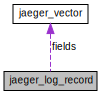
\includegraphics[width=173pt]{structjaeger__log__record__coll__graph}
\end{center}
\end{figure}
\subsection*{Data Fields}
\begin{DoxyCompactItemize}
\item 
\mbox{\Hypertarget{structjaeger__log__record_a0ccac56ec47a1f065b0a38b17d0c7a07}\label{structjaeger__log__record_a0ccac56ec47a1f065b0a38b17d0c7a07}} 
jaeger\+\_\+timestamp {\bfseries timestamp}
\item 
\mbox{\Hypertarget{structjaeger__log__record_a7e92d49bbf95a25adf10d22d0c87c70f}\label{structjaeger__log__record_a7e92d49bbf95a25adf10d22d0c87c70f}} 
\mbox{\hyperlink{structjaeger__vector}{jaeger\+\_\+vector}} {\bfseries fields}
\end{DoxyCompactItemize}


The documentation for this struct was generated from the following file\+:\begin{DoxyCompactItemize}
\item 
jaegertracingc/\mbox{\hyperlink{log__record_8h}{log\+\_\+record.\+h}}\end{DoxyCompactItemize}

\hypertarget{structjaeger__logger}{}\section{jaeger\+\_\+logger Struct Reference}
\label{structjaeger__logger}\index{jaeger\+\_\+logger@{jaeger\+\_\+logger}}


Logger interface to customize log output.  




{\ttfamily \#include $<$jaegertracingc/logging.\+h$>$}

\subsection*{Data Fields}
\begin{DoxyCompactItemize}
\item 
void($\ast$ \mbox{\hyperlink{structjaeger__logger_a41a2e4729ee8379193fe61dd5113bda6}{error}} )(struct \mbox{\hyperlink{structjaeger__logger}{jaeger\+\_\+logger}} $\ast$logger, const char $\ast$format, va\+\_\+list args)
\begin{DoxyCompactList}\small\item\em Error log function. \end{DoxyCompactList}\item 
void($\ast$ \mbox{\hyperlink{structjaeger__logger_a92ed10ab8a9826819eca22027258ae16}{warn}} )(struct \mbox{\hyperlink{structjaeger__logger}{jaeger\+\_\+logger}} $\ast$logger, const char $\ast$format, va\+\_\+list args)
\begin{DoxyCompactList}\small\item\em Warn log function. \end{DoxyCompactList}\item 
void($\ast$ \mbox{\hyperlink{structjaeger__logger_af6b893184914a085c831e26f10c2b4c6}{info}} )(struct \mbox{\hyperlink{structjaeger__logger}{jaeger\+\_\+logger}} $\ast$logger, const char $\ast$format, va\+\_\+list args)
\begin{DoxyCompactList}\small\item\em Info log function. \end{DoxyCompactList}\end{DoxyCompactItemize}


\subsection{Detailed Description}
Logger interface to customize log output. 



\subsection{Field Documentation}
\mbox{\Hypertarget{structjaeger__logger_a41a2e4729ee8379193fe61dd5113bda6}\label{structjaeger__logger_a41a2e4729ee8379193fe61dd5113bda6}} 
\index{jaeger\+\_\+logger@{jaeger\+\_\+logger}!error@{error}}
\index{error@{error}!jaeger\+\_\+logger@{jaeger\+\_\+logger}}
\subsubsection{\texorpdfstring{error}{error}}
{\footnotesize\ttfamily void($\ast$ jaeger\+\_\+logger\+::error) (struct \mbox{\hyperlink{structjaeger__logger}{jaeger\+\_\+logger}} $\ast$logger, const char $\ast$format, va\+\_\+list args)}



Error log function. 


\begin{DoxyParams}[1]{Parameters}
 & {\em logger} & Logger instance. \\
\hline
 & {\em format} & Format string of the message. \\
\hline
\mbox{\tt in}  & {\em ...} & Arguments to format. \\
\hline
\end{DoxyParams}
\mbox{\Hypertarget{structjaeger__logger_af6b893184914a085c831e26f10c2b4c6}\label{structjaeger__logger_af6b893184914a085c831e26f10c2b4c6}} 
\index{jaeger\+\_\+logger@{jaeger\+\_\+logger}!info@{info}}
\index{info@{info}!jaeger\+\_\+logger@{jaeger\+\_\+logger}}
\subsubsection{\texorpdfstring{info}{info}}
{\footnotesize\ttfamily void($\ast$ jaeger\+\_\+logger\+::info) (struct \mbox{\hyperlink{structjaeger__logger}{jaeger\+\_\+logger}} $\ast$logger, const char $\ast$format, va\+\_\+list args)}



Info log function. 


\begin{DoxyParams}[1]{Parameters}
 & {\em logger} & Logger instance. \\
\hline
 & {\em format} & Format string of the message. \\
\hline
\mbox{\tt in}  & {\em ...} & Arguments to format. \\
\hline
\end{DoxyParams}
\mbox{\Hypertarget{structjaeger__logger_a92ed10ab8a9826819eca22027258ae16}\label{structjaeger__logger_a92ed10ab8a9826819eca22027258ae16}} 
\index{jaeger\+\_\+logger@{jaeger\+\_\+logger}!warn@{warn}}
\index{warn@{warn}!jaeger\+\_\+logger@{jaeger\+\_\+logger}}
\subsubsection{\texorpdfstring{warn}{warn}}
{\footnotesize\ttfamily void($\ast$ jaeger\+\_\+logger\+::warn) (struct \mbox{\hyperlink{structjaeger__logger}{jaeger\+\_\+logger}} $\ast$logger, const char $\ast$format, va\+\_\+list args)}



Warn log function. 


\begin{DoxyParams}[1]{Parameters}
 & {\em logger} & Logger instance. \\
\hline
 & {\em format} & Format string of the message. \\
\hline
\mbox{\tt in}  & {\em ...} & Arguments to format. \\
\hline
\end{DoxyParams}


The documentation for this struct was generated from the following file\+:\begin{DoxyCompactItemize}
\item 
jaegertracingc/\mbox{\hyperlink{logging_8h}{logging.\+h}}\end{DoxyCompactItemize}

\hypertarget{structjaeger__metrics}{}\section{jaeger\+\_\+metrics Struct Reference}
\label{structjaeger__metrics}\index{jaeger\+\_\+metrics@{jaeger\+\_\+metrics}}


Collaboration diagram for jaeger\+\_\+metrics\+:\nopagebreak
\begin{figure}[H]
\begin{center}
\leavevmode
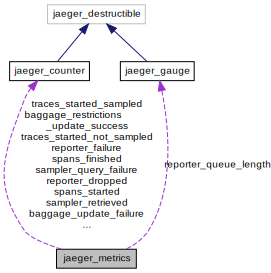
\includegraphics[width=344pt]{structjaeger__metrics__coll__graph}
\end{center}
\end{figure}
\subsection*{Data Fields}
\begin{DoxyCompactItemize}
\item 
\mbox{\Hypertarget{structjaeger__metrics_a6aec22e6be01c7926b9c97a9abe6b48f}\label{structjaeger__metrics_a6aec22e6be01c7926b9c97a9abe6b48f}} 
\mbox{\hyperlink{structjaeger__counter}{jaeger\+\_\+counter}} $\ast$ {\bfseries traces\+\_\+started\+\_\+sampled}
\item 
\mbox{\Hypertarget{structjaeger__metrics_afec1c6ec9640195dc84142740ab7e50c}\label{structjaeger__metrics_afec1c6ec9640195dc84142740ab7e50c}} 
\mbox{\hyperlink{structjaeger__counter}{jaeger\+\_\+counter}} $\ast$ {\bfseries traces\+\_\+started\+\_\+not\+\_\+sampled}
\item 
\mbox{\Hypertarget{structjaeger__metrics_a5662180018d2ad04cb5b8b5dc837d3f2}\label{structjaeger__metrics_a5662180018d2ad04cb5b8b5dc837d3f2}} 
\mbox{\hyperlink{structjaeger__counter}{jaeger\+\_\+counter}} $\ast$ {\bfseries traces\+\_\+joined\+\_\+sampled}
\item 
\mbox{\Hypertarget{structjaeger__metrics_a27d29942ffffda19a4837446eb66ab71}\label{structjaeger__metrics_a27d29942ffffda19a4837446eb66ab71}} 
\mbox{\hyperlink{structjaeger__counter}{jaeger\+\_\+counter}} $\ast$ {\bfseries traces\+\_\+joined\+\_\+not\+\_\+sampled}
\item 
\mbox{\Hypertarget{structjaeger__metrics_a7bdd0ea8c240c8b0891c36bb0372525b}\label{structjaeger__metrics_a7bdd0ea8c240c8b0891c36bb0372525b}} 
\mbox{\hyperlink{structjaeger__counter}{jaeger\+\_\+counter}} $\ast$ {\bfseries spans\+\_\+started}
\item 
\mbox{\Hypertarget{structjaeger__metrics_ae1d08e8f7978b3007bd918e089aafb1e}\label{structjaeger__metrics_ae1d08e8f7978b3007bd918e089aafb1e}} 
\mbox{\hyperlink{structjaeger__counter}{jaeger\+\_\+counter}} $\ast$ {\bfseries spans\+\_\+finished}
\item 
\mbox{\Hypertarget{structjaeger__metrics_a717a3241ce74f1de6a978e4ecad2454c}\label{structjaeger__metrics_a717a3241ce74f1de6a978e4ecad2454c}} 
\mbox{\hyperlink{structjaeger__counter}{jaeger\+\_\+counter}} $\ast$ {\bfseries spans\+\_\+sampled}
\item 
\mbox{\Hypertarget{structjaeger__metrics_a3ddaffc27eef9908996e3fc3012f252c}\label{structjaeger__metrics_a3ddaffc27eef9908996e3fc3012f252c}} 
\mbox{\hyperlink{structjaeger__counter}{jaeger\+\_\+counter}} $\ast$ {\bfseries spans\+\_\+not\+\_\+sampled}
\item 
\mbox{\Hypertarget{structjaeger__metrics_a195d345d105050793bde0f54bb324065}\label{structjaeger__metrics_a195d345d105050793bde0f54bb324065}} 
\mbox{\hyperlink{structjaeger__counter}{jaeger\+\_\+counter}} $\ast$ {\bfseries decoding\+\_\+errors}
\item 
\mbox{\Hypertarget{structjaeger__metrics_a126218eb9288429de226499c665335ed}\label{structjaeger__metrics_a126218eb9288429de226499c665335ed}} 
\mbox{\hyperlink{structjaeger__counter}{jaeger\+\_\+counter}} $\ast$ {\bfseries reporter\+\_\+success}
\item 
\mbox{\Hypertarget{structjaeger__metrics_a6e083d07098a4d4ea88f6104d489da93}\label{structjaeger__metrics_a6e083d07098a4d4ea88f6104d489da93}} 
\mbox{\hyperlink{structjaeger__counter}{jaeger\+\_\+counter}} $\ast$ {\bfseries reporter\+\_\+failure}
\item 
\mbox{\Hypertarget{structjaeger__metrics_a96f65c9e581b1ec471ab6ba7be4166f5}\label{structjaeger__metrics_a96f65c9e581b1ec471ab6ba7be4166f5}} 
\mbox{\hyperlink{structjaeger__counter}{jaeger\+\_\+counter}} $\ast$ {\bfseries reporter\+\_\+dropped}
\item 
\mbox{\Hypertarget{structjaeger__metrics_a55c15e5e17671e5189f283be515398fc}\label{structjaeger__metrics_a55c15e5e17671e5189f283be515398fc}} 
\mbox{\hyperlink{structjaeger__counter}{jaeger\+\_\+counter}} $\ast$ {\bfseries sampler\+\_\+retrieved}
\item 
\mbox{\Hypertarget{structjaeger__metrics_a41d77edff148e36ed6346d18c72222dc}\label{structjaeger__metrics_a41d77edff148e36ed6346d18c72222dc}} 
\mbox{\hyperlink{structjaeger__counter}{jaeger\+\_\+counter}} $\ast$ {\bfseries sampler\+\_\+updated}
\item 
\mbox{\Hypertarget{structjaeger__metrics_acc3cd037b603db5ce35b6671aa7394f8}\label{structjaeger__metrics_acc3cd037b603db5ce35b6671aa7394f8}} 
\mbox{\hyperlink{structjaeger__counter}{jaeger\+\_\+counter}} $\ast$ {\bfseries sampler\+\_\+update\+\_\+failure}
\item 
\mbox{\Hypertarget{structjaeger__metrics_a78f0ae16f0d8ff37708ff71bce605c04}\label{structjaeger__metrics_a78f0ae16f0d8ff37708ff71bce605c04}} 
\mbox{\hyperlink{structjaeger__counter}{jaeger\+\_\+counter}} $\ast$ {\bfseries sampler\+\_\+query\+\_\+failure}
\item 
\mbox{\Hypertarget{structjaeger__metrics_ae9f7664f76bb72d71096561b4e8d364f}\label{structjaeger__metrics_ae9f7664f76bb72d71096561b4e8d364f}} 
\mbox{\hyperlink{structjaeger__counter}{jaeger\+\_\+counter}} $\ast$ {\bfseries baggage\+\_\+update\+\_\+success}
\item 
\mbox{\Hypertarget{structjaeger__metrics_abfead10276cee847a51ebe876f046f4c}\label{structjaeger__metrics_abfead10276cee847a51ebe876f046f4c}} 
\mbox{\hyperlink{structjaeger__counter}{jaeger\+\_\+counter}} $\ast$ {\bfseries baggage\+\_\+update\+\_\+failure}
\item 
\mbox{\Hypertarget{structjaeger__metrics_a70ef423c8ce797bb347e23d6126d7460}\label{structjaeger__metrics_a70ef423c8ce797bb347e23d6126d7460}} 
\mbox{\hyperlink{structjaeger__counter}{jaeger\+\_\+counter}} $\ast$ {\bfseries baggage\+\_\+truncate}
\item 
\mbox{\Hypertarget{structjaeger__metrics_a652fdb1f98db15c1d98c7d2e3de1a0c6}\label{structjaeger__metrics_a652fdb1f98db15c1d98c7d2e3de1a0c6}} 
\mbox{\hyperlink{structjaeger__counter}{jaeger\+\_\+counter}} $\ast$ {\bfseries baggage\+\_\+restrictions\+\_\+update\+\_\+success}
\item 
\mbox{\Hypertarget{structjaeger__metrics_a895f9cd11eee0df58aa10b2fb0421437}\label{structjaeger__metrics_a895f9cd11eee0df58aa10b2fb0421437}} 
\mbox{\hyperlink{structjaeger__counter}{jaeger\+\_\+counter}} $\ast$ {\bfseries baggage\+\_\+restrictions\+\_\+update\+\_\+failure}
\item 
\mbox{\Hypertarget{structjaeger__metrics_a44956023a02fb10ed14d96aa00790cc7}\label{structjaeger__metrics_a44956023a02fb10ed14d96aa00790cc7}} 
\mbox{\hyperlink{structjaeger__gauge}{jaeger\+\_\+gauge}} $\ast$ {\bfseries reporter\+\_\+queue\+\_\+length}
\end{DoxyCompactItemize}


The documentation for this struct was generated from the following file\+:\begin{DoxyCompactItemize}
\item 
jaegertracingc/\mbox{\hyperlink{metrics_8h}{metrics.\+h}}\end{DoxyCompactItemize}

\hypertarget{structjaeger__operation__sampler}{}\section{jaeger\+\_\+operation\+\_\+sampler Struct Reference}
\label{structjaeger__operation__sampler}\index{jaeger\+\_\+operation\+\_\+sampler@{jaeger\+\_\+operation\+\_\+sampler}}


Collaboration diagram for jaeger\+\_\+operation\+\_\+sampler\+:\nopagebreak
\begin{figure}[H]
\begin{center}
\leavevmode
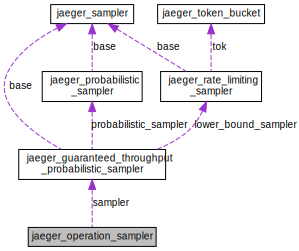
\includegraphics[width=350pt]{structjaeger__operation__sampler__coll__graph}
\end{center}
\end{figure}
\subsection*{Data Fields}
\begin{DoxyCompactItemize}
\item 
\mbox{\Hypertarget{structjaeger__operation__sampler_a4b5bd75a1b00242355c7d9094294fe5c}\label{structjaeger__operation__sampler_a4b5bd75a1b00242355c7d9094294fe5c}} 
char $\ast$ {\bfseries operation\+\_\+name}
\item 
\mbox{\Hypertarget{structjaeger__operation__sampler_a3996d2cdbbb5f6047a1e130e2ca397b5}\label{structjaeger__operation__sampler_a3996d2cdbbb5f6047a1e130e2ca397b5}} 
\mbox{\hyperlink{structjaeger__guaranteed__throughput__probabilistic__sampler}{jaeger\+\_\+guaranteed\+\_\+throughput\+\_\+probabilistic\+\_\+sampler}} {\bfseries sampler}
\end{DoxyCompactItemize}


The documentation for this struct was generated from the following file\+:\begin{DoxyCompactItemize}
\item 
jaegertracingc/\mbox{\hyperlink{sampler_8h}{sampler.\+h}}\end{DoxyCompactItemize}

\hypertarget{structjaeger__probabilistic__sampler}{}\section{jaeger\+\_\+probabilistic\+\_\+sampler Struct Reference}
\label{structjaeger__probabilistic__sampler}\index{jaeger\+\_\+probabilistic\+\_\+sampler@{jaeger\+\_\+probabilistic\+\_\+sampler}}


Collaboration diagram for jaeger\+\_\+probabilistic\+\_\+sampler\+:\nopagebreak
\begin{figure}[H]
\begin{center}
\leavevmode
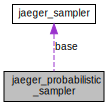
\includegraphics[width=180pt]{structjaeger__probabilistic__sampler__coll__graph}
\end{center}
\end{figure}
\subsection*{Data Fields}
\begin{DoxyCompactItemize}
\item 
\mbox{\Hypertarget{structjaeger__probabilistic__sampler_a3b25586eb505eb4991c7bc67e3d1ef40}\label{structjaeger__probabilistic__sampler_a3b25586eb505eb4991c7bc67e3d1ef40}} 
\mbox{\hyperlink{structjaeger__sampler}{jaeger\+\_\+sampler}} {\bfseries base}
\item 
\mbox{\Hypertarget{structjaeger__probabilistic__sampler_aa74aad7ba4b1803ce8a4377be9a3f79d}\label{structjaeger__probabilistic__sampler_aa74aad7ba4b1803ce8a4377be9a3f79d}} 
double {\bfseries sampling\+\_\+rate}
\end{DoxyCompactItemize}


The documentation for this struct was generated from the following file\+:\begin{DoxyCompactItemize}
\item 
jaegertracingc/\mbox{\hyperlink{sampler_8h}{sampler.\+h}}\end{DoxyCompactItemize}

\hypertarget{structjaeger__rate__limiting__sampler}{}\section{jaeger\+\_\+rate\+\_\+limiting\+\_\+sampler Struct Reference}
\label{structjaeger__rate__limiting__sampler}\index{jaeger\+\_\+rate\+\_\+limiting\+\_\+sampler@{jaeger\+\_\+rate\+\_\+limiting\+\_\+sampler}}


Collaboration diagram for jaeger\+\_\+rate\+\_\+limiting\+\_\+sampler\+:\nopagebreak
\begin{figure}[H]
\begin{center}
\leavevmode
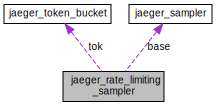
\includegraphics[width=288pt]{structjaeger__rate__limiting__sampler__coll__graph}
\end{center}
\end{figure}
\subsection*{Data Fields}
\begin{DoxyCompactItemize}
\item 
\mbox{\Hypertarget{structjaeger__rate__limiting__sampler_af8345a1a569ea3fee33a7bffa58c453a}\label{structjaeger__rate__limiting__sampler_af8345a1a569ea3fee33a7bffa58c453a}} 
\mbox{\hyperlink{structjaeger__sampler}{jaeger\+\_\+sampler}} {\bfseries base}
\item 
\mbox{\Hypertarget{structjaeger__rate__limiting__sampler_aef9553063816b15b71ac6f5efa967fee}\label{structjaeger__rate__limiting__sampler_aef9553063816b15b71ac6f5efa967fee}} 
\mbox{\hyperlink{structjaeger__token__bucket}{jaeger\+\_\+token\+\_\+bucket}} {\bfseries tok}
\item 
\mbox{\Hypertarget{structjaeger__rate__limiting__sampler_a6cfe75697a5e6a2683c7babf40db2be5}\label{structjaeger__rate__limiting__sampler_a6cfe75697a5e6a2683c7babf40db2be5}} 
double {\bfseries max\+\_\+traces\+\_\+per\+\_\+second}
\end{DoxyCompactItemize}


The documentation for this struct was generated from the following file\+:\begin{DoxyCompactItemize}
\item 
jaegertracingc/\mbox{\hyperlink{sampler_8h}{sampler.\+h}}\end{DoxyCompactItemize}

\hypertarget{structjaeger__remote__reporter}{}\section{jaeger\+\_\+remote\+\_\+reporter Struct Reference}
\label{structjaeger__remote__reporter}\index{jaeger\+\_\+remote\+\_\+reporter@{jaeger\+\_\+remote\+\_\+reporter}}


Collaboration diagram for jaeger\+\_\+remote\+\_\+reporter\+:
\nopagebreak
\begin{figure}[H]
\begin{center}
\leavevmode
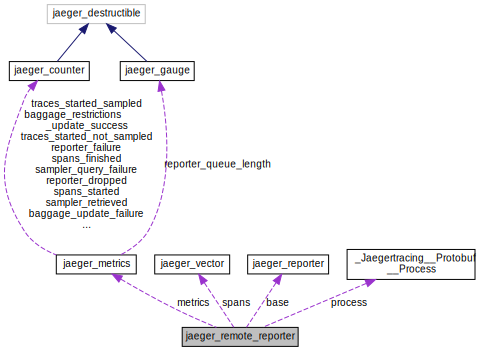
\includegraphics[width=350pt]{structjaeger__remote__reporter__coll__graph}
\end{center}
\end{figure}
\subsection*{Data Fields}
\begin{DoxyCompactItemize}
\item 
\mbox{\Hypertarget{structjaeger__remote__reporter_a89bd53b42a0b16a2e5bfa9a95d3b5e16}\label{structjaeger__remote__reporter_a89bd53b42a0b16a2e5bfa9a95d3b5e16}} 
\mbox{\hyperlink{structjaeger__reporter}{jaeger\+\_\+reporter}} {\bfseries base}
\item 
\mbox{\Hypertarget{structjaeger__remote__reporter_a4b27982db06432b478b409878547bb5f}\label{structjaeger__remote__reporter_a4b27982db06432b478b409878547bb5f}} 
int {\bfseries max\+\_\+packet\+\_\+size}
\item 
\mbox{\Hypertarget{structjaeger__remote__reporter_a6fcfeba0f020bd1f00135431e352b2d7}\label{structjaeger__remote__reporter_a6fcfeba0f020bd1f00135431e352b2d7}} 
int {\bfseries fd}
\item 
\mbox{\Hypertarget{structjaeger__remote__reporter_a8867921360be00bffacc7a930c5ee58d}\label{structjaeger__remote__reporter_a8867921360be00bffacc7a930c5ee58d}} 
\mbox{\hyperlink{structjaeger__metrics}{jaeger\+\_\+metrics}} $\ast$ {\bfseries metrics}
\item 
\mbox{\Hypertarget{structjaeger__remote__reporter_a9d5abfaa9dd79e6dc0fcffc7d56c5dd0}\label{structjaeger__remote__reporter_a9d5abfaa9dd79e6dc0fcffc7d56c5dd0}} 
\mbox{\hyperlink{struct__Jaegertracing____Protobuf____Process}{Jaegertracing\+\_\+\+\_\+\+Protobuf\+\_\+\+\_\+\+Process}} {\bfseries process}
\item 
\mbox{\Hypertarget{structjaeger__remote__reporter_a74c3e087c47a8f87b69ff599ec700bde}\label{structjaeger__remote__reporter_a74c3e087c47a8f87b69ff599ec700bde}} 
\mbox{\hyperlink{structjaeger__vector}{jaeger\+\_\+vector}} {\bfseries spans}
\item 
\mbox{\Hypertarget{structjaeger__remote__reporter_af1d5e71f259ba8abc6ebae895b7f072a}\label{structjaeger__remote__reporter_af1d5e71f259ba8abc6ebae895b7f072a}} 
struct addrinfo $\ast$ {\bfseries candidates}
\item 
\mbox{\Hypertarget{structjaeger__remote__reporter_a43710b8f44d84500a9df68002c4b3a9e}\label{structjaeger__remote__reporter_a43710b8f44d84500a9df68002c4b3a9e}} 
struct sockaddr\+\_\+in {\bfseries addr}
\item 
\mbox{\Hypertarget{structjaeger__remote__reporter_a8087ff64ca9e393c1e4054e2b9eb275c}\label{structjaeger__remote__reporter_a8087ff64ca9e393c1e4054e2b9eb275c}} 
jaeger\+\_\+mutex {\bfseries mutex}
\end{DoxyCompactItemize}


The documentation for this struct was generated from the following file\+:\begin{DoxyCompactItemize}
\item 
jaegertracingc/\mbox{\hyperlink{reporter_8h}{reporter.\+h}}\end{DoxyCompactItemize}

\hypertarget{structjaeger__remotely__controlled__sampler}{}\section{jaeger\+\_\+remotely\+\_\+controlled\+\_\+sampler Struct Reference}
\label{structjaeger__remotely__controlled__sampler}\index{jaeger\+\_\+remotely\+\_\+controlled\+\_\+sampler@{jaeger\+\_\+remotely\+\_\+controlled\+\_\+sampler}}


Collaboration diagram for jaeger\+\_\+remotely\+\_\+controlled\+\_\+sampler\+:\nopagebreak
\begin{figure}[H]
\begin{center}
\leavevmode
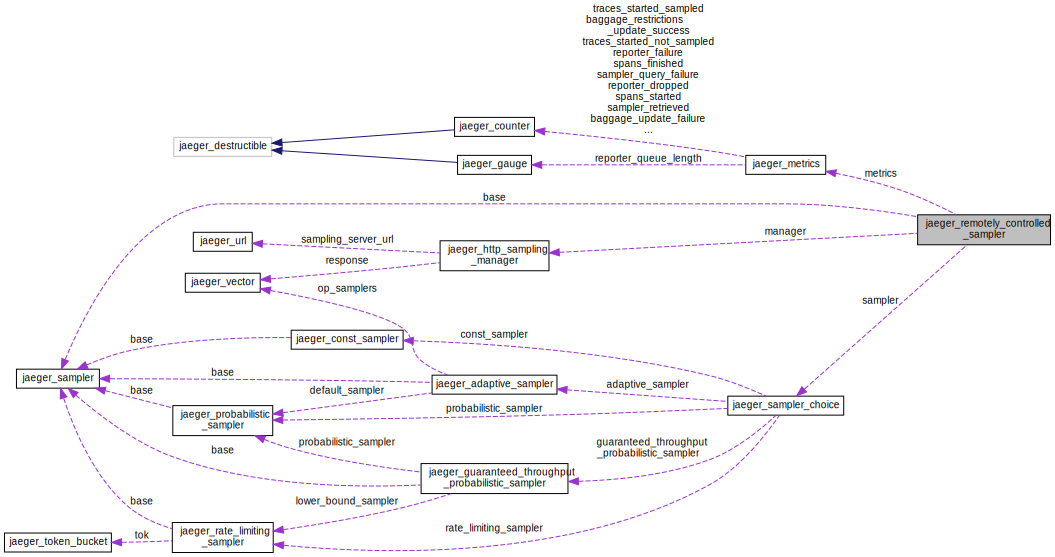
\includegraphics[width=350pt]{structjaeger__remotely__controlled__sampler__coll__graph}
\end{center}
\end{figure}
\subsection*{Data Fields}
\begin{DoxyCompactItemize}
\item 
\mbox{\Hypertarget{structjaeger__remotely__controlled__sampler_a3592c903ef829c6f6c89e6afb4478e93}\label{structjaeger__remotely__controlled__sampler_a3592c903ef829c6f6c89e6afb4478e93}} 
\mbox{\hyperlink{structjaeger__sampler}{jaeger\+\_\+sampler}} {\bfseries base}
\item 
\mbox{\Hypertarget{structjaeger__remotely__controlled__sampler_ab46de8d8bcbf5a44266ed95d497011a1}\label{structjaeger__remotely__controlled__sampler_ab46de8d8bcbf5a44266ed95d497011a1}} 
\mbox{\hyperlink{structjaeger__sampler__choice}{jaeger\+\_\+sampler\+\_\+choice}} {\bfseries sampler}
\item 
\mbox{\Hypertarget{structjaeger__remotely__controlled__sampler_a7277191696e1359eb08feee4fce054ea}\label{structjaeger__remotely__controlled__sampler_a7277191696e1359eb08feee4fce054ea}} 
int {\bfseries max\+\_\+operations}
\item 
\mbox{\Hypertarget{structjaeger__remotely__controlled__sampler_a44c9fb79d8757e90613822c6a86639e4}\label{structjaeger__remotely__controlled__sampler_a44c9fb79d8757e90613822c6a86639e4}} 
\mbox{\hyperlink{structjaeger__metrics}{jaeger\+\_\+metrics}} $\ast$ {\bfseries metrics}
\item 
\mbox{\Hypertarget{structjaeger__remotely__controlled__sampler_a9023d486696089b80f887c231c131499}\label{structjaeger__remotely__controlled__sampler_a9023d486696089b80f887c231c131499}} 
\mbox{\hyperlink{structjaeger__http__sampling__manager}{jaeger\+\_\+http\+\_\+sampling\+\_\+manager}} {\bfseries manager}
\item 
\mbox{\Hypertarget{structjaeger__remotely__controlled__sampler_ae938cdffd5db68aaeab43770b0ab385f}\label{structjaeger__remotely__controlled__sampler_ae938cdffd5db68aaeab43770b0ab385f}} 
jaeger\+\_\+mutex {\bfseries mutex}
\end{DoxyCompactItemize}


The documentation for this struct was generated from the following file\+:\begin{DoxyCompactItemize}
\item 
jaegertracingc/\mbox{\hyperlink{sampler_8h}{sampler.\+h}}\end{DoxyCompactItemize}

\hypertarget{structjaeger__reporter}{}\section{jaeger\+\_\+reporter Struct Reference}
\label{structjaeger__reporter}\index{jaeger\+\_\+reporter@{jaeger\+\_\+reporter}}
\subsection*{Data Fields}
\begin{DoxyCompactItemize}
\item 
\mbox{\Hypertarget{structjaeger__reporter_af897c2ec6ff7a5340f14008ffad9a209}\label{structjaeger__reporter_af897c2ec6ff7a5340f14008ffad9a209}} 
jaeger\+\_\+destructible {\bfseries base}
\item 
void($\ast$ \mbox{\hyperlink{structjaeger__reporter_a39f5460f19fe10f0267a6e6be240c1cc}{report}} )(struct \mbox{\hyperlink{structjaeger__reporter}{jaeger\+\_\+reporter}} $\ast$reporter, const \mbox{\hyperlink{structjaeger__span}{jaeger\+\_\+span}} $\ast$span)
\begin{DoxyCompactList}\small\item\em Report span. \end{DoxyCompactList}\item 
bool($\ast$ \mbox{\hyperlink{structjaeger__reporter_a8cfdee6e96497116c184476050b8fb13}{flush}} )(struct \mbox{\hyperlink{structjaeger__reporter}{jaeger\+\_\+reporter}} $\ast$reporter)
\begin{DoxyCompactList}\small\item\em Flush any pending spans. \end{DoxyCompactList}\end{DoxyCompactItemize}


\subsection{Field Documentation}
\mbox{\Hypertarget{structjaeger__reporter_a8cfdee6e96497116c184476050b8fb13}\label{structjaeger__reporter_a8cfdee6e96497116c184476050b8fb13}} 
\index{jaeger\+\_\+reporter@{jaeger\+\_\+reporter}!flush@{flush}}
\index{flush@{flush}!jaeger\+\_\+reporter@{jaeger\+\_\+reporter}}
\subsubsection{\texorpdfstring{flush}{flush}}
{\footnotesize\ttfamily bool($\ast$ jaeger\+\_\+reporter\+::flush) (struct \mbox{\hyperlink{structjaeger__reporter}{jaeger\+\_\+reporter}} $\ast$reporter)}



Flush any pending spans. 

Only used in remote reporter. 
\begin{DoxyParams}{Parameters}
{\em reporter} & Reporter instance. \\
\hline
\end{DoxyParams}
\begin{DoxyReturn}{Returns}
True on success, false otherwise. 
\end{DoxyReturn}
\mbox{\Hypertarget{structjaeger__reporter_a39f5460f19fe10f0267a6e6be240c1cc}\label{structjaeger__reporter_a39f5460f19fe10f0267a6e6be240c1cc}} 
\index{jaeger\+\_\+reporter@{jaeger\+\_\+reporter}!report@{report}}
\index{report@{report}!jaeger\+\_\+reporter@{jaeger\+\_\+reporter}}
\subsubsection{\texorpdfstring{report}{report}}
{\footnotesize\ttfamily void($\ast$ jaeger\+\_\+reporter\+::report) (struct \mbox{\hyperlink{structjaeger__reporter}{jaeger\+\_\+reporter}} $\ast$reporter, const \mbox{\hyperlink{structjaeger__span}{jaeger\+\_\+span}} $\ast$span)}



Report span. 


\begin{DoxyParams}{Parameters}
{\em reporter} & Reporter instance. \\
\hline
{\em span} & Span to report. \\
\hline
\end{DoxyParams}


The documentation for this struct was generated from the following file\+:\begin{DoxyCompactItemize}
\item 
jaegertracingc/\mbox{\hyperlink{reporter_8h}{reporter.\+h}}\end{DoxyCompactItemize}

\hypertarget{structjaeger__reporter__config}{}\section{jaeger\+\_\+reporter\+\_\+config Struct Reference}
\label{structjaeger__reporter__config}\index{jaeger\+\_\+reporter\+\_\+config@{jaeger\+\_\+reporter\+\_\+config}}


Reporter config.  




{\ttfamily \#include $<$jaegertracingc/options.\+h$>$}



\subsection{Detailed Description}
Reporter config. 



The documentation for this struct was generated from the following file\+:\begin{DoxyCompactItemize}
\item 
jaegertracingc/\mbox{\hyperlink{options_8h}{options.\+h}}\end{DoxyCompactItemize}

\hypertarget{structjaeger__rng}{}\section{jaeger\+\_\+rng Struct Reference}
\label{structjaeger__rng}\index{jaeger\+\_\+rng@{jaeger\+\_\+rng}}
\subsection*{Data Fields}
\begin{DoxyCompactItemize}
\item 
\mbox{\Hypertarget{structjaeger__rng_a4108a00df97a5bb2e293a60d4ee1919c}\label{structjaeger__rng_a4108a00df97a5bb2e293a60d4ee1919c}} 
jaeger\+\_\+destructible {\bfseries base}
\item 
\mbox{\Hypertarget{structjaeger__rng_a250694f288736339689044d47f3590b3}\label{structjaeger__rng_a250694f288736339689044d47f3590b3}} 
struct pcg\+\_\+state\+\_\+setseq\+\_\+64 {\bfseries state}
\end{DoxyCompactItemize}


The documentation for this struct was generated from the following file\+:\begin{DoxyCompactItemize}
\item 
jaegertracingc/internal/random.\+h\end{DoxyCompactItemize}

\hypertarget{structjaeger__sampler}{}\section{jaeger\+\_\+sampler Struct Reference}
\label{structjaeger__sampler}\index{jaeger\+\_\+sampler@{jaeger\+\_\+sampler}}
\subsection*{Data Fields}
\begin{DoxyCompactItemize}
\item 
\mbox{\Hypertarget{structjaeger__sampler_a35d9c3302303573eb173fcee2eb54485}\label{structjaeger__sampler_a35d9c3302303573eb173fcee2eb54485}} 
jaeger\+\_\+destructible {\bfseries base}
\item 
\mbox{\Hypertarget{structjaeger__sampler_a3ae4ba99898464d4c62d7c69c6d306d9}\label{structjaeger__sampler_a3ae4ba99898464d4c62d7c69c6d306d9}} 
bool($\ast$ {\bfseries is\+\_\+sampled} )(struct \mbox{\hyperlink{structjaeger__sampler}{jaeger\+\_\+sampler}} $\ast$sampler, const \mbox{\hyperlink{structjaeger__trace__id}{jaeger\+\_\+trace\+\_\+id}} $\ast$trace\+\_\+id, const char $\ast$operation, \mbox{\hyperlink{structjaeger__vector}{jaeger\+\_\+vector}} $\ast$tags)
\end{DoxyCompactItemize}


The documentation for this struct was generated from the following file\+:\begin{DoxyCompactItemize}
\item 
jaegertracingc/\mbox{\hyperlink{sampler_8h}{sampler.\+h}}\end{DoxyCompactItemize}

\hypertarget{structjaeger__sampler__choice}{}\section{jaeger\+\_\+sampler\+\_\+choice Struct Reference}
\label{structjaeger__sampler__choice}\index{jaeger\+\_\+sampler\+\_\+choice@{jaeger\+\_\+sampler\+\_\+choice}}


Collaboration diagram for jaeger\+\_\+sampler\+\_\+choice\+:\nopagebreak
\begin{figure}[H]
\begin{center}
\leavevmode
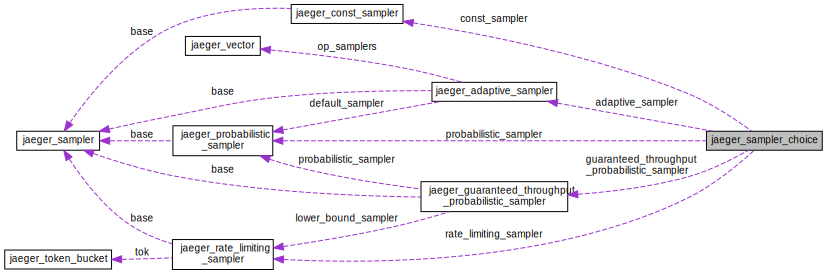
\includegraphics[width=350pt]{structjaeger__sampler__choice__coll__graph}
\end{center}
\end{figure}
\subsection*{Data Fields}
\begin{DoxyCompactItemize}
\item 
\mbox{\Hypertarget{structjaeger__sampler__choice_a408e49e3e0f0ca190a8ae9a8950eaa06}\label{structjaeger__sampler__choice_a408e49e3e0f0ca190a8ae9a8950eaa06}} 
jaeger\+\_\+sampler\+\_\+type {\bfseries type}
\item 
\mbox{\Hypertarget{structjaeger__sampler__choice_a6ca4bd899bbdbbdc8a16998c8ff2d15c}\label{structjaeger__sampler__choice_a6ca4bd899bbdbbdc8a16998c8ff2d15c}} 
\begin{tabbing}
xx\=xx\=xx\=xx\=xx\=xx\=xx\=xx\=xx\=\kill
union \{\\
\>\mbox{\hyperlink{structjaeger__const__sampler}{jaeger\_const\_sampler}} {\bfseries const\_sampler}\\
\>\mbox{\hyperlink{structjaeger__probabilistic__sampler}{jaeger\_probabilistic\_sampler}} {\bfseries probabilistic\_sampler}\\
\>\mbox{\hyperlink{structjaeger__rate__limiting__sampler}{jaeger\_rate\_limiting\_sampler}} {\bfseries rate\_limiting\_sampler}\\
\>\mbox{\hyperlink{structjaeger__guaranteed__throughput__probabilistic__sampler}{jaeger\_guaranteed\_throughput\_probabilistic\_sampler}} {\bfseries guaranteed\_throughput\_probabilistic\_sampler}\\
\>\mbox{\hyperlink{structjaeger__adaptive__sampler}{jaeger\_adaptive\_sampler}} {\bfseries adaptive\_sampler}\\
\}; \\

\end{tabbing}\end{DoxyCompactItemize}


The documentation for this struct was generated from the following file\+:\begin{DoxyCompactItemize}
\item 
jaegertracingc/\mbox{\hyperlink{sampler_8h}{sampler.\+h}}\end{DoxyCompactItemize}

\hypertarget{structjaeger__sampler__config}{}\section{jaeger\+\_\+sampler\+\_\+config Struct Reference}
\label{structjaeger__sampler__config}\index{jaeger\+\_\+sampler\+\_\+config@{jaeger\+\_\+sampler\+\_\+config}}


Sampler config.  




{\ttfamily \#include $<$jaegertracingc/options.\+h$>$}



\subsection{Detailed Description}
Sampler config. 



The documentation for this struct was generated from the following file\+:\begin{DoxyCompactItemize}
\item 
jaegertracingc/\mbox{\hyperlink{options_8h}{options.\+h}}\end{DoxyCompactItemize}

\hypertarget{structjaeger__span}{}\section{jaeger\+\_\+span Struct Reference}
\label{structjaeger__span}\index{jaeger\+\_\+span@{jaeger\+\_\+span}}


Collaboration diagram for jaeger\+\_\+span\+:\nopagebreak
\begin{figure}[H]
\begin{center}
\leavevmode
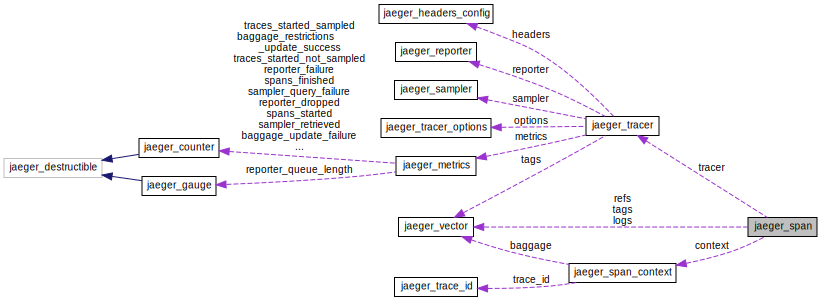
\includegraphics[width=350pt]{structjaeger__span__coll__graph}
\end{center}
\end{figure}
\subsection*{Data Fields}
\begin{DoxyCompactItemize}
\item 
opentracing\+\_\+span \mbox{\hyperlink{structjaeger__span_a4d784dc9f217e068159cccc5f0f480e9}{base}}
\begin{DoxyCompactList}\small\item\em Base class member. \end{DoxyCompactList}\item 
struct \mbox{\hyperlink{structjaeger__tracer}{jaeger\+\_\+tracer}} $\ast$ \mbox{\hyperlink{structjaeger__span_a7cff74ecb3637cba8038d0d600d4acff}{tracer}}
\begin{DoxyCompactList}\small\item\em Tracer that creates this span. \end{DoxyCompactList}\item 
\mbox{\hyperlink{structjaeger__span__context}{jaeger\+\_\+span\+\_\+context}} \mbox{\hyperlink{structjaeger__span_a2c2ee45174f03b8453d60accd018a001}{context}}
\begin{DoxyCompactList}\small\item\em Span context. \end{DoxyCompactList}\item 
char $\ast$ \mbox{\hyperlink{structjaeger__span_afacbb7789eb032da0f25933737b61093}{operation\+\_\+name}}
\begin{DoxyCompactList}\small\item\em Operation represented by this span. \end{DoxyCompactList}\item 
jaeger\+\_\+timestamp \mbox{\hyperlink{structjaeger__span_ad3c4f8aaffedbcb41697529a486d8c96}{start\+\_\+time\+\_\+system}}
\begin{DoxyCompactList}\small\item\em Start time using system clock. \end{DoxyCompactList}\item 
jaeger\+\_\+duration \mbox{\hyperlink{structjaeger__span_a5adeeb2e496220890ec3a7f5fbb69543}{start\+\_\+time\+\_\+steady}}
\begin{DoxyCompactList}\small\item\em Start time using monotonic/steady clock. \end{DoxyCompactList}\item 
jaeger\+\_\+duration \mbox{\hyperlink{structjaeger__span_a4486fea569d2256c8e33a8b445c3f4fc}{duration}}
\begin{DoxyCompactList}\small\item\em Overall duration of span (set on span finish). \end{DoxyCompactList}\item 
\mbox{\hyperlink{structjaeger__vector}{jaeger\+\_\+vector}} \mbox{\hyperlink{structjaeger__span_ae3812e107e701876ca824427ebdddbde}{tags}}
\begin{DoxyCompactList}\small\item\em Span tags. \end{DoxyCompactList}\item 
\mbox{\hyperlink{structjaeger__vector}{jaeger\+\_\+vector}} \mbox{\hyperlink{structjaeger__span_ab5b68679359d40f6821fffdbbb9cce01}{logs}}
\begin{DoxyCompactList}\small\item\em Span log records. \end{DoxyCompactList}\item 
\mbox{\hyperlink{structjaeger__vector}{jaeger\+\_\+vector}} \mbox{\hyperlink{structjaeger__span_a043c406e757c68b4c862d36d6b729cba}{refs}}
\begin{DoxyCompactList}\small\item\em Span context references (i.\+e. \end{DoxyCompactList}\item 
jaeger\+\_\+mutex \mbox{\hyperlink{structjaeger__span_a84d3f190ba0bb7106efdfe9d8e47beeb}{mutex}}
\begin{DoxyCompactList}\small\item\em Mutex to guard mutable members. \end{DoxyCompactList}\end{DoxyCompactItemize}


\subsection{Field Documentation}
\mbox{\Hypertarget{structjaeger__span_a4d784dc9f217e068159cccc5f0f480e9}\label{structjaeger__span_a4d784dc9f217e068159cccc5f0f480e9}} 
\index{jaeger\+\_\+span@{jaeger\+\_\+span}!base@{base}}
\index{base@{base}!jaeger\+\_\+span@{jaeger\+\_\+span}}
\subsubsection{\texorpdfstring{base}{base}}
{\footnotesize\ttfamily opentracing\+\_\+span jaeger\+\_\+span\+::base}



Base class member. 

\mbox{\Hypertarget{structjaeger__span_a2c2ee45174f03b8453d60accd018a001}\label{structjaeger__span_a2c2ee45174f03b8453d60accd018a001}} 
\index{jaeger\+\_\+span@{jaeger\+\_\+span}!context@{context}}
\index{context@{context}!jaeger\+\_\+span@{jaeger\+\_\+span}}
\subsubsection{\texorpdfstring{context}{context}}
{\footnotesize\ttfamily \mbox{\hyperlink{structjaeger__span__context}{jaeger\+\_\+span\+\_\+context}} jaeger\+\_\+span\+::context}



Span context. 

\mbox{\Hypertarget{structjaeger__span_a4486fea569d2256c8e33a8b445c3f4fc}\label{structjaeger__span_a4486fea569d2256c8e33a8b445c3f4fc}} 
\index{jaeger\+\_\+span@{jaeger\+\_\+span}!duration@{duration}}
\index{duration@{duration}!jaeger\+\_\+span@{jaeger\+\_\+span}}
\subsubsection{\texorpdfstring{duration}{duration}}
{\footnotesize\ttfamily jaeger\+\_\+duration jaeger\+\_\+span\+::duration}



Overall duration of span (set on span finish). 

\mbox{\Hypertarget{structjaeger__span_ab5b68679359d40f6821fffdbbb9cce01}\label{structjaeger__span_ab5b68679359d40f6821fffdbbb9cce01}} 
\index{jaeger\+\_\+span@{jaeger\+\_\+span}!logs@{logs}}
\index{logs@{logs}!jaeger\+\_\+span@{jaeger\+\_\+span}}
\subsubsection{\texorpdfstring{logs}{logs}}
{\footnotesize\ttfamily \mbox{\hyperlink{structjaeger__vector}{jaeger\+\_\+vector}} jaeger\+\_\+span\+::logs}



Span log records. 

\mbox{\Hypertarget{structjaeger__span_a84d3f190ba0bb7106efdfe9d8e47beeb}\label{structjaeger__span_a84d3f190ba0bb7106efdfe9d8e47beeb}} 
\index{jaeger\+\_\+span@{jaeger\+\_\+span}!mutex@{mutex}}
\index{mutex@{mutex}!jaeger\+\_\+span@{jaeger\+\_\+span}}
\subsubsection{\texorpdfstring{mutex}{mutex}}
{\footnotesize\ttfamily jaeger\+\_\+mutex jaeger\+\_\+span\+::mutex}



Mutex to guard mutable members. 

\mbox{\Hypertarget{structjaeger__span_afacbb7789eb032da0f25933737b61093}\label{structjaeger__span_afacbb7789eb032da0f25933737b61093}} 
\index{jaeger\+\_\+span@{jaeger\+\_\+span}!operation\+\_\+name@{operation\+\_\+name}}
\index{operation\+\_\+name@{operation\+\_\+name}!jaeger\+\_\+span@{jaeger\+\_\+span}}
\subsubsection{\texorpdfstring{operation\+\_\+name}{operation\_name}}
{\footnotesize\ttfamily char$\ast$ jaeger\+\_\+span\+::operation\+\_\+name}



Operation represented by this span. 

\mbox{\Hypertarget{structjaeger__span_a043c406e757c68b4c862d36d6b729cba}\label{structjaeger__span_a043c406e757c68b4c862d36d6b729cba}} 
\index{jaeger\+\_\+span@{jaeger\+\_\+span}!refs@{refs}}
\index{refs@{refs}!jaeger\+\_\+span@{jaeger\+\_\+span}}
\subsubsection{\texorpdfstring{refs}{refs}}
{\footnotesize\ttfamily \mbox{\hyperlink{structjaeger__vector}{jaeger\+\_\+vector}} jaeger\+\_\+span\+::refs}



Span context references (i.\+e. 

C\+H\+I\+L\+D\+\_\+\+OF and/or F\+O\+L\+L\+O\+W\+S\+\_\+\+F\+R\+OM). \mbox{\Hypertarget{structjaeger__span_a5adeeb2e496220890ec3a7f5fbb69543}\label{structjaeger__span_a5adeeb2e496220890ec3a7f5fbb69543}} 
\index{jaeger\+\_\+span@{jaeger\+\_\+span}!start\+\_\+time\+\_\+steady@{start\+\_\+time\+\_\+steady}}
\index{start\+\_\+time\+\_\+steady@{start\+\_\+time\+\_\+steady}!jaeger\+\_\+span@{jaeger\+\_\+span}}
\subsubsection{\texorpdfstring{start\+\_\+time\+\_\+steady}{start\_time\_steady}}
{\footnotesize\ttfamily jaeger\+\_\+duration jaeger\+\_\+span\+::start\+\_\+time\+\_\+steady}



Start time using monotonic/steady clock. 

\mbox{\Hypertarget{structjaeger__span_ad3c4f8aaffedbcb41697529a486d8c96}\label{structjaeger__span_ad3c4f8aaffedbcb41697529a486d8c96}} 
\index{jaeger\+\_\+span@{jaeger\+\_\+span}!start\+\_\+time\+\_\+system@{start\+\_\+time\+\_\+system}}
\index{start\+\_\+time\+\_\+system@{start\+\_\+time\+\_\+system}!jaeger\+\_\+span@{jaeger\+\_\+span}}
\subsubsection{\texorpdfstring{start\+\_\+time\+\_\+system}{start\_time\_system}}
{\footnotesize\ttfamily jaeger\+\_\+timestamp jaeger\+\_\+span\+::start\+\_\+time\+\_\+system}



Start time using system clock. 

\mbox{\Hypertarget{structjaeger__span_ae3812e107e701876ca824427ebdddbde}\label{structjaeger__span_ae3812e107e701876ca824427ebdddbde}} 
\index{jaeger\+\_\+span@{jaeger\+\_\+span}!tags@{tags}}
\index{tags@{tags}!jaeger\+\_\+span@{jaeger\+\_\+span}}
\subsubsection{\texorpdfstring{tags}{tags}}
{\footnotesize\ttfamily \mbox{\hyperlink{structjaeger__vector}{jaeger\+\_\+vector}} jaeger\+\_\+span\+::tags}



Span tags. 

\mbox{\Hypertarget{structjaeger__span_a7cff74ecb3637cba8038d0d600d4acff}\label{structjaeger__span_a7cff74ecb3637cba8038d0d600d4acff}} 
\index{jaeger\+\_\+span@{jaeger\+\_\+span}!tracer@{tracer}}
\index{tracer@{tracer}!jaeger\+\_\+span@{jaeger\+\_\+span}}
\subsubsection{\texorpdfstring{tracer}{tracer}}
{\footnotesize\ttfamily struct \mbox{\hyperlink{structjaeger__tracer}{jaeger\+\_\+tracer}}$\ast$ jaeger\+\_\+span\+::tracer}



Tracer that creates this span. 



The documentation for this struct was generated from the following file\+:\begin{DoxyCompactItemize}
\item 
jaegertracingc/\mbox{\hyperlink{span_8h}{span.\+h}}\end{DoxyCompactItemize}

\hypertarget{structjaeger__span__context}{}\section{jaeger\+\_\+span\+\_\+context Struct Reference}
\label{structjaeger__span__context}\index{jaeger\+\_\+span\+\_\+context@{jaeger\+\_\+span\+\_\+context}}


Span context represents propagated span identity and state.  




{\ttfamily \#include $<$jaegertracingc/span.\+h$>$}



Collaboration diagram for jaeger\+\_\+span\+\_\+context\+:\nopagebreak
\begin{figure}[H]
\begin{center}
\leavevmode
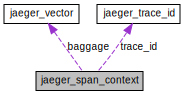
\includegraphics[width=310pt]{structjaeger__span__context__coll__graph}
\end{center}
\end{figure}
\subsection*{Data Fields}
\begin{DoxyCompactItemize}
\item 
opentracing\+\_\+span\+\_\+context \mbox{\hyperlink{structjaeger__span__context_a306504cd5d3064edc49c70e8d485a067}{base}}
\begin{DoxyCompactList}\small\item\em Base class member. \end{DoxyCompactList}\item 
\mbox{\hyperlink{structjaeger__trace__id}{jaeger\+\_\+trace\+\_\+id}} \mbox{\hyperlink{structjaeger__span__context_aecace9cbf8c8432cb8c2f5d5dc65b994}{trace\+\_\+id}}
\begin{DoxyCompactList}\small\item\em Trace ID of the trace containing this span. \end{DoxyCompactList}\item 
uint64\+\_\+t \mbox{\hyperlink{structjaeger__span__context_ad78982af52840b14a8bee7d3404755d3}{span\+\_\+id}}
\begin{DoxyCompactList}\small\item\em Randomly generated unique ID. \end{DoxyCompactList}\item 
uint64\+\_\+t \mbox{\hyperlink{structjaeger__span__context_a66ebaca50e8853b5fab9d4ebe82cfb32}{parent\+\_\+id}}
\begin{DoxyCompactList}\small\item\em Span ID of parent span. \end{DoxyCompactList}\item 
uint8\+\_\+t \mbox{\hyperlink{structjaeger__span__context_a7b79bf9f7994b640a154665cce75ec68}{flags}}
\begin{DoxyCompactList}\small\item\em Sampling flags. \end{DoxyCompactList}\item 
\mbox{\hyperlink{structjaeger__hashtable}{jaeger\+\_\+hashtable}} \mbox{\hyperlink{structjaeger__span__context_aedfb64b810e041a807dd6e0ea8274215}{baggage}}
\begin{DoxyCompactList}\small\item\em Key-\/value pairs that are propagated along with the span. \end{DoxyCompactList}\item 
char $\ast$ \mbox{\hyperlink{structjaeger__span__context_ac20ee048f523b07af732d686797fed17}{debug\+\_\+id}}
\begin{DoxyCompactList}\small\item\em Can be set to correlation ID when the context is being extracted from a carrier. \end{DoxyCompactList}\item 
jaeger\+\_\+mutex \mbox{\hyperlink{structjaeger__span__context_a56712a12a4461df451f26c91cad7a3e9}{mutex}}
\begin{DoxyCompactList}\small\item\em Lock to protect mutable members. \end{DoxyCompactList}\end{DoxyCompactItemize}


\subsection{Detailed Description}
Span context represents propagated span identity and state. 

\subsection{Field Documentation}
\mbox{\Hypertarget{structjaeger__span__context_aedfb64b810e041a807dd6e0ea8274215}\label{structjaeger__span__context_aedfb64b810e041a807dd6e0ea8274215}} 
\index{jaeger\+\_\+span\+\_\+context@{jaeger\+\_\+span\+\_\+context}!baggage@{baggage}}
\index{baggage@{baggage}!jaeger\+\_\+span\+\_\+context@{jaeger\+\_\+span\+\_\+context}}
\subsubsection{\texorpdfstring{baggage}{baggage}}
{\footnotesize\ttfamily \mbox{\hyperlink{structjaeger__hashtable}{jaeger\+\_\+hashtable}} jaeger\+\_\+span\+\_\+context\+::baggage}



Key-\/value pairs that are propagated along with the span. 

\mbox{\Hypertarget{structjaeger__span__context_a306504cd5d3064edc49c70e8d485a067}\label{structjaeger__span__context_a306504cd5d3064edc49c70e8d485a067}} 
\index{jaeger\+\_\+span\+\_\+context@{jaeger\+\_\+span\+\_\+context}!base@{base}}
\index{base@{base}!jaeger\+\_\+span\+\_\+context@{jaeger\+\_\+span\+\_\+context}}
\subsubsection{\texorpdfstring{base}{base}}
{\footnotesize\ttfamily opentracing\+\_\+span\+\_\+context jaeger\+\_\+span\+\_\+context\+::base}



Base class member. 

\mbox{\Hypertarget{structjaeger__span__context_ac20ee048f523b07af732d686797fed17}\label{structjaeger__span__context_ac20ee048f523b07af732d686797fed17}} 
\index{jaeger\+\_\+span\+\_\+context@{jaeger\+\_\+span\+\_\+context}!debug\+\_\+id@{debug\+\_\+id}}
\index{debug\+\_\+id@{debug\+\_\+id}!jaeger\+\_\+span\+\_\+context@{jaeger\+\_\+span\+\_\+context}}
\subsubsection{\texorpdfstring{debug\+\_\+id}{debug\_id}}
{\footnotesize\ttfamily char$\ast$ jaeger\+\_\+span\+\_\+context\+::debug\+\_\+id}



Can be set to correlation ID when the context is being extracted from a carrier. 

\begin{DoxySeeAlso}{See also}
J\+A\+E\+G\+E\+R\+T\+R\+A\+C\+I\+N\+G\+C\+\_\+\+D\+E\+B\+U\+G\+\_\+\+H\+E\+A\+D\+ER 
\end{DoxySeeAlso}
\mbox{\Hypertarget{structjaeger__span__context_a7b79bf9f7994b640a154665cce75ec68}\label{structjaeger__span__context_a7b79bf9f7994b640a154665cce75ec68}} 
\index{jaeger\+\_\+span\+\_\+context@{jaeger\+\_\+span\+\_\+context}!flags@{flags}}
\index{flags@{flags}!jaeger\+\_\+span\+\_\+context@{jaeger\+\_\+span\+\_\+context}}
\subsubsection{\texorpdfstring{flags}{flags}}
{\footnotesize\ttfamily uint8\+\_\+t jaeger\+\_\+span\+\_\+context\+::flags}



Sampling flags. 

\mbox{\Hypertarget{structjaeger__span__context_a56712a12a4461df451f26c91cad7a3e9}\label{structjaeger__span__context_a56712a12a4461df451f26c91cad7a3e9}} 
\index{jaeger\+\_\+span\+\_\+context@{jaeger\+\_\+span\+\_\+context}!mutex@{mutex}}
\index{mutex@{mutex}!jaeger\+\_\+span\+\_\+context@{jaeger\+\_\+span\+\_\+context}}
\subsubsection{\texorpdfstring{mutex}{mutex}}
{\footnotesize\ttfamily jaeger\+\_\+mutex jaeger\+\_\+span\+\_\+context\+::mutex}



Lock to protect mutable members. 

\begin{DoxySeeAlso}{See also}
\mbox{\hyperlink{structjaeger__span__context_aedfb64b810e041a807dd6e0ea8274215}{baggage}} 
\end{DoxySeeAlso}
\mbox{\Hypertarget{structjaeger__span__context_a66ebaca50e8853b5fab9d4ebe82cfb32}\label{structjaeger__span__context_a66ebaca50e8853b5fab9d4ebe82cfb32}} 
\index{jaeger\+\_\+span\+\_\+context@{jaeger\+\_\+span\+\_\+context}!parent\+\_\+id@{parent\+\_\+id}}
\index{parent\+\_\+id@{parent\+\_\+id}!jaeger\+\_\+span\+\_\+context@{jaeger\+\_\+span\+\_\+context}}
\subsubsection{\texorpdfstring{parent\+\_\+id}{parent\_id}}
{\footnotesize\ttfamily uint64\+\_\+t jaeger\+\_\+span\+\_\+context\+::parent\+\_\+id}



Span ID of parent span. 

Parent ID of zero represents root span. \mbox{\Hypertarget{structjaeger__span__context_ad78982af52840b14a8bee7d3404755d3}\label{structjaeger__span__context_ad78982af52840b14a8bee7d3404755d3}} 
\index{jaeger\+\_\+span\+\_\+context@{jaeger\+\_\+span\+\_\+context}!span\+\_\+id@{span\+\_\+id}}
\index{span\+\_\+id@{span\+\_\+id}!jaeger\+\_\+span\+\_\+context@{jaeger\+\_\+span\+\_\+context}}
\subsubsection{\texorpdfstring{span\+\_\+id}{span\_id}}
{\footnotesize\ttfamily uint64\+\_\+t jaeger\+\_\+span\+\_\+context\+::span\+\_\+id}



Randomly generated unique ID. 

Must be unique within its trace, but not necessarily globally unique. \mbox{\Hypertarget{structjaeger__span__context_aecace9cbf8c8432cb8c2f5d5dc65b994}\label{structjaeger__span__context_aecace9cbf8c8432cb8c2f5d5dc65b994}} 
\index{jaeger\+\_\+span\+\_\+context@{jaeger\+\_\+span\+\_\+context}!trace\+\_\+id@{trace\+\_\+id}}
\index{trace\+\_\+id@{trace\+\_\+id}!jaeger\+\_\+span\+\_\+context@{jaeger\+\_\+span\+\_\+context}}
\subsubsection{\texorpdfstring{trace\+\_\+id}{trace\_id}}
{\footnotesize\ttfamily \mbox{\hyperlink{structjaeger__trace__id}{jaeger\+\_\+trace\+\_\+id}} jaeger\+\_\+span\+\_\+context\+::trace\+\_\+id}



Trace ID of the trace containing this span. 



The documentation for this struct was generated from the following file\+:\begin{DoxyCompactItemize}
\item 
jaegertracingc/\mbox{\hyperlink{span_8h}{span.\+h}}\end{DoxyCompactItemize}

\hypertarget{structjaeger__span__ref}{}\section{jaeger\+\_\+span\+\_\+ref Struct Reference}
\label{structjaeger__span__ref}\index{jaeger\+\_\+span\+\_\+ref@{jaeger\+\_\+span\+\_\+ref}}


Collaboration diagram for jaeger\+\_\+span\+\_\+ref\+:\nopagebreak
\begin{figure}[H]
\begin{center}
\leavevmode
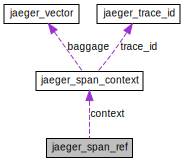
\includegraphics[width=310pt]{structjaeger__span__ref__coll__graph}
\end{center}
\end{figure}
\subsection*{Data Fields}
\begin{DoxyCompactItemize}
\item 
\mbox{\Hypertarget{structjaeger__span__ref_a35959d629d46786a74f76844f39cd18a}\label{structjaeger__span__ref_a35959d629d46786a74f76844f39cd18a}} 
\mbox{\hyperlink{structjaeger__span__context}{jaeger\+\_\+span\+\_\+context}} {\bfseries context}
\item 
\mbox{\Hypertarget{structjaeger__span__ref_a465808f3eb23d6d5f1b0672d0f533305}\label{structjaeger__span__ref_a465808f3eb23d6d5f1b0672d0f533305}} 
jaeger\+\_\+span\+\_\+ref\+\_\+type {\bfseries type}
\end{DoxyCompactItemize}


The documentation for this struct was generated from the following file\+:\begin{DoxyCompactItemize}
\item 
jaegertracingc/\mbox{\hyperlink{span_8h}{span.\+h}}\end{DoxyCompactItemize}

\hypertarget{structjaeger__thread__local}{}\section{jaeger\+\_\+thread\+\_\+local Struct Reference}
\label{structjaeger__thread__local}\index{jaeger\+\_\+thread\+\_\+local@{jaeger\+\_\+thread\+\_\+local}}
\subsection*{Data Fields}
\begin{DoxyCompactItemize}
\item 
\mbox{\Hypertarget{structjaeger__thread__local_a5c2963fb2a23a5d7a7c74cd6781fd6a9}\label{structjaeger__thread__local_a5c2963fb2a23a5d7a7c74cd6781fd6a9}} 
pthread\+\_\+key\+\_\+t {\bfseries key}
\item 
\mbox{\Hypertarget{structjaeger__thread__local_a7c96bea598a3e648891d6499f2b02038}\label{structjaeger__thread__local_a7c96bea598a3e648891d6499f2b02038}} 
bool {\bfseries initialized}
\end{DoxyCompactItemize}


The documentation for this struct was generated from the following file\+:\begin{DoxyCompactItemize}
\item 
jaegertracingc/\mbox{\hyperlink{threading_8h}{threading.\+h}}\end{DoxyCompactItemize}

\hypertarget{structjaeger__token__bucket}{}\section{jaeger\+\_\+token\+\_\+bucket Struct Reference}
\label{structjaeger__token__bucket}\index{jaeger\+\_\+token\+\_\+bucket@{jaeger\+\_\+token\+\_\+bucket}}
\subsection*{Data Fields}
\begin{DoxyCompactItemize}
\item 
\mbox{\Hypertarget{structjaeger__token__bucket_a6c34455efc70e94d5723c4883700234b}\label{structjaeger__token__bucket_a6c34455efc70e94d5723c4883700234b}} 
double {\bfseries credits\+\_\+per\+\_\+second}
\item 
\mbox{\Hypertarget{structjaeger__token__bucket_a9d19702f34ee0d6f287e6bc16278f181}\label{structjaeger__token__bucket_a9d19702f34ee0d6f287e6bc16278f181}} 
double {\bfseries max\+\_\+balance}
\item 
\mbox{\Hypertarget{structjaeger__token__bucket_a903d00af2a3538eebb35470b8cc85f74}\label{structjaeger__token__bucket_a903d00af2a3538eebb35470b8cc85f74}} 
double {\bfseries balance}
\item 
\mbox{\Hypertarget{structjaeger__token__bucket_a1e740e19399b191389a7bc17ab9143d5}\label{structjaeger__token__bucket_a1e740e19399b191389a7bc17ab9143d5}} 
jaeger\+\_\+duration {\bfseries last\+\_\+tick}
\end{DoxyCompactItemize}


The documentation for this struct was generated from the following file\+:\begin{DoxyCompactItemize}
\item 
jaegertracingc/\mbox{\hyperlink{token__bucket_8h}{token\+\_\+bucket.\+h}}\end{DoxyCompactItemize}

\hypertarget{structjaeger__trace__id}{}\section{jaeger\+\_\+trace\+\_\+id Struct Reference}
\label{structjaeger__trace__id}\index{jaeger\+\_\+trace\+\_\+id@{jaeger\+\_\+trace\+\_\+id}}


128 bit unique ID for a given trace.  




{\ttfamily \#include $<$jaegertracingc/trace\+\_\+id.\+h$>$}

\subsection*{Data Fields}
\begin{DoxyCompactItemize}
\item 
uint64\+\_\+t \mbox{\hyperlink{structjaeger__trace__id_a9dd33226f6827ef126be0857416f7043}{high}}
\begin{DoxyCompactList}\small\item\em Upper 64 bits of the trace ID. \end{DoxyCompactList}\item 
uint64\+\_\+t \mbox{\hyperlink{structjaeger__trace__id_af6a2c57fe8c53b8a1dbe114a757ab3b7}{low}}
\begin{DoxyCompactList}\small\item\em Lower 64 bits of the trace ID. \end{DoxyCompactList}\end{DoxyCompactItemize}


\subsection{Detailed Description}
128 bit unique ID for a given trace. 



\subsection{Field Documentation}
\mbox{\Hypertarget{structjaeger__trace__id_a9dd33226f6827ef126be0857416f7043}\label{structjaeger__trace__id_a9dd33226f6827ef126be0857416f7043}} 
\index{jaeger\+\_\+trace\+\_\+id@{jaeger\+\_\+trace\+\_\+id}!high@{high}}
\index{high@{high}!jaeger\+\_\+trace\+\_\+id@{jaeger\+\_\+trace\+\_\+id}}
\subsubsection{\texorpdfstring{high}{high}}
{\footnotesize\ttfamily uint64\+\_\+t jaeger\+\_\+trace\+\_\+id\+::high}



Upper 64 bits of the trace ID. 

\mbox{\Hypertarget{structjaeger__trace__id_af6a2c57fe8c53b8a1dbe114a757ab3b7}\label{structjaeger__trace__id_af6a2c57fe8c53b8a1dbe114a757ab3b7}} 
\index{jaeger\+\_\+trace\+\_\+id@{jaeger\+\_\+trace\+\_\+id}!low@{low}}
\index{low@{low}!jaeger\+\_\+trace\+\_\+id@{jaeger\+\_\+trace\+\_\+id}}
\subsubsection{\texorpdfstring{low}{low}}
{\footnotesize\ttfamily uint64\+\_\+t jaeger\+\_\+trace\+\_\+id\+::low}



Lower 64 bits of the trace ID. 



The documentation for this struct was generated from the following file\+:\begin{DoxyCompactItemize}
\item 
jaegertracingc/\mbox{\hyperlink{trace__id_8h}{trace\+\_\+id.\+h}}\end{DoxyCompactItemize}

\hypertarget{structjaeger__tracer}{}\section{jaeger\+\_\+tracer Struct Reference}
\label{structjaeger__tracer}\index{jaeger\+\_\+tracer@{jaeger\+\_\+tracer}}


Tracer implementation.  




{\ttfamily \#include $<$jaegertracingc/tracer.\+h$>$}



Collaboration diagram for jaeger\+\_\+tracer\+:\nopagebreak
\begin{figure}[H]
\begin{center}
\leavevmode
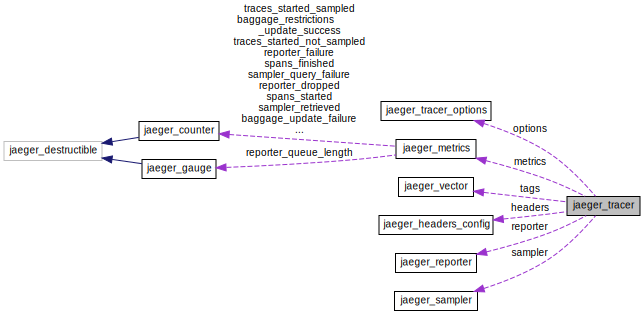
\includegraphics[width=350pt]{structjaeger__tracer__coll__graph}
\end{center}
\end{figure}
\subsection*{Data Fields}
\begin{DoxyCompactItemize}
\item 
opentracing\+\_\+tracer \mbox{\hyperlink{structjaeger__tracer_a0cb44e6988002ef749df0f3a44a8c6fc}{base}}
\begin{DoxyCompactList}\small\item\em Base class instance. \end{DoxyCompactList}\item 
char $\ast$ \mbox{\hyperlink{structjaeger__tracer_a2f266f1e4c48383eb3460f3a042a14c3}{service\+\_\+name}}
\begin{DoxyCompactList}\small\item\em Name of the current service. \end{DoxyCompactList}\item 
\mbox{\hyperlink{structjaeger__metrics}{jaeger\+\_\+metrics}} $\ast$ \mbox{\hyperlink{structjaeger__tracer_a1dd0f33dd401acec1affee5e74e4ce1a}{metrics}}
\begin{DoxyCompactList}\small\item\em Metrics object to use in tracer. \end{DoxyCompactList}\item 
\mbox{\hyperlink{structjaeger__sampler}{jaeger\+\_\+sampler}} $\ast$ \mbox{\hyperlink{structjaeger__tracer_a988ac3ac189df44661bedc45d55b56c8}{sampler}}
\begin{DoxyCompactList}\small\item\em Sampler to select spans for tracing. \end{DoxyCompactList}\item 
\mbox{\hyperlink{structjaeger__reporter}{jaeger\+\_\+reporter}} $\ast$ \mbox{\hyperlink{structjaeger__tracer_ade315b4e4a1bef2bbccee5f9e8bb4f3d}{reporter}}
\begin{DoxyCompactList}\small\item\em Reporter to handle spans after they are completed. \end{DoxyCompactList}\item 
\mbox{\hyperlink{structjaeger__tracer__options}{jaeger\+\_\+tracer\+\_\+options}} \mbox{\hyperlink{structjaeger__tracer_ac75ef3b2257e8ba0eea1dfb8828ec193}{options}}
\begin{DoxyCompactList}\small\item\em Custom options passed into the tracer at construction. \end{DoxyCompactList}\item 
\mbox{\hyperlink{structjaeger__headers__config}{jaeger\+\_\+headers\+\_\+config}} \mbox{\hyperlink{structjaeger__tracer_adfcabc1df77962918610907797229e0d}{headers}}
\begin{DoxyCompactList}\small\item\em Headers config for span propagation. \end{DoxyCompactList}\item 
\mbox{\hyperlink{structjaeger__vector}{jaeger\+\_\+vector}} \mbox{\hyperlink{structjaeger__tracer_a6e776148ebfb95dc49bbf018b58841e5}{tags}}
\begin{DoxyCompactList}\small\item\em Tags to store metadata about the current process (i.\+e. \end{DoxyCompactList}\item 
\mbox{\Hypertarget{structjaeger__tracer_a61b99abb9c413a2a36c3d8b77050c3e6}\label{structjaeger__tracer_a61b99abb9c413a2a36c3d8b77050c3e6}} 
\begin{tabbing}
xx\=xx\=xx\=xx\=xx\=xx\=xx\=xx\=xx\=\kill
struct \{\\
\>bool \mbox{\hyperlink{structjaeger__tracer_ad829501be0454a1ede7de6448d923705}{metrics}}\\
\>\>{\em True if metrics is heap-\/allocated, false otherwise. }\\
\>bool \mbox{\hyperlink{structjaeger__tracer_a77efb5d19028805e0531787e7059dd39}{sampler}}\\
\>\>{\em True if sampler is heap-\/allocated, false otherwise. }\\
\>bool \mbox{\hyperlink{structjaeger__tracer_a7d7447ff17fbafd8adf6e68dfba758e9}{reporter}}\\
\>\>{\em True if reporter is heap-\/allocated, false otherwise. }\\
\} \mbox{\hyperlink{structjaeger__tracer_a61b99abb9c413a2a36c3d8b77050c3e6}{allocated}}\\

\end{tabbing}\begin{DoxyCompactList}\small\item\em Flags to keep track of the members that were heap-\/allocated and must be freed by the tracer. \end{DoxyCompactList}\end{DoxyCompactItemize}


\subsection{Detailed Description}
Tracer implementation. 

\subsection{Field Documentation}
\mbox{\Hypertarget{structjaeger__tracer_a0cb44e6988002ef749df0f3a44a8c6fc}\label{structjaeger__tracer_a0cb44e6988002ef749df0f3a44a8c6fc}} 
\index{jaeger\+\_\+tracer@{jaeger\+\_\+tracer}!base@{base}}
\index{base@{base}!jaeger\+\_\+tracer@{jaeger\+\_\+tracer}}
\subsubsection{\texorpdfstring{base}{base}}
{\footnotesize\ttfamily opentracing\+\_\+tracer jaeger\+\_\+tracer\+::base}



Base class instance. 

\mbox{\Hypertarget{structjaeger__tracer_adfcabc1df77962918610907797229e0d}\label{structjaeger__tracer_adfcabc1df77962918610907797229e0d}} 
\index{jaeger\+\_\+tracer@{jaeger\+\_\+tracer}!headers@{headers}}
\index{headers@{headers}!jaeger\+\_\+tracer@{jaeger\+\_\+tracer}}
\subsubsection{\texorpdfstring{headers}{headers}}
{\footnotesize\ttfamily \mbox{\hyperlink{structjaeger__headers__config}{jaeger\+\_\+headers\+\_\+config}} jaeger\+\_\+tracer\+::headers}



Headers config for span propagation. 

\begin{DoxySeeAlso}{See also}
\mbox{\hyperlink{structjaeger__headers__config}{jaeger\+\_\+headers\+\_\+config}} 
\end{DoxySeeAlso}
\mbox{\Hypertarget{structjaeger__tracer_a1dd0f33dd401acec1affee5e74e4ce1a}\label{structjaeger__tracer_a1dd0f33dd401acec1affee5e74e4ce1a}} 
\index{jaeger\+\_\+tracer@{jaeger\+\_\+tracer}!metrics@{metrics}}
\index{metrics@{metrics}!jaeger\+\_\+tracer@{jaeger\+\_\+tracer}}
\subsubsection{\texorpdfstring{metrics}{metrics}\hspace{0.1cm}{\footnotesize\ttfamily [1/2]}}
{\footnotesize\ttfamily \mbox{\hyperlink{structjaeger__metrics}{jaeger\+\_\+metrics}}$\ast$ jaeger\+\_\+tracer\+::metrics}



Metrics object to use in tracer. 

\begin{DoxySeeAlso}{See also}
\mbox{\hyperlink{structjaeger__metrics}{jaeger\+\_\+metrics}} 
\end{DoxySeeAlso}
\mbox{\Hypertarget{structjaeger__tracer_ad829501be0454a1ede7de6448d923705}\label{structjaeger__tracer_ad829501be0454a1ede7de6448d923705}} 
\index{jaeger\+\_\+tracer@{jaeger\+\_\+tracer}!metrics@{metrics}}
\index{metrics@{metrics}!jaeger\+\_\+tracer@{jaeger\+\_\+tracer}}
\subsubsection{\texorpdfstring{metrics}{metrics}\hspace{0.1cm}{\footnotesize\ttfamily [2/2]}}
{\footnotesize\ttfamily bool jaeger\+\_\+tracer\+::metrics}



True if metrics is heap-\/allocated, false otherwise. 

\mbox{\Hypertarget{structjaeger__tracer_ac75ef3b2257e8ba0eea1dfb8828ec193}\label{structjaeger__tracer_ac75ef3b2257e8ba0eea1dfb8828ec193}} 
\index{jaeger\+\_\+tracer@{jaeger\+\_\+tracer}!options@{options}}
\index{options@{options}!jaeger\+\_\+tracer@{jaeger\+\_\+tracer}}
\subsubsection{\texorpdfstring{options}{options}}
{\footnotesize\ttfamily \mbox{\hyperlink{structjaeger__tracer__options}{jaeger\+\_\+tracer\+\_\+options}} jaeger\+\_\+tracer\+::options}



Custom options passed into the tracer at construction. 

\begin{DoxySeeAlso}{See also}
\mbox{\hyperlink{structjaeger__tracer__options}{jaeger\+\_\+tracer\+\_\+options}} 

\mbox{\hyperlink{tracer_8h_a71950927a6d00a35e261c342349b62ec}{jaeger\+\_\+tracer\+\_\+init()}} 
\end{DoxySeeAlso}
\mbox{\Hypertarget{structjaeger__tracer_ade315b4e4a1bef2bbccee5f9e8bb4f3d}\label{structjaeger__tracer_ade315b4e4a1bef2bbccee5f9e8bb4f3d}} 
\index{jaeger\+\_\+tracer@{jaeger\+\_\+tracer}!reporter@{reporter}}
\index{reporter@{reporter}!jaeger\+\_\+tracer@{jaeger\+\_\+tracer}}
\subsubsection{\texorpdfstring{reporter}{reporter}\hspace{0.1cm}{\footnotesize\ttfamily [1/2]}}
{\footnotesize\ttfamily \mbox{\hyperlink{structjaeger__reporter}{jaeger\+\_\+reporter}}$\ast$ jaeger\+\_\+tracer\+::reporter}



Reporter to handle spans after they are completed. 

\begin{DoxySeeAlso}{See also}
\mbox{\hyperlink{structjaeger__reporter}{jaeger\+\_\+reporter}} 
\end{DoxySeeAlso}
\mbox{\Hypertarget{structjaeger__tracer_a7d7447ff17fbafd8adf6e68dfba758e9}\label{structjaeger__tracer_a7d7447ff17fbafd8adf6e68dfba758e9}} 
\index{jaeger\+\_\+tracer@{jaeger\+\_\+tracer}!reporter@{reporter}}
\index{reporter@{reporter}!jaeger\+\_\+tracer@{jaeger\+\_\+tracer}}
\subsubsection{\texorpdfstring{reporter}{reporter}\hspace{0.1cm}{\footnotesize\ttfamily [2/2]}}
{\footnotesize\ttfamily bool jaeger\+\_\+tracer\+::reporter}



True if reporter is heap-\/allocated, false otherwise. 

\mbox{\Hypertarget{structjaeger__tracer_a988ac3ac189df44661bedc45d55b56c8}\label{structjaeger__tracer_a988ac3ac189df44661bedc45d55b56c8}} 
\index{jaeger\+\_\+tracer@{jaeger\+\_\+tracer}!sampler@{sampler}}
\index{sampler@{sampler}!jaeger\+\_\+tracer@{jaeger\+\_\+tracer}}
\subsubsection{\texorpdfstring{sampler}{sampler}\hspace{0.1cm}{\footnotesize\ttfamily [1/2]}}
{\footnotesize\ttfamily \mbox{\hyperlink{structjaeger__sampler}{jaeger\+\_\+sampler}}$\ast$ jaeger\+\_\+tracer\+::sampler}



Sampler to select spans for tracing. 

\begin{DoxySeeAlso}{See also}
\mbox{\hyperlink{structjaeger__sampler}{jaeger\+\_\+sampler}} 
\end{DoxySeeAlso}
\mbox{\Hypertarget{structjaeger__tracer_a77efb5d19028805e0531787e7059dd39}\label{structjaeger__tracer_a77efb5d19028805e0531787e7059dd39}} 
\index{jaeger\+\_\+tracer@{jaeger\+\_\+tracer}!sampler@{sampler}}
\index{sampler@{sampler}!jaeger\+\_\+tracer@{jaeger\+\_\+tracer}}
\subsubsection{\texorpdfstring{sampler}{sampler}\hspace{0.1cm}{\footnotesize\ttfamily [2/2]}}
{\footnotesize\ttfamily bool jaeger\+\_\+tracer\+::sampler}



True if sampler is heap-\/allocated, false otherwise. 

\mbox{\Hypertarget{structjaeger__tracer_a2f266f1e4c48383eb3460f3a042a14c3}\label{structjaeger__tracer_a2f266f1e4c48383eb3460f3a042a14c3}} 
\index{jaeger\+\_\+tracer@{jaeger\+\_\+tracer}!service\+\_\+name@{service\+\_\+name}}
\index{service\+\_\+name@{service\+\_\+name}!jaeger\+\_\+tracer@{jaeger\+\_\+tracer}}
\subsubsection{\texorpdfstring{service\+\_\+name}{service\_name}}
{\footnotesize\ttfamily char$\ast$ jaeger\+\_\+tracer\+::service\+\_\+name}



Name of the current service. 

\mbox{\Hypertarget{structjaeger__tracer_a6e776148ebfb95dc49bbf018b58841e5}\label{structjaeger__tracer_a6e776148ebfb95dc49bbf018b58841e5}} 
\index{jaeger\+\_\+tracer@{jaeger\+\_\+tracer}!tags@{tags}}
\index{tags@{tags}!jaeger\+\_\+tracer@{jaeger\+\_\+tracer}}
\subsubsection{\texorpdfstring{tags}{tags}}
{\footnotesize\ttfamily \mbox{\hyperlink{structjaeger__vector}{jaeger\+\_\+vector}} jaeger\+\_\+tracer\+::tags}



Tags to store metadata about the current process (i.\+e. 

hostname, client version, etc.). 

The documentation for this struct was generated from the following file\+:\begin{DoxyCompactItemize}
\item 
jaegertracingc/\mbox{\hyperlink{tracer_8h}{tracer.\+h}}\end{DoxyCompactItemize}

\hypertarget{structjaeger__tracer__options}{}\section{jaeger\+\_\+tracer\+\_\+options Struct Reference}
\label{structjaeger__tracer__options}\index{jaeger\+\_\+tracer\+\_\+options@{jaeger\+\_\+tracer\+\_\+options}}


Options that can be used to customize the tracer.  




{\ttfamily \#include $<$jaegertracingc/tracer.\+h$>$}

\subsection*{Data Fields}
\begin{DoxyCompactItemize}
\item 
bool \mbox{\hyperlink{structjaeger__tracer__options_a32b273ee8cdf9219ef434cca6038ae9e}{gen\+\_\+128\+\_\+bit}}
\begin{DoxyCompactList}\small\item\em Whether to generate a 128 bit trace ID or leave high bits as zero. \end{DoxyCompactList}\end{DoxyCompactItemize}


\subsection{Detailed Description}
Options that can be used to customize the tracer. 

\subsection{Field Documentation}
\mbox{\Hypertarget{structjaeger__tracer__options_a32b273ee8cdf9219ef434cca6038ae9e}\label{structjaeger__tracer__options_a32b273ee8cdf9219ef434cca6038ae9e}} 
\index{jaeger\+\_\+tracer\+\_\+options@{jaeger\+\_\+tracer\+\_\+options}!gen\+\_\+128\+\_\+bit@{gen\+\_\+128\+\_\+bit}}
\index{gen\+\_\+128\+\_\+bit@{gen\+\_\+128\+\_\+bit}!jaeger\+\_\+tracer\+\_\+options@{jaeger\+\_\+tracer\+\_\+options}}
\subsubsection{\texorpdfstring{gen\+\_\+128\+\_\+bit}{gen\_128\_bit}}
{\footnotesize\ttfamily bool jaeger\+\_\+tracer\+\_\+options\+::gen\+\_\+128\+\_\+bit}



Whether to generate a 128 bit trace ID or leave high bits as zero. 

\begin{DoxySeeAlso}{See also}
\mbox{\hyperlink{structjaeger__trace__id}{jaeger\+\_\+trace\+\_\+id}} 
\end{DoxySeeAlso}


The documentation for this struct was generated from the following file\+:\begin{DoxyCompactItemize}
\item 
jaegertracingc/\mbox{\hyperlink{tracer_8h}{tracer.\+h}}\end{DoxyCompactItemize}

\hypertarget{structjaeger__url}{}\section{jaeger\+\_\+url Struct Reference}
\label{structjaeger__url}\index{jaeger\+\_\+url@{jaeger\+\_\+url}}
\subsection*{Data Fields}
\begin{DoxyCompactItemize}
\item 
\mbox{\Hypertarget{structjaeger__url_ac5b9682a87171c2a3ae1436c87f6f7ae}\label{structjaeger__url_ac5b9682a87171c2a3ae1436c87f6f7ae}} 
char $\ast$ {\bfseries str}
\item 
\mbox{\Hypertarget{structjaeger__url_a4a23047f8c55abe2757c3f251cb62991}\label{structjaeger__url_a4a23047f8c55abe2757c3f251cb62991}} 
struct http\+\_\+parser\+\_\+url {\bfseries parts}
\end{DoxyCompactItemize}


The documentation for this struct was generated from the following file\+:\begin{DoxyCompactItemize}
\item 
jaegertracingc/\mbox{\hyperlink{net_8h}{net.\+h}}\end{DoxyCompactItemize}

\hypertarget{structjaeger__vector}{}\section{jaeger\+\_\+vector Struct Reference}
\label{structjaeger__vector}\index{jaeger\+\_\+vector@{jaeger\+\_\+vector}}
\subsection*{Data Fields}
\begin{DoxyCompactItemize}
\item 
\mbox{\Hypertarget{structjaeger__vector_a4bfd41267529f2e783322a79031973d5}\label{structjaeger__vector_a4bfd41267529f2e783322a79031973d5}} 
int {\bfseries len}
\item 
\mbox{\Hypertarget{structjaeger__vector_a0bcd915b0a27f07520d0d6379acd2b14}\label{structjaeger__vector_a0bcd915b0a27f07520d0d6379acd2b14}} 
int {\bfseries capacity}
\item 
\mbox{\Hypertarget{structjaeger__vector_a53145adeb50480d5ba7f8ab16f51b903}\label{structjaeger__vector_a53145adeb50480d5ba7f8ab16f51b903}} 
char $\ast$ {\bfseries data}
\item 
\mbox{\Hypertarget{structjaeger__vector_a3a0341d861c8828e438c605c7e525b15}\label{structjaeger__vector_a3a0341d861c8828e438c605c7e525b15}} 
int {\bfseries type\+\_\+size}
\end{DoxyCompactItemize}


The documentation for this struct was generated from the following file\+:\begin{DoxyCompactItemize}
\item 
jaegertracingc/\mbox{\hyperlink{vector_8h}{vector.\+h}}\end{DoxyCompactItemize}

\hypertarget{structjaeger__vector__ptr__copy__arg}{}\section{jaeger\+\_\+vector\+\_\+ptr\+\_\+copy\+\_\+arg Struct Reference}
\label{structjaeger__vector__ptr__copy__arg}\index{jaeger\+\_\+vector\+\_\+ptr\+\_\+copy\+\_\+arg@{jaeger\+\_\+vector\+\_\+ptr\+\_\+copy\+\_\+arg}}
\subsection*{Data Fields}
\begin{DoxyCompactItemize}
\item 
\mbox{\Hypertarget{structjaeger__vector__ptr__copy__arg_aed977cc7ae813bdfa78143413f9e039d}\label{structjaeger__vector__ptr__copy__arg_aed977cc7ae813bdfa78143413f9e039d}} 
int {\bfseries type\+\_\+size}
\item 
\mbox{\Hypertarget{structjaeger__vector__ptr__copy__arg_a7cab7584436858ecf7fc34ec5f9ca52d}\label{structjaeger__vector__ptr__copy__arg_a7cab7584436858ecf7fc34ec5f9ca52d}} 
bool($\ast$ {\bfseries copy} )(void $\ast$, void $\ast$, const void $\ast$)
\item 
\mbox{\Hypertarget{structjaeger__vector__ptr__copy__arg_a4b53c466012f8254c794c5748d67e6f8}\label{structjaeger__vector__ptr__copy__arg_a4b53c466012f8254c794c5748d67e6f8}} 
void $\ast$ {\bfseries arg}
\end{DoxyCompactItemize}


The documentation for this struct was generated from the following file\+:\begin{DoxyCompactItemize}
\item 
jaegertracingc/\mbox{\hyperlink{vector_8h}{vector.\+h}}\end{DoxyCompactItemize}

\hypertarget{structmock__http__response}{}\section{mock\+\_\+http\+\_\+response Struct Reference}
\label{structmock__http__response}\index{mock\+\_\+http\+\_\+response@{mock\+\_\+http\+\_\+response}}
\subsection*{Data Fields}
\begin{DoxyCompactItemize}
\item 
\mbox{\Hypertarget{structmock__http__response_a1864211ad1d3de9eb43d34094d5b1162}\label{structmock__http__response_a1864211ad1d3de9eb43d34094d5b1162}} 
char $\ast$ {\bfseries service\+\_\+name}
\item 
\mbox{\Hypertarget{structmock__http__response_ac8d4845d80b7503d4441b88f87d23e5b}\label{structmock__http__response_ac8d4845d80b7503d4441b88f87d23e5b}} 
char $\ast$ {\bfseries json\+\_\+format}
\item 
\mbox{\Hypertarget{structmock__http__response_a39d6399506c64c42d28a6934b9dda474}\label{structmock__http__response_a39d6399506c64c42d28a6934b9dda474}} 
double {\bfseries arg\+\_\+value}
\end{DoxyCompactItemize}


The documentation for this struct was generated from the following file\+:\begin{DoxyCompactItemize}
\item 
jaegertracingc/\mbox{\hyperlink{mock__agent_8h}{mock\+\_\+agent.\+h}}\end{DoxyCompactItemize}

\hypertarget{structmock__http__server}{}\section{mock\+\_\+http\+\_\+server Struct Reference}
\label{structmock__http__server}\index{mock\+\_\+http\+\_\+server@{mock\+\_\+http\+\_\+server}}


Collaboration diagram for mock\+\_\+http\+\_\+server\+:\nopagebreak
\begin{figure}[H]
\begin{center}
\leavevmode
\includegraphics[width=177pt]{structmock__http__server__coll__graph}
\end{center}
\end{figure}
\subsection*{Data Fields}
\begin{DoxyCompactItemize}
\item 
\mbox{\Hypertarget{structmock__http__server_ae37fd367e210cee4c93302e6fcfe5a61}\label{structmock__http__server_ae37fd367e210cee4c93302e6fcfe5a61}} 
int {\bfseries server\+\_\+fd}
\item 
\mbox{\Hypertarget{structmock__http__server_a1cd85307eb3afeb5abefb9a5592da26a}\label{structmock__http__server_a1cd85307eb3afeb5abefb9a5592da26a}} 
int {\bfseries client\+\_\+fd}
\item 
\mbox{\Hypertarget{structmock__http__server_a3e764b1aa369a072c6800691282eb565}\label{structmock__http__server_a3e764b1aa369a072c6800691282eb565}} 
struct sockaddr\+\_\+in {\bfseries addr}
\item 
\mbox{\Hypertarget{structmock__http__server_a1c7234ec8655fb858f46f07d0efd8f4b}\label{structmock__http__server_a1c7234ec8655fb858f46f07d0efd8f4b}} 
jaeger\+\_\+thread {\bfseries thread}
\item 
\mbox{\Hypertarget{structmock__http__server_ae2709e705dd2cbd522eb67cb9a0c3fb2}\label{structmock__http__server_ae2709e705dd2cbd522eb67cb9a0c3fb2}} 
jaeger\+\_\+mutex {\bfseries mutex}
\item 
\mbox{\Hypertarget{structmock__http__server_aeb11e869375473bf163ef4e9076d6420}\label{structmock__http__server_aeb11e869375473bf163ef4e9076d6420}} 
int {\bfseries url\+\_\+len}
\item 
\mbox{\Hypertarget{structmock__http__server_aa2243bd528132dc160cf43ca40a98806}\label{structmock__http__server_aa2243bd528132dc160cf43ca40a98806}} 
char {\bfseries url\+\_\+buffer} \mbox{[}256\mbox{]}
\item 
\mbox{\Hypertarget{structmock__http__server_a203991412b7922751d66caa61b93fc3b}\label{structmock__http__server_a203991412b7922751d66caa61b93fc3b}} 
\mbox{\hyperlink{structjaeger__vector}{jaeger\+\_\+vector}} {\bfseries responses}
\item 
\mbox{\Hypertarget{structmock__http__server_ac6d78cdeceef6f2112b2a4b7f02a383d}\label{structmock__http__server_ac6d78cdeceef6f2112b2a4b7f02a383d}} 
bool {\bfseries running}
\end{DoxyCompactItemize}


The documentation for this struct was generated from the following file\+:\begin{DoxyCompactItemize}
\item 
jaegertracingc/\mbox{\hyperlink{mock__agent_8h}{mock\+\_\+agent.\+h}}\end{DoxyCompactItemize}

\hypertarget{structmock__http__server__context}{}\section{mock\+\_\+http\+\_\+server\+\_\+context Struct Reference}
\label{structmock__http__server__context}\index{mock\+\_\+http\+\_\+server\+\_\+context@{mock\+\_\+http\+\_\+server\+\_\+context}}


Collaboration diagram for mock\+\_\+http\+\_\+server\+\_\+context\+:\nopagebreak
\begin{figure}[H]
\begin{center}
\leavevmode
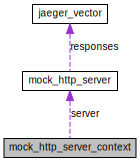
\includegraphics[width=212pt]{structmock__http__server__context__coll__graph}
\end{center}
\end{figure}
\subsection*{Data Fields}
\begin{DoxyCompactItemize}
\item 
\mbox{\Hypertarget{structmock__http__server__context_adef76ed5e4beb0486e1959394916b615}\label{structmock__http__server__context_adef76ed5e4beb0486e1959394916b615}} 
\mbox{\hyperlink{structmock__http__server}{mock\+\_\+http\+\_\+server}} $\ast$ {\bfseries server}
\item 
\mbox{\Hypertarget{structmock__http__server__context_ae4e7c2ec9e13a9aec76bfd78a2e613fc}\label{structmock__http__server__context_ae4e7c2ec9e13a9aec76bfd78a2e613fc}} 
jaeger\+\_\+cond {\bfseries cv}
\end{DoxyCompactItemize}


The documentation for this struct was generated from the following file\+:\begin{DoxyCompactItemize}
\item 
jaegertracingc/\mbox{\hyperlink{mock__agent_8h}{mock\+\_\+agent.\+h}}\end{DoxyCompactItemize}

\hypertarget{structparsing__context}{}\section{parsing\+\_\+context Struct Reference}
\label{structparsing__context}\index{parsing\+\_\+context@{parsing\+\_\+context}}


Collaboration diagram for parsing\+\_\+context\+:\nopagebreak
\begin{figure}[H]
\begin{center}
\leavevmode
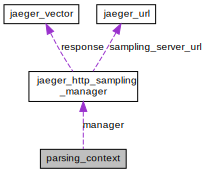
\includegraphics[width=278pt]{structparsing__context__coll__graph}
\end{center}
\end{figure}
\subsection*{Data Fields}
\begin{DoxyCompactItemize}
\item 
\mbox{\Hypertarget{structparsing__context_a9d4da006c6c9f2f167fc788b463965f0}\label{structparsing__context_a9d4da006c6c9f2f167fc788b463965f0}} 
\mbox{\hyperlink{structjaeger__http__sampling__manager}{jaeger\+\_\+http\+\_\+sampling\+\_\+manager}} $\ast$ {\bfseries manager}
\item 
\mbox{\Hypertarget{structparsing__context_a4887f832590917a2b3850dbde0b2946d}\label{structparsing__context_a4887f832590917a2b3850dbde0b2946d}} 
int {\bfseries state}
\end{DoxyCompactItemize}


The documentation for this struct was generated from the following file\+:\begin{DoxyCompactItemize}
\item 
jaegertracingc/sampler.\+c\end{DoxyCompactItemize}

\chapter{File Documentation}
\hypertarget{alloc_8h}{}\section{jaegertracingc/alloc.h File Reference}
\label{alloc_8h}\index{jaegertracingc/alloc.\+h@{jaegertracingc/alloc.\+h}}


Allocator struct and functions.  


{\ttfamily \#include $<$assert.\+h$>$}\newline
{\ttfamily \#include $<$stdint.\+h$>$}\newline
{\ttfamily \#include $<$string.\+h$>$}\newline
{\ttfamily \#include \char`\"{}jaegertracingc/logging.\+h\char`\"{}}\newline
Include dependency graph for alloc.\+h\+:\nopagebreak
\begin{figure}[H]
\begin{center}
\leavevmode
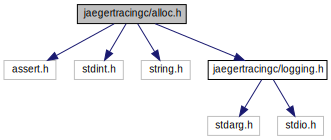
\includegraphics[width=350pt]{alloc_8h__incl}
\end{center}
\end{figure}
This graph shows which files directly or indirectly include this file\+:\nopagebreak
\begin{figure}[H]
\begin{center}
\leavevmode
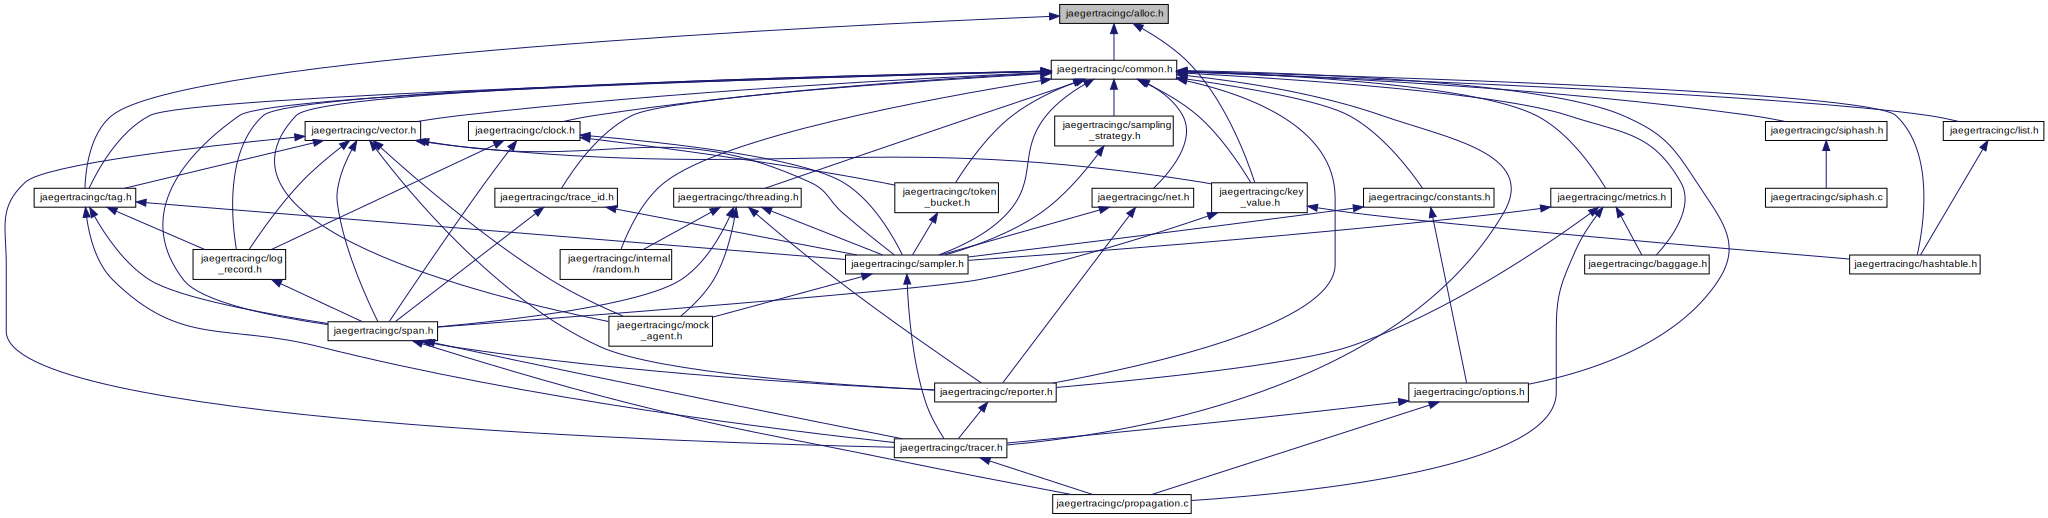
\includegraphics[width=350pt]{alloc_8h__dep__incl}
\end{center}
\end{figure}
\subsection*{Data Structures}
\begin{DoxyCompactItemize}
\item 
struct \mbox{\hyperlink{structjaeger__allocator}{jaeger\+\_\+allocator}}
\begin{DoxyCompactList}\small\item\em Interface to override default allocator. \end{DoxyCompactList}\end{DoxyCompactItemize}
\subsection*{Typedefs}
\begin{DoxyCompactItemize}
\item 
typedef struct \mbox{\hyperlink{structjaeger__allocator}{jaeger\+\_\+allocator}} \mbox{\hyperlink{alloc_8h_a2a438fd982df387349202a40bfca6050}{jaeger\+\_\+allocator}}
\begin{DoxyCompactList}\small\item\em Interface to override default allocator. \end{DoxyCompactList}\end{DoxyCompactItemize}
\subsection*{Functions}
\begin{DoxyCompactItemize}
\item 
\mbox{\hyperlink{structjaeger__allocator}{jaeger\+\_\+allocator}} $\ast$ \mbox{\hyperlink{alloc_8h_abba0f94c3fc30d4184dd15706fff3879}{jaeger\+\_\+built\+\_\+in\+\_\+allocator}} (void)
\begin{DoxyCompactList}\small\item\em Wrapper for built-\/in allocation functions. \end{DoxyCompactList}\item 
\mbox{\hyperlink{structjaeger__allocator}{jaeger\+\_\+allocator}} $\ast$ \mbox{\hyperlink{alloc_8h_a312e479c128951e44cbfeab715691a82}{jaeger\+\_\+null\+\_\+allocator}} (void)
\begin{DoxyCompactList}\small\item\em Wrapper for null allocation functions. \end{DoxyCompactList}\item 
void \mbox{\hyperlink{alloc_8h_a028e4a5c56db3be5bd20496b1a64f920}{jaeger\+\_\+set\+\_\+allocator}} (\mbox{\hyperlink{structjaeger__allocator}{jaeger\+\_\+allocator}} $\ast$alloc)
\begin{DoxyCompactList}\small\item\em Set the installed allocator. \end{DoxyCompactList}\item 
\mbox{\hyperlink{structjaeger__allocator}{jaeger\+\_\+allocator}} $\ast$ \mbox{\hyperlink{alloc_8h_abd1b3422f9bfb294c07bcb44ec2c26e7}{jaeger\+\_\+get\+\_\+allocator}} (void)
\begin{DoxyCompactList}\small\item\em Get the installed allocator. \end{DoxyCompactList}\item 
void $\ast$ \mbox{\hyperlink{alloc_8h_a8bf91f5b7b45e1e602d5a4079420bcd3}{jaeger\+\_\+malloc}} (size\+\_\+t sz)
\begin{DoxyCompactList}\small\item\em Returns result of call to malloc using installed allocator. \end{DoxyCompactList}\item 
void $\ast$ \mbox{\hyperlink{alloc_8h_a2f9fd6513d1b13e8be7d42abf89ad140}{jaeger\+\_\+realloc}} (void $\ast$ptr, size\+\_\+t sz)
\begin{DoxyCompactList}\small\item\em Returns result of call to realloc using installed allocator. \end{DoxyCompactList}\item 
void \mbox{\hyperlink{alloc_8h_ad094b3d57aa0ee6af7b5d3d347a578e5}{jaeger\+\_\+free}} (void $\ast$ptr)
\begin{DoxyCompactList}\small\item\em Calls free using installed allocator. \end{DoxyCompactList}\end{DoxyCompactItemize}


\subsection{Detailed Description}
Allocator struct and functions. 



\subsection{Typedef Documentation}
\mbox{\Hypertarget{alloc_8h_a2a438fd982df387349202a40bfca6050}\label{alloc_8h_a2a438fd982df387349202a40bfca6050}} 
\index{alloc.\+h@{alloc.\+h}!jaeger\+\_\+allocator@{jaeger\+\_\+allocator}}
\index{jaeger\+\_\+allocator@{jaeger\+\_\+allocator}!alloc.\+h@{alloc.\+h}}
\subsubsection{\texorpdfstring{jaeger\+\_\+allocator}{jaeger\_allocator}}
{\footnotesize\ttfamily typedef struct \mbox{\hyperlink{structjaeger__allocator}{jaeger\+\_\+allocator}}  \mbox{\hyperlink{structjaeger__allocator}{jaeger\+\_\+allocator}}}



Interface to override default allocator. 



\subsection{Function Documentation}
\mbox{\Hypertarget{alloc_8h_abba0f94c3fc30d4184dd15706fff3879}\label{alloc_8h_abba0f94c3fc30d4184dd15706fff3879}} 
\index{alloc.\+h@{alloc.\+h}!jaeger\+\_\+built\+\_\+in\+\_\+allocator@{jaeger\+\_\+built\+\_\+in\+\_\+allocator}}
\index{jaeger\+\_\+built\+\_\+in\+\_\+allocator@{jaeger\+\_\+built\+\_\+in\+\_\+allocator}!alloc.\+h@{alloc.\+h}}
\subsubsection{\texorpdfstring{jaeger\+\_\+built\+\_\+in\+\_\+allocator()}{jaeger\_built\_in\_allocator()}}
{\footnotesize\ttfamily \mbox{\hyperlink{structjaeger__allocator}{jaeger\+\_\+allocator}}$\ast$ jaeger\+\_\+built\+\_\+in\+\_\+allocator (\begin{DoxyParamCaption}\item[{void}]{ }\end{DoxyParamCaption})}



Wrapper for built-\/in allocation functions. 

\begin{DoxyReturn}{Returns}
Shared instance of built-\/in allocator. DO N\+OT M\+O\+D\+I\+FY M\+E\+M\+B\+E\+R\+S! 
\end{DoxyReturn}
\mbox{\Hypertarget{alloc_8h_ad094b3d57aa0ee6af7b5d3d347a578e5}\label{alloc_8h_ad094b3d57aa0ee6af7b5d3d347a578e5}} 
\index{alloc.\+h@{alloc.\+h}!jaeger\+\_\+free@{jaeger\+\_\+free}}
\index{jaeger\+\_\+free@{jaeger\+\_\+free}!alloc.\+h@{alloc.\+h}}
\subsubsection{\texorpdfstring{jaeger\+\_\+free()}{jaeger\_free()}}
{\footnotesize\ttfamily void jaeger\+\_\+free (\begin{DoxyParamCaption}\item[{void $\ast$}]{ptr }\end{DoxyParamCaption})}



Calls free using installed allocator. 


\begin{DoxyParams}{Parameters}
{\em ptr} & Allocated address. \\
\hline
\end{DoxyParams}
\mbox{\Hypertarget{alloc_8h_abd1b3422f9bfb294c07bcb44ec2c26e7}\label{alloc_8h_abd1b3422f9bfb294c07bcb44ec2c26e7}} 
\index{alloc.\+h@{alloc.\+h}!jaeger\+\_\+get\+\_\+allocator@{jaeger\+\_\+get\+\_\+allocator}}
\index{jaeger\+\_\+get\+\_\+allocator@{jaeger\+\_\+get\+\_\+allocator}!alloc.\+h@{alloc.\+h}}
\subsubsection{\texorpdfstring{jaeger\+\_\+get\+\_\+allocator()}{jaeger\_get\_allocator()}}
{\footnotesize\ttfamily \mbox{\hyperlink{structjaeger__allocator}{jaeger\+\_\+allocator}}$\ast$ jaeger\+\_\+get\+\_\+allocator (\begin{DoxyParamCaption}\item[{void}]{ }\end{DoxyParamCaption})}



Get the installed allocator. 

\begin{DoxyReturn}{Returns}
alloc Allocator instance. 
\end{DoxyReturn}
\mbox{\Hypertarget{alloc_8h_a8bf91f5b7b45e1e602d5a4079420bcd3}\label{alloc_8h_a8bf91f5b7b45e1e602d5a4079420bcd3}} 
\index{alloc.\+h@{alloc.\+h}!jaeger\+\_\+malloc@{jaeger\+\_\+malloc}}
\index{jaeger\+\_\+malloc@{jaeger\+\_\+malloc}!alloc.\+h@{alloc.\+h}}
\subsubsection{\texorpdfstring{jaeger\+\_\+malloc()}{jaeger\_malloc()}}
{\footnotesize\ttfamily void$\ast$ jaeger\+\_\+malloc (\begin{DoxyParamCaption}\item[{size\+\_\+t}]{sz }\end{DoxyParamCaption})}



Returns result of call to malloc using installed allocator. 


\begin{DoxyParams}{Parameters}
{\em sz} & Size to be allocated. \\
\hline
\end{DoxyParams}
\begin{DoxyReturn}{Returns}
Address to allocated memory on success, N\+U\+LL otherwise. 
\end{DoxyReturn}
\mbox{\Hypertarget{alloc_8h_a312e479c128951e44cbfeab715691a82}\label{alloc_8h_a312e479c128951e44cbfeab715691a82}} 
\index{alloc.\+h@{alloc.\+h}!jaeger\+\_\+null\+\_\+allocator@{jaeger\+\_\+null\+\_\+allocator}}
\index{jaeger\+\_\+null\+\_\+allocator@{jaeger\+\_\+null\+\_\+allocator}!alloc.\+h@{alloc.\+h}}
\subsubsection{\texorpdfstring{jaeger\+\_\+null\+\_\+allocator()}{jaeger\_null\_allocator()}}
{\footnotesize\ttfamily \mbox{\hyperlink{structjaeger__allocator}{jaeger\+\_\+allocator}}$\ast$ jaeger\+\_\+null\+\_\+allocator (\begin{DoxyParamCaption}\item[{void}]{ }\end{DoxyParamCaption})}



Wrapper for null allocation functions. 

Never allocates memory, all function are no-\/ops. Used for testing. \begin{DoxyReturn}{Returns}
Shared instance of null allocator. DO N\+OT M\+O\+D\+I\+FY M\+E\+M\+B\+E\+R\+S! 
\end{DoxyReturn}
\mbox{\Hypertarget{alloc_8h_a2f9fd6513d1b13e8be7d42abf89ad140}\label{alloc_8h_a2f9fd6513d1b13e8be7d42abf89ad140}} 
\index{alloc.\+h@{alloc.\+h}!jaeger\+\_\+realloc@{jaeger\+\_\+realloc}}
\index{jaeger\+\_\+realloc@{jaeger\+\_\+realloc}!alloc.\+h@{alloc.\+h}}
\subsubsection{\texorpdfstring{jaeger\+\_\+realloc()}{jaeger\_realloc()}}
{\footnotesize\ttfamily void$\ast$ jaeger\+\_\+realloc (\begin{DoxyParamCaption}\item[{void $\ast$}]{ptr,  }\item[{size\+\_\+t}]{sz }\end{DoxyParamCaption})}



Returns result of call to realloc using installed allocator. 


\begin{DoxyParams}{Parameters}
{\em ptr} & Pointer to previously allocated memory. \\
\hline
{\em sz} & New size to allocate. \\
\hline
\end{DoxyParams}
\begin{DoxyReturn}{Returns}
Address to allocated memory on success, N\+U\+LL otherwise. 
\end{DoxyReturn}
\mbox{\Hypertarget{alloc_8h_a028e4a5c56db3be5bd20496b1a64f920}\label{alloc_8h_a028e4a5c56db3be5bd20496b1a64f920}} 
\index{alloc.\+h@{alloc.\+h}!jaeger\+\_\+set\+\_\+allocator@{jaeger\+\_\+set\+\_\+allocator}}
\index{jaeger\+\_\+set\+\_\+allocator@{jaeger\+\_\+set\+\_\+allocator}!alloc.\+h@{alloc.\+h}}
\subsubsection{\texorpdfstring{jaeger\+\_\+set\+\_\+allocator()}{jaeger\_set\_allocator()}}
{\footnotesize\ttfamily void jaeger\+\_\+set\+\_\+allocator (\begin{DoxyParamCaption}\item[{\mbox{\hyperlink{structjaeger__allocator}{jaeger\+\_\+allocator}} $\ast$}]{alloc }\end{DoxyParamCaption})}



Set the installed allocator. 


\begin{DoxyParams}{Parameters}
{\em alloc} & Allocator instance. \\
\hline
\end{DoxyParams}

\hypertarget{baggage_8h}{}\section{jaegertracingc/baggage.h File Reference}
\label{baggage_8h}\index{jaegertracingc/baggage.\+h@{jaegertracingc/baggage.\+h}}


Baggage restriction utilities.  


{\ttfamily \#include \char`\"{}jaegertracingc/common.\+h\char`\"{}}\newline
{\ttfamily \#include \char`\"{}jaegertracingc/metrics.\+h\char`\"{}}\newline
{\ttfamily \#include \char`\"{}jaegertracingc/span.\+h\char`\"{}}\newline
Include dependency graph for baggage.\+h\+:
\nopagebreak
\begin{figure}[H]
\begin{center}
\leavevmode
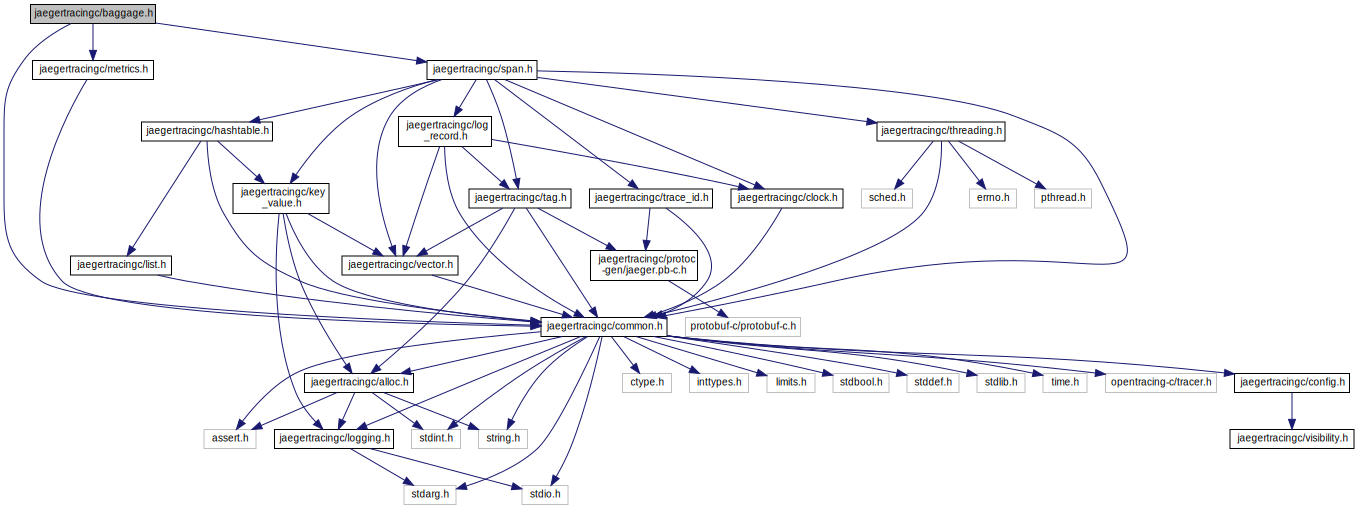
\includegraphics[width=350pt]{baggage_8h__incl}
\end{center}
\end{figure}
\subsection*{Data Structures}
\begin{DoxyCompactItemize}
\item 
struct \mbox{\hyperlink{structjaeger__baggage__restriction}{jaeger\+\_\+baggage\+\_\+restriction}}
\begin{DoxyCompactList}\small\item\em Representation of baggage restriction for a given key and a given service. \end{DoxyCompactList}\item 
struct \mbox{\hyperlink{structjaeger__baggage__restriction__manager}{jaeger\+\_\+baggage\+\_\+restriction\+\_\+manager}}
\begin{DoxyCompactList}\small\item\em Interface for object that manages baggage restrictions. \end{DoxyCompactList}\item 
struct \mbox{\hyperlink{structjaeger__default__baggage__restriction__manager}{jaeger\+\_\+default\+\_\+baggage\+\_\+restriction\+\_\+manager}}
\begin{DoxyCompactList}\small\item\em Default implementation of \mbox{\hyperlink{structjaeger__baggage__restriction__manager}{jaeger\+\_\+baggage\+\_\+restriction\+\_\+manager}} interface. \end{DoxyCompactList}\item 
struct \mbox{\hyperlink{structjaeger__baggage__setter}{jaeger\+\_\+baggage\+\_\+setter}}
\begin{DoxyCompactList}\small\item\em Facade to enforce remote baggage restrictions in tracer. \end{DoxyCompactList}\end{DoxyCompactItemize}
\subsection*{Typedefs}
\begin{DoxyCompactItemize}
\item 
\mbox{\Hypertarget{baggage_8h_ada4c9c7abbbd019adc8cb34ac7c9fbb1}\label{baggage_8h_ada4c9c7abbbd019adc8cb34ac7c9fbb1}} 
typedef struct \mbox{\hyperlink{structjaeger__baggage__restriction}{jaeger\+\_\+baggage\+\_\+restriction}} \mbox{\hyperlink{baggage_8h_ada4c9c7abbbd019adc8cb34ac7c9fbb1}{jaeger\+\_\+baggage\+\_\+restriction}}
\begin{DoxyCompactList}\small\item\em Representation of baggage restriction for a given key and a given service. \end{DoxyCompactList}\item 
\mbox{\Hypertarget{baggage_8h_a9a046fcbddca1d9350b8783fa8a7b6b9}\label{baggage_8h_a9a046fcbddca1d9350b8783fa8a7b6b9}} 
typedef struct \mbox{\hyperlink{structjaeger__baggage__restriction__manager}{jaeger\+\_\+baggage\+\_\+restriction\+\_\+manager}} \mbox{\hyperlink{baggage_8h_a9a046fcbddca1d9350b8783fa8a7b6b9}{jaeger\+\_\+baggage\+\_\+restriction\+\_\+manager}}
\begin{DoxyCompactList}\small\item\em Interface for object that manages baggage restrictions. \end{DoxyCompactList}\item 
\mbox{\Hypertarget{baggage_8h_a7b7fa3edf0965250a6fed48c98edce0e}\label{baggage_8h_a7b7fa3edf0965250a6fed48c98edce0e}} 
typedef struct \mbox{\hyperlink{structjaeger__default__baggage__restriction__manager}{jaeger\+\_\+default\+\_\+baggage\+\_\+restriction\+\_\+manager}} \mbox{\hyperlink{baggage_8h_a7b7fa3edf0965250a6fed48c98edce0e}{jaeger\+\_\+default\+\_\+baggage\+\_\+restriction\+\_\+manager}}
\begin{DoxyCompactList}\small\item\em Default implementation of \mbox{\hyperlink{structjaeger__baggage__restriction__manager}{jaeger\+\_\+baggage\+\_\+restriction\+\_\+manager}} interface. \end{DoxyCompactList}\item 
typedef struct \mbox{\hyperlink{structjaeger__baggage__setter}{jaeger\+\_\+baggage\+\_\+setter}} \mbox{\hyperlink{baggage_8h_a63a49536e4600e077a0e684d79a57706}{jaeger\+\_\+baggage\+\_\+setter}}
\begin{DoxyCompactList}\small\item\em Facade to enforce remote baggage restrictions in tracer. \end{DoxyCompactList}\end{DoxyCompactItemize}
\subsection*{Functions}
\begin{DoxyCompactItemize}
\item 
\mbox{\Hypertarget{baggage_8h_aea3ddc7284cebc6d4979b628d59f54bd}\label{baggage_8h_aea3ddc7284cebc6d4979b628d59f54bd}} 
void {\bfseries jaeger\+\_\+baggage\+\_\+setter\+\_\+set\+\_\+baggage} (\mbox{\hyperlink{structjaeger__baggage__setter}{jaeger\+\_\+baggage\+\_\+setter}} $\ast$setter, \mbox{\hyperlink{structjaeger__span}{jaeger\+\_\+span}} $\ast$span, const char $\ast$key, const char $\ast$value)
\end{DoxyCompactItemize}


\subsection{Detailed Description}
Baggage restriction utilities. 



\subsection{Typedef Documentation}
\mbox{\Hypertarget{baggage_8h_a63a49536e4600e077a0e684d79a57706}\label{baggage_8h_a63a49536e4600e077a0e684d79a57706}} 
\index{baggage.\+h@{baggage.\+h}!jaeger\+\_\+baggage\+\_\+setter@{jaeger\+\_\+baggage\+\_\+setter}}
\index{jaeger\+\_\+baggage\+\_\+setter@{jaeger\+\_\+baggage\+\_\+setter}!baggage.\+h@{baggage.\+h}}
\subsubsection{\texorpdfstring{jaeger\+\_\+baggage\+\_\+setter}{jaeger\_baggage\_setter}}
{\footnotesize\ttfamily typedef struct \mbox{\hyperlink{structjaeger__baggage__setter}{jaeger\+\_\+baggage\+\_\+setter}}  \mbox{\hyperlink{structjaeger__baggage__setter}{jaeger\+\_\+baggage\+\_\+setter}}}



Facade to enforce remote baggage restrictions in tracer. 


\hypertarget{clock_8h}{}\section{jaegertracingc/clock.h File Reference}
\label{clock_8h}\index{jaegertracingc/clock.\+h@{jaegertracingc/clock.\+h}}


Timestamp and duration representations.  


{\ttfamily \#include \char`\"{}jaegertracingc/common.\+h\char`\"{}}\newline
Include dependency graph for clock.\+h\+:\nopagebreak
\begin{figure}[H]
\begin{center}
\leavevmode
\includegraphics[width=350pt]{clock_8h__incl}
\end{center}
\end{figure}
This graph shows which files directly or indirectly include this file\+:\nopagebreak
\begin{figure}[H]
\begin{center}
\leavevmode
\includegraphics[width=350pt]{clock_8h__dep__incl}
\end{center}
\end{figure}
\subsection*{Macros}
\begin{DoxyCompactItemize}
\item 
\mbox{\Hypertarget{clock_8h_a2063a571cd76bc80e468c7eb7acd4948}\label{clock_8h_a2063a571cd76bc80e468c7eb7acd4948}} 
\#define {\bfseries J\+A\+E\+G\+E\+R\+T\+R\+A\+C\+I\+N\+G\+C\+\_\+\+N\+A\+N\+O\+S\+E\+C\+O\+N\+D\+S\+\_\+\+P\+E\+R\+\_\+\+S\+E\+C\+O\+ND}~1000000000
\item 
\mbox{\Hypertarget{clock_8h_a2d254e2e8e84115eae0bb9ea37958e8f}\label{clock_8h_a2d254e2e8e84115eae0bb9ea37958e8f}} 
\#define {\bfseries J\+A\+E\+G\+E\+R\+T\+R\+A\+C\+I\+N\+G\+C\+\_\+\+M\+I\+C\+R\+O\+S\+E\+C\+O\+N\+D\+S\+\_\+\+P\+E\+R\+\_\+\+S\+E\+C\+O\+ND}~1000000
\item 
\mbox{\Hypertarget{clock_8h_a2b2d7ecbc3f251c08dc350dd34a49c79}\label{clock_8h_a2b2d7ecbc3f251c08dc350dd34a49c79}} 
\#define {\bfseries J\+A\+E\+G\+E\+R\+T\+R\+A\+C\+I\+N\+G\+C\+\_\+\+N\+A\+N\+O\+S\+E\+C\+O\+N\+D\+S\+\_\+\+P\+E\+R\+\_\+\+M\+I\+C\+R\+O\+S\+E\+C\+O\+ND}~1000
\item 
\#define {\bfseries J\+A\+E\+G\+E\+R\+T\+R\+A\+C\+I\+N\+G\+C\+\_\+\+T\+I\+M\+E\+\_\+\+C\+A\+ST}(x,  type)
\item 
\#define {\bfseries J\+A\+E\+G\+E\+R\+T\+R\+A\+C\+I\+N\+G\+C\+\_\+\+T\+I\+M\+E\+S\+T\+A\+M\+P\+\_\+\+I\+N\+IT}
\item 
\mbox{\Hypertarget{clock_8h_a8b5b653bbbf733c984d505c29f95ebe8}\label{clock_8h_a8b5b653bbbf733c984d505c29f95ebe8}} 
\#define {\bfseries J\+A\+E\+G\+E\+R\+T\+R\+A\+C\+I\+N\+G\+C\+\_\+\+D\+U\+R\+A\+T\+I\+O\+N\+\_\+\+I\+N\+IT}~J\+A\+E\+G\+E\+R\+T\+R\+A\+C\+I\+N\+G\+C\+\_\+\+T\+I\+M\+E\+S\+T\+A\+M\+P\+\_\+\+I\+N\+IT
\end{DoxyCompactItemize}
\subsection*{Typedefs}
\begin{DoxyCompactItemize}
\item 
\mbox{\Hypertarget{clock_8h_ab709536a0ff5199c2e1e364a79ae9808}\label{clock_8h_ab709536a0ff5199c2e1e364a79ae9808}} 
typedef opentracing\+\_\+duration {\bfseries jaeger\+\_\+duration}
\item 
\mbox{\Hypertarget{clock_8h_a3d95f77c13cc89c2a8c3e10f6c9b154f}\label{clock_8h_a3d95f77c13cc89c2a8c3e10f6c9b154f}} 
typedef opentracing\+\_\+timestamp {\bfseries jaeger\+\_\+timestamp}
\end{DoxyCompactItemize}


\subsection{Detailed Description}
Timestamp and duration representations. 



\subsection{Macro Definition Documentation}
\mbox{\Hypertarget{clock_8h_a937506357c9229e7492b7126313364c0}\label{clock_8h_a937506357c9229e7492b7126313364c0}} 
\index{clock.\+h@{clock.\+h}!J\+A\+E\+G\+E\+R\+T\+R\+A\+C\+I\+N\+G\+C\+\_\+\+T\+I\+M\+E\+\_\+\+C\+A\+ST@{J\+A\+E\+G\+E\+R\+T\+R\+A\+C\+I\+N\+G\+C\+\_\+\+T\+I\+M\+E\+\_\+\+C\+A\+ST}}
\index{J\+A\+E\+G\+E\+R\+T\+R\+A\+C\+I\+N\+G\+C\+\_\+\+T\+I\+M\+E\+\_\+\+C\+A\+ST@{J\+A\+E\+G\+E\+R\+T\+R\+A\+C\+I\+N\+G\+C\+\_\+\+T\+I\+M\+E\+\_\+\+C\+A\+ST}!clock.\+h@{clock.\+h}}
\subsubsection{\texorpdfstring{J\+A\+E\+G\+E\+R\+T\+R\+A\+C\+I\+N\+G\+C\+\_\+\+T\+I\+M\+E\+\_\+\+C\+A\+ST}{JAEGERTRACINGC\_TIME\_CAST}}
{\footnotesize\ttfamily \#define J\+A\+E\+G\+E\+R\+T\+R\+A\+C\+I\+N\+G\+C\+\_\+\+T\+I\+M\+E\+\_\+\+C\+A\+ST(\begin{DoxyParamCaption}\item[{}]{x,  }\item[{}]{type }\end{DoxyParamCaption})}

{\bfseries Value\+:}
\begin{DoxyCode}
\DoxyCodeLine{(type)                                           \(\backslash\)}
\DoxyCodeLine{    \{                                                \(\backslash\)}
\DoxyCodeLine{        .tv\_sec = (x).tv\_sec, .tv\_nsec = (x).tv\_nsec \(\backslash\)}
\DoxyCodeLine{    \}}
\end{DoxyCode}
\mbox{\Hypertarget{clock_8h_adeef897ea2f31d9b82a5f512d25f00b2}\label{clock_8h_adeef897ea2f31d9b82a5f512d25f00b2}} 
\index{clock.\+h@{clock.\+h}!J\+A\+E\+G\+E\+R\+T\+R\+A\+C\+I\+N\+G\+C\+\_\+\+T\+I\+M\+E\+S\+T\+A\+M\+P\+\_\+\+I\+N\+IT@{J\+A\+E\+G\+E\+R\+T\+R\+A\+C\+I\+N\+G\+C\+\_\+\+T\+I\+M\+E\+S\+T\+A\+M\+P\+\_\+\+I\+N\+IT}}
\index{J\+A\+E\+G\+E\+R\+T\+R\+A\+C\+I\+N\+G\+C\+\_\+\+T\+I\+M\+E\+S\+T\+A\+M\+P\+\_\+\+I\+N\+IT@{J\+A\+E\+G\+E\+R\+T\+R\+A\+C\+I\+N\+G\+C\+\_\+\+T\+I\+M\+E\+S\+T\+A\+M\+P\+\_\+\+I\+N\+IT}!clock.\+h@{clock.\+h}}
\subsubsection{\texorpdfstring{J\+A\+E\+G\+E\+R\+T\+R\+A\+C\+I\+N\+G\+C\+\_\+\+T\+I\+M\+E\+S\+T\+A\+M\+P\+\_\+\+I\+N\+IT}{JAEGERTRACINGC\_TIMESTAMP\_INIT}}
{\footnotesize\ttfamily \#define J\+A\+E\+G\+E\+R\+T\+R\+A\+C\+I\+N\+G\+C\+\_\+\+T\+I\+M\+E\+S\+T\+A\+M\+P\+\_\+\+I\+N\+IT}

{\bfseries Value\+:}
\begin{DoxyCode}
\DoxyCodeLine{\{                                         \(\backslash\)}
\DoxyCodeLine{        .value = \{.tv\_sec = 0, .tv\_nsec = 0 \} \(\backslash\)}
\DoxyCodeLine{    \}}
\end{DoxyCode}

\hypertarget{common_8h}{}\section{jaegertracingc/common.h File Reference}
\label{common_8h}\index{jaegertracingc/common.\+h@{jaegertracingc/common.\+h}}


Common headers, struct definitions, and macros.  


{\ttfamily \#include \char`\"{}jaegertracingc/config.\+h\char`\"{}}\newline
{\ttfamily \#include $<$assert.\+h$>$}\newline
{\ttfamily \#include $<$ctype.\+h$>$}\newline
{\ttfamily \#include $<$inttypes.\+h$>$}\newline
{\ttfamily \#include $<$limits.\+h$>$}\newline
{\ttfamily \#include $<$stdarg.\+h$>$}\newline
{\ttfamily \#include $<$stdbool.\+h$>$}\newline
{\ttfamily \#include $<$stddef.\+h$>$}\newline
{\ttfamily \#include $<$stdint.\+h$>$}\newline
{\ttfamily \#include $<$stdio.\+h$>$}\newline
{\ttfamily \#include $<$stdlib.\+h$>$}\newline
{\ttfamily \#include $<$string.\+h$>$}\newline
{\ttfamily \#include $<$time.\+h$>$}\newline
{\ttfamily \#include $<$opentracing-\/c/tracer.\+h$>$}\newline
{\ttfamily \#include \char`\"{}jaegertracingc/alloc.\+h\char`\"{}}\newline
{\ttfamily \#include \char`\"{}jaegertracingc/logging.\+h\char`\"{}}\newline
Include dependency graph for common.\+h\+:\nopagebreak
\begin{figure}[H]
\begin{center}
\leavevmode
\includegraphics[width=350pt]{common_8h__incl}
\end{center}
\end{figure}
This graph shows which files directly or indirectly include this file\+:\nopagebreak
\begin{figure}[H]
\begin{center}
\leavevmode
\includegraphics[width=350pt]{common_8h__dep__incl}
\end{center}
\end{figure}
\subsection*{Macros}
\begin{DoxyCompactItemize}
\item 
\mbox{\Hypertarget{common_8h_a13c0d0867a4b947c42da396748a5904c}\label{common_8h_a13c0d0867a4b947c42da396748a5904c}} 
\#define {\bfseries J\+A\+E\+G\+E\+R\+T\+R\+A\+C\+I\+N\+G\+C\+\_\+\+M\+IN}(a,  b)~((b) $<$ (a) ? (b) \+: (a))
\item 
\mbox{\Hypertarget{common_8h_ac7c1ab8a78f50c841ce04e6ad138bb39}\label{common_8h_ac7c1ab8a78f50c841ce04e6ad138bb39}} 
\#define {\bfseries J\+A\+E\+G\+E\+R\+T\+R\+A\+C\+I\+N\+G\+C\+\_\+\+M\+AX}(a,  b)~((b) $>$ (a) ? (b) \+: (a))
\item 
\mbox{\Hypertarget{common_8h_a16a48930251e58744abe552322bf429a}\label{common_8h_a16a48930251e58744abe552322bf429a}} 
\#define {\bfseries J\+A\+E\+G\+E\+R\+T\+R\+A\+C\+I\+N\+G\+C\+\_\+\+C\+L\+A\+MP}(x,  low,  high)~J\+A\+E\+G\+E\+R\+T\+R\+A\+C\+I\+N\+G\+C\+\_\+\+M\+IN(J\+A\+E\+G\+E\+R\+T\+R\+A\+C\+I\+N\+G\+C\+\_\+\+M\+AX((x), (low)), (high))
\item 
\mbox{\Hypertarget{common_8h_ae739cfd0f1af79e3e53d62aff875eaae}\label{common_8h_ae739cfd0f1af79e3e53d62aff875eaae}} 
\#define {\bfseries J\+A\+E\+G\+E\+R\+T\+R\+A\+C\+I\+N\+G\+C\+\_\+\+C\+O\+N\+T\+A\+I\+N\+E\+R\+\_\+\+OF}(ptr,  type,  member)~(type$\ast$) (((char$\ast$) (ptr)) -\/ offsetof(type, member))
\end{DoxyCompactItemize}
\subsection*{Typedefs}
\begin{DoxyCompactItemize}
\item 
\mbox{\Hypertarget{common_8h_ac181b00dbfc4357a9b4e2c5908a8a425}\label{common_8h_ac181b00dbfc4357a9b4e2c5908a8a425}} 
typedef opentracing\+\_\+destructible {\bfseries jaeger\+\_\+destructible}
\end{DoxyCompactItemize}


\subsection{Detailed Description}
Common headers, struct definitions, and macros. 


\hypertarget{hashtable_8h}{}\section{jaegertracingc/hashtable.h File Reference}
\label{hashtable_8h}\index{jaegertracingc/hashtable.\+h@{jaegertracingc/hashtable.\+h}}


Hashtable data structure.  


{\ttfamily \#include \char`\"{}jaegertracingc/common.\+h\char`\"{}}\newline
{\ttfamily \#include \char`\"{}jaegertracingc/key\+\_\+value.\+h\char`\"{}}\newline
{\ttfamily \#include \char`\"{}jaegertracingc/list.\+h\char`\"{}}\newline
Include dependency graph for hashtable.\+h\+:\nopagebreak
\begin{figure}[H]
\begin{center}
\leavevmode
\includegraphics[width=350pt]{hashtable_8h__incl}
\end{center}
\end{figure}
This graph shows which files directly or indirectly include this file\+:\nopagebreak
\begin{figure}[H]
\begin{center}
\leavevmode
\includegraphics[width=350pt]{hashtable_8h__dep__incl}
\end{center}
\end{figure}
\subsection*{Data Structures}
\begin{DoxyCompactItemize}
\item 
struct \mbox{\hyperlink{structjaeger__hashtable}{jaeger\+\_\+hashtable}}
\begin{DoxyCompactList}\small\item\em Hashtable data structure. \end{DoxyCompactList}\item 
struct \mbox{\hyperlink{structjaeger__key__value__node}{jaeger\+\_\+key\+\_\+value\+\_\+node}}
\begin{DoxyCompactList}\small\item\em Define link list node for key-\/value pairs. \end{DoxyCompactList}\item 
struct \mbox{\hyperlink{structjaeger__hashtable__lookup__result}{jaeger\+\_\+hashtable\+\_\+lookup\+\_\+result}}
\end{DoxyCompactItemize}
\subsection*{Macros}
\begin{DoxyCompactItemize}
\item 
\mbox{\Hypertarget{hashtable_8h_a6153a13e003c25cfdf828cc58413b377}\label{hashtable_8h_a6153a13e003c25cfdf828cc58413b377}} 
\#define \mbox{\hyperlink{hashtable_8h_a6153a13e003c25cfdf828cc58413b377}{J\+A\+E\+G\+E\+R\+T\+R\+A\+C\+I\+N\+G\+C\+\_\+\+H\+A\+S\+H\+T\+A\+B\+L\+E\+\_\+\+I\+N\+I\+T\+\_\+\+O\+R\+D\+ER}}~4u
\begin{DoxyCompactList}\small\item\em Initial order of new hashtable. \end{DoxyCompactList}\item 
\mbox{\Hypertarget{hashtable_8h_aa201d83aa9bd09cdc682c6ba45e7522e}\label{hashtable_8h_aa201d83aa9bd09cdc682c6ba45e7522e}} 
\#define \mbox{\hyperlink{hashtable_8h_aa201d83aa9bd09cdc682c6ba45e7522e}{J\+A\+E\+G\+E\+R\+T\+R\+A\+C\+I\+N\+G\+C\+\_\+\+H\+A\+S\+H\+T\+A\+B\+L\+E\+\_\+\+T\+H\+R\+E\+S\+H\+O\+LD}}~1.\+0
\begin{DoxyCompactList}\small\item\em Threshold of size to bucket count ratio at which point the hashtable will rehash into a larger table. \end{DoxyCompactList}\item 
\#define \mbox{\hyperlink{hashtable_8h_a3763844cae3e82e4d62724f06d84699a}{J\+A\+E\+G\+E\+R\+T\+R\+A\+C\+I\+N\+G\+C\+\_\+\+H\+A\+S\+H\+T\+A\+B\+L\+E\+\_\+\+I\+N\+IT}}
\begin{DoxyCompactList}\small\item\em Static initializer for hashtable. \end{DoxyCompactList}\end{DoxyCompactItemize}
\subsection*{Typedefs}
\begin{DoxyCompactItemize}
\item 
\mbox{\Hypertarget{hashtable_8h_aa3b27c1f551b5b7027567043389c2c27}\label{hashtable_8h_aa3b27c1f551b5b7027567043389c2c27}} 
typedef struct \mbox{\hyperlink{structjaeger__hashtable}{jaeger\+\_\+hashtable}} \mbox{\hyperlink{hashtable_8h_aa3b27c1f551b5b7027567043389c2c27}{jaeger\+\_\+hashtable}}
\begin{DoxyCompactList}\small\item\em Hashtable data structure. \end{DoxyCompactList}\item 
typedef struct \mbox{\hyperlink{structjaeger__key__value__node}{jaeger\+\_\+key\+\_\+value\+\_\+node}} \mbox{\hyperlink{hashtable_8h_a5c403e8fe72ed0ed67b77a4cae29cfd1}{jaeger\+\_\+key\+\_\+value\+\_\+node}}
\begin{DoxyCompactList}\small\item\em Define link list node for key-\/value pairs. \end{DoxyCompactList}\item 
\mbox{\Hypertarget{hashtable_8h_acc18a8c1466117cb5f17e0bb4a040ff3}\label{hashtable_8h_acc18a8c1466117cb5f17e0bb4a040ff3}} 
typedef struct \mbox{\hyperlink{structjaeger__hashtable__lookup__result}{jaeger\+\_\+hashtable\+\_\+lookup\+\_\+result}} {\bfseries jaeger\+\_\+hashtable\+\_\+lookup\+\_\+result}
\end{DoxyCompactItemize}
\subsection*{Functions}
\begin{DoxyCompactItemize}
\item 
\mbox{\Hypertarget{hashtable_8h_ac6818f125682681819bf6cc762293198}\label{hashtable_8h_ac6818f125682681819bf6cc762293198}} 
size\+\_\+t {\bfseries jaeger\+\_\+hashtable\+\_\+hash} (const char $\ast$key)
\item 
\mbox{\Hypertarget{hashtable_8h_a75a51e612240ea78e5ec6a7060233019}\label{hashtable_8h_a75a51e612240ea78e5ec6a7060233019}} 
uint32\+\_\+t {\bfseries jaeger\+\_\+hashtable\+\_\+minimal\+\_\+order} (uint32\+\_\+t size)
\end{DoxyCompactItemize}


\subsection{Detailed Description}
Hashtable data structure. 



\subsection{Macro Definition Documentation}
\mbox{\Hypertarget{hashtable_8h_a3763844cae3e82e4d62724f06d84699a}\label{hashtable_8h_a3763844cae3e82e4d62724f06d84699a}} 
\index{hashtable.\+h@{hashtable.\+h}!J\+A\+E\+G\+E\+R\+T\+R\+A\+C\+I\+N\+G\+C\+\_\+\+H\+A\+S\+H\+T\+A\+B\+L\+E\+\_\+\+I\+N\+IT@{J\+A\+E\+G\+E\+R\+T\+R\+A\+C\+I\+N\+G\+C\+\_\+\+H\+A\+S\+H\+T\+A\+B\+L\+E\+\_\+\+I\+N\+IT}}
\index{J\+A\+E\+G\+E\+R\+T\+R\+A\+C\+I\+N\+G\+C\+\_\+\+H\+A\+S\+H\+T\+A\+B\+L\+E\+\_\+\+I\+N\+IT@{J\+A\+E\+G\+E\+R\+T\+R\+A\+C\+I\+N\+G\+C\+\_\+\+H\+A\+S\+H\+T\+A\+B\+L\+E\+\_\+\+I\+N\+IT}!hashtable.\+h@{hashtable.\+h}}
\subsubsection{\texorpdfstring{J\+A\+E\+G\+E\+R\+T\+R\+A\+C\+I\+N\+G\+C\+\_\+\+H\+A\+S\+H\+T\+A\+B\+L\+E\+\_\+\+I\+N\+IT}{JAEGERTRACINGC\_HASHTABLE\_INIT}}
{\footnotesize\ttfamily \#define J\+A\+E\+G\+E\+R\+T\+R\+A\+C\+I\+N\+G\+C\+\_\+\+H\+A\+S\+H\+T\+A\+B\+L\+E\+\_\+\+I\+N\+IT}

{\bfseries Value\+:}
\begin{DoxyCode}
\DoxyCodeLine{\{                                          \(\backslash\)}
\DoxyCodeLine{        .size = 0, .order = 0, .buckets = NULL \(\backslash\)}
\DoxyCodeLine{    \}}
\end{DoxyCode}


Static initializer for hashtable. 



\subsection{Typedef Documentation}
\mbox{\Hypertarget{hashtable_8h_a5c403e8fe72ed0ed67b77a4cae29cfd1}\label{hashtable_8h_a5c403e8fe72ed0ed67b77a4cae29cfd1}} 
\index{hashtable.\+h@{hashtable.\+h}!jaeger\+\_\+key\+\_\+value\+\_\+node@{jaeger\+\_\+key\+\_\+value\+\_\+node}}
\index{jaeger\+\_\+key\+\_\+value\+\_\+node@{jaeger\+\_\+key\+\_\+value\+\_\+node}!hashtable.\+h@{hashtable.\+h}}
\subsubsection{\texorpdfstring{jaeger\+\_\+key\+\_\+value\+\_\+node}{jaeger\_key\_value\_node}}
{\footnotesize\ttfamily typedef struct \mbox{\hyperlink{structjaeger__key__value__node}{jaeger\+\_\+key\+\_\+value\+\_\+node}}  \mbox{\hyperlink{structjaeger__key__value__node}{jaeger\+\_\+key\+\_\+value\+\_\+node}}}



Define link list node for key-\/value pairs. 


\hypertarget{endian_8h}{}\section{jaegertracingc/internal/endian.h File Reference}
\label{endian_8h}\index{jaegertracingc/internal/endian.\+h@{jaegertracingc/internal/endian.\+h}}
{\ttfamily \#include $<$endian.\+h$>$}\newline
Include dependency graph for endian.\+h\+:\nopagebreak
\begin{figure}[H]
\begin{center}
\leavevmode
\includegraphics[width=210pt]{endian_8h__incl}
\end{center}
\end{figure}
This graph shows which files directly or indirectly include this file\+:\nopagebreak
\begin{figure}[H]
\begin{center}
\leavevmode
\includegraphics[width=224pt]{endian_8h__dep__incl}
\end{center}
\end{figure}
\subsection*{Macros}
\begin{DoxyCompactItemize}
\item 
\mbox{\Hypertarget{endian_8h_ab2d851980460d74a294c99768e68f45c}\label{endian_8h_ab2d851980460d74a294c99768e68f45c}} 
\#define {\bfseries B\+Y\+T\+E\+S\+W\+A\+P64}(x)~be64toh((x))
\item 
\mbox{\Hypertarget{endian_8h_ab55feb41f784e836c8af8902e80e6e04}\label{endian_8h_ab55feb41f784e836c8af8902e80e6e04}} 
\#define {\bfseries B\+Y\+T\+E\+S\+W\+A\+P32}(x)~be32toh((x))
\item 
\mbox{\Hypertarget{endian_8h_a758da2f6ffbe5137c3299ee64e4e9ade}\label{endian_8h_a758da2f6ffbe5137c3299ee64e4e9ade}} 
\#define {\bfseries B\+I\+G\+\_\+\+E\+N\+D\+I\+A\+N\+\_\+64\+\_\+\+T\+O\+\_\+\+H\+O\+ST}(x)~B\+Y\+T\+E\+S\+W\+A\+P64(x)
\item 
\mbox{\Hypertarget{endian_8h_aa7291a2e9ea1417cc2267d7674c81565}\label{endian_8h_aa7291a2e9ea1417cc2267d7674c81565}} 
\#define {\bfseries B\+I\+G\+\_\+\+E\+N\+D\+I\+A\+N\+\_\+32\+\_\+\+T\+O\+\_\+\+H\+O\+ST}(x)~B\+Y\+T\+E\+S\+W\+A\+P32(x)
\item 
\mbox{\Hypertarget{endian_8h_a67fee3084ff2a6a661779b2172d634b4}\label{endian_8h_a67fee3084ff2a6a661779b2172d634b4}} 
\#define {\bfseries H\+O\+S\+T\+\_\+\+T\+O\+\_\+\+B\+I\+G\+\_\+\+E\+N\+D\+I\+A\+N\+\_\+64}(x)~B\+I\+G\+\_\+\+E\+N\+D\+I\+A\+N\+\_\+64\+\_\+\+T\+O\+\_\+\+H\+O\+ST(x)
\item 
\mbox{\Hypertarget{endian_8h_af9e6097802072cead05ad7ce64d38f4d}\label{endian_8h_af9e6097802072cead05ad7ce64d38f4d}} 
\#define {\bfseries H\+O\+S\+T\+\_\+\+T\+O\+\_\+\+B\+I\+G\+\_\+\+E\+N\+D\+I\+A\+N\+\_\+32}(x)~B\+I\+G\+\_\+\+E\+N\+D\+I\+A\+N\+\_\+32\+\_\+\+T\+O\+\_\+\+H\+O\+ST(x)
\end{DoxyCompactItemize}

\hypertarget{random_8h}{}\section{jaegertracingc/random.h File Reference}
\label{random_8h}\index{jaegertracingc/random.\+h@{jaegertracingc/random.\+h}}


Random number generation.  


{\ttfamily \#include $<$stdint.\+h$>$}\newline
Include dependency graph for random.\+h\+:\nopagebreak
\begin{figure}[H]
\begin{center}
\leavevmode
\includegraphics[width=201pt]{random_8h__incl}
\end{center}
\end{figure}
This graph shows which files directly or indirectly include this file\+:\nopagebreak
\begin{figure}[H]
\begin{center}
\leavevmode
\includegraphics[width=201pt]{random_8h__dep__incl}
\end{center}
\end{figure}
\subsection*{Functions}
\begin{DoxyCompactItemize}
\item 
\mbox{\Hypertarget{random_8h_a107727bd7a5be6795b1fb7922a382f43}\label{random_8h_a107727bd7a5be6795b1fb7922a382f43}} 
int64\+\_\+t {\bfseries jaeger\+\_\+random64} (void)
\end{DoxyCompactItemize}


\subsection{Detailed Description}
Random number generation. 


\hypertarget{strings_8h}{}\section{jaegertracingc/internal/strings.h File Reference}
\label{strings_8h}\index{jaegertracingc/internal/strings.\+h@{jaegertracingc/internal/strings.\+h}}
{\ttfamily \#include $<$assert.\+h$>$}\newline
{\ttfamily \#include $<$ctype.\+h$>$}\newline
{\ttfamily \#include $<$string.\+h$>$}\newline
{\ttfamily \#include \char`\"{}jaegertracingc/hashtable.\+h\char`\"{}}\newline
Include dependency graph for strings.\+h\+:\nopagebreak
\begin{figure}[H]
\begin{center}
\leavevmode
\includegraphics[width=350pt]{strings_8h__incl}
\end{center}
\end{figure}
This graph shows which files directly or indirectly include this file\+:\nopagebreak
\begin{figure}[H]
\begin{center}
\leavevmode
\includegraphics[width=219pt]{strings_8h__dep__incl}
\end{center}
\end{figure}
\subsection*{Macros}
\begin{DoxyCompactItemize}
\item 
\#define {\bfseries A\+P\+P\+E\+N\+D\+\_\+\+C\+H\+AR}(x)
\end{DoxyCompactItemize}


\subsection{Macro Definition Documentation}
\mbox{\Hypertarget{strings_8h_a23051ff9579890c9f6df36a71a71277c}\label{strings_8h_a23051ff9579890c9f6df36a71a71277c}} 
\index{strings.\+h@{strings.\+h}!A\+P\+P\+E\+N\+D\+\_\+\+C\+H\+AR@{A\+P\+P\+E\+N\+D\+\_\+\+C\+H\+AR}}
\index{A\+P\+P\+E\+N\+D\+\_\+\+C\+H\+AR@{A\+P\+P\+E\+N\+D\+\_\+\+C\+H\+AR}!strings.\+h@{strings.\+h}}
\subsubsection{\texorpdfstring{A\+P\+P\+E\+N\+D\+\_\+\+C\+H\+AR}{APPEND\_CHAR}}
{\footnotesize\ttfamily \#define A\+P\+P\+E\+N\+D\+\_\+\+C\+H\+AR(\begin{DoxyParamCaption}\item[{}]{x }\end{DoxyParamCaption})}

{\bfseries Value\+:}
\begin{DoxyCode}
\DoxyCodeLine{\textcolor{keywordflow}{do} \{                                    \(\backslash\)}
\DoxyCodeLine{        assert(dst\_len + 1 <= src\_len + 1); \(\backslash\)}
\DoxyCodeLine{        assert((x) < 0x7f);                 \(\backslash\)}
\DoxyCodeLine{        dst[dst\_len] = (x);                 \(\backslash\)}
\DoxyCodeLine{        dst\_len++;                          \(\backslash\)}
\DoxyCodeLine{    \} \textcolor{keywordflow}{while} (0)}
\end{DoxyCode}

\hypertarget{key__value_8h}{}\section{jaegertracingc/key\+\_\+value.h File Reference}
\label{key__value_8h}\index{jaegertracingc/key\+\_\+value.\+h@{jaegertracingc/key\+\_\+value.\+h}}


Key value pair representation.  


{\ttfamily \#include \char`\"{}jaegertracingc/alloc.\+h\char`\"{}}\newline
{\ttfamily \#include \char`\"{}jaegertracingc/common.\+h\char`\"{}}\newline
{\ttfamily \#include \char`\"{}jaegertracingc/logging.\+h\char`\"{}}\newline
{\ttfamily \#include \char`\"{}jaegertracingc/vector.\+h\char`\"{}}\newline
Include dependency graph for key\+\_\+value.\+h\+:\nopagebreak
\begin{figure}[H]
\begin{center}
\leavevmode
\includegraphics[width=350pt]{key__value_8h__incl}
\end{center}
\end{figure}
This graph shows which files directly or indirectly include this file\+:\nopagebreak
\begin{figure}[H]
\begin{center}
\leavevmode
\includegraphics[width=350pt]{key__value_8h__dep__incl}
\end{center}
\end{figure}
\subsection*{Data Structures}
\begin{DoxyCompactItemize}
\item 
struct \mbox{\hyperlink{structjaeger__key__value}{jaeger\+\_\+key\+\_\+value}}
\end{DoxyCompactItemize}
\subsection*{Macros}
\begin{DoxyCompactItemize}
\item 
\#define {\bfseries J\+A\+E\+G\+E\+R\+T\+R\+A\+C\+I\+N\+G\+C\+\_\+\+K\+E\+Y\+\_\+\+V\+A\+L\+U\+E\+\_\+\+I\+N\+IT}
\end{DoxyCompactItemize}
\subsection*{Typedefs}
\begin{DoxyCompactItemize}
\item 
\mbox{\Hypertarget{key__value_8h_ad45e195925956d55d47f850a97a31b5d}\label{key__value_8h_ad45e195925956d55d47f850a97a31b5d}} 
typedef struct \mbox{\hyperlink{structjaeger__key__value}{jaeger\+\_\+key\+\_\+value}} {\bfseries jaeger\+\_\+key\+\_\+value}
\end{DoxyCompactItemize}


\subsection{Detailed Description}
Key value pair representation. 



\subsection{Macro Definition Documentation}
\mbox{\Hypertarget{key__value_8h_a15203e9c44aa0df66ad8b0a8818efc41}\label{key__value_8h_a15203e9c44aa0df66ad8b0a8818efc41}} 
\index{key\+\_\+value.\+h@{key\+\_\+value.\+h}!J\+A\+E\+G\+E\+R\+T\+R\+A\+C\+I\+N\+G\+C\+\_\+\+K\+E\+Y\+\_\+\+V\+A\+L\+U\+E\+\_\+\+I\+N\+IT@{J\+A\+E\+G\+E\+R\+T\+R\+A\+C\+I\+N\+G\+C\+\_\+\+K\+E\+Y\+\_\+\+V\+A\+L\+U\+E\+\_\+\+I\+N\+IT}}
\index{J\+A\+E\+G\+E\+R\+T\+R\+A\+C\+I\+N\+G\+C\+\_\+\+K\+E\+Y\+\_\+\+V\+A\+L\+U\+E\+\_\+\+I\+N\+IT@{J\+A\+E\+G\+E\+R\+T\+R\+A\+C\+I\+N\+G\+C\+\_\+\+K\+E\+Y\+\_\+\+V\+A\+L\+U\+E\+\_\+\+I\+N\+IT}!key\+\_\+value.\+h@{key\+\_\+value.\+h}}
\subsubsection{\texorpdfstring{J\+A\+E\+G\+E\+R\+T\+R\+A\+C\+I\+N\+G\+C\+\_\+\+K\+E\+Y\+\_\+\+V\+A\+L\+U\+E\+\_\+\+I\+N\+IT}{JAEGERTRACINGC\_KEY\_VALUE\_INIT}}
{\footnotesize\ttfamily \#define J\+A\+E\+G\+E\+R\+T\+R\+A\+C\+I\+N\+G\+C\+\_\+\+K\+E\+Y\+\_\+\+V\+A\+L\+U\+E\+\_\+\+I\+N\+IT}

{\bfseries Value\+:}
\begin{DoxyCode}
\DoxyCodeLine{\{                                 \(\backslash\)}
\DoxyCodeLine{        .key = NULL, .value = NULL    \(\backslash\)}
\DoxyCodeLine{    \}}
\end{DoxyCode}

\hypertarget{log__record_8h}{}\section{jaegertracingc/log\+\_\+record.h File Reference}
\label{log__record_8h}\index{jaegertracingc/log\+\_\+record.\+h@{jaegertracingc/log\+\_\+record.\+h}}


Log record representation for use in span.  


{\ttfamily \#include \char`\"{}jaegertracingc/clock.\+h\char`\"{}}\newline
{\ttfamily \#include \char`\"{}jaegertracingc/common.\+h\char`\"{}}\newline
{\ttfamily \#include \char`\"{}jaegertracingc/tag.\+h\char`\"{}}\newline
{\ttfamily \#include \char`\"{}jaegertracingc/vector.\+h\char`\"{}}\newline
Include dependency graph for log\+\_\+record.\+h\+:
\nopagebreak
\begin{figure}[H]
\begin{center}
\leavevmode
\includegraphics[width=350pt]{log__record_8h__incl}
\end{center}
\end{figure}
This graph shows which files directly or indirectly include this file\+:
\nopagebreak
\begin{figure}[H]
\begin{center}
\leavevmode
\includegraphics[width=350pt]{log__record_8h__dep__incl}
\end{center}
\end{figure}
\subsection*{Data Structures}
\begin{DoxyCompactItemize}
\item 
struct \mbox{\hyperlink{structjaeger__log__record}{jaeger\+\_\+log\+\_\+record}}
\end{DoxyCompactItemize}
\subsection*{Macros}
\begin{DoxyCompactItemize}
\item 
\#define {\bfseries J\+A\+E\+G\+E\+R\+T\+R\+A\+C\+I\+N\+G\+C\+\_\+\+L\+O\+G\+\_\+\+R\+E\+C\+O\+R\+D\+\_\+\+I\+N\+IT}
\end{DoxyCompactItemize}
\subsection*{Typedefs}
\begin{DoxyCompactItemize}
\item 
\mbox{\Hypertarget{log__record_8h_a2775b56d909b0eb7469859f2fe9038dd}\label{log__record_8h_a2775b56d909b0eb7469859f2fe9038dd}} 
typedef struct \mbox{\hyperlink{structjaeger__log__record}{jaeger\+\_\+log\+\_\+record}} {\bfseries jaeger\+\_\+log\+\_\+record}
\end{DoxyCompactItemize}
\subsection*{Functions}
\begin{DoxyCompactItemize}
\item 
\mbox{\Hypertarget{log__record_8h_a747f0c9e947b279f169e7ab5909cbab8}\label{log__record_8h_a747f0c9e947b279f169e7ab5909cbab8}} 
{\bfseries J\+A\+E\+G\+E\+R\+T\+R\+A\+C\+I\+N\+G\+C\+\_\+\+W\+R\+A\+P\+\_\+\+C\+O\+PY} (jaeger\+\_\+log\+\_\+record\+\_\+copy, \mbox{\hyperlink{structjaeger__log__record}{jaeger\+\_\+log\+\_\+record}}, \mbox{\hyperlink{structjaeger__log__record}{jaeger\+\_\+log\+\_\+record}}) static inline void jaeger\+\_\+log\+\_\+record\+\_\+protobuf\+\_\+destroy(\mbox{\hyperlink{struct__Jaegertracing____Protobuf____Log}{Jaegertracing\+\_\+\+\_\+\+Protobuf\+\_\+\+\_\+\+Log}} $\ast$log\+\_\+record)
\item 
\mbox{\Hypertarget{log__record_8h_a66639fb08190076d0418a7920cf215b4}\label{log__record_8h_a66639fb08190076d0418a7920cf215b4}} 
{\bfseries J\+A\+E\+G\+E\+R\+T\+R\+A\+C\+I\+N\+G\+C\+\_\+\+W\+R\+A\+P\+\_\+\+D\+E\+S\+T\+R\+OY} (jaeger\+\_\+log\+\_\+record\+\_\+protobuf\+\_\+destroy, \mbox{\hyperlink{struct__Jaegertracing____Protobuf____Log}{Jaegertracing\+\_\+\+\_\+\+Protobuf\+\_\+\+\_\+\+Log}}) static inline bool jaeger\+\_\+log\+\_\+record\+\_\+to\+\_\+protobuf(\mbox{\hyperlink{struct__Jaegertracing____Protobuf____Log}{Jaegertracing\+\_\+\+\_\+\+Protobuf\+\_\+\+\_\+\+Log}} $\ast$restrict dst
\item 
\mbox{\Hypertarget{log__record_8h_a0440fa6f5f50f7902e34c21c4607bbb3}\label{log__record_8h_a0440fa6f5f50f7902e34c21c4607bbb3}} 
{\bfseries assert} (src !=N\+U\+LL)
\item 
\mbox{\Hypertarget{log__record_8h_abd216a01334d3eb8334ba5ac4dd0299c}\label{log__record_8h_abd216a01334d3eb8334ba5ac4dd0299c}} 
{\bfseries if} (!jaeger\+\_\+vector\+\_\+protobuf\+\_\+copy((void $\ast$$\ast$$\ast$) \&dst-\/$>$fields, \&dst-\/$>$n\+\_\+fields, \&src-\/$>$fields, sizeof(jaeger\+\_\+tag), \&jaeger\+\_\+tag\+\_\+copy\+\_\+wrapper, \&jaeger\+\_\+tag\+\_\+destroy\+\_\+wrapper, N\+U\+LL))
\end{DoxyCompactItemize}
\subsection*{Variables}
\begin{DoxyCompactItemize}
\item 
const \mbox{\hyperlink{structjaeger__log__record}{jaeger\+\_\+log\+\_\+record}} $\ast$restrict {\bfseries src}
\item 
\mbox{\Hypertarget{log__record_8h_ab30ce5929cacc46873c25a334765b9b3}\label{log__record_8h_ab30ce5929cacc46873c25a334765b9b3}} 
$\ast$ {\bfseries dst} = (\mbox{\hyperlink{struct__Jaegertracing____Protobuf____Log}{Jaegertracing\+\_\+\+\_\+\+Protobuf\+\_\+\+\_\+\+Log}}) J\+A\+E\+G\+E\+R\+T\+R\+A\+C\+I\+N\+G\+\_\+\+\_\+\+P\+R\+O\+T\+O\+B\+U\+F\+\_\+\+\_\+\+L\+O\+G\+\_\+\+\_\+\+I\+N\+IT
\item 
\mbox{\Hypertarget{log__record_8h_a4d53016efc132c670a9487cbe21e99c6}\label{log__record_8h_a4d53016efc132c670a9487cbe21e99c6}} 
dst {\bfseries timestamp} = jaeger\+\_\+timestamp\+\_\+microseconds(\&src-\/$>$timestamp)
\item 
\mbox{\Hypertarget{log__record_8h_a930920b2bc42824a5c03be681830f4b2}\label{log__record_8h_a930920b2bc42824a5c03be681830f4b2}} 
return {\bfseries true}
\end{DoxyCompactItemize}


\subsection{Detailed Description}
Log record representation for use in span. 

\begin{DoxySeeAlso}{See also}
\mbox{\hyperlink{structjaeger__span}{jaeger\+\_\+span}} 

jaeger\+\_\+span\+\_\+log 
\end{DoxySeeAlso}


\subsection{Macro Definition Documentation}
\mbox{\Hypertarget{log__record_8h_ab17e445e9cd5ab4a880c74669174ec9e}\label{log__record_8h_ab17e445e9cd5ab4a880c74669174ec9e}} 
\index{log\+\_\+record.\+h@{log\+\_\+record.\+h}!J\+A\+E\+G\+E\+R\+T\+R\+A\+C\+I\+N\+G\+C\+\_\+\+L\+O\+G\+\_\+\+R\+E\+C\+O\+R\+D\+\_\+\+I\+N\+IT@{J\+A\+E\+G\+E\+R\+T\+R\+A\+C\+I\+N\+G\+C\+\_\+\+L\+O\+G\+\_\+\+R\+E\+C\+O\+R\+D\+\_\+\+I\+N\+IT}}
\index{J\+A\+E\+G\+E\+R\+T\+R\+A\+C\+I\+N\+G\+C\+\_\+\+L\+O\+G\+\_\+\+R\+E\+C\+O\+R\+D\+\_\+\+I\+N\+IT@{J\+A\+E\+G\+E\+R\+T\+R\+A\+C\+I\+N\+G\+C\+\_\+\+L\+O\+G\+\_\+\+R\+E\+C\+O\+R\+D\+\_\+\+I\+N\+IT}!log\+\_\+record.\+h@{log\+\_\+record.\+h}}
\subsubsection{\texorpdfstring{J\+A\+E\+G\+E\+R\+T\+R\+A\+C\+I\+N\+G\+C\+\_\+\+L\+O\+G\+\_\+\+R\+E\+C\+O\+R\+D\+\_\+\+I\+N\+IT}{JAEGERTRACINGC\_LOG\_RECORD\_INIT}}
{\footnotesize\ttfamily \#define J\+A\+E\+G\+E\+R\+T\+R\+A\+C\+I\+N\+G\+C\+\_\+\+L\+O\+G\+\_\+\+R\+E\+C\+O\+R\+D\+\_\+\+I\+N\+IT}

{\bfseries Value\+:}
\begin{DoxyCode}
\DoxyCodeLine{\{                                               \(\backslash\)}
\DoxyCodeLine{        .timestamp = JAEGERTRACINGC\_TIMESTAMP\_INIT, \(\backslash\)}
\DoxyCodeLine{        .fields = JAEGERTRACINGC\_VECTOR\_INIT        \(\backslash\)}
\DoxyCodeLine{    \}}
\end{DoxyCode}


\subsection{Variable Documentation}
\mbox{\Hypertarget{log__record_8h_af3f762b50ae1a8700edd19d8d590fab8}\label{log__record_8h_af3f762b50ae1a8700edd19d8d590fab8}} 
\index{log\+\_\+record.\+h@{log\+\_\+record.\+h}!src@{src}}
\index{src@{src}!log\+\_\+record.\+h@{log\+\_\+record.\+h}}
\subsubsection{\texorpdfstring{src}{src}}
{\footnotesize\ttfamily const \mbox{\hyperlink{structjaeger__log__record}{jaeger\+\_\+log\+\_\+record}}$\ast$ restrict src}

{\bfseries Initial value\+:}
\begin{DoxyCode}
\DoxyCodeLine{\{}
\DoxyCodeLine{    assert(dst != NULL)}
\end{DoxyCode}

\hypertarget{logging_8h}{}\section{jaegertracingc/logging.h File Reference}
\label{logging_8h}\index{jaegertracingc/logging.\+h@{jaegertracingc/logging.\+h}}


Logging interface and initialization functions.  


{\ttfamily \#include $<$stdarg.\+h$>$}\newline
{\ttfamily \#include $<$stdio.\+h$>$}\newline
Include dependency graph for logging.\+h\+:\nopagebreak
\begin{figure}[H]
\begin{center}
\leavevmode
\includegraphics[width=199pt]{logging_8h__incl}
\end{center}
\end{figure}
This graph shows which files directly or indirectly include this file\+:\nopagebreak
\begin{figure}[H]
\begin{center}
\leavevmode
\includegraphics[width=350pt]{logging_8h__dep__incl}
\end{center}
\end{figure}
\subsection*{Data Structures}
\begin{DoxyCompactItemize}
\item 
struct \mbox{\hyperlink{structjaeger__logger}{jaeger\+\_\+logger}}
\begin{DoxyCompactList}\small\item\em Logger interface to customize log output. \end{DoxyCompactList}\end{DoxyCompactItemize}
\subsection*{Macros}
\begin{DoxyCompactItemize}
\item 
\mbox{\Hypertarget{logging_8h_a2e78622018154f10bcfb38ccdc5c7880}\label{logging_8h_a2e78622018154f10bcfb38ccdc5c7880}} 
\#define {\bfseries J\+A\+E\+G\+E\+R\+T\+R\+A\+C\+I\+N\+G\+C\+\_\+\+F\+O\+R\+M\+A\+T\+\_\+\+A\+T\+T\+R\+I\+B\+U\+TE}(archetype,  string\+\_\+index,  first\+\_\+to\+\_\+check)
\end{DoxyCompactItemize}
\subsection*{Typedefs}
\begin{DoxyCompactItemize}
\item 
typedef struct \mbox{\hyperlink{structjaeger__logger}{jaeger\+\_\+logger}} \mbox{\hyperlink{logging_8h_ad1d12d8cc063a770d4feea4dfec02785}{jaeger\+\_\+logger}}
\begin{DoxyCompactList}\small\item\em Logger interface to customize log output. \end{DoxyCompactList}\end{DoxyCompactItemize}
\subsection*{Functions}
\begin{DoxyCompactItemize}
\item 
void \mbox{\hyperlink{logging_8h_ac01da6c9df20fe92039d247c05bfdbef}{jaeger\+\_\+std\+\_\+logger\+\_\+init}} (\mbox{\hyperlink{structjaeger__logger}{jaeger\+\_\+logger}} $\ast$logger)
\begin{DoxyCompactList}\small\item\em Initialze a logger that prints stdout/stderr. \end{DoxyCompactList}\item 
\mbox{\hyperlink{structjaeger__logger}{jaeger\+\_\+logger}} $\ast$ \mbox{\hyperlink{logging_8h_ad043d24bb8ef0d4d53e01664ed1647fd}{jaeger\+\_\+null\+\_\+logger}} ()
\begin{DoxyCompactList}\small\item\em Shared instance of null logger. \end{DoxyCompactList}\item 
void \mbox{\hyperlink{logging_8h_ab67748c4ba5d8b37d6ba8b48dd5e61c0}{jaeger\+\_\+set\+\_\+logger}} (\mbox{\hyperlink{structjaeger__logger}{jaeger\+\_\+logger}} $\ast$logger)
\begin{DoxyCompactList}\small\item\em Install shared logger instance. \end{DoxyCompactList}\item 
\mbox{\hyperlink{structjaeger__logger}{jaeger\+\_\+logger}} $\ast$ \mbox{\hyperlink{logging_8h_a8332533878c9d71f29e663eb81264d38}{jaeger\+\_\+get\+\_\+logger}} (void)
\begin{DoxyCompactList}\small\item\em Get instance of installed logger. \end{DoxyCompactList}\end{DoxyCompactItemize}


\subsection{Detailed Description}
Logging interface and initialization functions. 



\subsection{Typedef Documentation}
\mbox{\Hypertarget{logging_8h_ad1d12d8cc063a770d4feea4dfec02785}\label{logging_8h_ad1d12d8cc063a770d4feea4dfec02785}} 
\index{logging.\+h@{logging.\+h}!jaeger\+\_\+logger@{jaeger\+\_\+logger}}
\index{jaeger\+\_\+logger@{jaeger\+\_\+logger}!logging.\+h@{logging.\+h}}
\subsubsection{\texorpdfstring{jaeger\+\_\+logger}{jaeger\_logger}}
{\footnotesize\ttfamily typedef struct \mbox{\hyperlink{structjaeger__logger}{jaeger\+\_\+logger}}  \mbox{\hyperlink{structjaeger__logger}{jaeger\+\_\+logger}}}



Logger interface to customize log output. 



\subsection{Function Documentation}
\mbox{\Hypertarget{logging_8h_a8332533878c9d71f29e663eb81264d38}\label{logging_8h_a8332533878c9d71f29e663eb81264d38}} 
\index{logging.\+h@{logging.\+h}!jaeger\+\_\+get\+\_\+logger@{jaeger\+\_\+get\+\_\+logger}}
\index{jaeger\+\_\+get\+\_\+logger@{jaeger\+\_\+get\+\_\+logger}!logging.\+h@{logging.\+h}}
\subsubsection{\texorpdfstring{jaeger\+\_\+get\+\_\+logger()}{jaeger\_get\_logger()}}
{\footnotesize\ttfamily \mbox{\hyperlink{structjaeger__logger}{jaeger\+\_\+logger}}$\ast$ jaeger\+\_\+get\+\_\+logger (\begin{DoxyParamCaption}\item[{void}]{ }\end{DoxyParamCaption})}



Get instance of installed logger. 

DO N\+OT M\+O\+D\+I\+FY M\+E\+M\+B\+E\+R\+S! \begin{DoxyReturn}{Returns}
Installed logger instance. 
\end{DoxyReturn}
\mbox{\Hypertarget{logging_8h_ad043d24bb8ef0d4d53e01664ed1647fd}\label{logging_8h_ad043d24bb8ef0d4d53e01664ed1647fd}} 
\index{logging.\+h@{logging.\+h}!jaeger\+\_\+null\+\_\+logger@{jaeger\+\_\+null\+\_\+logger}}
\index{jaeger\+\_\+null\+\_\+logger@{jaeger\+\_\+null\+\_\+logger}!logging.\+h@{logging.\+h}}
\subsubsection{\texorpdfstring{jaeger\+\_\+null\+\_\+logger()}{jaeger\_null\_logger()}}
{\footnotesize\ttfamily \mbox{\hyperlink{structjaeger__logger}{jaeger\+\_\+logger}}$\ast$ jaeger\+\_\+null\+\_\+logger (\begin{DoxyParamCaption}{ }\end{DoxyParamCaption})}



Shared instance of null logger. 

All methods are no-\/ops. DO N\+OT M\+O\+D\+I\+FY M\+E\+M\+B\+E\+R\+S! \mbox{\Hypertarget{logging_8h_ab67748c4ba5d8b37d6ba8b48dd5e61c0}\label{logging_8h_ab67748c4ba5d8b37d6ba8b48dd5e61c0}} 
\index{logging.\+h@{logging.\+h}!jaeger\+\_\+set\+\_\+logger@{jaeger\+\_\+set\+\_\+logger}}
\index{jaeger\+\_\+set\+\_\+logger@{jaeger\+\_\+set\+\_\+logger}!logging.\+h@{logging.\+h}}
\subsubsection{\texorpdfstring{jaeger\+\_\+set\+\_\+logger()}{jaeger\_set\_logger()}}
{\footnotesize\ttfamily void jaeger\+\_\+set\+\_\+logger (\begin{DoxyParamCaption}\item[{\mbox{\hyperlink{structjaeger__logger}{jaeger\+\_\+logger}} $\ast$}]{logger }\end{DoxyParamCaption})}



Install shared logger instance. 


\begin{DoxyParams}{Parameters}
{\em Logger} & to install. \\
\hline
\end{DoxyParams}
\mbox{\Hypertarget{logging_8h_ac01da6c9df20fe92039d247c05bfdbef}\label{logging_8h_ac01da6c9df20fe92039d247c05bfdbef}} 
\index{logging.\+h@{logging.\+h}!jaeger\+\_\+std\+\_\+logger\+\_\+init@{jaeger\+\_\+std\+\_\+logger\+\_\+init}}
\index{jaeger\+\_\+std\+\_\+logger\+\_\+init@{jaeger\+\_\+std\+\_\+logger\+\_\+init}!logging.\+h@{logging.\+h}}
\subsubsection{\texorpdfstring{jaeger\+\_\+std\+\_\+logger\+\_\+init()}{jaeger\_std\_logger\_init()}}
{\footnotesize\ttfamily void jaeger\+\_\+std\+\_\+logger\+\_\+init (\begin{DoxyParamCaption}\item[{\mbox{\hyperlink{structjaeger__logger}{jaeger\+\_\+logger}} $\ast$}]{logger }\end{DoxyParamCaption})}



Initialze a logger that prints stdout/stderr. 

Error and warn functions print to stderr. Info function prints to stdout. Logger locks to avoid races in multithreaded environments. 
\begin{DoxyParams}{Parameters}
{\em logger} & Uninitialized logger. \\
\hline
\end{DoxyParams}

\hypertarget{metrics_8h}{}\section{jaegertracingc/metrics.h File Reference}
\label{metrics_8h}\index{jaegertracingc/metrics.\+h@{jaegertracingc/metrics.\+h}}


Metrics interfaces to track various numbers while tracing.  


{\ttfamily \#include \char`\"{}jaegertracingc/common.\+h\char`\"{}}\newline
Include dependency graph for metrics.\+h\+:\nopagebreak
\begin{figure}[H]
\begin{center}
\leavevmode
\includegraphics[width=350pt]{metrics_8h__incl}
\end{center}
\end{figure}
This graph shows which files directly or indirectly include this file\+:\nopagebreak
\begin{figure}[H]
\begin{center}
\leavevmode
\includegraphics[width=350pt]{metrics_8h__dep__incl}
\end{center}
\end{figure}
\subsection*{Data Structures}
\begin{DoxyCompactItemize}
\item 
struct \mbox{\hyperlink{structjaeger__counter}{jaeger\+\_\+counter}}
\begin{DoxyCompactList}\small\item\em Counter metric interface. \end{DoxyCompactList}\item 
struct \mbox{\hyperlink{structjaeger__default__counter}{jaeger\+\_\+default\+\_\+counter}}
\begin{DoxyCompactList}\small\item\em Implements the counter interface with basic 64 bit integer value. \end{DoxyCompactList}\item 
struct \mbox{\hyperlink{structjaeger__gauge}{jaeger\+\_\+gauge}}
\begin{DoxyCompactList}\small\item\em Gauge metric interface. \end{DoxyCompactList}\item 
struct \mbox{\hyperlink{structjaeger__default__gauge}{jaeger\+\_\+default\+\_\+gauge}}
\begin{DoxyCompactList}\small\item\em Implements gauge interface with basic 64 bit integer value. \end{DoxyCompactList}\item 
struct \mbox{\hyperlink{structjaeger__metrics}{jaeger\+\_\+metrics}}
\end{DoxyCompactItemize}
\subsection*{Macros}
\begin{DoxyCompactItemize}
\item 
\#define {\bfseries J\+A\+E\+G\+E\+R\+T\+R\+A\+C\+I\+N\+G\+C\+\_\+\+M\+E\+T\+R\+I\+C\+S\+\_\+\+C\+O\+U\+N\+T\+E\+RS}(X)
\item 
\mbox{\Hypertarget{metrics_8h_a1ed1e520dc7f714f9f5191e55c31a2dd}\label{metrics_8h_a1ed1e520dc7f714f9f5191e55c31a2dd}} 
\#define {\bfseries J\+A\+E\+G\+E\+R\+T\+R\+A\+C\+I\+N\+G\+C\+\_\+\+M\+E\+T\+R\+I\+C\+S\+\_\+\+G\+A\+U\+G\+ES}(X)~X(reporter\+\_\+queue\+\_\+length)
\item 
\mbox{\Hypertarget{metrics_8h_abec076aa9510952afeeb94960e3aa6c6}\label{metrics_8h_abec076aa9510952afeeb94960e3aa6c6}} 
\#define {\bfseries J\+A\+E\+G\+E\+R\+T\+R\+A\+C\+I\+N\+G\+C\+\_\+\+C\+O\+U\+N\+T\+E\+R\+\_\+\+D\+E\+CL}(member)~\mbox{\hyperlink{structjaeger__counter}{jaeger\+\_\+counter}}$\ast$ member;
\item 
\mbox{\Hypertarget{metrics_8h_ab2225e010ef07ff4f21d942fc145e38c}\label{metrics_8h_ab2225e010ef07ff4f21d942fc145e38c}} 
\#define {\bfseries J\+A\+E\+G\+E\+R\+T\+R\+A\+C\+I\+N\+G\+C\+\_\+\+G\+A\+U\+G\+E\+\_\+\+D\+E\+CL}(member)~\mbox{\hyperlink{structjaeger__gauge}{jaeger\+\_\+gauge}}$\ast$ member;
\item 
\#define {\bfseries J\+A\+E\+G\+E\+R\+T\+R\+A\+C\+I\+N\+G\+C\+\_\+\+M\+E\+T\+R\+I\+C\+S\+\_\+\+D\+E\+S\+T\+R\+O\+Y\+\_\+\+I\+F\+\_\+\+N\+O\+T\+\_\+\+N\+U\+LL}(member)
\item 
\#define {\bfseries J\+A\+E\+G\+E\+R\+T\+R\+A\+C\+I\+N\+G\+C\+\_\+\+M\+E\+T\+R\+I\+C\+S\+\_\+\+A\+L\+L\+O\+C\+\_\+\+I\+N\+IT}(member,  base\+\_\+type,  type,  init)
\item 
\#define {\bfseries J\+A\+E\+G\+E\+R\+T\+R\+A\+C\+I\+N\+G\+C\+\_\+\+M\+E\+T\+R\+I\+C\+S\+\_\+\+I\+N\+I\+T\+\_\+\+I\+M\+PL}(counter\+\_\+init,  gauge\+\_\+init)
\item 
\#define {\bfseries J\+A\+E\+G\+E\+R\+T\+R\+A\+C\+I\+N\+G\+C\+\_\+\+D\+E\+F\+A\+U\+L\+T\+\_\+\+C\+O\+U\+N\+T\+E\+R\+\_\+\+A\+L\+L\+O\+C\+\_\+\+I\+N\+IT}(member)
\item 
\#define {\bfseries J\+A\+E\+G\+E\+R\+T\+R\+A\+C\+I\+N\+G\+C\+\_\+\+D\+E\+F\+A\+U\+L\+T\+\_\+\+G\+A\+U\+G\+E\+\_\+\+A\+L\+L\+O\+C\+\_\+\+I\+N\+IT}(member)
\end{DoxyCompactItemize}
\subsection*{Typedefs}
\begin{DoxyCompactItemize}
\item 
typedef struct \mbox{\hyperlink{structjaeger__counter}{jaeger\+\_\+counter}} \mbox{\hyperlink{metrics_8h_a3db03a0fcd5a7e7eed36e7570576908f}{jaeger\+\_\+counter}}
\begin{DoxyCompactList}\small\item\em Counter metric interface. \end{DoxyCompactList}\item 
\mbox{\Hypertarget{metrics_8h_ac43bb648a3a165ec1e09041008771ce3}\label{metrics_8h_ac43bb648a3a165ec1e09041008771ce3}} 
typedef struct \mbox{\hyperlink{structjaeger__default__counter}{jaeger\+\_\+default\+\_\+counter}} \mbox{\hyperlink{metrics_8h_ac43bb648a3a165ec1e09041008771ce3}{jaeger\+\_\+default\+\_\+counter}}
\begin{DoxyCompactList}\small\item\em Implements the counter interface with basic 64 bit integer value. \end{DoxyCompactList}\item 
typedef struct \mbox{\hyperlink{structjaeger__gauge}{jaeger\+\_\+gauge}} \mbox{\hyperlink{metrics_8h_a4e6ae6a29bd2e7d4a41aa1968e15a13a}{jaeger\+\_\+gauge}}
\begin{DoxyCompactList}\small\item\em Gauge metric interface. \end{DoxyCompactList}\item 
\mbox{\Hypertarget{metrics_8h_a910f3796c5fe04d7fda927096b30beb5}\label{metrics_8h_a910f3796c5fe04d7fda927096b30beb5}} 
typedef struct \mbox{\hyperlink{structjaeger__default__gauge}{jaeger\+\_\+default\+\_\+gauge}} \mbox{\hyperlink{metrics_8h_a910f3796c5fe04d7fda927096b30beb5}{jaeger\+\_\+default\+\_\+gauge}}
\begin{DoxyCompactList}\small\item\em Implements gauge interface with basic 64 bit integer value. \end{DoxyCompactList}\item 
\mbox{\Hypertarget{metrics_8h_adae092e70a3aa82c8cdf6865996309ad}\label{metrics_8h_adae092e70a3aa82c8cdf6865996309ad}} 
typedef struct \mbox{\hyperlink{structjaeger__metrics}{jaeger\+\_\+metrics}} {\bfseries jaeger\+\_\+metrics}
\end{DoxyCompactItemize}
\subsection*{Functions}
\begin{DoxyCompactItemize}
\item 
\mbox{\hyperlink{structjaeger__counter}{jaeger\+\_\+counter}} $\ast$ \mbox{\hyperlink{metrics_8h_aeff8270c8b4a9200a3d80f6a03e9271e}{jaeger\+\_\+null\+\_\+counter}} ()
\begin{DoxyCompactList}\small\item\em Shared instance of null counter. \end{DoxyCompactList}\item 
void \mbox{\hyperlink{metrics_8h_a20133ddc6d04b70fa199bcd2399371bc}{jaeger\+\_\+default\+\_\+counter\+\_\+init}} (\mbox{\hyperlink{structjaeger__default__counter}{jaeger\+\_\+default\+\_\+counter}} $\ast$counter)
\begin{DoxyCompactList}\small\item\em Initialize a default counter. \end{DoxyCompactList}\item 
void \mbox{\hyperlink{metrics_8h_a304557430b295514cf0f6dc35320c41c}{jaeger\+\_\+default\+\_\+gauge\+\_\+init}} (\mbox{\hyperlink{structjaeger__default__gauge}{jaeger\+\_\+default\+\_\+gauge}} $\ast$gauge)
\begin{DoxyCompactList}\small\item\em Initialize a default gauge. \end{DoxyCompactList}\item 
\mbox{\Hypertarget{metrics_8h_a4aef5aa91fefd57be92c5219135efee2}\label{metrics_8h_a4aef5aa91fefd57be92c5219135efee2}} 
\mbox{\hyperlink{structjaeger__gauge}{jaeger\+\_\+gauge}} $\ast$ {\bfseries jaeger\+\_\+null\+\_\+gauge} ()
\item 
\mbox{\Hypertarget{metrics_8h_a27408885f719d3c90dd4bb330862591f}\label{metrics_8h_a27408885f719d3c90dd4bb330862591f}} 
\mbox{\hyperlink{structjaeger__metrics}{jaeger\+\_\+metrics}} $\ast$ {\bfseries jaeger\+\_\+null\+\_\+metrics} ()
\end{DoxyCompactItemize}


\subsection{Detailed Description}
Metrics interfaces to track various numbers while tracing. 



\subsection{Macro Definition Documentation}
\mbox{\Hypertarget{metrics_8h_a4ea884496d18bcf4f34ae96a76b16a0e}\label{metrics_8h_a4ea884496d18bcf4f34ae96a76b16a0e}} 
\index{metrics.\+h@{metrics.\+h}!J\+A\+E\+G\+E\+R\+T\+R\+A\+C\+I\+N\+G\+C\+\_\+\+D\+E\+F\+A\+U\+L\+T\+\_\+\+C\+O\+U\+N\+T\+E\+R\+\_\+\+A\+L\+L\+O\+C\+\_\+\+I\+N\+IT@{J\+A\+E\+G\+E\+R\+T\+R\+A\+C\+I\+N\+G\+C\+\_\+\+D\+E\+F\+A\+U\+L\+T\+\_\+\+C\+O\+U\+N\+T\+E\+R\+\_\+\+A\+L\+L\+O\+C\+\_\+\+I\+N\+IT}}
\index{J\+A\+E\+G\+E\+R\+T\+R\+A\+C\+I\+N\+G\+C\+\_\+\+D\+E\+F\+A\+U\+L\+T\+\_\+\+C\+O\+U\+N\+T\+E\+R\+\_\+\+A\+L\+L\+O\+C\+\_\+\+I\+N\+IT@{J\+A\+E\+G\+E\+R\+T\+R\+A\+C\+I\+N\+G\+C\+\_\+\+D\+E\+F\+A\+U\+L\+T\+\_\+\+C\+O\+U\+N\+T\+E\+R\+\_\+\+A\+L\+L\+O\+C\+\_\+\+I\+N\+IT}!metrics.\+h@{metrics.\+h}}
\subsubsection{\texorpdfstring{J\+A\+E\+G\+E\+R\+T\+R\+A\+C\+I\+N\+G\+C\+\_\+\+D\+E\+F\+A\+U\+L\+T\+\_\+\+C\+O\+U\+N\+T\+E\+R\+\_\+\+A\+L\+L\+O\+C\+\_\+\+I\+N\+IT}{JAEGERTRACINGC\_DEFAULT\_COUNTER\_ALLOC\_INIT}}
{\footnotesize\ttfamily \#define J\+A\+E\+G\+E\+R\+T\+R\+A\+C\+I\+N\+G\+C\+\_\+\+D\+E\+F\+A\+U\+L\+T\+\_\+\+C\+O\+U\+N\+T\+E\+R\+\_\+\+A\+L\+L\+O\+C\+\_\+\+I\+N\+IT(\begin{DoxyParamCaption}\item[{}]{member }\end{DoxyParamCaption})}

{\bfseries Value\+:}
\begin{DoxyCode}
\DoxyCodeLine{JAEGERTRACINGC\_METRICS\_ALLOC\_INIT(member,                 \(\backslash\)}
\DoxyCodeLine{                                      \mbox{\hyperlink{structjaeger__counter}{jaeger\_counter}},         \(\backslash\)}
\DoxyCodeLine{                                      \mbox{\hyperlink{structjaeger__default__counter}{jaeger\_default\_counter}}, \(\backslash\)}
\DoxyCodeLine{                                      \mbox{\hyperlink{metrics_8h_a20133ddc6d04b70fa199bcd2399371bc}{jaeger\_default\_counter\_init}});}
\end{DoxyCode}
\mbox{\Hypertarget{metrics_8h_a31d5eed56111b44805b91762c7e6fcc3}\label{metrics_8h_a31d5eed56111b44805b91762c7e6fcc3}} 
\index{metrics.\+h@{metrics.\+h}!J\+A\+E\+G\+E\+R\+T\+R\+A\+C\+I\+N\+G\+C\+\_\+\+D\+E\+F\+A\+U\+L\+T\+\_\+\+G\+A\+U\+G\+E\+\_\+\+A\+L\+L\+O\+C\+\_\+\+I\+N\+IT@{J\+A\+E\+G\+E\+R\+T\+R\+A\+C\+I\+N\+G\+C\+\_\+\+D\+E\+F\+A\+U\+L\+T\+\_\+\+G\+A\+U\+G\+E\+\_\+\+A\+L\+L\+O\+C\+\_\+\+I\+N\+IT}}
\index{J\+A\+E\+G\+E\+R\+T\+R\+A\+C\+I\+N\+G\+C\+\_\+\+D\+E\+F\+A\+U\+L\+T\+\_\+\+G\+A\+U\+G\+E\+\_\+\+A\+L\+L\+O\+C\+\_\+\+I\+N\+IT@{J\+A\+E\+G\+E\+R\+T\+R\+A\+C\+I\+N\+G\+C\+\_\+\+D\+E\+F\+A\+U\+L\+T\+\_\+\+G\+A\+U\+G\+E\+\_\+\+A\+L\+L\+O\+C\+\_\+\+I\+N\+IT}!metrics.\+h@{metrics.\+h}}
\subsubsection{\texorpdfstring{J\+A\+E\+G\+E\+R\+T\+R\+A\+C\+I\+N\+G\+C\+\_\+\+D\+E\+F\+A\+U\+L\+T\+\_\+\+G\+A\+U\+G\+E\+\_\+\+A\+L\+L\+O\+C\+\_\+\+I\+N\+IT}{JAEGERTRACINGC\_DEFAULT\_GAUGE\_ALLOC\_INIT}}
{\footnotesize\ttfamily \#define J\+A\+E\+G\+E\+R\+T\+R\+A\+C\+I\+N\+G\+C\+\_\+\+D\+E\+F\+A\+U\+L\+T\+\_\+\+G\+A\+U\+G\+E\+\_\+\+A\+L\+L\+O\+C\+\_\+\+I\+N\+IT(\begin{DoxyParamCaption}\item[{}]{member }\end{DoxyParamCaption})}

{\bfseries Value\+:}
\begin{DoxyCode}
\DoxyCodeLine{JAEGERTRACINGC\_METRICS\_ALLOC\_INIT(member,               \(\backslash\)}
\DoxyCodeLine{                                      \mbox{\hyperlink{structjaeger__gauge}{jaeger\_gauge}},         \(\backslash\)}
\DoxyCodeLine{                                      \mbox{\hyperlink{structjaeger__default__gauge}{jaeger\_default\_gauge}}, \(\backslash\)}
\DoxyCodeLine{                                      \mbox{\hyperlink{metrics_8h_a304557430b295514cf0f6dc35320c41c}{jaeger\_default\_gauge\_init}});}
\end{DoxyCode}
\mbox{\Hypertarget{metrics_8h_aed3754eee1f58f0a694e9cd3ed4b3428}\label{metrics_8h_aed3754eee1f58f0a694e9cd3ed4b3428}} 
\index{metrics.\+h@{metrics.\+h}!J\+A\+E\+G\+E\+R\+T\+R\+A\+C\+I\+N\+G\+C\+\_\+\+M\+E\+T\+R\+I\+C\+S\+\_\+\+A\+L\+L\+O\+C\+\_\+\+I\+N\+IT@{J\+A\+E\+G\+E\+R\+T\+R\+A\+C\+I\+N\+G\+C\+\_\+\+M\+E\+T\+R\+I\+C\+S\+\_\+\+A\+L\+L\+O\+C\+\_\+\+I\+N\+IT}}
\index{J\+A\+E\+G\+E\+R\+T\+R\+A\+C\+I\+N\+G\+C\+\_\+\+M\+E\+T\+R\+I\+C\+S\+\_\+\+A\+L\+L\+O\+C\+\_\+\+I\+N\+IT@{J\+A\+E\+G\+E\+R\+T\+R\+A\+C\+I\+N\+G\+C\+\_\+\+M\+E\+T\+R\+I\+C\+S\+\_\+\+A\+L\+L\+O\+C\+\_\+\+I\+N\+IT}!metrics.\+h@{metrics.\+h}}
\subsubsection{\texorpdfstring{J\+A\+E\+G\+E\+R\+T\+R\+A\+C\+I\+N\+G\+C\+\_\+\+M\+E\+T\+R\+I\+C\+S\+\_\+\+A\+L\+L\+O\+C\+\_\+\+I\+N\+IT}{JAEGERTRACINGC\_METRICS\_ALLOC\_INIT}}
{\footnotesize\ttfamily \#define J\+A\+E\+G\+E\+R\+T\+R\+A\+C\+I\+N\+G\+C\+\_\+\+M\+E\+T\+R\+I\+C\+S\+\_\+\+A\+L\+L\+O\+C\+\_\+\+I\+N\+IT(\begin{DoxyParamCaption}\item[{}]{member,  }\item[{}]{base\+\_\+type,  }\item[{}]{type,  }\item[{}]{init }\end{DoxyParamCaption})}

{\bfseries Value\+:}
\begin{DoxyCode}
\DoxyCodeLine{\textcolor{keywordflow}{do} \{                                                                     \(\backslash\)}
\DoxyCodeLine{        if (success) \{                                                       \(\backslash\)}
\DoxyCodeLine{            metrics->member = (base\_type*) \mbox{\hyperlink{alloc_8h_a8bf91f5b7b45e1e602d5a4079420bcd3}{jaeger\_malloc}}(\textcolor{keyword}{sizeof}(type));      \(\backslash\)}
\DoxyCodeLine{            if (metrics->member == NULL) \{                                   \(\backslash\)}
\DoxyCodeLine{                jaeger\_log\_error(\textcolor{stringliteral}{"Cannot allocate metrics member "} \#member); \(\backslash\)}
\DoxyCodeLine{                success = \textcolor{keyword}{false};                                             \(\backslash\)}
\DoxyCodeLine{            \}                                                                \(\backslash\)}
\DoxyCodeLine{            else \{                                                           \(\backslash\)}
\DoxyCodeLine{                init((type*) metrics->member);                               \(\backslash\)}
\DoxyCodeLine{            \}                                                                \(\backslash\)}
\DoxyCodeLine{        \}                                                                    \(\backslash\)}
\DoxyCodeLine{    \} \textcolor{keywordflow}{while} (0)}
\end{DoxyCode}
\mbox{\Hypertarget{metrics_8h_ae3db83b0eb6e7791ce24204708bba117}\label{metrics_8h_ae3db83b0eb6e7791ce24204708bba117}} 
\index{metrics.\+h@{metrics.\+h}!J\+A\+E\+G\+E\+R\+T\+R\+A\+C\+I\+N\+G\+C\+\_\+\+M\+E\+T\+R\+I\+C\+S\+\_\+\+C\+O\+U\+N\+T\+E\+RS@{J\+A\+E\+G\+E\+R\+T\+R\+A\+C\+I\+N\+G\+C\+\_\+\+M\+E\+T\+R\+I\+C\+S\+\_\+\+C\+O\+U\+N\+T\+E\+RS}}
\index{J\+A\+E\+G\+E\+R\+T\+R\+A\+C\+I\+N\+G\+C\+\_\+\+M\+E\+T\+R\+I\+C\+S\+\_\+\+C\+O\+U\+N\+T\+E\+RS@{J\+A\+E\+G\+E\+R\+T\+R\+A\+C\+I\+N\+G\+C\+\_\+\+M\+E\+T\+R\+I\+C\+S\+\_\+\+C\+O\+U\+N\+T\+E\+RS}!metrics.\+h@{metrics.\+h}}
\subsubsection{\texorpdfstring{J\+A\+E\+G\+E\+R\+T\+R\+A\+C\+I\+N\+G\+C\+\_\+\+M\+E\+T\+R\+I\+C\+S\+\_\+\+C\+O\+U\+N\+T\+E\+RS}{JAEGERTRACINGC\_METRICS\_COUNTERS}}
{\footnotesize\ttfamily \#define J\+A\+E\+G\+E\+R\+T\+R\+A\+C\+I\+N\+G\+C\+\_\+\+M\+E\+T\+R\+I\+C\+S\+\_\+\+C\+O\+U\+N\+T\+E\+RS(\begin{DoxyParamCaption}\item[{}]{X }\end{DoxyParamCaption})}

{\bfseries Value\+:}
\begin{DoxyCode}
\DoxyCodeLine{X(traces\_started\_sampled)              \(\backslash\)}
\DoxyCodeLine{    X(traces\_started\_not\_sampled)          \(\backslash\)}
\DoxyCodeLine{    X(traces\_joined\_sampled)               \(\backslash\)}
\DoxyCodeLine{    X(traces\_joined\_not\_sampled)           \(\backslash\)}
\DoxyCodeLine{    X(spans\_started)                       \(\backslash\)}
\DoxyCodeLine{    X(spans\_finished)                      \(\backslash\)}
\DoxyCodeLine{    X(spans\_sampled)                       \(\backslash\)}
\DoxyCodeLine{    X(spans\_not\_sampled)                   \(\backslash\)}
\DoxyCodeLine{    X(decoding\_errors)                     \(\backslash\)}
\DoxyCodeLine{    X(reporter\_success)                    \(\backslash\)}
\DoxyCodeLine{    X(reporter\_failure)                    \(\backslash\)}
\DoxyCodeLine{    X(reporter\_dropped)                    \(\backslash\)}
\DoxyCodeLine{    X(sampler\_retrieved)                   \(\backslash\)}
\DoxyCodeLine{    X(sampler\_updated)                     \(\backslash\)}
\DoxyCodeLine{    X(sampler\_update\_failure)              \(\backslash\)}
\DoxyCodeLine{    X(sampler\_query\_failure)               \(\backslash\)}
\DoxyCodeLine{    X(baggage\_update\_success)              \(\backslash\)}
\DoxyCodeLine{    X(baggage\_update\_failure)              \(\backslash\)}
\DoxyCodeLine{    X(baggage\_truncate)                    \(\backslash\)}
\DoxyCodeLine{    X(baggage\_restrictions\_update\_success) \(\backslash\)}
\DoxyCodeLine{    X(baggage\_restrictions\_update\_failure)}
\end{DoxyCode}
\mbox{\Hypertarget{metrics_8h_a582eb5b9082b3a4cf6c7e04e8d37f9f7}\label{metrics_8h_a582eb5b9082b3a4cf6c7e04e8d37f9f7}} 
\index{metrics.\+h@{metrics.\+h}!J\+A\+E\+G\+E\+R\+T\+R\+A\+C\+I\+N\+G\+C\+\_\+\+M\+E\+T\+R\+I\+C\+S\+\_\+\+D\+E\+S\+T\+R\+O\+Y\+\_\+\+I\+F\+\_\+\+N\+O\+T\+\_\+\+N\+U\+LL@{J\+A\+E\+G\+E\+R\+T\+R\+A\+C\+I\+N\+G\+C\+\_\+\+M\+E\+T\+R\+I\+C\+S\+\_\+\+D\+E\+S\+T\+R\+O\+Y\+\_\+\+I\+F\+\_\+\+N\+O\+T\+\_\+\+N\+U\+LL}}
\index{J\+A\+E\+G\+E\+R\+T\+R\+A\+C\+I\+N\+G\+C\+\_\+\+M\+E\+T\+R\+I\+C\+S\+\_\+\+D\+E\+S\+T\+R\+O\+Y\+\_\+\+I\+F\+\_\+\+N\+O\+T\+\_\+\+N\+U\+LL@{J\+A\+E\+G\+E\+R\+T\+R\+A\+C\+I\+N\+G\+C\+\_\+\+M\+E\+T\+R\+I\+C\+S\+\_\+\+D\+E\+S\+T\+R\+O\+Y\+\_\+\+I\+F\+\_\+\+N\+O\+T\+\_\+\+N\+U\+LL}!metrics.\+h@{metrics.\+h}}
\subsubsection{\texorpdfstring{J\+A\+E\+G\+E\+R\+T\+R\+A\+C\+I\+N\+G\+C\+\_\+\+M\+E\+T\+R\+I\+C\+S\+\_\+\+D\+E\+S\+T\+R\+O\+Y\+\_\+\+I\+F\+\_\+\+N\+O\+T\+\_\+\+N\+U\+LL}{JAEGERTRACINGC\_METRICS\_DESTROY\_IF\_NOT\_NULL}}
{\footnotesize\ttfamily \#define J\+A\+E\+G\+E\+R\+T\+R\+A\+C\+I\+N\+G\+C\+\_\+\+M\+E\+T\+R\+I\+C\+S\+\_\+\+D\+E\+S\+T\+R\+O\+Y\+\_\+\+I\+F\+\_\+\+N\+O\+T\+\_\+\+N\+U\+LL(\begin{DoxyParamCaption}\item[{}]{member }\end{DoxyParamCaption})}

{\bfseries Value\+:}
\begin{DoxyCode}
\DoxyCodeLine{\textcolor{keywordflow}{do} \{                                                                     \(\backslash\)}
\DoxyCodeLine{        if (metrics->member != NULL) \{                                       \(\backslash\)}
\DoxyCodeLine{            jaeger\_destructible* d = (jaeger\_destructible*) metrics->member; \(\backslash\)}
\DoxyCodeLine{            d->destroy(d);                                                   \(\backslash\)}
\DoxyCodeLine{            jaeger\_free(metrics->member);                                    \(\backslash\)}
\DoxyCodeLine{            metrics->member = NULL;                                          \(\backslash\)}
\DoxyCodeLine{        \}                                                                    \(\backslash\)}
\DoxyCodeLine{    \} \textcolor{keywordflow}{while} (0);}
\end{DoxyCode}
\mbox{\Hypertarget{metrics_8h_a1ca05d77d5bb6dcaa0d2b62c6eebe25d}\label{metrics_8h_a1ca05d77d5bb6dcaa0d2b62c6eebe25d}} 
\index{metrics.\+h@{metrics.\+h}!J\+A\+E\+G\+E\+R\+T\+R\+A\+C\+I\+N\+G\+C\+\_\+\+M\+E\+T\+R\+I\+C\+S\+\_\+\+I\+N\+I\+T\+\_\+\+I\+M\+PL@{J\+A\+E\+G\+E\+R\+T\+R\+A\+C\+I\+N\+G\+C\+\_\+\+M\+E\+T\+R\+I\+C\+S\+\_\+\+I\+N\+I\+T\+\_\+\+I\+M\+PL}}
\index{J\+A\+E\+G\+E\+R\+T\+R\+A\+C\+I\+N\+G\+C\+\_\+\+M\+E\+T\+R\+I\+C\+S\+\_\+\+I\+N\+I\+T\+\_\+\+I\+M\+PL@{J\+A\+E\+G\+E\+R\+T\+R\+A\+C\+I\+N\+G\+C\+\_\+\+M\+E\+T\+R\+I\+C\+S\+\_\+\+I\+N\+I\+T\+\_\+\+I\+M\+PL}!metrics.\+h@{metrics.\+h}}
\subsubsection{\texorpdfstring{J\+A\+E\+G\+E\+R\+T\+R\+A\+C\+I\+N\+G\+C\+\_\+\+M\+E\+T\+R\+I\+C\+S\+\_\+\+I\+N\+I\+T\+\_\+\+I\+M\+PL}{JAEGERTRACINGC\_METRICS\_INIT\_IMPL}}
{\footnotesize\ttfamily \#define J\+A\+E\+G\+E\+R\+T\+R\+A\+C\+I\+N\+G\+C\+\_\+\+M\+E\+T\+R\+I\+C\+S\+\_\+\+I\+N\+I\+T\+\_\+\+I\+M\+PL(\begin{DoxyParamCaption}\item[{}]{counter\+\_\+init,  }\item[{}]{gauge\+\_\+init }\end{DoxyParamCaption})}

{\bfseries Value\+:}
\begin{DoxyCode}
\DoxyCodeLine{\textcolor{keywordflow}{do} \{                                                           \(\backslash\)}
\DoxyCodeLine{        assert(metrics != NULL);                                   \(\backslash\)}
\DoxyCodeLine{        memset(metrics, 0, \textcolor{keyword}{sizeof}(*metrics));                      \(\backslash\)}
\DoxyCodeLine{        bool success = \textcolor{keyword}{true};                                       \(\backslash\)}
\DoxyCodeLine{                                                                   \(\backslash\)}
\DoxyCodeLine{        JAEGERTRACINGC\_METRICS\_COUNTERS(counter\_init)              \(\backslash\)}
\DoxyCodeLine{        JAEGERTRACINGC\_METRICS\_GAUGES(gauge\_init)                  \(\backslash\)}
\DoxyCodeLine{                                                                   \(\backslash\)}
\DoxyCodeLine{        if (!success) \{                                            \(\backslash\)}
\DoxyCodeLine{            jaeger\_metrics\_destroy(metrics);                       \(\backslash\)}
\DoxyCodeLine{        \}                                                          \(\backslash\)}
\DoxyCodeLine{                                                                   \(\backslash\)}
\DoxyCodeLine{        return success;                                            \(\backslash\)}
\DoxyCodeLine{    \} \textcolor{keywordflow}{while} (0)}
\end{DoxyCode}


\subsection{Typedef Documentation}
\mbox{\Hypertarget{metrics_8h_a3db03a0fcd5a7e7eed36e7570576908f}\label{metrics_8h_a3db03a0fcd5a7e7eed36e7570576908f}} 
\index{metrics.\+h@{metrics.\+h}!jaeger\+\_\+counter@{jaeger\+\_\+counter}}
\index{jaeger\+\_\+counter@{jaeger\+\_\+counter}!metrics.\+h@{metrics.\+h}}
\subsubsection{\texorpdfstring{jaeger\+\_\+counter}{jaeger\_counter}}
{\footnotesize\ttfamily typedef struct \mbox{\hyperlink{structjaeger__counter}{jaeger\+\_\+counter}}  \mbox{\hyperlink{structjaeger__counter}{jaeger\+\_\+counter}}}



Counter metric interface. 

Counters are used to keep track of a total number of events (i.\+e. number of spans reported). \mbox{\Hypertarget{metrics_8h_a4e6ae6a29bd2e7d4a41aa1968e15a13a}\label{metrics_8h_a4e6ae6a29bd2e7d4a41aa1968e15a13a}} 
\index{metrics.\+h@{metrics.\+h}!jaeger\+\_\+gauge@{jaeger\+\_\+gauge}}
\index{jaeger\+\_\+gauge@{jaeger\+\_\+gauge}!metrics.\+h@{metrics.\+h}}
\subsubsection{\texorpdfstring{jaeger\+\_\+gauge}{jaeger\_gauge}}
{\footnotesize\ttfamily typedef struct \mbox{\hyperlink{structjaeger__gauge}{jaeger\+\_\+gauge}}  \mbox{\hyperlink{structjaeger__gauge}{jaeger\+\_\+gauge}}}



Gauge metric interface. 

Gauges are used to keep track of a changing number (i.\+e. number of items currently in a queue). 

\subsection{Function Documentation}
\mbox{\Hypertarget{metrics_8h_a20133ddc6d04b70fa199bcd2399371bc}\label{metrics_8h_a20133ddc6d04b70fa199bcd2399371bc}} 
\index{metrics.\+h@{metrics.\+h}!jaeger\+\_\+default\+\_\+counter\+\_\+init@{jaeger\+\_\+default\+\_\+counter\+\_\+init}}
\index{jaeger\+\_\+default\+\_\+counter\+\_\+init@{jaeger\+\_\+default\+\_\+counter\+\_\+init}!metrics.\+h@{metrics.\+h}}
\subsubsection{\texorpdfstring{jaeger\+\_\+default\+\_\+counter\+\_\+init()}{jaeger\_default\_counter\_init()}}
{\footnotesize\ttfamily void jaeger\+\_\+default\+\_\+counter\+\_\+init (\begin{DoxyParamCaption}\item[{\mbox{\hyperlink{structjaeger__default__counter}{jaeger\+\_\+default\+\_\+counter}} $\ast$}]{counter }\end{DoxyParamCaption})}



Initialize a default counter. 


\begin{DoxyParams}{Parameters}
{\em counter} & Counter to initialize. \\
\hline
\end{DoxyParams}
\mbox{\Hypertarget{metrics_8h_a304557430b295514cf0f6dc35320c41c}\label{metrics_8h_a304557430b295514cf0f6dc35320c41c}} 
\index{metrics.\+h@{metrics.\+h}!jaeger\+\_\+default\+\_\+gauge\+\_\+init@{jaeger\+\_\+default\+\_\+gauge\+\_\+init}}
\index{jaeger\+\_\+default\+\_\+gauge\+\_\+init@{jaeger\+\_\+default\+\_\+gauge\+\_\+init}!metrics.\+h@{metrics.\+h}}
\subsubsection{\texorpdfstring{jaeger\+\_\+default\+\_\+gauge\+\_\+init()}{jaeger\_default\_gauge\_init()}}
{\footnotesize\ttfamily void jaeger\+\_\+default\+\_\+gauge\+\_\+init (\begin{DoxyParamCaption}\item[{\mbox{\hyperlink{structjaeger__default__gauge}{jaeger\+\_\+default\+\_\+gauge}} $\ast$}]{gauge }\end{DoxyParamCaption})}



Initialize a default gauge. 


\begin{DoxyParams}{Parameters}
{\em gauge} & Gauge object to be initialized. May not be N\+U\+LL. \\
\hline
\end{DoxyParams}
\mbox{\Hypertarget{metrics_8h_aeff8270c8b4a9200a3d80f6a03e9271e}\label{metrics_8h_aeff8270c8b4a9200a3d80f6a03e9271e}} 
\index{metrics.\+h@{metrics.\+h}!jaeger\+\_\+null\+\_\+counter@{jaeger\+\_\+null\+\_\+counter}}
\index{jaeger\+\_\+null\+\_\+counter@{jaeger\+\_\+null\+\_\+counter}!metrics.\+h@{metrics.\+h}}
\subsubsection{\texorpdfstring{jaeger\+\_\+null\+\_\+counter()}{jaeger\_null\_counter()}}
{\footnotesize\ttfamily \mbox{\hyperlink{structjaeger__counter}{jaeger\+\_\+counter}}$\ast$ jaeger\+\_\+null\+\_\+counter (\begin{DoxyParamCaption}{ }\end{DoxyParamCaption})}



Shared instance of null counter. 

The null counter does not do anything in its inc() function. DO N\+OT M\+O\+D\+I\+FY M\+E\+M\+B\+E\+R\+S! 
\hypertarget{mock__agent_8h}{}\section{jaegertracingc/mock\+\_\+agent.h File Reference}
\label{mock__agent_8h}\index{jaegertracingc/mock\+\_\+agent.\+h@{jaegertracingc/mock\+\_\+agent.\+h}}


Key value pair representation.  


{\ttfamily \#include $<$errno.\+h$>$}\newline
{\ttfamily \#include $<$http\+\_\+parser.\+h$>$}\newline
{\ttfamily \#include $<$netinet/in.\+h$>$}\newline
{\ttfamily \#include $<$stdio.\+h$>$}\newline
{\ttfamily \#include $<$string.\+h$>$}\newline
{\ttfamily \#include $<$sys/socket.\+h$>$}\newline
{\ttfamily \#include $<$sys/time.\+h$>$}\newline
{\ttfamily \#include $<$sys/types.\+h$>$}\newline
{\ttfamily \#include $<$unistd.\+h$>$}\newline
{\ttfamily \#include \char`\"{}jaegertracingc/common.\+h\char`\"{}}\newline
{\ttfamily \#include \char`\"{}jaegertracingc/sampler.\+h\char`\"{}}\newline
{\ttfamily \#include \char`\"{}jaegertracingc/threading.\+h\char`\"{}}\newline
{\ttfamily \#include \char`\"{}jaegertracingc/vector.\+h\char`\"{}}\newline
{\ttfamily \#include \char`\"{}unity.\+h\char`\"{}}\newline
Include dependency graph for mock\+\_\+agent.\+h\+:
\nopagebreak
\begin{figure}[H]
\begin{center}
\leavevmode
\includegraphics[width=350pt]{mock__agent_8h__incl}
\end{center}
\end{figure}
\subsection*{Data Structures}
\begin{DoxyCompactItemize}
\item 
struct \mbox{\hyperlink{structmock__http__server}{mock\+\_\+http\+\_\+server}}
\item 
struct \mbox{\hyperlink{structmock__http__response}{mock\+\_\+http\+\_\+response}}
\item 
struct \mbox{\hyperlink{structmock__http__server__context}{mock\+\_\+http\+\_\+server\+\_\+context}}
\end{DoxyCompactItemize}
\subsection*{Macros}
\begin{DoxyCompactItemize}
\item 
\mbox{\Hypertarget{mock__agent_8h_a39ccfcd7724c9ddd02b591a9d97ba4dc}\label{mock__agent_8h_a39ccfcd7724c9ddd02b591a9d97ba4dc}} 
\#define {\bfseries M\+O\+C\+K\+\_\+\+H\+T\+T\+P\+\_\+\+B\+A\+C\+K\+L\+OG}~1
\item 
\mbox{\Hypertarget{mock__agent_8h_ac1e721c545f127d71198ee390d248a06}\label{mock__agent_8h_ac1e721c545f127d71198ee390d248a06}} 
\#define {\bfseries M\+O\+C\+K\+\_\+\+H\+T\+T\+P\+\_\+\+M\+A\+X\+\_\+\+U\+RL}~256
\item 
\#define {\bfseries M\+O\+C\+K\+\_\+\+H\+T\+T\+P\+\_\+\+S\+E\+R\+V\+E\+R\+\_\+\+I\+N\+IT}
\item 
\#define {\bfseries M\+O\+C\+K\+\_\+\+H\+T\+T\+P\+\_\+\+S\+E\+R\+V\+E\+R\+\_\+\+C\+O\+N\+T\+E\+X\+T\+\_\+\+I\+N\+IT}
\end{DoxyCompactItemize}
\subsection*{Typedefs}
\begin{DoxyCompactItemize}
\item 
\mbox{\Hypertarget{mock__agent_8h_ae9c91e67e1635e8e618f306d98e37abb}\label{mock__agent_8h_ae9c91e67e1635e8e618f306d98e37abb}} 
typedef struct \mbox{\hyperlink{structmock__http__server}{mock\+\_\+http\+\_\+server}} {\bfseries mock\+\_\+http\+\_\+server}
\item 
\mbox{\Hypertarget{mock__agent_8h_ac7dd5c01d8f2e98a7a0ca2d015d2314d}\label{mock__agent_8h_ac7dd5c01d8f2e98a7a0ca2d015d2314d}} 
typedef struct \mbox{\hyperlink{structmock__http__response}{mock\+\_\+http\+\_\+response}} {\bfseries mock\+\_\+http\+\_\+response}
\item 
\mbox{\Hypertarget{mock__agent_8h_ab45555f21a40436cd3da11d5e5108c17}\label{mock__agent_8h_ab45555f21a40436cd3da11d5e5108c17}} 
typedef struct \mbox{\hyperlink{structmock__http__server__context}{mock\+\_\+http\+\_\+server\+\_\+context}} {\bfseries mock\+\_\+http\+\_\+server\+\_\+context}
\end{DoxyCompactItemize}


\subsection{Detailed Description}
Key value pair representation. 



\subsection{Macro Definition Documentation}
\mbox{\Hypertarget{mock__agent_8h_a1279dac71d50cb68957e799a1009da85}\label{mock__agent_8h_a1279dac71d50cb68957e799a1009da85}} 
\index{mock\+\_\+agent.\+h@{mock\+\_\+agent.\+h}!M\+O\+C\+K\+\_\+\+H\+T\+T\+P\+\_\+\+S\+E\+R\+V\+E\+R\+\_\+\+C\+O\+N\+T\+E\+X\+T\+\_\+\+I\+N\+IT@{M\+O\+C\+K\+\_\+\+H\+T\+T\+P\+\_\+\+S\+E\+R\+V\+E\+R\+\_\+\+C\+O\+N\+T\+E\+X\+T\+\_\+\+I\+N\+IT}}
\index{M\+O\+C\+K\+\_\+\+H\+T\+T\+P\+\_\+\+S\+E\+R\+V\+E\+R\+\_\+\+C\+O\+N\+T\+E\+X\+T\+\_\+\+I\+N\+IT@{M\+O\+C\+K\+\_\+\+H\+T\+T\+P\+\_\+\+S\+E\+R\+V\+E\+R\+\_\+\+C\+O\+N\+T\+E\+X\+T\+\_\+\+I\+N\+IT}!mock\+\_\+agent.\+h@{mock\+\_\+agent.\+h}}
\subsubsection{\texorpdfstring{M\+O\+C\+K\+\_\+\+H\+T\+T\+P\+\_\+\+S\+E\+R\+V\+E\+R\+\_\+\+C\+O\+N\+T\+E\+X\+T\+\_\+\+I\+N\+IT}{MOCK\_HTTP\_SERVER\_CONTEXT\_INIT}}
{\footnotesize\ttfamily \#define M\+O\+C\+K\+\_\+\+H\+T\+T\+P\+\_\+\+S\+E\+R\+V\+E\+R\+\_\+\+C\+O\+N\+T\+E\+X\+T\+\_\+\+I\+N\+IT}

{\bfseries Value\+:}
\begin{DoxyCode}
\DoxyCodeLine{\{                                                  \(\backslash\)}
\DoxyCodeLine{        .server = NULL, .cv = JAEGERTRACINGC\_COND\_INIT \(\backslash\)}
\DoxyCodeLine{    \}}
\end{DoxyCode}
\mbox{\Hypertarget{mock__agent_8h_aa940a0bc747d3607e0198987602a0026}\label{mock__agent_8h_aa940a0bc747d3607e0198987602a0026}} 
\index{mock\+\_\+agent.\+h@{mock\+\_\+agent.\+h}!M\+O\+C\+K\+\_\+\+H\+T\+T\+P\+\_\+\+S\+E\+R\+V\+E\+R\+\_\+\+I\+N\+IT@{M\+O\+C\+K\+\_\+\+H\+T\+T\+P\+\_\+\+S\+E\+R\+V\+E\+R\+\_\+\+I\+N\+IT}}
\index{M\+O\+C\+K\+\_\+\+H\+T\+T\+P\+\_\+\+S\+E\+R\+V\+E\+R\+\_\+\+I\+N\+IT@{M\+O\+C\+K\+\_\+\+H\+T\+T\+P\+\_\+\+S\+E\+R\+V\+E\+R\+\_\+\+I\+N\+IT}!mock\+\_\+agent.\+h@{mock\+\_\+agent.\+h}}
\subsubsection{\texorpdfstring{M\+O\+C\+K\+\_\+\+H\+T\+T\+P\+\_\+\+S\+E\+R\+V\+E\+R\+\_\+\+I\+N\+IT}{MOCK\_HTTP\_SERVER\_INIT}}
{\footnotesize\ttfamily \#define M\+O\+C\+K\+\_\+\+H\+T\+T\+P\+\_\+\+S\+E\+R\+V\+E\+R\+\_\+\+I\+N\+IT}

{\bfseries Value\+:}
\begin{DoxyCode}
\DoxyCodeLine{\{                                                                  \(\backslash\)}
\DoxyCodeLine{        .server\_fd = -1, .addr = \{\}, .thread = 0,                      \(\backslash\)}
\DoxyCodeLine{        .mutex = JAEGERTRACINGC\_MUTEX\_INIT, .url\_len = 0,              \(\backslash\)}
\DoxyCodeLine{        .url\_buffer = \{\textcolor{charliteral}{'\(\backslash\)0'}\}, .responses = JAEGERTRACINGC\_VECTOR\_INIT, \(\backslash\)}
\DoxyCodeLine{        .running = \textcolor{keyword}{false}                                               \(\backslash\)}
\DoxyCodeLine{    \}}
\end{DoxyCode}

\hypertarget{net_8h}{}\section{jaegertracingc/net.h File Reference}
\label{net_8h}\index{jaegertracingc/net.\+h@{jaegertracingc/net.\+h}}


Network utilities.  


{\ttfamily \#include $<$netdb.\+h$>$}\newline
{\ttfamily \#include $<$netinet/in.\+h$>$}\newline
{\ttfamily \#include $<$stdlib.\+h$>$}\newline
{\ttfamily \#include $<$sys/socket.\+h$>$}\newline
{\ttfamily \#include $<$sys/types.\+h$>$}\newline
{\ttfamily \#include $<$unistd.\+h$>$}\newline
{\ttfamily \#include $<$http\+\_\+parser.\+h$>$}\newline
{\ttfamily \#include \char`\"{}jaegertracingc/common.\+h\char`\"{}}\newline
Include dependency graph for net.\+h\+:\nopagebreak
\begin{figure}[H]
\begin{center}
\leavevmode
\includegraphics[width=350pt]{net_8h__incl}
\end{center}
\end{figure}
This graph shows which files directly or indirectly include this file\+:\nopagebreak
\begin{figure}[H]
\begin{center}
\leavevmode
\includegraphics[width=345pt]{net_8h__dep__incl}
\end{center}
\end{figure}
\subsection*{Data Structures}
\begin{DoxyCompactItemize}
\item 
struct \mbox{\hyperlink{structjaeger__host__port}{jaeger\+\_\+host\+\_\+port}}
\item 
struct \mbox{\hyperlink{structjaeger__url}{jaeger\+\_\+url}}
\end{DoxyCompactItemize}
\subsection*{Macros}
\begin{DoxyCompactItemize}
\item 
\mbox{\Hypertarget{net_8h_ac8c78047239131f7b627bdce348c5833}\label{net_8h_ac8c78047239131f7b627bdce348c5833}} 
\#define {\bfseries J\+A\+E\+G\+E\+R\+T\+R\+A\+C\+I\+N\+G\+C\+\_\+\+M\+A\+X\+\_\+\+P\+O\+R\+T\+\_\+\+S\+T\+R\+\_\+\+L\+EN}~6
\item 
\#define {\bfseries J\+A\+E\+G\+E\+R\+T\+R\+A\+C\+I\+N\+G\+C\+\_\+\+H\+O\+S\+T\+\_\+\+P\+O\+R\+T\+\_\+\+I\+N\+IT}
\item 
\#define {\bfseries J\+A\+E\+G\+E\+R\+T\+R\+A\+C\+I\+N\+G\+C\+\_\+\+U\+R\+L\+\_\+\+I\+N\+IT}
\end{DoxyCompactItemize}
\subsection*{Typedefs}
\begin{DoxyCompactItemize}
\item 
\mbox{\Hypertarget{net_8h_a96820c5d7e4d64d10c0d0c469e0dda0d}\label{net_8h_a96820c5d7e4d64d10c0d0c469e0dda0d}} 
typedef struct \mbox{\hyperlink{structjaeger__host__port}{jaeger\+\_\+host\+\_\+port}} {\bfseries jaeger\+\_\+host\+\_\+port}
\item 
\mbox{\Hypertarget{net_8h_a44ce10b176cd8641c2e03fd83921840e}\label{net_8h_a44ce10b176cd8641c2e03fd83921840e}} 
typedef struct \mbox{\hyperlink{structjaeger__url}{jaeger\+\_\+url}} {\bfseries jaeger\+\_\+url}
\end{DoxyCompactItemize}


\subsection{Detailed Description}
Network utilities. 



\subsection{Macro Definition Documentation}
\mbox{\Hypertarget{net_8h_adab59f7a503ea8f8b4a73dab85a4b6af}\label{net_8h_adab59f7a503ea8f8b4a73dab85a4b6af}} 
\index{net.\+h@{net.\+h}!J\+A\+E\+G\+E\+R\+T\+R\+A\+C\+I\+N\+G\+C\+\_\+\+H\+O\+S\+T\+\_\+\+P\+O\+R\+T\+\_\+\+I\+N\+IT@{J\+A\+E\+G\+E\+R\+T\+R\+A\+C\+I\+N\+G\+C\+\_\+\+H\+O\+S\+T\+\_\+\+P\+O\+R\+T\+\_\+\+I\+N\+IT}}
\index{J\+A\+E\+G\+E\+R\+T\+R\+A\+C\+I\+N\+G\+C\+\_\+\+H\+O\+S\+T\+\_\+\+P\+O\+R\+T\+\_\+\+I\+N\+IT@{J\+A\+E\+G\+E\+R\+T\+R\+A\+C\+I\+N\+G\+C\+\_\+\+H\+O\+S\+T\+\_\+\+P\+O\+R\+T\+\_\+\+I\+N\+IT}!net.\+h@{net.\+h}}
\subsubsection{\texorpdfstring{J\+A\+E\+G\+E\+R\+T\+R\+A\+C\+I\+N\+G\+C\+\_\+\+H\+O\+S\+T\+\_\+\+P\+O\+R\+T\+\_\+\+I\+N\+IT}{JAEGERTRACINGC\_HOST\_PORT\_INIT}}
{\footnotesize\ttfamily \#define J\+A\+E\+G\+E\+R\+T\+R\+A\+C\+I\+N\+G\+C\+\_\+\+H\+O\+S\+T\+\_\+\+P\+O\+R\+T\+\_\+\+I\+N\+IT}

{\bfseries Value\+:}
\begin{DoxyCode}
\DoxyCodeLine{\{                                 \(\backslash\)}
\DoxyCodeLine{        .host = NULL, .port = 0       \(\backslash\)}
\DoxyCodeLine{    \}}
\end{DoxyCode}
\mbox{\Hypertarget{net_8h_a6c0cc85769714f86cc235bdabc336837}\label{net_8h_a6c0cc85769714f86cc235bdabc336837}} 
\index{net.\+h@{net.\+h}!J\+A\+E\+G\+E\+R\+T\+R\+A\+C\+I\+N\+G\+C\+\_\+\+U\+R\+L\+\_\+\+I\+N\+IT@{J\+A\+E\+G\+E\+R\+T\+R\+A\+C\+I\+N\+G\+C\+\_\+\+U\+R\+L\+\_\+\+I\+N\+IT}}
\index{J\+A\+E\+G\+E\+R\+T\+R\+A\+C\+I\+N\+G\+C\+\_\+\+U\+R\+L\+\_\+\+I\+N\+IT@{J\+A\+E\+G\+E\+R\+T\+R\+A\+C\+I\+N\+G\+C\+\_\+\+U\+R\+L\+\_\+\+I\+N\+IT}!net.\+h@{net.\+h}}
\subsubsection{\texorpdfstring{J\+A\+E\+G\+E\+R\+T\+R\+A\+C\+I\+N\+G\+C\+\_\+\+U\+R\+L\+\_\+\+I\+N\+IT}{JAEGERTRACINGC\_URL\_INIT}}
{\footnotesize\ttfamily \#define J\+A\+E\+G\+E\+R\+T\+R\+A\+C\+I\+N\+G\+C\+\_\+\+U\+R\+L\+\_\+\+I\+N\+IT}

{\bfseries Value\+:}
\begin{DoxyCode}
\DoxyCodeLine{\{                                             \(\backslash\)}
\DoxyCodeLine{        .str = NULL, .parts = \{                   \(\backslash\)}
\DoxyCodeLine{            .field\_set = 0,                       \(\backslash\)}
\DoxyCodeLine{            .field\_data = \{\{.len = 0, .off = -1\}\} \(\backslash\)}
\DoxyCodeLine{        \}                                         \(\backslash\)}
\DoxyCodeLine{    \}}
\end{DoxyCode}

\hypertarget{options_8h}{}\section{jaegertracingc/options.h File Reference}
\label{options_8h}\index{jaegertracingc/options.\+h@{jaegertracingc/options.\+h}}


Configuration options.  


{\ttfamily \#include \char`\"{}jaegertracingc/common.\+h\char`\"{}}\newline
{\ttfamily \#include \char`\"{}jaegertracingc/constants.\+h\char`\"{}}\newline
Include dependency graph for options.\+h\+:\nopagebreak
\begin{figure}[H]
\begin{center}
\leavevmode
\includegraphics[width=350pt]{options_8h__incl}
\end{center}
\end{figure}
This graph shows which files directly or indirectly include this file\+:\nopagebreak
\begin{figure}[H]
\begin{center}
\leavevmode
\includegraphics[width=248pt]{options_8h__dep__incl}
\end{center}
\end{figure}
\subsection*{Data Structures}
\begin{DoxyCompactItemize}
\item 
struct \mbox{\hyperlink{structjaeger__headers__config}{jaeger\+\_\+headers\+\_\+config}}
\begin{DoxyCompactList}\small\item\em H\+T\+TP headers to use for span context propagation. \end{DoxyCompactList}\item 
struct \mbox{\hyperlink{structjaeger__sampler__config}{jaeger\+\_\+sampler\+\_\+config}}
\begin{DoxyCompactList}\small\item\em Sampler config. \end{DoxyCompactList}\item 
struct \mbox{\hyperlink{structjaeger__reporter__config}{jaeger\+\_\+reporter\+\_\+config}}
\begin{DoxyCompactList}\small\item\em Reporter config. \end{DoxyCompactList}\item 
struct \mbox{\hyperlink{structjaeger__baggage__restrictions__config}{jaeger\+\_\+baggage\+\_\+restrictions\+\_\+config}}
\begin{DoxyCompactList}\small\item\em Baggage restrictions config. \end{DoxyCompactList}\item 
struct \mbox{\hyperlink{structjaeger__config}{jaeger\+\_\+config}}
\begin{DoxyCompactList}\small\item\em Overall Jaeger configuration object. \end{DoxyCompactList}\end{DoxyCompactItemize}
\subsection*{Macros}
\begin{DoxyCompactItemize}
\item 
\#define {\bfseries J\+A\+E\+G\+E\+R\+T\+R\+A\+C\+I\+N\+G\+C\+\_\+\+H\+E\+A\+D\+E\+R\+S\+\_\+\+C\+O\+N\+F\+I\+G\+\_\+\+I\+N\+IT}
\end{DoxyCompactItemize}
\subsection*{Typedefs}
\begin{DoxyCompactItemize}
\item 
\mbox{\Hypertarget{options_8h_a5e1baa35e921aa2513ade36d05a0b71a}\label{options_8h_a5e1baa35e921aa2513ade36d05a0b71a}} 
typedef struct \mbox{\hyperlink{structjaeger__headers__config}{jaeger\+\_\+headers\+\_\+config}} \mbox{\hyperlink{options_8h_a5e1baa35e921aa2513ade36d05a0b71a}{jaeger\+\_\+headers\+\_\+config}}
\begin{DoxyCompactList}\small\item\em H\+T\+TP headers to use for span context propagation. \end{DoxyCompactList}\item 
typedef struct \mbox{\hyperlink{structjaeger__sampler__config}{jaeger\+\_\+sampler\+\_\+config}} \mbox{\hyperlink{options_8h_ae1fd7e62d5dd74b19c71243d023857de}{jaeger\+\_\+sampler\+\_\+config}}
\begin{DoxyCompactList}\small\item\em Sampler config. \end{DoxyCompactList}\item 
typedef struct \mbox{\hyperlink{structjaeger__reporter__config}{jaeger\+\_\+reporter\+\_\+config}} \mbox{\hyperlink{options_8h_a9fbaf6e373ec9192757c02d701a2f3f2}{jaeger\+\_\+reporter\+\_\+config}}
\begin{DoxyCompactList}\small\item\em Reporter config. \end{DoxyCompactList}\item 
typedef struct \mbox{\hyperlink{structjaeger__baggage__restrictions__config}{jaeger\+\_\+baggage\+\_\+restrictions\+\_\+config}} \mbox{\hyperlink{options_8h_ac5d03dfae0cacef2c61aab60e1dc3c08}{jaeger\+\_\+baggage\+\_\+restrictions\+\_\+config}}
\begin{DoxyCompactList}\small\item\em Baggage restrictions config. \end{DoxyCompactList}\item 
typedef struct \mbox{\hyperlink{structjaeger__config}{jaeger\+\_\+config}} \mbox{\hyperlink{options_8h_a5b843c1433f7add35b94c8ca6df6c70c}{jaeger\+\_\+config}}
\begin{DoxyCompactList}\small\item\em Overall Jaeger configuration object. \end{DoxyCompactList}\end{DoxyCompactItemize}


\subsection{Detailed Description}
Configuration options. 



\subsection{Macro Definition Documentation}
\mbox{\Hypertarget{options_8h_a7106a412a508ec634809516f9852c3e7}\label{options_8h_a7106a412a508ec634809516f9852c3e7}} 
\index{options.\+h@{options.\+h}!J\+A\+E\+G\+E\+R\+T\+R\+A\+C\+I\+N\+G\+C\+\_\+\+H\+E\+A\+D\+E\+R\+S\+\_\+\+C\+O\+N\+F\+I\+G\+\_\+\+I\+N\+IT@{J\+A\+E\+G\+E\+R\+T\+R\+A\+C\+I\+N\+G\+C\+\_\+\+H\+E\+A\+D\+E\+R\+S\+\_\+\+C\+O\+N\+F\+I\+G\+\_\+\+I\+N\+IT}}
\index{J\+A\+E\+G\+E\+R\+T\+R\+A\+C\+I\+N\+G\+C\+\_\+\+H\+E\+A\+D\+E\+R\+S\+\_\+\+C\+O\+N\+F\+I\+G\+\_\+\+I\+N\+IT@{J\+A\+E\+G\+E\+R\+T\+R\+A\+C\+I\+N\+G\+C\+\_\+\+H\+E\+A\+D\+E\+R\+S\+\_\+\+C\+O\+N\+F\+I\+G\+\_\+\+I\+N\+IT}!options.\+h@{options.\+h}}
\subsubsection{\texorpdfstring{J\+A\+E\+G\+E\+R\+T\+R\+A\+C\+I\+N\+G\+C\+\_\+\+H\+E\+A\+D\+E\+R\+S\+\_\+\+C\+O\+N\+F\+I\+G\+\_\+\+I\+N\+IT}{JAEGERTRACINGC\_HEADERS\_CONFIG\_INIT}}
{\footnotesize\ttfamily \#define J\+A\+E\+G\+E\+R\+T\+R\+A\+C\+I\+N\+G\+C\+\_\+\+H\+E\+A\+D\+E\+R\+S\+\_\+\+C\+O\+N\+F\+I\+G\+\_\+\+I\+N\+IT}

{\bfseries Value\+:}
\begin{DoxyCode}
\DoxyCodeLine{\{                                                                     \(\backslash\)}
\DoxyCodeLine{        .debug\_header = JAEGERTRACINGC\_DEBUG\_HEADER,                      \(\backslash\)}
\DoxyCodeLine{        .baggage\_header = JAEGERTRACINGC\_BAGGAGE\_HEADER,                  \(\backslash\)}
\DoxyCodeLine{        .trace\_context\_header = JAEGERTRACINGC\_TRACE\_CONTEXT\_HEADER\_NAME, \(\backslash\)}
\DoxyCodeLine{        .trace\_baggage\_header\_prefix =                                    \(\backslash\)}
\DoxyCodeLine{            JAEGERTRACINGC\_TRACE\_BAGGAGE\_HEADER\_PREFIX                    \(\backslash\)}
\DoxyCodeLine{    \}}
\end{DoxyCode}


\subsection{Typedef Documentation}
\mbox{\Hypertarget{options_8h_ac5d03dfae0cacef2c61aab60e1dc3c08}\label{options_8h_ac5d03dfae0cacef2c61aab60e1dc3c08}} 
\index{options.\+h@{options.\+h}!jaeger\+\_\+baggage\+\_\+restrictions\+\_\+config@{jaeger\+\_\+baggage\+\_\+restrictions\+\_\+config}}
\index{jaeger\+\_\+baggage\+\_\+restrictions\+\_\+config@{jaeger\+\_\+baggage\+\_\+restrictions\+\_\+config}!options.\+h@{options.\+h}}
\subsubsection{\texorpdfstring{jaeger\+\_\+baggage\+\_\+restrictions\+\_\+config}{jaeger\_baggage\_restrictions\_config}}
{\footnotesize\ttfamily typedef struct \mbox{\hyperlink{structjaeger__baggage__restrictions__config}{jaeger\+\_\+baggage\+\_\+restrictions\+\_\+config}}  \mbox{\hyperlink{structjaeger__baggage__restrictions__config}{jaeger\+\_\+baggage\+\_\+restrictions\+\_\+config}}}



Baggage restrictions config. 

\mbox{\Hypertarget{options_8h_a5b843c1433f7add35b94c8ca6df6c70c}\label{options_8h_a5b843c1433f7add35b94c8ca6df6c70c}} 
\index{options.\+h@{options.\+h}!jaeger\+\_\+config@{jaeger\+\_\+config}}
\index{jaeger\+\_\+config@{jaeger\+\_\+config}!options.\+h@{options.\+h}}
\subsubsection{\texorpdfstring{jaeger\+\_\+config}{jaeger\_config}}
{\footnotesize\ttfamily typedef struct \mbox{\hyperlink{structjaeger__config}{jaeger\+\_\+config}}  \mbox{\hyperlink{structjaeger__config}{jaeger\+\_\+config}}}



Overall Jaeger configuration object. 

\mbox{\Hypertarget{options_8h_a9fbaf6e373ec9192757c02d701a2f3f2}\label{options_8h_a9fbaf6e373ec9192757c02d701a2f3f2}} 
\index{options.\+h@{options.\+h}!jaeger\+\_\+reporter\+\_\+config@{jaeger\+\_\+reporter\+\_\+config}}
\index{jaeger\+\_\+reporter\+\_\+config@{jaeger\+\_\+reporter\+\_\+config}!options.\+h@{options.\+h}}
\subsubsection{\texorpdfstring{jaeger\+\_\+reporter\+\_\+config}{jaeger\_reporter\_config}}
{\footnotesize\ttfamily typedef struct \mbox{\hyperlink{structjaeger__reporter__config}{jaeger\+\_\+reporter\+\_\+config}}  \mbox{\hyperlink{structjaeger__reporter__config}{jaeger\+\_\+reporter\+\_\+config}}}



Reporter config. 

\mbox{\Hypertarget{options_8h_ae1fd7e62d5dd74b19c71243d023857de}\label{options_8h_ae1fd7e62d5dd74b19c71243d023857de}} 
\index{options.\+h@{options.\+h}!jaeger\+\_\+sampler\+\_\+config@{jaeger\+\_\+sampler\+\_\+config}}
\index{jaeger\+\_\+sampler\+\_\+config@{jaeger\+\_\+sampler\+\_\+config}!options.\+h@{options.\+h}}
\subsubsection{\texorpdfstring{jaeger\+\_\+sampler\+\_\+config}{jaeger\_sampler\_config}}
{\footnotesize\ttfamily typedef struct \mbox{\hyperlink{structjaeger__sampler__config}{jaeger\+\_\+sampler\+\_\+config}}  \mbox{\hyperlink{structjaeger__sampler__config}{jaeger\+\_\+sampler\+\_\+config}}}



Sampler config. 


\hypertarget{propagation_8c}{}\section{jaegertracingc/propagation.c File Reference}
\label{propagation_8c}\index{jaegertracingc/propagation.\+c@{jaegertracingc/propagation.\+c}}


Trace ID representation.  


{\ttfamily \#include \char`\"{}jaegertracingc/propagation.\+h\char`\"{}}\newline
{\ttfamily \#include \char`\"{}jaegertracingc/internal/endian.\+h\char`\"{}}\newline
{\ttfamily \#include \char`\"{}jaegertracingc/internal/strings.\+h\char`\"{}}\newline
{\ttfamily \#include \char`\"{}jaegertracingc/metrics.\+h\char`\"{}}\newline
{\ttfamily \#include \char`\"{}jaegertracingc/options.\+h\char`\"{}}\newline
{\ttfamily \#include \char`\"{}jaegertracingc/span.\+h\char`\"{}}\newline
{\ttfamily \#include \char`\"{}jaegertracingc/tracer.\+h\char`\"{}}\newline
Include dependency graph for propagation.\+c\+:
\nopagebreak
\begin{figure}[H]
\begin{center}
\leavevmode
\includegraphics[width=350pt]{propagation_8c__incl}
\end{center}
\end{figure}
\subsection*{Data Structures}
\begin{DoxyCompactItemize}
\item 
struct \mbox{\hyperlink{structextract__text__map__arg}{extract\+\_\+text\+\_\+map\+\_\+arg}}
\end{DoxyCompactItemize}
\subsection*{Macros}
\begin{DoxyCompactItemize}
\item 
\#define {\bfseries R\+E\+A\+D\+\_\+\+B\+I\+N\+A\+RY}(x)
\item 
\#define {\bfseries R\+E\+A\+D\+\_\+\+B\+U\+F\+F\+ER}(buffer,  len)
\item 
\#define {\bfseries R\+E\+A\+D\+\_\+\+B\+I\+N\+A\+RY}(x)
\item 
\#define {\bfseries W\+R\+I\+T\+E\+\_\+\+B\+I\+N\+A\+RY}(x,  bits)
\end{DoxyCompactItemize}
\subsection*{Typedefs}
\begin{DoxyCompactItemize}
\item 
\mbox{\Hypertarget{propagation_8c_a5d1779a3abe4e910b2fea3260a8d7f0c}\label{propagation_8c_a5d1779a3abe4e910b2fea3260a8d7f0c}} 
typedef struct \mbox{\hyperlink{structextract__text__map__arg}{extract\+\_\+text\+\_\+map\+\_\+arg}} {\bfseries extract\+\_\+text\+\_\+map\+\_\+arg}
\end{DoxyCompactItemize}
\subsection*{Functions}
\begin{DoxyCompactItemize}
\item 
\mbox{\Hypertarget{propagation_8c_a63f27f975a8ab199916ec0fd7449e412}\label{propagation_8c_a63f27f975a8ab199916ec0fd7449e412}} 
opentracing\+\_\+propagation\+\_\+error\+\_\+code {\bfseries jaeger\+\_\+extract\+\_\+from\+\_\+text\+\_\+map} (opentracing\+\_\+text\+\_\+map\+\_\+reader $\ast$reader, \mbox{\hyperlink{structjaeger__span__context}{jaeger\+\_\+span\+\_\+context}} $\ast$$\ast$ctx, \mbox{\hyperlink{structjaeger__metrics}{jaeger\+\_\+metrics}} $\ast$metrics, const \mbox{\hyperlink{structjaeger__headers__config}{jaeger\+\_\+headers\+\_\+config}} $\ast$config)
\item 
\mbox{\Hypertarget{propagation_8c_adb4bd2dd72877ebc2468792961c03190}\label{propagation_8c_adb4bd2dd72877ebc2468792961c03190}} 
opentracing\+\_\+propagation\+\_\+error\+\_\+code {\bfseries jaeger\+\_\+extract\+\_\+from\+\_\+http\+\_\+headers} (opentracing\+\_\+http\+\_\+headers\+\_\+reader $\ast$reader, \mbox{\hyperlink{structjaeger__span__context}{jaeger\+\_\+span\+\_\+context}} $\ast$$\ast$ctx, \mbox{\hyperlink{structjaeger__metrics}{jaeger\+\_\+metrics}} $\ast$metrics, const \mbox{\hyperlink{structjaeger__headers__config}{jaeger\+\_\+headers\+\_\+config}} $\ast$config)
\item 
\mbox{\Hypertarget{propagation_8c_acf52cea5b935414cd1f160b5bc57e5bd}\label{propagation_8c_acf52cea5b935414cd1f160b5bc57e5bd}} 
opentracing\+\_\+propagation\+\_\+error\+\_\+code {\bfseries jaeger\+\_\+extract\+\_\+from\+\_\+binary} (int($\ast$callback)(void $\ast$, char $\ast$, size\+\_\+t), void $\ast$arg, \mbox{\hyperlink{structjaeger__span__context}{jaeger\+\_\+span\+\_\+context}} $\ast$$\ast$ctx, \mbox{\hyperlink{structjaeger__metrics}{jaeger\+\_\+metrics}} $\ast$metrics)
\item 
\mbox{\Hypertarget{propagation_8c_af918b5dc5701b0f469ffcd0beae0b04f}\label{propagation_8c_af918b5dc5701b0f469ffcd0beae0b04f}} 
opentracing\+\_\+propagation\+\_\+error\+\_\+code {\bfseries jaeger\+\_\+extract\+\_\+from\+\_\+custom} (opentracing\+\_\+custom\+\_\+carrier\+\_\+reader $\ast$reader, \mbox{\hyperlink{structjaeger__tracer}{jaeger\+\_\+tracer}} $\ast$tracer, \mbox{\hyperlink{structjaeger__span__context}{jaeger\+\_\+span\+\_\+context}} $\ast$$\ast$ctx, \mbox{\hyperlink{structjaeger__metrics}{jaeger\+\_\+metrics}} $\ast$metrics)
\item 
\mbox{\Hypertarget{propagation_8c_a1687ddbc45b70659af2e26c1aa1ade53}\label{propagation_8c_a1687ddbc45b70659af2e26c1aa1ade53}} 
opentracing\+\_\+propagation\+\_\+error\+\_\+code {\bfseries jaeger\+\_\+inject\+\_\+into\+\_\+text\+\_\+map} (opentracing\+\_\+text\+\_\+map\+\_\+writer $\ast$writer, const \mbox{\hyperlink{structjaeger__span__context}{jaeger\+\_\+span\+\_\+context}} $\ast$ctx, const \mbox{\hyperlink{structjaeger__headers__config}{jaeger\+\_\+headers\+\_\+config}} $\ast$config)
\item 
\mbox{\Hypertarget{propagation_8c_a413d831aae1248973de9a11dcd9dcebb}\label{propagation_8c_a413d831aae1248973de9a11dcd9dcebb}} 
opentracing\+\_\+propagation\+\_\+error\+\_\+code {\bfseries jaeger\+\_\+inject\+\_\+into\+\_\+http\+\_\+headers} (opentracing\+\_\+http\+\_\+headers\+\_\+writer $\ast$writer, const \mbox{\hyperlink{structjaeger__span__context}{jaeger\+\_\+span\+\_\+context}} $\ast$ctx, const \mbox{\hyperlink{structjaeger__headers__config}{jaeger\+\_\+headers\+\_\+config}} $\ast$config)
\item 
\mbox{\Hypertarget{propagation_8c_a093b5863d4f149e6927ddf8ffcfa0457}\label{propagation_8c_a093b5863d4f149e6927ddf8ffcfa0457}} 
opentracing\+\_\+propagation\+\_\+error\+\_\+code {\bfseries jaeger\+\_\+inject\+\_\+into\+\_\+binary} (int($\ast$callback)(void $\ast$, const char $\ast$, size\+\_\+t), void $\ast$arg, const \mbox{\hyperlink{structjaeger__span__context}{jaeger\+\_\+span\+\_\+context}} $\ast$ctx)
\item 
\mbox{\Hypertarget{propagation_8c_a44b2a9c4481023389aac11ff68cc4e0a}\label{propagation_8c_a44b2a9c4481023389aac11ff68cc4e0a}} 
opentracing\+\_\+propagation\+\_\+error\+\_\+code {\bfseries jaeger\+\_\+inject\+\_\+into\+\_\+custom} (opentracing\+\_\+custom\+\_\+carrier\+\_\+writer $\ast$writer, \mbox{\hyperlink{structjaeger__tracer}{jaeger\+\_\+tracer}} $\ast$tracer, const \mbox{\hyperlink{structjaeger__span__context}{jaeger\+\_\+span\+\_\+context}} $\ast$ctx)
\end{DoxyCompactItemize}


\subsection{Detailed Description}
Trace ID representation. 



\subsection{Macro Definition Documentation}
\mbox{\Hypertarget{propagation_8c_a05901cb1c24052600ef31a664fa026d1}\label{propagation_8c_a05901cb1c24052600ef31a664fa026d1}} 
\index{propagation.\+c@{propagation.\+c}!R\+E\+A\+D\+\_\+\+B\+I\+N\+A\+RY@{R\+E\+A\+D\+\_\+\+B\+I\+N\+A\+RY}}
\index{R\+E\+A\+D\+\_\+\+B\+I\+N\+A\+RY@{R\+E\+A\+D\+\_\+\+B\+I\+N\+A\+RY}!propagation.\+c@{propagation.\+c}}
\subsubsection{\texorpdfstring{R\+E\+A\+D\+\_\+\+B\+I\+N\+A\+RY}{READ\_BINARY}\hspace{0.1cm}{\footnotesize\ttfamily [1/2]}}
{\footnotesize\ttfamily \#define R\+E\+A\+D\+\_\+\+B\+I\+N\+A\+RY(\begin{DoxyParamCaption}\item[{}]{x }\end{DoxyParamCaption})}

{\bfseries Value\+:}
\begin{DoxyCode}
\DoxyCodeLine{\textcolor{keywordflow}{do} \{                                                                      \(\backslash\)}
\DoxyCodeLine{        if (!read\_binary(callback, arg, \&(x), \textcolor{keyword}{sizeof}((x)))) \{                 \(\backslash\)}
\DoxyCodeLine{            return opentracing\_propagation\_error\_code\_span\_context\_corrupted; \(\backslash\)}
\DoxyCodeLine{        \}                                                                     \(\backslash\)}
\DoxyCodeLine{    \} \textcolor{keywordflow}{while} (0)}
\end{DoxyCode}
\mbox{\Hypertarget{propagation_8c_a05901cb1c24052600ef31a664fa026d1}\label{propagation_8c_a05901cb1c24052600ef31a664fa026d1}} 
\index{propagation.\+c@{propagation.\+c}!R\+E\+A\+D\+\_\+\+B\+I\+N\+A\+RY@{R\+E\+A\+D\+\_\+\+B\+I\+N\+A\+RY}}
\index{R\+E\+A\+D\+\_\+\+B\+I\+N\+A\+RY@{R\+E\+A\+D\+\_\+\+B\+I\+N\+A\+RY}!propagation.\+c@{propagation.\+c}}
\subsubsection{\texorpdfstring{R\+E\+A\+D\+\_\+\+B\+I\+N\+A\+RY}{READ\_BINARY}\hspace{0.1cm}{\footnotesize\ttfamily [2/2]}}
{\footnotesize\ttfamily \#define R\+E\+A\+D\+\_\+\+B\+I\+N\+A\+RY(\begin{DoxyParamCaption}\item[{}]{x }\end{DoxyParamCaption})}

{\bfseries Value\+:}
\begin{DoxyCode}
\DoxyCodeLine{\textcolor{keywordflow}{do} \{                                                                   \(\backslash\)}
\DoxyCodeLine{        if (!read\_binary(callback, arg, \&(x), \textcolor{keyword}{sizeof}((x)))) \{              \(\backslash\)}
\DoxyCodeLine{            result =                                                       \(\backslash\)}
\DoxyCodeLine{                opentracing\_propagation\_error\_code\_span\_context\_corrupted; \(\backslash\)}
\DoxyCodeLine{            goto cleanup;                                                  \(\backslash\)}
\DoxyCodeLine{        \}                                                                  \(\backslash\)}
\DoxyCodeLine{    \} \textcolor{keywordflow}{while} (0)}
\end{DoxyCode}
\mbox{\Hypertarget{propagation_8c_abbffd5c6c18ac644a1011a44231e74b8}\label{propagation_8c_abbffd5c6c18ac644a1011a44231e74b8}} 
\index{propagation.\+c@{propagation.\+c}!R\+E\+A\+D\+\_\+\+B\+U\+F\+F\+ER@{R\+E\+A\+D\+\_\+\+B\+U\+F\+F\+ER}}
\index{R\+E\+A\+D\+\_\+\+B\+U\+F\+F\+ER@{R\+E\+A\+D\+\_\+\+B\+U\+F\+F\+ER}!propagation.\+c@{propagation.\+c}}
\subsubsection{\texorpdfstring{R\+E\+A\+D\+\_\+\+B\+U\+F\+F\+ER}{READ\_BUFFER}}
{\footnotesize\ttfamily \#define R\+E\+A\+D\+\_\+\+B\+U\+F\+F\+ER(\begin{DoxyParamCaption}\item[{}]{buffer,  }\item[{}]{len }\end{DoxyParamCaption})}

{\bfseries Value\+:}
\begin{DoxyCode}
\DoxyCodeLine{\textcolor{keywordflow}{do} \{                                                                      \(\backslash\)}
\DoxyCodeLine{        if (callback(arg, (buffer), (len)) != (\textcolor{keywordtype}{int}) (len)) \{                  \(\backslash\)}
\DoxyCodeLine{            return opentracing\_propagation\_error\_code\_span\_context\_corrupted; \(\backslash\)}
\DoxyCodeLine{        \}                                                                     \(\backslash\)}
\DoxyCodeLine{        (buffer)[len] = \textcolor{charliteral}{'\(\backslash\)0'};                                                 \(\backslash\)}
\DoxyCodeLine{    \} \textcolor{keywordflow}{while} (0)}
\end{DoxyCode}
\mbox{\Hypertarget{propagation_8c_a0b0d417752acc4a68237802e2887e9d0}\label{propagation_8c_a0b0d417752acc4a68237802e2887e9d0}} 
\index{propagation.\+c@{propagation.\+c}!W\+R\+I\+T\+E\+\_\+\+B\+I\+N\+A\+RY@{W\+R\+I\+T\+E\+\_\+\+B\+I\+N\+A\+RY}}
\index{W\+R\+I\+T\+E\+\_\+\+B\+I\+N\+A\+RY@{W\+R\+I\+T\+E\+\_\+\+B\+I\+N\+A\+RY}!propagation.\+c@{propagation.\+c}}
\subsubsection{\texorpdfstring{W\+R\+I\+T\+E\+\_\+\+B\+I\+N\+A\+RY}{WRITE\_BINARY}}
{\footnotesize\ttfamily \#define W\+R\+I\+T\+E\+\_\+\+B\+I\+N\+A\+RY(\begin{DoxyParamCaption}\item[{}]{x,  }\item[{}]{bits }\end{DoxyParamCaption})}

{\bfseries Value\+:}
\begin{DoxyCode}
\DoxyCodeLine{\textcolor{keywordflow}{do} \{                                                                       \(\backslash\)}
\DoxyCodeLine{                                                                               \(\backslash\)}
\DoxyCodeLine{        const uint\#\#bits\#\#\_t value =                                           \(\backslash\)}
\DoxyCodeLine{            HOST\_TO\_BIG\_ENDIAN\_\#\#bits((x)); \textcolor{comment}{/* NOLINT(hicpp-signed-bitwise) */} \(\backslash\)}
\DoxyCodeLine{        char value\_buffer[\textcolor{keyword}{sizeof}(value)];                                      \(\backslash\)}
\DoxyCodeLine{        memcpy(value\_buffer, \&value, \textcolor{keyword}{sizeof}(value));                           \(\backslash\)}
\DoxyCodeLine{        if (callback(arg, value\_buffer, \textcolor{keyword}{sizeof}(value\_buffer)) !=               \(\backslash\)}
\DoxyCodeLine{            (\textcolor{keywordtype}{int}) \textcolor{keyword}{sizeof}(value\_buffer)) \{                                      \(\backslash\)}
\DoxyCodeLine{            return opentracing\_propagation\_error\_code\_unknown;                 \(\backslash\)}
\DoxyCodeLine{        \}                                                                      \(\backslash\)}
\DoxyCodeLine{    \} \textcolor{keywordflow}{while} (0)}
\end{DoxyCode}

\hypertarget{propagation_8h}{}\section{jaegertracingc/propagation.h File Reference}
\label{propagation_8h}\index{jaegertracingc/propagation.\+h@{jaegertracingc/propagation.\+h}}


Span context propagation functions and types.  


{\ttfamily \#include $<$opentracing-\/c/propagation.\+h$>$}\newline
Include dependency graph for propagation.\+h\+:\nopagebreak
\begin{figure}[H]
\begin{center}
\leavevmode
\includegraphics[width=219pt]{propagation_8h__incl}
\end{center}
\end{figure}
This graph shows which files directly or indirectly include this file\+:\nopagebreak
\begin{figure}[H]
\begin{center}
\leavevmode
\includegraphics[width=219pt]{propagation_8h__dep__incl}
\end{center}
\end{figure}
\subsection*{Functions}
\begin{DoxyCompactItemize}
\item 
\mbox{\Hypertarget{propagation_8h_ae5b0e87603e16680b45f2255d79ca3d7}\label{propagation_8h_ae5b0e87603e16680b45f2255d79ca3d7}} 
opentracing\+\_\+propagation\+\_\+error\+\_\+code {\bfseries jaeger\+\_\+extract\+\_\+from\+\_\+text\+\_\+map} (opentracing\+\_\+text\+\_\+map\+\_\+reader $\ast$reader, struct \mbox{\hyperlink{structjaeger__span__context}{jaeger\+\_\+span\+\_\+context}} $\ast$$\ast$ctx, struct \mbox{\hyperlink{structjaeger__metrics}{jaeger\+\_\+metrics}} $\ast$metrics, const struct \mbox{\hyperlink{structjaeger__headers__config}{jaeger\+\_\+headers\+\_\+config}} $\ast$config)
\item 
\mbox{\Hypertarget{propagation_8h_a63cd9d6cd9e08fff5d11493323f78980}\label{propagation_8h_a63cd9d6cd9e08fff5d11493323f78980}} 
opentracing\+\_\+propagation\+\_\+error\+\_\+code {\bfseries jaeger\+\_\+extract\+\_\+from\+\_\+http\+\_\+headers} (opentracing\+\_\+http\+\_\+headers\+\_\+reader $\ast$reader, struct \mbox{\hyperlink{structjaeger__span__context}{jaeger\+\_\+span\+\_\+context}} $\ast$$\ast$ctx, struct \mbox{\hyperlink{structjaeger__metrics}{jaeger\+\_\+metrics}} $\ast$metrics, const struct \mbox{\hyperlink{structjaeger__headers__config}{jaeger\+\_\+headers\+\_\+config}} $\ast$config)
\item 
\mbox{\Hypertarget{propagation_8h_a4548053e446cfe1875db1851a88ac9ac}\label{propagation_8h_a4548053e446cfe1875db1851a88ac9ac}} 
opentracing\+\_\+propagation\+\_\+error\+\_\+code {\bfseries jaeger\+\_\+extract\+\_\+from\+\_\+binary} (int($\ast$callback)(void $\ast$, char $\ast$, size\+\_\+t), void $\ast$arg, struct \mbox{\hyperlink{structjaeger__span__context}{jaeger\+\_\+span\+\_\+context}} $\ast$$\ast$ctx, struct \mbox{\hyperlink{structjaeger__metrics}{jaeger\+\_\+metrics}} $\ast$metrics)
\item 
\mbox{\Hypertarget{propagation_8h_a5a0d580291915bb756563715d9e0d0a7}\label{propagation_8h_a5a0d580291915bb756563715d9e0d0a7}} 
opentracing\+\_\+propagation\+\_\+error\+\_\+code {\bfseries jaeger\+\_\+extract\+\_\+from\+\_\+custom} (opentracing\+\_\+custom\+\_\+carrier\+\_\+reader $\ast$reader, struct \mbox{\hyperlink{structjaeger__tracer}{jaeger\+\_\+tracer}} $\ast$tracer, struct \mbox{\hyperlink{structjaeger__span__context}{jaeger\+\_\+span\+\_\+context}} $\ast$$\ast$ctx, struct \mbox{\hyperlink{structjaeger__metrics}{jaeger\+\_\+metrics}} $\ast$metrics)
\item 
\mbox{\Hypertarget{propagation_8h_ab2fd1a96ba4b9092fc57f46b889470a1}\label{propagation_8h_ab2fd1a96ba4b9092fc57f46b889470a1}} 
opentracing\+\_\+propagation\+\_\+error\+\_\+code {\bfseries jaeger\+\_\+inject\+\_\+into\+\_\+text\+\_\+map} (opentracing\+\_\+text\+\_\+map\+\_\+writer $\ast$writer, const struct \mbox{\hyperlink{structjaeger__span__context}{jaeger\+\_\+span\+\_\+context}} $\ast$ctx, const struct \mbox{\hyperlink{structjaeger__headers__config}{jaeger\+\_\+headers\+\_\+config}} $\ast$config)
\item 
\mbox{\Hypertarget{propagation_8h_aae07b3b45887b657e5f0d55ecfc2fae3}\label{propagation_8h_aae07b3b45887b657e5f0d55ecfc2fae3}} 
opentracing\+\_\+propagation\+\_\+error\+\_\+code {\bfseries jaeger\+\_\+inject\+\_\+into\+\_\+http\+\_\+headers} (opentracing\+\_\+http\+\_\+headers\+\_\+writer $\ast$writer, const struct \mbox{\hyperlink{structjaeger__span__context}{jaeger\+\_\+span\+\_\+context}} $\ast$ctx, const struct \mbox{\hyperlink{structjaeger__headers__config}{jaeger\+\_\+headers\+\_\+config}} $\ast$config)
\item 
\mbox{\Hypertarget{propagation_8h_a40a58b11a89b7fe785542c93b72b2d9e}\label{propagation_8h_a40a58b11a89b7fe785542c93b72b2d9e}} 
opentracing\+\_\+propagation\+\_\+error\+\_\+code {\bfseries jaeger\+\_\+inject\+\_\+into\+\_\+binary} (int($\ast$callback)(void $\ast$, const char $\ast$, size\+\_\+t), void $\ast$arg, const struct \mbox{\hyperlink{structjaeger__span__context}{jaeger\+\_\+span\+\_\+context}} $\ast$ctx)
\item 
\mbox{\Hypertarget{propagation_8h_a9b7994bad9a51614ea72b2ebef7abdcc}\label{propagation_8h_a9b7994bad9a51614ea72b2ebef7abdcc}} 
opentracing\+\_\+propagation\+\_\+error\+\_\+code {\bfseries jaeger\+\_\+inject\+\_\+into\+\_\+custom} (opentracing\+\_\+custom\+\_\+carrier\+\_\+writer $\ast$writer, struct \mbox{\hyperlink{structjaeger__tracer}{jaeger\+\_\+tracer}} $\ast$tracer, const struct \mbox{\hyperlink{structjaeger__span__context}{jaeger\+\_\+span\+\_\+context}} $\ast$ctx)
\end{DoxyCompactItemize}


\subsection{Detailed Description}
Span context propagation functions and types. 


\hypertarget{reporter_8h}{}\section{jaegertracingc/reporter.h File Reference}
\label{reporter_8h}\index{jaegertracingc/reporter.\+h@{jaegertracingc/reporter.\+h}}


Span reporter interface.  


{\ttfamily \#include \char`\"{}jaegertracingc/common.\+h\char`\"{}}\newline
{\ttfamily \#include \char`\"{}jaegertracingc/logging.\+h\char`\"{}}\newline
{\ttfamily \#include \char`\"{}jaegertracingc/metrics.\+h\char`\"{}}\newline
{\ttfamily \#include \char`\"{}jaegertracingc/net.\+h\char`\"{}}\newline
{\ttfamily \#include \char`\"{}jaegertracingc/span.\+h\char`\"{}}\newline
{\ttfamily \#include \char`\"{}jaegertracingc/threading.\+h\char`\"{}}\newline
{\ttfamily \#include \char`\"{}jaegertracingc/vector.\+h\char`\"{}}\newline
Include dependency graph for reporter.\+h\+:
\nopagebreak
\begin{figure}[H]
\begin{center}
\leavevmode
\includegraphics[width=350pt]{reporter_8h__incl}
\end{center}
\end{figure}
This graph shows which files directly or indirectly include this file\+:
\nopagebreak
\begin{figure}[H]
\begin{center}
\leavevmode
\includegraphics[width=219pt]{reporter_8h__dep__incl}
\end{center}
\end{figure}
\subsection*{Data Structures}
\begin{DoxyCompactItemize}
\item 
struct \mbox{\hyperlink{structjaeger__reporter}{jaeger\+\_\+reporter}}
\item 
struct \mbox{\hyperlink{structjaeger__in__memory__reporter}{jaeger\+\_\+in\+\_\+memory\+\_\+reporter}}
\item 
struct \mbox{\hyperlink{structjaeger__composite__reporter}{jaeger\+\_\+composite\+\_\+reporter}}
\item 
struct \mbox{\hyperlink{structjaeger__remote__reporter}{jaeger\+\_\+remote\+\_\+reporter}}
\end{DoxyCompactItemize}
\subsection*{Macros}
\begin{DoxyCompactItemize}
\item 
\mbox{\Hypertarget{reporter_8h_afb601672f1d1777fb3cca8db4a021b29}\label{reporter_8h_afb601672f1d1777fb3cca8db4a021b29}} 
\#define {\bfseries J\+A\+E\+G\+E\+R\+T\+R\+A\+C\+I\+N\+G\+C\+\_\+\+D\+E\+F\+A\+U\+L\+T\+\_\+\+U\+D\+P\+\_\+\+S\+P\+A\+N\+\_\+\+S\+E\+R\+V\+E\+R\+\_\+\+H\+O\+S\+T\+\_\+\+P\+O\+RT}~\char`\"{}localhost\+:6831\char`\"{}
\item 
\mbox{\Hypertarget{reporter_8h_adb4f51b833d7e45f8074da1798674503}\label{reporter_8h_adb4f51b833d7e45f8074da1798674503}} 
\#define {\bfseries J\+A\+E\+G\+E\+R\+T\+R\+A\+C\+I\+N\+G\+C\+\_\+\+D\+E\+F\+A\+U\+L\+T\+\_\+\+U\+D\+P\+\_\+\+B\+U\+F\+F\+E\+R\+\_\+\+S\+I\+ZE}~U\+S\+H\+R\+T\+\_\+\+M\+AX
\end{DoxyCompactItemize}
\subsection*{Typedefs}
\begin{DoxyCompactItemize}
\item 
\mbox{\Hypertarget{reporter_8h_a1bd5a6feda92a6a127a8d3aee2cf273a}\label{reporter_8h_a1bd5a6feda92a6a127a8d3aee2cf273a}} 
typedef struct \mbox{\hyperlink{structjaeger__reporter}{jaeger\+\_\+reporter}} {\bfseries jaeger\+\_\+reporter}
\item 
\mbox{\Hypertarget{reporter_8h_afc4b14f7178f166baca885aea83dff04}\label{reporter_8h_afc4b14f7178f166baca885aea83dff04}} 
typedef struct \mbox{\hyperlink{structjaeger__in__memory__reporter}{jaeger\+\_\+in\+\_\+memory\+\_\+reporter}} {\bfseries jaeger\+\_\+in\+\_\+memory\+\_\+reporter}
\item 
\mbox{\Hypertarget{reporter_8h_a474f815550ebf3183d7ce99de693c891}\label{reporter_8h_a474f815550ebf3183d7ce99de693c891}} 
typedef struct \mbox{\hyperlink{structjaeger__composite__reporter}{jaeger\+\_\+composite\+\_\+reporter}} {\bfseries jaeger\+\_\+composite\+\_\+reporter}
\item 
\mbox{\Hypertarget{reporter_8h_a654864cc63645948293a6f26381240b1}\label{reporter_8h_a654864cc63645948293a6f26381240b1}} 
typedef struct \mbox{\hyperlink{structjaeger__remote__reporter}{jaeger\+\_\+remote\+\_\+reporter}} {\bfseries jaeger\+\_\+remote\+\_\+reporter}
\end{DoxyCompactItemize}
\subsection*{Functions}
\begin{DoxyCompactItemize}
\item 
\mbox{\Hypertarget{reporter_8h_ac55084184207b8552438c3142f00b877}\label{reporter_8h_ac55084184207b8552438c3142f00b877}} 
\mbox{\hyperlink{structjaeger__reporter}{jaeger\+\_\+reporter}} $\ast$ {\bfseries jaeger\+\_\+null\+\_\+reporter} ()
\item 
\mbox{\Hypertarget{reporter_8h_a6b1b2dc017426244f2986867981f6c18}\label{reporter_8h_a6b1b2dc017426244f2986867981f6c18}} 
void {\bfseries jaeger\+\_\+logging\+\_\+reporter\+\_\+init} (\mbox{\hyperlink{structjaeger__reporter}{jaeger\+\_\+reporter}} $\ast$reporter)
\item 
\mbox{\Hypertarget{reporter_8h_ab348b89e85a9eb6487b28ac8be08dd38}\label{reporter_8h_ab348b89e85a9eb6487b28ac8be08dd38}} 
bool {\bfseries jaeger\+\_\+in\+\_\+memory\+\_\+reporter\+\_\+init} (\mbox{\hyperlink{structjaeger__in__memory__reporter}{jaeger\+\_\+in\+\_\+memory\+\_\+reporter}} $\ast$reporter)
\item 
\mbox{\Hypertarget{reporter_8h_a943eedaf7c7dec3d6810d538fc083b4d}\label{reporter_8h_a943eedaf7c7dec3d6810d538fc083b4d}} 
bool {\bfseries jaeger\+\_\+composite\+\_\+reporter\+\_\+init} (\mbox{\hyperlink{structjaeger__composite__reporter}{jaeger\+\_\+composite\+\_\+reporter}} $\ast$reporter)
\item 
\mbox{\Hypertarget{reporter_8h_aaecd8799b8f091e6dea46b45ab6aae9d}\label{reporter_8h_aaecd8799b8f091e6dea46b45ab6aae9d}} 
bool {\bfseries jaeger\+\_\+remote\+\_\+reporter\+\_\+init} (\mbox{\hyperlink{structjaeger__remote__reporter}{jaeger\+\_\+remote\+\_\+reporter}} $\ast$reporter, const char $\ast$host\+\_\+port\+\_\+str, int max\+\_\+packet\+\_\+size, \mbox{\hyperlink{structjaeger__metrics}{jaeger\+\_\+metrics}} $\ast$metrics)
\end{DoxyCompactItemize}


\subsection{Detailed Description}
Span reporter interface. 


\hypertarget{sampler_8h}{}\section{jaegertracingc/sampler.h File Reference}
\label{sampler_8h}\index{jaegertracingc/sampler.\+h@{jaegertracingc/sampler.\+h}}


Span sampler interface.  


{\ttfamily \#include \char`\"{}jaegertracingc/clock.\+h\char`\"{}}\newline
{\ttfamily \#include \char`\"{}jaegertracingc/common.\+h\char`\"{}}\newline
{\ttfamily \#include \char`\"{}jaegertracingc/constants.\+h\char`\"{}}\newline
{\ttfamily \#include \char`\"{}jaegertracingc/metrics.\+h\char`\"{}}\newline
{\ttfamily \#include \char`\"{}jaegertracingc/net.\+h\char`\"{}}\newline
{\ttfamily \#include \char`\"{}jaegertracingc/sampling\+\_\+strategy.\+h\char`\"{}}\newline
{\ttfamily \#include \char`\"{}jaegertracingc/tag.\+h\char`\"{}}\newline
{\ttfamily \#include \char`\"{}jaegertracingc/threading.\+h\char`\"{}}\newline
{\ttfamily \#include \char`\"{}jaegertracingc/token\+\_\+bucket.\+h\char`\"{}}\newline
{\ttfamily \#include \char`\"{}jaegertracingc/trace\+\_\+id.\+h\char`\"{}}\newline
{\ttfamily \#include \char`\"{}jaegertracingc/vector.\+h\char`\"{}}\newline
Include dependency graph for sampler.\+h\+:
\nopagebreak
\begin{figure}[H]
\begin{center}
\leavevmode
\includegraphics[width=350pt]{sampler_8h__incl}
\end{center}
\end{figure}
This graph shows which files directly or indirectly include this file\+:
\nopagebreak
\begin{figure}[H]
\begin{center}
\leavevmode
\includegraphics[width=329pt]{sampler_8h__dep__incl}
\end{center}
\end{figure}
\subsection*{Data Structures}
\begin{DoxyCompactItemize}
\item 
struct \mbox{\hyperlink{structjaeger__sampler}{jaeger\+\_\+sampler}}
\item 
struct \mbox{\hyperlink{structjaeger__const__sampler}{jaeger\+\_\+const\+\_\+sampler}}
\item 
struct \mbox{\hyperlink{structjaeger__probabilistic__sampler}{jaeger\+\_\+probabilistic\+\_\+sampler}}
\item 
struct \mbox{\hyperlink{structjaeger__rate__limiting__sampler}{jaeger\+\_\+rate\+\_\+limiting\+\_\+sampler}}
\item 
struct \mbox{\hyperlink{structjaeger__guaranteed__throughput__probabilistic__sampler}{jaeger\+\_\+guaranteed\+\_\+throughput\+\_\+probabilistic\+\_\+sampler}}
\item 
struct \mbox{\hyperlink{structjaeger__operation__sampler}{jaeger\+\_\+operation\+\_\+sampler}}
\item 
struct \mbox{\hyperlink{structjaeger__adaptive__sampler}{jaeger\+\_\+adaptive\+\_\+sampler}}
\item 
struct \mbox{\hyperlink{structjaeger__sampler__choice}{jaeger\+\_\+sampler\+\_\+choice}}
\item 
struct \mbox{\hyperlink{structjaeger__http__sampling__manager}{jaeger\+\_\+http\+\_\+sampling\+\_\+manager}}
\item 
struct \mbox{\hyperlink{structjaeger__remotely__controlled__sampler}{jaeger\+\_\+remotely\+\_\+controlled\+\_\+sampler}}
\end{DoxyCompactItemize}
\subsection*{Macros}
\begin{DoxyCompactItemize}
\item 
\mbox{\Hypertarget{sampler_8h_a2e7886346f937d0886c28c2b742ae3ce}\label{sampler_8h_a2e7886346f937d0886c28c2b742ae3ce}} 
\#define {\bfseries J\+A\+E\+G\+E\+R\+T\+R\+A\+C\+I\+N\+G\+C\+\_\+\+D\+O\+U\+B\+L\+E\+\_\+\+S\+T\+R\+\_\+\+S\+I\+ZE}~16
\item 
\#define {\bfseries J\+A\+E\+G\+E\+R\+T\+R\+A\+C\+I\+N\+G\+C\+\_\+\+S\+A\+M\+P\+L\+E\+R\+\_\+\+C\+H\+O\+I\+C\+E\+\_\+\+I\+N\+IT}
\item 
\#define {\bfseries J\+A\+E\+G\+E\+R\+T\+R\+A\+C\+I\+N\+G\+C\+\_\+\+S\+A\+M\+P\+L\+E\+R\+\_\+\+T\+Y\+P\+E\+\_\+\+C\+A\+SE}(type)
\item 
\mbox{\Hypertarget{sampler_8h_a20db383401732b19b1089c12eb6a3093}\label{sampler_8h_a20db383401732b19b1089c12eb6a3093}} 
\#define {\bfseries J\+A\+E\+G\+E\+R\+T\+R\+A\+C\+I\+N\+G\+C\+\_\+\+H\+T\+T\+P\+\_\+\+S\+A\+M\+P\+L\+I\+N\+G\+\_\+\+M\+A\+N\+A\+G\+E\+R\+\_\+\+R\+E\+Q\+U\+E\+S\+T\+\_\+\+M\+A\+X\+\_\+\+L\+EN}~256
\item 
\#define {\bfseries J\+A\+E\+G\+E\+R\+T\+R\+A\+C\+I\+N\+G\+C\+\_\+\+H\+T\+T\+P\+\_\+\+S\+A\+M\+P\+L\+I\+N\+G\+\_\+\+M\+A\+N\+A\+G\+E\+R\+\_\+\+I\+N\+IT}
\end{DoxyCompactItemize}
\subsection*{Typedefs}
\begin{DoxyCompactItemize}
\item 
\mbox{\Hypertarget{sampler_8h_a789c3c23d9ee272ae3f67b15e7e3ae90}\label{sampler_8h_a789c3c23d9ee272ae3f67b15e7e3ae90}} 
typedef struct \mbox{\hyperlink{structjaeger__sampler}{jaeger\+\_\+sampler}} {\bfseries jaeger\+\_\+sampler}
\item 
\mbox{\Hypertarget{sampler_8h_a3f6d4379c2e07902fa5adf679b661eb9}\label{sampler_8h_a3f6d4379c2e07902fa5adf679b661eb9}} 
typedef struct \mbox{\hyperlink{structjaeger__const__sampler}{jaeger\+\_\+const\+\_\+sampler}} {\bfseries jaeger\+\_\+const\+\_\+sampler}
\item 
\mbox{\Hypertarget{sampler_8h_aaca67f9bc53a6ac49d0f5e0921b532a2}\label{sampler_8h_aaca67f9bc53a6ac49d0f5e0921b532a2}} 
typedef struct \mbox{\hyperlink{structjaeger__probabilistic__sampler}{jaeger\+\_\+probabilistic\+\_\+sampler}} {\bfseries jaeger\+\_\+probabilistic\+\_\+sampler}
\item 
\mbox{\Hypertarget{sampler_8h_af310685b4410a27c20440e8a621674d0}\label{sampler_8h_af310685b4410a27c20440e8a621674d0}} 
typedef struct \mbox{\hyperlink{structjaeger__rate__limiting__sampler}{jaeger\+\_\+rate\+\_\+limiting\+\_\+sampler}} {\bfseries jaeger\+\_\+rate\+\_\+limiting\+\_\+sampler}
\item 
\mbox{\Hypertarget{sampler_8h_a8e2dd9969d35c98fbe90a858584e4a79}\label{sampler_8h_a8e2dd9969d35c98fbe90a858584e4a79}} 
typedef struct \mbox{\hyperlink{structjaeger__guaranteed__throughput__probabilistic__sampler}{jaeger\+\_\+guaranteed\+\_\+throughput\+\_\+probabilistic\+\_\+sampler}} {\bfseries jaeger\+\_\+guaranteed\+\_\+throughput\+\_\+probabilistic\+\_\+sampler}
\item 
\mbox{\Hypertarget{sampler_8h_ab2c3801bae4284a9ea4ae665d7cde9d9}\label{sampler_8h_ab2c3801bae4284a9ea4ae665d7cde9d9}} 
typedef struct \mbox{\hyperlink{structjaeger__operation__sampler}{jaeger\+\_\+operation\+\_\+sampler}} {\bfseries jaeger\+\_\+operation\+\_\+sampler}
\item 
\mbox{\Hypertarget{sampler_8h_a3004e386ea4634cd00f5c250e0249086}\label{sampler_8h_a3004e386ea4634cd00f5c250e0249086}} 
typedef struct \mbox{\hyperlink{structjaeger__adaptive__sampler}{jaeger\+\_\+adaptive\+\_\+sampler}} {\bfseries jaeger\+\_\+adaptive\+\_\+sampler}
\item 
\mbox{\Hypertarget{sampler_8h_af0d790417c730ebc23d4b8500ad11ace}\label{sampler_8h_af0d790417c730ebc23d4b8500ad11ace}} 
typedef enum jaeger\+\_\+sampler\+\_\+type {\bfseries jaeger\+\_\+sampler\+\_\+type}
\item 
\mbox{\Hypertarget{sampler_8h_a27c2318e959b68f625e3be41bd739c27}\label{sampler_8h_a27c2318e959b68f625e3be41bd739c27}} 
typedef struct \mbox{\hyperlink{structjaeger__sampler__choice}{jaeger\+\_\+sampler\+\_\+choice}} {\bfseries jaeger\+\_\+sampler\+\_\+choice}
\item 
\mbox{\Hypertarget{sampler_8h_a34811fc39ed95bb242f2bc649571d34c}\label{sampler_8h_a34811fc39ed95bb242f2bc649571d34c}} 
typedef struct \mbox{\hyperlink{structjaeger__http__sampling__manager}{jaeger\+\_\+http\+\_\+sampling\+\_\+manager}} {\bfseries jaeger\+\_\+http\+\_\+sampling\+\_\+manager}
\item 
\mbox{\Hypertarget{sampler_8h_a4805785a10edc33b1ba2051b41f2789c}\label{sampler_8h_a4805785a10edc33b1ba2051b41f2789c}} 
typedef struct \mbox{\hyperlink{structjaeger__remotely__controlled__sampler}{jaeger\+\_\+remotely\+\_\+controlled\+\_\+sampler}} {\bfseries jaeger\+\_\+remotely\+\_\+controlled\+\_\+sampler}
\end{DoxyCompactItemize}
\subsection*{Enumerations}
\begin{DoxyCompactItemize}
\item 
\mbox{\Hypertarget{sampler_8h_a78cfd4ae63ddd39ee09444287a372900}\label{sampler_8h_a78cfd4ae63ddd39ee09444287a372900}} 
enum {\bfseries jaeger\+\_\+sampler\+\_\+type} \{ \newline
{\bfseries jaeger\+\_\+const\+\_\+sampler\+\_\+type}, 
{\bfseries jaeger\+\_\+probabilistic\+\_\+sampler\+\_\+type}, 
{\bfseries jaeger\+\_\+rate\+\_\+limiting\+\_\+sampler\+\_\+type}, 
{\bfseries jaeger\+\_\+guaranteed\+\_\+throughput\+\_\+probabilistic\+\_\+sampler\+\_\+type}, 
\newline
{\bfseries jaeger\+\_\+adaptive\+\_\+sampler\+\_\+type}
 \}
\end{DoxyCompactItemize}
\subsection*{Functions}
\begin{DoxyCompactItemize}
\item 
\mbox{\Hypertarget{sampler_8h_a29da68875c74253041bffd961c1d803c}\label{sampler_8h_a29da68875c74253041bffd961c1d803c}} 
void {\bfseries jaeger\+\_\+const\+\_\+sampler\+\_\+init} (\mbox{\hyperlink{structjaeger__const__sampler}{jaeger\+\_\+const\+\_\+sampler}} $\ast$sampler, bool decision)
\item 
\mbox{\Hypertarget{sampler_8h_a51668db3ea0db0b73634058ba9ac785e}\label{sampler_8h_a51668db3ea0db0b73634058ba9ac785e}} 
void {\bfseries jaeger\+\_\+probabilistic\+\_\+sampler\+\_\+init} (\mbox{\hyperlink{structjaeger__probabilistic__sampler}{jaeger\+\_\+probabilistic\+\_\+sampler}} $\ast$sampler, double sampling\+\_\+rate)
\item 
\mbox{\Hypertarget{sampler_8h_a0b539b92d4c986654640ec39eff8a1f6}\label{sampler_8h_a0b539b92d4c986654640ec39eff8a1f6}} 
void {\bfseries jaeger\+\_\+rate\+\_\+limiting\+\_\+sampler\+\_\+init} (\mbox{\hyperlink{structjaeger__rate__limiting__sampler}{jaeger\+\_\+rate\+\_\+limiting\+\_\+sampler}} $\ast$sampler, double max\+\_\+traces\+\_\+per\+\_\+second)
\item 
\mbox{\Hypertarget{sampler_8h_a77a14b5dd3fe7d99820a32f19391bd1b}\label{sampler_8h_a77a14b5dd3fe7d99820a32f19391bd1b}} 
void {\bfseries jaeger\+\_\+guaranteed\+\_\+throughput\+\_\+probabilistic\+\_\+sampler\+\_\+init} (\mbox{\hyperlink{structjaeger__guaranteed__throughput__probabilistic__sampler}{jaeger\+\_\+guaranteed\+\_\+throughput\+\_\+probabilistic\+\_\+sampler}} $\ast$sampler, double lower\+\_\+bound, double sampling\+\_\+rate)
\item 
\mbox{\Hypertarget{sampler_8h_a7bb0d1e70bc76e53e5b4c7b20ce70333}\label{sampler_8h_a7bb0d1e70bc76e53e5b4c7b20ce70333}} 
void {\bfseries jaeger\+\_\+guaranteed\+\_\+throughput\+\_\+probabilistic\+\_\+sampler\+\_\+update} (\mbox{\hyperlink{structjaeger__guaranteed__throughput__probabilistic__sampler}{jaeger\+\_\+guaranteed\+\_\+throughput\+\_\+probabilistic\+\_\+sampler}} $\ast$sampler, double lower\+\_\+bound, double sampling\+\_\+rate)
\item 
\mbox{\Hypertarget{sampler_8h_a685ed0ff91439171e665fe98fdba8bbd}\label{sampler_8h_a685ed0ff91439171e665fe98fdba8bbd}} 
bool {\bfseries jaeger\+\_\+adaptive\+\_\+sampler\+\_\+init} (\mbox{\hyperlink{structjaeger__adaptive__sampler}{jaeger\+\_\+adaptive\+\_\+sampler}} $\ast$sampler, const \mbox{\hyperlink{struct__Jaegertracing____Protobuf____SamplingManager____PerOperationSamplingStrategy}{jaeger\+\_\+per\+\_\+operation\+\_\+strategy}} $\ast$strategies, int max\+\_\+operations)
\item 
\mbox{\Hypertarget{sampler_8h_abea4d6e8735ce1927564b56b88c7b438}\label{sampler_8h_abea4d6e8735ce1927564b56b88c7b438}} 
bool {\bfseries jaeger\+\_\+remotely\+\_\+controlled\+\_\+sampler\+\_\+init} (\mbox{\hyperlink{structjaeger__remotely__controlled__sampler}{jaeger\+\_\+remotely\+\_\+controlled\+\_\+sampler}} $\ast$sampler, const char $\ast$service\+\_\+name, const char $\ast$sampling\+\_\+server\+\_\+url, const \mbox{\hyperlink{structjaeger__sampler__choice}{jaeger\+\_\+sampler\+\_\+choice}} $\ast$initial\+\_\+sampler, int max\+\_\+operations, \mbox{\hyperlink{structjaeger__metrics}{jaeger\+\_\+metrics}} $\ast$metrics)
\item 
\mbox{\Hypertarget{sampler_8h_af15672048a099456a17c3e7eb0758867}\label{sampler_8h_af15672048a099456a17c3e7eb0758867}} 
bool {\bfseries jaeger\+\_\+remotely\+\_\+controlled\+\_\+sampler\+\_\+update} (\mbox{\hyperlink{structjaeger__remotely__controlled__sampler}{jaeger\+\_\+remotely\+\_\+controlled\+\_\+sampler}} $\ast$sampler)
\end{DoxyCompactItemize}


\subsection{Detailed Description}
Span sampler interface. 



\subsection{Macro Definition Documentation}
\mbox{\Hypertarget{sampler_8h_ad06d82e00c925c4fb4f1b86ae944a1da}\label{sampler_8h_ad06d82e00c925c4fb4f1b86ae944a1da}} 
\index{sampler.\+h@{sampler.\+h}!J\+A\+E\+G\+E\+R\+T\+R\+A\+C\+I\+N\+G\+C\+\_\+\+H\+T\+T\+P\+\_\+\+S\+A\+M\+P\+L\+I\+N\+G\+\_\+\+M\+A\+N\+A\+G\+E\+R\+\_\+\+I\+N\+IT@{J\+A\+E\+G\+E\+R\+T\+R\+A\+C\+I\+N\+G\+C\+\_\+\+H\+T\+T\+P\+\_\+\+S\+A\+M\+P\+L\+I\+N\+G\+\_\+\+M\+A\+N\+A\+G\+E\+R\+\_\+\+I\+N\+IT}}
\index{J\+A\+E\+G\+E\+R\+T\+R\+A\+C\+I\+N\+G\+C\+\_\+\+H\+T\+T\+P\+\_\+\+S\+A\+M\+P\+L\+I\+N\+G\+\_\+\+M\+A\+N\+A\+G\+E\+R\+\_\+\+I\+N\+IT@{J\+A\+E\+G\+E\+R\+T\+R\+A\+C\+I\+N\+G\+C\+\_\+\+H\+T\+T\+P\+\_\+\+S\+A\+M\+P\+L\+I\+N\+G\+\_\+\+M\+A\+N\+A\+G\+E\+R\+\_\+\+I\+N\+IT}!sampler.\+h@{sampler.\+h}}
\subsubsection{\texorpdfstring{J\+A\+E\+G\+E\+R\+T\+R\+A\+C\+I\+N\+G\+C\+\_\+\+H\+T\+T\+P\+\_\+\+S\+A\+M\+P\+L\+I\+N\+G\+\_\+\+M\+A\+N\+A\+G\+E\+R\+\_\+\+I\+N\+IT}{JAEGERTRACINGC\_HTTP\_SAMPLING\_MANAGER\_INIT}}
{\footnotesize\ttfamily \#define J\+A\+E\+G\+E\+R\+T\+R\+A\+C\+I\+N\+G\+C\+\_\+\+H\+T\+T\+P\+\_\+\+S\+A\+M\+P\+L\+I\+N\+G\+\_\+\+M\+A\+N\+A\+G\+E\+R\+\_\+\+I\+N\+IT}

{\bfseries Value\+:}
\begin{DoxyCode}
\DoxyCodeLine{\{                                                                         \(\backslash\)}
\DoxyCodeLine{        .service\_name = NULL, .sampling\_server\_url = JAEGERTRACINGC\_URL\_INIT, \(\backslash\)}
\DoxyCodeLine{        .fd = -1, .parser = \{\}, .settings = \{\}, .request\_length = 0,          \(\backslash\)}
\DoxyCodeLine{        .request\_buffer = \{\textcolor{charliteral}{'\(\backslash\)0'}\}, .response = JAEGERTRACINGC\_VECTOR\_INIT      \(\backslash\)}
\DoxyCodeLine{    \}}
\end{DoxyCode}
\mbox{\Hypertarget{sampler_8h_a268a99c6febf68349aea2b668a6d332d}\label{sampler_8h_a268a99c6febf68349aea2b668a6d332d}} 
\index{sampler.\+h@{sampler.\+h}!J\+A\+E\+G\+E\+R\+T\+R\+A\+C\+I\+N\+G\+C\+\_\+\+S\+A\+M\+P\+L\+E\+R\+\_\+\+C\+H\+O\+I\+C\+E\+\_\+\+I\+N\+IT@{J\+A\+E\+G\+E\+R\+T\+R\+A\+C\+I\+N\+G\+C\+\_\+\+S\+A\+M\+P\+L\+E\+R\+\_\+\+C\+H\+O\+I\+C\+E\+\_\+\+I\+N\+IT}}
\index{J\+A\+E\+G\+E\+R\+T\+R\+A\+C\+I\+N\+G\+C\+\_\+\+S\+A\+M\+P\+L\+E\+R\+\_\+\+C\+H\+O\+I\+C\+E\+\_\+\+I\+N\+IT@{J\+A\+E\+G\+E\+R\+T\+R\+A\+C\+I\+N\+G\+C\+\_\+\+S\+A\+M\+P\+L\+E\+R\+\_\+\+C\+H\+O\+I\+C\+E\+\_\+\+I\+N\+IT}!sampler.\+h@{sampler.\+h}}
\subsubsection{\texorpdfstring{J\+A\+E\+G\+E\+R\+T\+R\+A\+C\+I\+N\+G\+C\+\_\+\+S\+A\+M\+P\+L\+E\+R\+\_\+\+C\+H\+O\+I\+C\+E\+\_\+\+I\+N\+IT}{JAEGERTRACINGC\_SAMPLER\_CHOICE\_INIT}}
{\footnotesize\ttfamily \#define J\+A\+E\+G\+E\+R\+T\+R\+A\+C\+I\+N\+G\+C\+\_\+\+S\+A\+M\+P\+L\+E\+R\+\_\+\+C\+H\+O\+I\+C\+E\+\_\+\+I\+N\+IT}

{\bfseries Value\+:}
\begin{DoxyCode}
\DoxyCodeLine{\{                                                                \(\backslash\)}
\DoxyCodeLine{        .type = -1, .const\_sampler = \{                               \(\backslash\)}
\DoxyCodeLine{            .base = \{.base = \{.destroy = NULL\}, .is\_sampled = NULL\}, \(\backslash\)}
\DoxyCodeLine{            .decision = \textcolor{keyword}{false}                                        \(\backslash\)}
\DoxyCodeLine{        \}                                                            \(\backslash\)}
\DoxyCodeLine{    \}}
\end{DoxyCode}
\mbox{\Hypertarget{sampler_8h_af8c356b1834e213dc4147c834f50910c}\label{sampler_8h_af8c356b1834e213dc4147c834f50910c}} 
\index{sampler.\+h@{sampler.\+h}!J\+A\+E\+G\+E\+R\+T\+R\+A\+C\+I\+N\+G\+C\+\_\+\+S\+A\+M\+P\+L\+E\+R\+\_\+\+T\+Y\+P\+E\+\_\+\+C\+A\+SE@{J\+A\+E\+G\+E\+R\+T\+R\+A\+C\+I\+N\+G\+C\+\_\+\+S\+A\+M\+P\+L\+E\+R\+\_\+\+T\+Y\+P\+E\+\_\+\+C\+A\+SE}}
\index{J\+A\+E\+G\+E\+R\+T\+R\+A\+C\+I\+N\+G\+C\+\_\+\+S\+A\+M\+P\+L\+E\+R\+\_\+\+T\+Y\+P\+E\+\_\+\+C\+A\+SE@{J\+A\+E\+G\+E\+R\+T\+R\+A\+C\+I\+N\+G\+C\+\_\+\+S\+A\+M\+P\+L\+E\+R\+\_\+\+T\+Y\+P\+E\+\_\+\+C\+A\+SE}!sampler.\+h@{sampler.\+h}}
\subsubsection{\texorpdfstring{J\+A\+E\+G\+E\+R\+T\+R\+A\+C\+I\+N\+G\+C\+\_\+\+S\+A\+M\+P\+L\+E\+R\+\_\+\+T\+Y\+P\+E\+\_\+\+C\+A\+SE}{JAEGERTRACINGC\_SAMPLER\_TYPE\_CASE}}
{\footnotesize\ttfamily \#define J\+A\+E\+G\+E\+R\+T\+R\+A\+C\+I\+N\+G\+C\+\_\+\+S\+A\+M\+P\+L\+E\+R\+\_\+\+T\+Y\+P\+E\+\_\+\+C\+A\+SE(\begin{DoxyParamCaption}\item[{}]{type }\end{DoxyParamCaption})}

{\bfseries Value\+:}
\begin{DoxyCode}
\DoxyCodeLine{\textcolor{keywordflow}{case} jaeger\_\#\#type\#\#\_sampler\_type:         \(\backslash\)}
\DoxyCodeLine{        return (\mbox{\hyperlink{structjaeger__sampler}{jaeger\_sampler}}*) \&sampler->type\#\#\_sampler}
\end{DoxyCode}

\hypertarget{sampling__strategy_8h}{}\section{jaegertracingc/sampling\+\_\+strategy.h File Reference}
\label{sampling__strategy_8h}\index{jaegertracingc/sampling\+\_\+strategy.\+h@{jaegertracingc/sampling\+\_\+strategy.\+h}}


Sampling strategy type definitions.  


{\ttfamily \#include \char`\"{}jaegertracingc/common.\+h\char`\"{}}\newline
{\ttfamily \#include \char`\"{}jaegertracingc/protoc-\/gen/sampling.\+pb-\/c.\+h\char`\"{}}\newline
Include dependency graph for sampling\+\_\+strategy.\+h\+:
\nopagebreak
\begin{figure}[H]
\begin{center}
\leavevmode
\includegraphics[width=350pt]{sampling__strategy_8h__incl}
\end{center}
\end{figure}
This graph shows which files directly or indirectly include this file\+:
\nopagebreak
\begin{figure}[H]
\begin{center}
\leavevmode
\includegraphics[width=329pt]{sampling__strategy_8h__dep__incl}
\end{center}
\end{figure}
\subsection*{Macros}
\begin{DoxyCompactItemize}
\item 
\mbox{\Hypertarget{sampling__strategy_8h_ad6238850ed21bf1b2d63e66c7190a430}\label{sampling__strategy_8h_ad6238850ed21bf1b2d63e66c7190a430}} 
\#define {\bfseries J\+A\+E\+G\+E\+R\+T\+R\+A\+C\+I\+N\+G\+C\+\_\+\+P\+E\+R\+\_\+\+O\+P\+E\+R\+A\+T\+I\+O\+N\+\_\+\+S\+T\+R\+A\+T\+E\+G\+Y\+\_\+\+I\+N\+IT}~J\+A\+E\+G\+E\+R\+T\+R\+A\+C\+I\+N\+G\+\_\+\+\_\+\+P\+R\+O\+T\+O\+B\+U\+F\+\_\+\+\_\+\+S\+A\+M\+P\+L\+I\+N\+G\+\_\+\+M\+A\+N\+A\+G\+E\+R\+\_\+\+\_\+\+P\+E\+R\+\_\+\+O\+P\+E\+R\+A\+T\+I\+O\+N\+\_\+\+S\+A\+M\+P\+L\+I\+N\+G\+\_\+\+S\+T\+R\+A\+T\+E\+G\+Y\+\_\+\+\_\+\+I\+N\+IT
\item 
\mbox{\Hypertarget{sampling__strategy_8h_a7b08c74faa5ded24e8a2b7e8fa8ff6a2}\label{sampling__strategy_8h_a7b08c74faa5ded24e8a2b7e8fa8ff6a2}} 
\#define {\bfseries J\+A\+E\+G\+E\+R\+T\+R\+A\+C\+I\+N\+G\+C\+\_\+\+O\+P\+E\+R\+A\+T\+I\+O\+N\+\_\+\+S\+T\+R\+A\+T\+E\+G\+Y\+\_\+\+I\+N\+IT}~J\+A\+E\+G\+E\+R\+T\+R\+A\+C\+I\+N\+G\+\_\+\+\_\+\+P\+R\+O\+T\+O\+B\+U\+F\+\_\+\+\_\+\+S\+A\+M\+P\+L\+I\+N\+G\+\_\+\+M\+A\+N\+A\+G\+E\+R\+\_\+\+\_\+\+P\+E\+R\+\_\+\+O\+P\+E\+R\+A\+T\+I\+O\+N\+\_\+\+S\+A\+M\+P\+L\+I\+N\+G\+\_\+\+S\+T\+R\+A\+T\+E\+G\+Y\+\_\+\+\_\+\+O\+P\+E\+R\+A\+T\+I\+O\+N\+\_\+\+S\+A\+M\+P\+L\+I\+N\+G\+\_\+\+S\+T\+R\+A\+T\+E\+G\+Y\+\_\+\+\_\+\+I\+N\+IT
\item 
\mbox{\Hypertarget{sampling__strategy_8h_a406894757a913d45f1fd541d5285309a}\label{sampling__strategy_8h_a406894757a913d45f1fd541d5285309a}} 
\#define {\bfseries J\+A\+E\+G\+E\+R\+T\+R\+A\+C\+I\+N\+G\+C\+\_\+\+O\+P\+E\+R\+A\+T\+I\+O\+N\+\_\+\+S\+T\+R\+A\+T\+E\+G\+Y\+\_\+\+T\+Y\+PE}(type)~J\+A\+E\+G\+E\+R\+T\+R\+A\+C\+I\+N\+G\+\_\+\+\_\+\+P\+R\+O\+T\+O\+B\+U\+F\+\_\+\+\_\+\+S\+A\+M\+P\+L\+I\+N\+G\+\_\+\+M\+A\+N\+A\+G\+E\+R\+\_\+\+\_\+\+P\+E\+R\+\_\+\+O\+P\+E\+R\+A\+T\+I\+O\+N\+\_\+\+S\+A\+M\+P\+L\+I\+N\+G\+\_\+\+S\+T\+R\+A\+T\+E\+G\+Y\+\_\+\+\_\+\+O\+P\+E\+R\+A\+T\+I\+O\+N\+\_\+\+S\+A\+M\+P\+L\+I\+N\+G\+\_\+\+S\+T\+R\+A\+T\+E\+G\+Y\+\_\+\+\_\+\+S\+T\+R\+A\+T\+E\+G\+Y\+\_\+\#\#type
\item 
\mbox{\Hypertarget{sampling__strategy_8h_a0a72dc5eda7e7bf4b2feea452ddbeaa4}\label{sampling__strategy_8h_a0a72dc5eda7e7bf4b2feea452ddbeaa4}} 
\#define {\bfseries J\+A\+E\+G\+E\+R\+T\+R\+A\+C\+I\+N\+G\+C\+\_\+\+P\+R\+O\+B\+A\+B\+I\+L\+I\+S\+T\+I\+C\+\_\+\+S\+T\+R\+A\+T\+E\+G\+Y\+\_\+\+I\+N\+IT}~J\+A\+E\+G\+E\+R\+T\+R\+A\+C\+I\+N\+G\+\_\+\+\_\+\+P\+R\+O\+T\+O\+B\+U\+F\+\_\+\+\_\+\+S\+A\+M\+P\+L\+I\+N\+G\+\_\+\+M\+A\+N\+A\+G\+E\+R\+\_\+\+\_\+\+P\+R\+O\+B\+A\+B\+I\+L\+I\+S\+T\+I\+C\+\_\+\+S\+A\+M\+P\+L\+I\+N\+G\+\_\+\+S\+T\+R\+A\+T\+E\+G\+Y\+\_\+\+\_\+\+I\+N\+IT
\item 
\mbox{\Hypertarget{sampling__strategy_8h_ad648ccf7f96dfdf804a23226febc2050}\label{sampling__strategy_8h_ad648ccf7f96dfdf804a23226febc2050}} 
\#define {\bfseries J\+A\+E\+G\+E\+R\+T\+R\+A\+C\+I\+N\+G\+C\+\_\+\+R\+A\+T\+E\+\_\+\+L\+I\+M\+I\+T\+I\+N\+G\+\_\+\+S\+T\+R\+A\+T\+E\+G\+Y\+\_\+\+I\+N\+IT}~J\+A\+E\+G\+E\+R\+T\+R\+A\+C\+I\+N\+G\+\_\+\+\_\+\+P\+R\+O\+T\+O\+B\+U\+F\+\_\+\+\_\+\+S\+A\+M\+P\+L\+I\+N\+G\+\_\+\+M\+A\+N\+A\+G\+E\+R\+\_\+\+\_\+\+R\+A\+T\+E\+\_\+\+L\+I\+M\+I\+T\+I\+N\+G\+\_\+\+S\+A\+M\+P\+L\+I\+N\+G\+\_\+\+S\+T\+R\+A\+T\+E\+G\+Y\+\_\+\+\_\+\+I\+N\+IT
\item 
\mbox{\Hypertarget{sampling__strategy_8h_a4062db0e198f77c5b39c89111835d589}\label{sampling__strategy_8h_a4062db0e198f77c5b39c89111835d589}} 
\#define {\bfseries J\+A\+E\+G\+E\+R\+T\+R\+A\+C\+I\+N\+G\+C\+\_\+\+S\+T\+R\+A\+T\+E\+G\+Y\+\_\+\+R\+E\+S\+P\+O\+N\+S\+E\+\_\+\+I\+N\+IT}~J\+A\+E\+G\+E\+R\+T\+R\+A\+C\+I\+N\+G\+\_\+\+\_\+\+P\+R\+O\+T\+O\+B\+U\+F\+\_\+\+\_\+\+S\+A\+M\+P\+L\+I\+N\+G\+\_\+\+M\+A\+N\+A\+G\+E\+R\+\_\+\+\_\+\+S\+A\+M\+P\+L\+I\+N\+G\+\_\+\+S\+T\+R\+A\+T\+E\+G\+Y\+\_\+\+R\+E\+S\+P\+O\+N\+S\+E\+\_\+\+\_\+\+I\+N\+IT
\item 
\mbox{\Hypertarget{sampling__strategy_8h_a1fb522fed337e0dedbfe491b40ead5a3}\label{sampling__strategy_8h_a1fb522fed337e0dedbfe491b40ead5a3}} 
\#define {\bfseries J\+A\+E\+G\+E\+R\+T\+R\+A\+C\+I\+N\+G\+C\+\_\+\+S\+T\+R\+A\+T\+E\+G\+Y\+\_\+\+R\+E\+S\+P\+O\+N\+S\+E\+\_\+\+T\+Y\+PE}(x)~J\+A\+E\+G\+E\+R\+T\+R\+A\+C\+I\+N\+G\+\_\+\+\_\+\+P\+R\+O\+T\+O\+B\+U\+F\+\_\+\+\_\+\+S\+A\+M\+P\+L\+I\+N\+G\+\_\+\+M\+A\+N\+A\+G\+E\+R\+\_\+\+\_\+\+S\+A\+M\+P\+L\+I\+N\+G\+\_\+\+S\+T\+R\+A\+T\+E\+G\+Y\+\_\+\+R\+E\+S\+P\+O\+N\+S\+E\+\_\+\+\_\+\+S\+T\+R\+A\+T\+E\+G\+Y\+\_\+\#\#x
\end{DoxyCompactItemize}
\subsection*{Typedefs}
\begin{DoxyCompactItemize}
\item 
\mbox{\Hypertarget{sampling__strategy_8h_a9b6fde5400b3f5b12ece8109195e804b}\label{sampling__strategy_8h_a9b6fde5400b3f5b12ece8109195e804b}} 
typedef \mbox{\hyperlink{struct__Jaegertracing____Protobuf____SamplingManager____PerOperationSamplingStrategy}{Jaegertracing\+\_\+\+\_\+\+Protobuf\+\_\+\+\_\+\+Sampling\+Manager\+\_\+\+\_\+\+Per\+Operation\+Sampling\+Strategy}} {\bfseries jaeger\+\_\+per\+\_\+operation\+\_\+strategy}
\item 
\mbox{\Hypertarget{sampling__strategy_8h_a7b3e29fe689df6cd9c3298830cb89c9a}\label{sampling__strategy_8h_a7b3e29fe689df6cd9c3298830cb89c9a}} 
typedef \mbox{\hyperlink{struct__Jaegertracing____Protobuf____SamplingManager____PerOperationSamplingStrategy____OperationSamplingStrategy}{Jaegertracing\+\_\+\+\_\+\+Protobuf\+\_\+\+\_\+\+Sampling\+Manager\+\_\+\+\_\+\+Per\+Operation\+Sampling\+Strategy\+\_\+\+\_\+\+Operation\+Sampling\+Strategy}} {\bfseries jaeger\+\_\+operation\+\_\+strategy}
\item 
\mbox{\Hypertarget{sampling__strategy_8h_af1fe03be6105771d5d689ccd439069e7}\label{sampling__strategy_8h_af1fe03be6105771d5d689ccd439069e7}} 
typedef Jaegertracing\+\_\+\+\_\+\+Protobuf\+\_\+\+\_\+\+Sampling\+Manager\+\_\+\+\_\+\+Probabilistic\+Sampling\+Strategy {\bfseries jaeger\+\_\+probabilistic\+\_\+strategy}
\item 
\mbox{\Hypertarget{sampling__strategy_8h_a0a1670fe7be13902e9302cb3ca086772}\label{sampling__strategy_8h_a0a1670fe7be13902e9302cb3ca086772}} 
typedef \mbox{\hyperlink{struct__Jaegertracing____Protobuf____SamplingManager____RateLimitingSamplingStrategy}{Jaegertracing\+\_\+\+\_\+\+Protobuf\+\_\+\+\_\+\+Sampling\+Manager\+\_\+\+\_\+\+Rate\+Limiting\+Sampling\+Strategy}} {\bfseries jaeger\+\_\+rate\+\_\+limiting\+\_\+strategy}
\item 
\mbox{\Hypertarget{sampling__strategy_8h_a3edadcada4dd4d0da719b49782b4ee12}\label{sampling__strategy_8h_a3edadcada4dd4d0da719b49782b4ee12}} 
typedef \mbox{\hyperlink{struct__Jaegertracing____Protobuf____SamplingManager____SamplingStrategyResponse}{Jaegertracing\+\_\+\+\_\+\+Protobuf\+\_\+\+\_\+\+Sampling\+Manager\+\_\+\+\_\+\+Sampling\+Strategy\+Response}} {\bfseries jaeger\+\_\+strategy\+\_\+response}
\end{DoxyCompactItemize}


\subsection{Detailed Description}
Sampling strategy type definitions. 

Mostly aliases protobuf-\/c generated types. 
\hypertarget{siphash_8c}{}\section{jaegertracingc/siphash.c File Reference}
\label{siphash_8c}\index{jaegertracingc/siphash.\+c@{jaegertracingc/siphash.\+c}}


Siphash implementation.  


{\ttfamily \#include \char`\"{}jaegertracingc/siphash.\+h\char`\"{}}\newline
Include dependency graph for siphash.\+c\+:\nopagebreak
\begin{figure}[H]
\begin{center}
\leavevmode
\includegraphics[width=350pt]{siphash_8c__incl}
\end{center}
\end{figure}
\subsection*{Macros}
\begin{DoxyCompactItemize}
\item 
\mbox{\Hypertarget{siphash_8c_a379b404d1ca777de515139d61ca1d498}\label{siphash_8c_a379b404d1ca777de515139d61ca1d498}} 
\#define {\bfseries C\+\_\+\+R\+O\+U\+N\+DS}~2
\item 
\mbox{\Hypertarget{siphash_8c_a45b10bd6d95985bc270ccb93d403f5e6}\label{siphash_8c_a45b10bd6d95985bc270ccb93d403f5e6}} 
\#define {\bfseries D\+\_\+\+R\+O\+U\+N\+DS}~4
\end{DoxyCompactItemize}
\subsection*{Functions}
\begin{DoxyCompactItemize}
\item 
\mbox{\Hypertarget{siphash_8c_a62839d7c453a320a944f7bdf2e6817c2}\label{siphash_8c_a62839d7c453a320a944f7bdf2e6817c2}} 
uint64\+\_\+t {\bfseries jaeger\+\_\+siphash} (const uint8\+\_\+t $\ast$buffer, size\+\_\+t size, const uint8\+\_\+t seed\mbox{[}16\mbox{]})
\end{DoxyCompactItemize}


\subsection{Detailed Description}
Siphash implementation. 

Based on \href{https://github.com/veorq/SipHash/blob/master/siphash.c}{\tt https\+://github.\+com/veorq/\+Sip\+Hash/blob/master/siphash.\+c}. 
\hypertarget{siphash_8h}{}\section{jaegertracingc/siphash.h File Reference}
\label{siphash_8h}\index{jaegertracingc/siphash.\+h@{jaegertracingc/siphash.\+h}}


Siphash implementation.  


{\ttfamily \#include \char`\"{}jaegertracingc/common.\+h\char`\"{}}\newline
Include dependency graph for siphash.\+h\+:\nopagebreak
\begin{figure}[H]
\begin{center}
\leavevmode
\includegraphics[width=350pt]{siphash_8h__incl}
\end{center}
\end{figure}
This graph shows which files directly or indirectly include this file\+:\nopagebreak
\begin{figure}[H]
\begin{center}
\leavevmode
\includegraphics[width=202pt]{siphash_8h__dep__incl}
\end{center}
\end{figure}
\subsection*{Functions}
\begin{DoxyCompactItemize}
\item 
\mbox{\Hypertarget{siphash_8h_a62839d7c453a320a944f7bdf2e6817c2}\label{siphash_8h_a62839d7c453a320a944f7bdf2e6817c2}} 
uint64\+\_\+t {\bfseries jaeger\+\_\+siphash} (const uint8\+\_\+t $\ast$buffer, size\+\_\+t size, const uint8\+\_\+t seed\mbox{[}16\mbox{]})
\end{DoxyCompactItemize}


\subsection{Detailed Description}
Siphash implementation. 


\hypertarget{span_8h}{}\section{jaegertracingc/span.h File Reference}
\label{span_8h}\index{jaegertracingc/span.\+h@{jaegertracingc/span.\+h}}


Span, span context, and span ref representations and functions.  


{\ttfamily \#include \char`\"{}jaegertracingc/clock.\+h\char`\"{}}\newline
{\ttfamily \#include \char`\"{}jaegertracingc/common.\+h\char`\"{}}\newline
{\ttfamily \#include \char`\"{}jaegertracingc/hashtable.\+h\char`\"{}}\newline
{\ttfamily \#include \char`\"{}jaegertracingc/key\+\_\+value.\+h\char`\"{}}\newline
{\ttfamily \#include \char`\"{}jaegertracingc/log\+\_\+record.\+h\char`\"{}}\newline
{\ttfamily \#include \char`\"{}jaegertracingc/tag.\+h\char`\"{}}\newline
{\ttfamily \#include \char`\"{}jaegertracingc/threading.\+h\char`\"{}}\newline
{\ttfamily \#include \char`\"{}jaegertracingc/trace\+\_\+id.\+h\char`\"{}}\newline
{\ttfamily \#include \char`\"{}jaegertracingc/vector.\+h\char`\"{}}\newline
Include dependency graph for span.\+h\+:
\nopagebreak
\begin{figure}[H]
\begin{center}
\leavevmode
\includegraphics[width=350pt]{span_8h__incl}
\end{center}
\end{figure}
This graph shows which files directly or indirectly include this file\+:
\nopagebreak
\begin{figure}[H]
\begin{center}
\leavevmode
\includegraphics[width=350pt]{span_8h__dep__incl}
\end{center}
\end{figure}
\subsection*{Data Structures}
\begin{DoxyCompactItemize}
\item 
struct \mbox{\hyperlink{structjaeger__span__context}{jaeger\+\_\+span\+\_\+context}}
\begin{DoxyCompactList}\small\item\em Span context represents propagated span identity and state. \end{DoxyCompactList}\item 
struct \mbox{\hyperlink{structjaeger__span__ref}{jaeger\+\_\+span\+\_\+ref}}
\item 
struct \mbox{\hyperlink{structjaeger__span}{jaeger\+\_\+span}}
\end{DoxyCompactItemize}
\subsection*{Macros}
\begin{DoxyCompactItemize}
\item 
\#define \mbox{\hyperlink{span_8h_aeb8749527eb268509c1e6e09c54299c3}{J\+A\+E\+G\+E\+R\+T\+R\+A\+C\+I\+N\+G\+C\+\_\+\+S\+P\+A\+N\+\_\+\+C\+O\+N\+T\+E\+X\+T\+\_\+\+M\+A\+X\+\_\+\+S\+T\+R\+\_\+\+L\+EN}}~(\mbox{\hyperlink{trace__id_8h_a37168d3dd11dd4695cc6b2cf1833067f}{J\+A\+E\+G\+E\+R\+T\+R\+A\+C\+I\+N\+G\+C\+\_\+\+T\+R\+A\+C\+E\+\_\+\+I\+D\+\_\+\+M\+A\+X\+\_\+\+S\+T\+R\+\_\+\+L\+EN}} + 21)
\begin{DoxyCompactList}\small\item\em Max number of characters needed for string representation of \mbox{\hyperlink{structjaeger__span__context}{jaeger\+\_\+span\+\_\+context}} (excluding null byte). \end{DoxyCompactList}\item 
\mbox{\Hypertarget{span_8h_a506ab74e10564fec528c0b9aca717928}\label{span_8h_a506ab74e10564fec528c0b9aca717928}} 
\#define {\bfseries J\+A\+E\+G\+E\+R\+T\+R\+A\+C\+I\+N\+G\+C\+\_\+\+S\+A\+M\+P\+L\+I\+N\+G\+\_\+\+P\+R\+I\+O\+R\+I\+TY}~\char`\"{}sampling.\+priority\char`\"{}
\item 
\#define {\bfseries J\+A\+E\+G\+E\+R\+T\+R\+A\+C\+I\+N\+G\+C\+\_\+\+S\+P\+A\+N\+\_\+\+C\+O\+N\+T\+E\+X\+T\+\_\+\+I\+N\+IT}
\item 
\#define \mbox{\hyperlink{span_8h_a513ef5c88a082087b25c2d5ac77cf276}{J\+A\+E\+G\+E\+R\+T\+R\+A\+C\+I\+N\+G\+C\+\_\+\+F\+I\+N\+I\+S\+H\+\_\+\+S\+P\+A\+N\+\_\+\+O\+P\+T\+I\+O\+N\+S\+\_\+\+I\+N\+IT}}
\begin{DoxyCompactList}\small\item\em Static initializer for opentracing\+\_\+finish\+\_\+span\+\_\+options. \end{DoxyCompactList}\item 
\#define {\bfseries J\+A\+E\+G\+E\+R\+T\+R\+A\+C\+I\+N\+G\+C\+\_\+\+S\+P\+A\+N\+\_\+\+I\+N\+IT}
\end{DoxyCompactItemize}
\subsection*{Typedefs}
\begin{DoxyCompactItemize}
\item 
\mbox{\Hypertarget{span_8h_ae413911b9fc5d9af9e9895c90d3a34d7}\label{span_8h_ae413911b9fc5d9af9e9895c90d3a34d7}} 
typedef struct \mbox{\hyperlink{structjaeger__span__context}{jaeger\+\_\+span\+\_\+context}} \mbox{\hyperlink{span_8h_ae413911b9fc5d9af9e9895c90d3a34d7}{jaeger\+\_\+span\+\_\+context}}
\begin{DoxyCompactList}\small\item\em Span context represents propagated span identity and state. \end{DoxyCompactList}\item 
\mbox{\Hypertarget{span_8h_a5c9c7d841ccf460403c10f18e7f6e4cf}\label{span_8h_a5c9c7d841ccf460403c10f18e7f6e4cf}} 
typedef opentracing\+\_\+span\+\_\+reference\+\_\+type {\bfseries jaeger\+\_\+span\+\_\+ref\+\_\+type}
\item 
\mbox{\Hypertarget{span_8h_a9161c570f94bae081c26ad55f4a54dec}\label{span_8h_a9161c570f94bae081c26ad55f4a54dec}} 
typedef struct \mbox{\hyperlink{structjaeger__span__ref}{jaeger\+\_\+span\+\_\+ref}} {\bfseries jaeger\+\_\+span\+\_\+ref}
\item 
\mbox{\Hypertarget{span_8h_ad34206836cd70ef2da90aad72bc4402b}\label{span_8h_ad34206836cd70ef2da90aad72bc4402b}} 
typedef struct \mbox{\hyperlink{structjaeger__span}{jaeger\+\_\+span}} {\bfseries jaeger\+\_\+span}
\end{DoxyCompactItemize}
\subsection*{Enumerations}
\begin{DoxyCompactItemize}
\item 
\mbox{\Hypertarget{span_8h_adf764cbdea00d65edcd07bb9953ad2b7}\label{span_8h_adf764cbdea00d65edcd07bb9953ad2b7}} 
enum \{ {\bfseries jaeger\+\_\+sampling\+\_\+flag\+\_\+sampled} = 1u, 
{\bfseries jaeger\+\_\+sampling\+\_\+flag\+\_\+debug} = (1u $<$$<$ 1u)
 \}
\end{DoxyCompactItemize}
\subsection*{Functions}
\begin{DoxyCompactItemize}
\item 
\mbox{\Hypertarget{span_8h_a602ec5f6c779a6f8ad23848c9116dd3f}\label{span_8h_a602ec5f6c779a6f8ad23848c9116dd3f}} 
{\bfseries J\+A\+E\+G\+E\+R\+T\+R\+A\+C\+I\+N\+G\+C\+\_\+\+W\+R\+A\+P\+\_\+\+D\+E\+S\+T\+R\+OY} (jaeger\+\_\+span\+\_\+ref\+\_\+protobuf\+\_\+destroy, \mbox{\hyperlink{struct__Jaegertracing____Protobuf____SpanRef}{Jaegertracing\+\_\+\+\_\+\+Protobuf\+\_\+\+\_\+\+Span\+Ref}}) static inline bool jaeger\+\_\+span\+\_\+ref\+\_\+to\+\_\+protobuf(\mbox{\hyperlink{struct__Jaegertracing____Protobuf____SpanRef}{Jaegertracing\+\_\+\+\_\+\+Protobuf\+\_\+\+\_\+\+Span\+Ref}} $\ast$restrict dst
\item 
\mbox{\Hypertarget{span_8h_a0440fa6f5f50f7902e34c21c4607bbb3}\label{span_8h_a0440fa6f5f50f7902e34c21c4607bbb3}} 
{\bfseries assert} (src !=N\+U\+LL)
\item 
\mbox{\Hypertarget{span_8h_afc88e55d2f2a2e0de7fd9b045daca9ed}\label{span_8h_afc88e55d2f2a2e0de7fd9b045daca9ed}} 
{\bfseries if} (dst-\/$>$trace\+\_\+id==N\+U\+LL)
\item 
\mbox{\Hypertarget{span_8h_a3f3e908fe3a449f53063b06e1cf4c049}\label{span_8h_a3f3e908fe3a449f53063b06e1cf4c049}} 
{\bfseries jaeger\+\_\+mutex\+\_\+lock} ((jaeger\+\_\+mutex $\ast$) \&src-\/$>$context.\+mutex)
\item 
\mbox{\Hypertarget{span_8h_a2074fc04b05d7d8dda51da016ed09ed6}\label{span_8h_a2074fc04b05d7d8dda51da016ed09ed6}} 
{\bfseries jaeger\+\_\+trace\+\_\+id\+\_\+to\+\_\+protobuf} (dst-\/$>$trace\+\_\+id, \&src-\/$>$context.\+trace\+\_\+id)
\item 
\mbox{\Hypertarget{span_8h_acd0b2274da629550f830bfe9b17d2f35}\label{span_8h_acd0b2274da629550f830bfe9b17d2f35}} 
{\bfseries jaeger\+\_\+mutex\+\_\+unlock} ((jaeger\+\_\+mutex $\ast$) \&src-\/$>$context.\+mutex)
\item 
\mbox{\Hypertarget{span_8h_ab8cecf89062fb525a9bbb8fe8eb68589}\label{span_8h_ab8cecf89062fb525a9bbb8fe8eb68589}} 
{\bfseries J\+A\+E\+G\+E\+R\+T\+R\+A\+C\+I\+N\+G\+C\+\_\+\+W\+R\+A\+P\+\_\+\+C\+O\+PY} (jaeger\+\_\+span\+\_\+ref\+\_\+to\+\_\+protobuf, \mbox{\hyperlink{struct__Jaegertracing____Protobuf____SpanRef}{Jaegertracing\+\_\+\+\_\+\+Protobuf\+\_\+\+\_\+\+Span\+Ref}}, \mbox{\hyperlink{structjaeger__span__ref}{jaeger\+\_\+span\+\_\+ref}}) struct \mbox{\hyperlink{structjaeger__tracer}{jaeger\+\_\+tracer}}
\item 
\mbox{\Hypertarget{span_8h_a2107bc90f5262311719751dd11a627ad}\label{span_8h_a2107bc90f5262311719751dd11a627ad}} 
void {\bfseries jaeger\+\_\+tracer\+\_\+report\+\_\+span} (struct \mbox{\hyperlink{structjaeger__tracer}{jaeger\+\_\+tracer}} $\ast$tracer, \mbox{\hyperlink{structjaeger__span}{jaeger\+\_\+span}} $\ast$span)
\end{DoxyCompactItemize}
\subsection*{Variables}
\begin{DoxyCompactItemize}
\item 
const \mbox{\hyperlink{structjaeger__span__ref}{jaeger\+\_\+span\+\_\+ref}} $\ast$restrict {\bfseries src}
\item 
$\ast$ {\bfseries dst}
\item 
dst {\bfseries trace\+\_\+id}
\item 
\mbox{\Hypertarget{span_8h_af87d22acd4bc66953aa36c4e0e0d0e04}\label{span_8h_af87d22acd4bc66953aa36c4e0e0d0e04}} 
dst {\bfseries span\+\_\+id} = src-\/$>$context.\+span\+\_\+id
\item 
\mbox{\Hypertarget{span_8h_a7d917b3d27271d47a6f94e25bc79f1a7}\label{span_8h_a7d917b3d27271d47a6f94e25bc79f1a7}} 
dst {\bfseries type} = (Jaegertracing\+\_\+\+\_\+\+Protobuf\+\_\+\+\_\+\+Span\+Ref\+\_\+\+\_\+\+Type) src-\/$>$type
\item 
\mbox{\Hypertarget{span_8h_a930920b2bc42824a5c03be681830f4b2}\label{span_8h_a930920b2bc42824a5c03be681830f4b2}} 
return {\bfseries true}
\end{DoxyCompactItemize}


\subsection{Detailed Description}
Span, span context, and span ref representations and functions. 



\subsection{Macro Definition Documentation}
\mbox{\Hypertarget{span_8h_a513ef5c88a082087b25c2d5ac77cf276}\label{span_8h_a513ef5c88a082087b25c2d5ac77cf276}} 
\index{span.\+h@{span.\+h}!J\+A\+E\+G\+E\+R\+T\+R\+A\+C\+I\+N\+G\+C\+\_\+\+F\+I\+N\+I\+S\+H\+\_\+\+S\+P\+A\+N\+\_\+\+O\+P\+T\+I\+O\+N\+S\+\_\+\+I\+N\+IT@{J\+A\+E\+G\+E\+R\+T\+R\+A\+C\+I\+N\+G\+C\+\_\+\+F\+I\+N\+I\+S\+H\+\_\+\+S\+P\+A\+N\+\_\+\+O\+P\+T\+I\+O\+N\+S\+\_\+\+I\+N\+IT}}
\index{J\+A\+E\+G\+E\+R\+T\+R\+A\+C\+I\+N\+G\+C\+\_\+\+F\+I\+N\+I\+S\+H\+\_\+\+S\+P\+A\+N\+\_\+\+O\+P\+T\+I\+O\+N\+S\+\_\+\+I\+N\+IT@{J\+A\+E\+G\+E\+R\+T\+R\+A\+C\+I\+N\+G\+C\+\_\+\+F\+I\+N\+I\+S\+H\+\_\+\+S\+P\+A\+N\+\_\+\+O\+P\+T\+I\+O\+N\+S\+\_\+\+I\+N\+IT}!span.\+h@{span.\+h}}
\subsubsection{\texorpdfstring{J\+A\+E\+G\+E\+R\+T\+R\+A\+C\+I\+N\+G\+C\+\_\+\+F\+I\+N\+I\+S\+H\+\_\+\+S\+P\+A\+N\+\_\+\+O\+P\+T\+I\+O\+N\+S\+\_\+\+I\+N\+IT}{JAEGERTRACINGC\_FINISH\_SPAN\_OPTIONS\_INIT}}
{\footnotesize\ttfamily \#define J\+A\+E\+G\+E\+R\+T\+R\+A\+C\+I\+N\+G\+C\+\_\+\+F\+I\+N\+I\+S\+H\+\_\+\+S\+P\+A\+N\+\_\+\+O\+P\+T\+I\+O\+N\+S\+\_\+\+I\+N\+IT}

{\bfseries Value\+:}
\begin{DoxyCode}
\DoxyCodeLine{\{                                                                      \(\backslash\)}
\DoxyCodeLine{        .finish\_time = JAEGERTRACINGC\_TIMESTAMP\_INIT, .log\_records = NULL, \(\backslash\)}
\DoxyCodeLine{        .num\_log\_records = 0                                               \(\backslash\)}
\DoxyCodeLine{    \}}
\end{DoxyCode}


Static initializer for opentracing\+\_\+finish\+\_\+span\+\_\+options. 

\mbox{\Hypertarget{span_8h_a4e4e850b29eb98dddb15efe24af54be7}\label{span_8h_a4e4e850b29eb98dddb15efe24af54be7}} 
\index{span.\+h@{span.\+h}!J\+A\+E\+G\+E\+R\+T\+R\+A\+C\+I\+N\+G\+C\+\_\+\+S\+P\+A\+N\+\_\+\+C\+O\+N\+T\+E\+X\+T\+\_\+\+I\+N\+IT@{J\+A\+E\+G\+E\+R\+T\+R\+A\+C\+I\+N\+G\+C\+\_\+\+S\+P\+A\+N\+\_\+\+C\+O\+N\+T\+E\+X\+T\+\_\+\+I\+N\+IT}}
\index{J\+A\+E\+G\+E\+R\+T\+R\+A\+C\+I\+N\+G\+C\+\_\+\+S\+P\+A\+N\+\_\+\+C\+O\+N\+T\+E\+X\+T\+\_\+\+I\+N\+IT@{J\+A\+E\+G\+E\+R\+T\+R\+A\+C\+I\+N\+G\+C\+\_\+\+S\+P\+A\+N\+\_\+\+C\+O\+N\+T\+E\+X\+T\+\_\+\+I\+N\+IT}!span.\+h@{span.\+h}}
\subsubsection{\texorpdfstring{J\+A\+E\+G\+E\+R\+T\+R\+A\+C\+I\+N\+G\+C\+\_\+\+S\+P\+A\+N\+\_\+\+C\+O\+N\+T\+E\+X\+T\+\_\+\+I\+N\+IT}{JAEGERTRACINGC\_SPAN\_CONTEXT\_INIT}}
{\footnotesize\ttfamily \#define J\+A\+E\+G\+E\+R\+T\+R\+A\+C\+I\+N\+G\+C\+\_\+\+S\+P\+A\+N\+\_\+\+C\+O\+N\+T\+E\+X\+T\+\_\+\+I\+N\+IT}

{\bfseries Value\+:}
\begin{DoxyCode}
\DoxyCodeLine{\{                                                                         \(\backslash\)}
\DoxyCodeLine{        .base = \{.base = \{.destroy = jaeger\_span\_context\_destroy\},            \(\backslash\)}
\DoxyCodeLine{                 .foreach\_baggage\_item =                                      \(\backslash\)}
\DoxyCodeLine{                     \&jaeger\_span\_context\_foreach\_baggage\_item,               \(\backslash\)}
\DoxyCodeLine{                 .type\_descriptor = jaeger\_span\_context\_type\_descriptor,      \(\backslash\)}
\DoxyCodeLine{                 .type\_descriptor\_length =                                    \(\backslash\)}
\DoxyCodeLine{                     jaeger\_span\_context\_type\_descriptor\_length\},             \(\backslash\)}
\DoxyCodeLine{        .trace\_id = \mbox{\hyperlink{trace__id_8h_a732f892ef9f04a3fe2e71c1acdd532d0}{JAEGERTRACINGC\_TRACE\_ID\_INIT}}, .span\_id = 0,               \(\backslash\)}
\DoxyCodeLine{        .parent\_id = 0, .flags = 0, .baggage = \mbox{\hyperlink{hashtable_8h_a3763844cae3e82e4d62724f06d84699a}{JAEGERTRACINGC\_HASHTABLE\_INIT}}, \(\backslash\)}
\DoxyCodeLine{        .debug\_id = NULL, .mutex = JAEGERTRACINGC\_MUTEX\_INIT                  \(\backslash\)}
\DoxyCodeLine{    \}}
\end{DoxyCode}
\mbox{\Hypertarget{span_8h_aeb8749527eb268509c1e6e09c54299c3}\label{span_8h_aeb8749527eb268509c1e6e09c54299c3}} 
\index{span.\+h@{span.\+h}!J\+A\+E\+G\+E\+R\+T\+R\+A\+C\+I\+N\+G\+C\+\_\+\+S\+P\+A\+N\+\_\+\+C\+O\+N\+T\+E\+X\+T\+\_\+\+M\+A\+X\+\_\+\+S\+T\+R\+\_\+\+L\+EN@{J\+A\+E\+G\+E\+R\+T\+R\+A\+C\+I\+N\+G\+C\+\_\+\+S\+P\+A\+N\+\_\+\+C\+O\+N\+T\+E\+X\+T\+\_\+\+M\+A\+X\+\_\+\+S\+T\+R\+\_\+\+L\+EN}}
\index{J\+A\+E\+G\+E\+R\+T\+R\+A\+C\+I\+N\+G\+C\+\_\+\+S\+P\+A\+N\+\_\+\+C\+O\+N\+T\+E\+X\+T\+\_\+\+M\+A\+X\+\_\+\+S\+T\+R\+\_\+\+L\+EN@{J\+A\+E\+G\+E\+R\+T\+R\+A\+C\+I\+N\+G\+C\+\_\+\+S\+P\+A\+N\+\_\+\+C\+O\+N\+T\+E\+X\+T\+\_\+\+M\+A\+X\+\_\+\+S\+T\+R\+\_\+\+L\+EN}!span.\+h@{span.\+h}}
\subsubsection{\texorpdfstring{J\+A\+E\+G\+E\+R\+T\+R\+A\+C\+I\+N\+G\+C\+\_\+\+S\+P\+A\+N\+\_\+\+C\+O\+N\+T\+E\+X\+T\+\_\+\+M\+A\+X\+\_\+\+S\+T\+R\+\_\+\+L\+EN}{JAEGERTRACINGC\_SPAN\_CONTEXT\_MAX\_STR\_LEN}}
{\footnotesize\ttfamily \#define J\+A\+E\+G\+E\+R\+T\+R\+A\+C\+I\+N\+G\+C\+\_\+\+S\+P\+A\+N\+\_\+\+C\+O\+N\+T\+E\+X\+T\+\_\+\+M\+A\+X\+\_\+\+S\+T\+R\+\_\+\+L\+EN~(\mbox{\hyperlink{trace__id_8h_a37168d3dd11dd4695cc6b2cf1833067f}{J\+A\+E\+G\+E\+R\+T\+R\+A\+C\+I\+N\+G\+C\+\_\+\+T\+R\+A\+C\+E\+\_\+\+I\+D\+\_\+\+M\+A\+X\+\_\+\+S\+T\+R\+\_\+\+L\+EN}} + 21)}



Max number of characters needed for string representation of \mbox{\hyperlink{structjaeger__span__context}{jaeger\+\_\+span\+\_\+context}} (excluding null byte). 

3 delimiters, 2 uint64\+\_\+t hex (8 characters each), 1 short hex (2 characters). 3 + 16 + 2 = 21 \mbox{\Hypertarget{span_8h_aa85edf4f8ec8167968b6b7c9d6426059}\label{span_8h_aa85edf4f8ec8167968b6b7c9d6426059}} 
\index{span.\+h@{span.\+h}!J\+A\+E\+G\+E\+R\+T\+R\+A\+C\+I\+N\+G\+C\+\_\+\+S\+P\+A\+N\+\_\+\+I\+N\+IT@{J\+A\+E\+G\+E\+R\+T\+R\+A\+C\+I\+N\+G\+C\+\_\+\+S\+P\+A\+N\+\_\+\+I\+N\+IT}}
\index{J\+A\+E\+G\+E\+R\+T\+R\+A\+C\+I\+N\+G\+C\+\_\+\+S\+P\+A\+N\+\_\+\+I\+N\+IT@{J\+A\+E\+G\+E\+R\+T\+R\+A\+C\+I\+N\+G\+C\+\_\+\+S\+P\+A\+N\+\_\+\+I\+N\+IT}!span.\+h@{span.\+h}}
\subsubsection{\texorpdfstring{J\+A\+E\+G\+E\+R\+T\+R\+A\+C\+I\+N\+G\+C\+\_\+\+S\+P\+A\+N\+\_\+\+I\+N\+IT}{JAEGERTRACINGC\_SPAN\_INIT}}
{\footnotesize\ttfamily \#define J\+A\+E\+G\+E\+R\+T\+R\+A\+C\+I\+N\+G\+C\+\_\+\+S\+P\+A\+N\+\_\+\+I\+N\+IT}

{\bfseries Value\+:}
\begin{DoxyCode}
\DoxyCodeLine{\{                                                                          \(\backslash\)}
\DoxyCodeLine{        .base = \{.base = \{.destroy = \&jaeger\_span\_destroy\},                    \(\backslash\)}
\DoxyCodeLine{                 .finish = \&jaeger\_span\_finish,                                \(\backslash\)}
\DoxyCodeLine{                 .finish\_with\_options = \&jaeger\_span\_finish\_with\_options,      \(\backslash\)}
\DoxyCodeLine{                 .set\_operation\_name = \&jaeger\_span\_set\_operation\_name,        \(\backslash\)}
\DoxyCodeLine{                 .set\_tag = \&jaeger\_span\_set\_tag,                              \(\backslash\)}
\DoxyCodeLine{                 .log\_fields = \&jaeger\_span\_log,                               \(\backslash\)}
\DoxyCodeLine{                 .set\_baggage\_item = \&jaeger\_span\_set\_baggage\_item,            \(\backslash\)}
\DoxyCodeLine{                 .baggage\_item = \&jaeger\_span\_baggage\_item\},                   \(\backslash\)}
\DoxyCodeLine{        .tracer = NULL, .context = JAEGERTRACINGC\_SPAN\_CONTEXT\_INIT,           \(\backslash\)}
\DoxyCodeLine{        .operation\_name = NULL,                                                \(\backslash\)}
\DoxyCodeLine{        .start\_time\_system = JAEGERTRACINGC\_TIMESTAMP\_INIT,                    \(\backslash\)}
\DoxyCodeLine{        .start\_time\_steady = JAEGERTRACINGC\_DURATION\_INIT,                     \(\backslash\)}
\DoxyCodeLine{        .duration = JAEGERTRACINGC\_DURATION\_INIT,                              \(\backslash\)}
\DoxyCodeLine{        .tags = JAEGERTRACINGC\_VECTOR\_INIT,                                    \(\backslash\)}
\DoxyCodeLine{        .logs = JAEGERTRACINGC\_VECTOR\_INIT,                                    \(\backslash\)}
\DoxyCodeLine{        .refs = JAEGERTRACINGC\_VECTOR\_INIT, .mutex = JAEGERTRACINGC\_MUTEX\_INIT \(\backslash\)}
\DoxyCodeLine{    \}}
\end{DoxyCode}


\subsection{Variable Documentation}
\mbox{\Hypertarget{span_8h_ab30ce5929cacc46873c25a334765b9b3}\label{span_8h_ab30ce5929cacc46873c25a334765b9b3}} 
\index{span.\+h@{span.\+h}!dst@{dst}}
\index{dst@{dst}!span.\+h@{span.\+h}}
\subsubsection{\texorpdfstring{dst}{dst}}
{\footnotesize\ttfamily $\ast$ dst}

{\bfseries Initial value\+:}
\begin{DoxyCode}
\DoxyCodeLine{= (\mbox{\hyperlink{struct__Jaegertracing____Protobuf____SpanRef}{Jaegertracing\_\_Protobuf\_\_SpanRef}})}
\DoxyCodeLine{        JAEGERTRACING\_\_PROTOBUF\_\_SPAN\_REF\_\_INIT}
\end{DoxyCode}
\mbox{\Hypertarget{span_8h_aa8775521832334bc0f7d639558cdd329}\label{span_8h_aa8775521832334bc0f7d639558cdd329}} 
\index{span.\+h@{span.\+h}!src@{src}}
\index{src@{src}!span.\+h@{span.\+h}}
\subsubsection{\texorpdfstring{src}{src}}
{\footnotesize\ttfamily const \mbox{\hyperlink{structjaeger__span__ref}{jaeger\+\_\+span\+\_\+ref}}$\ast$ restrict src}

{\bfseries Initial value\+:}
\begin{DoxyCode}
\DoxyCodeLine{\{}
\DoxyCodeLine{    assert(dst != NULL)}
\end{DoxyCode}
\mbox{\Hypertarget{span_8h_a530d962454b3b6d0ccec26743f67c7ab}\label{span_8h_a530d962454b3b6d0ccec26743f67c7ab}} 
\index{span.\+h@{span.\+h}!trace\+\_\+id@{trace\+\_\+id}}
\index{trace\+\_\+id@{trace\+\_\+id}!span.\+h@{span.\+h}}
\subsubsection{\texorpdfstring{trace\+\_\+id}{trace\_id}}
{\footnotesize\ttfamily $\ast$dst trace\+\_\+id}

{\bfseries Initial value\+:}
\begin{DoxyCode}
\DoxyCodeLine{= (\mbox{\hyperlink{struct__Jaegertracing____Protobuf____TraceID}{Jaegertracing\_\_Protobuf\_\_TraceID}}*) 
      \mbox{\hyperlink{alloc_8h_a8bf91f5b7b45e1e602d5a4079420bcd3}{jaeger\_malloc}}(}
\DoxyCodeLine{        \textcolor{keyword}{sizeof}(\mbox{\hyperlink{struct__Jaegertracing____Protobuf____TraceID}{Jaegertracing\_\_Protobuf\_\_TraceID}}))}
\end{DoxyCode}

\hypertarget{tag_8h}{}\section{jaegertracingc/tag.h File Reference}
\label{tag_8h}\index{jaegertracingc/tag.\+h@{jaegertracingc/tag.\+h}}


Tag representation and functions.  


{\ttfamily \#include \char`\"{}jaegertracingc/alloc.\+h\char`\"{}}\newline
{\ttfamily \#include \char`\"{}jaegertracingc/common.\+h\char`\"{}}\newline
{\ttfamily \#include \char`\"{}jaegertracingc/protoc-\/gen/jaeger.\+pb-\/c.\+h\char`\"{}}\newline
{\ttfamily \#include \char`\"{}jaegertracingc/vector.\+h\char`\"{}}\newline
Include dependency graph for tag.\+h\+:
\nopagebreak
\begin{figure}[H]
\begin{center}
\leavevmode
\includegraphics[width=350pt]{tag_8h__incl}
\end{center}
\end{figure}
This graph shows which files directly or indirectly include this file\+:
\nopagebreak
\begin{figure}[H]
\begin{center}
\leavevmode
\includegraphics[width=350pt]{tag_8h__dep__incl}
\end{center}
\end{figure}
\subsection*{Macros}
\begin{DoxyCompactItemize}
\item 
\mbox{\Hypertarget{tag_8h_a301e7755f2cb058cdd6a2e635f2ee3e6}\label{tag_8h_a301e7755f2cb058cdd6a2e635f2ee3e6}} 
\#define {\bfseries J\+A\+E\+G\+E\+R\+T\+R\+A\+C\+I\+N\+G\+C\+\_\+\+T\+A\+G\+\_\+\+I\+N\+IT}~J\+A\+E\+G\+E\+R\+T\+R\+A\+C\+I\+N\+G\+\_\+\+\_\+\+P\+R\+O\+T\+O\+B\+U\+F\+\_\+\+\_\+\+T\+A\+G\+\_\+\+\_\+\+I\+N\+IT
\item 
\mbox{\Hypertarget{tag_8h_aa4b112374828b44332e98e0e2163c8a4}\label{tag_8h_aa4b112374828b44332e98e0e2163c8a4}} 
\#define {\bfseries J\+A\+E\+G\+E\+R\+T\+R\+A\+C\+I\+N\+G\+C\+\_\+\+T\+A\+G\+\_\+\+T\+Y\+PE}(type)~J\+A\+E\+G\+E\+R\+T\+R\+A\+C\+I\+N\+G\+\_\+\+\_\+\+P\+R\+O\+T\+O\+B\+U\+F\+\_\+\+\_\+\+T\+A\+G\+\_\+\+\_\+\+V\+A\+L\+U\+E\+\_\+\#\#type\#\#\+\_\+\+V\+A\+L\+UE
\end{DoxyCompactItemize}
\subsection*{Typedefs}
\begin{DoxyCompactItemize}
\item 
\mbox{\Hypertarget{tag_8h_a276019b4a543c7cfb146a578108284de}\label{tag_8h_a276019b4a543c7cfb146a578108284de}} 
typedef Jaegertracing\+\_\+\+\_\+\+Protobuf\+\_\+\+\_\+\+Tag {\bfseries jaeger\+\_\+tag}
\end{DoxyCompactItemize}


\subsection{Detailed Description}
Tag representation and functions. 


\hypertarget{threading_8h}{}\section{jaegertracingc/threading.h File Reference}
\label{threading_8h}\index{jaegertracingc/threading.\+h@{jaegertracingc/threading.\+h}}


Threading utilities.  


{\ttfamily \#include \char`\"{}jaegertracingc/common.\+h\char`\"{}}\newline
{\ttfamily \#include $<$errno.\+h$>$}\newline
{\ttfamily \#include $<$pthread.\+h$>$}\newline
{\ttfamily \#include $<$sched.\+h$>$}\newline
Include dependency graph for threading.\+h\+:\nopagebreak
\begin{figure}[H]
\begin{center}
\leavevmode
\includegraphics[width=350pt]{threading_8h__incl}
\end{center}
\end{figure}
This graph shows which files directly or indirectly include this file\+:\nopagebreak
\begin{figure}[H]
\begin{center}
\leavevmode
\includegraphics[width=350pt]{threading_8h__dep__incl}
\end{center}
\end{figure}
\subsection*{Data Structures}
\begin{DoxyCompactItemize}
\item 
struct \mbox{\hyperlink{structjaeger__thread__local}{jaeger\+\_\+thread\+\_\+local}}
\end{DoxyCompactItemize}
\subsection*{Macros}
\begin{DoxyCompactItemize}
\item 
\mbox{\Hypertarget{threading_8h_a0192a1544767da470d468ef6238869b7}\label{threading_8h_a0192a1544767da470d468ef6238869b7}} 
\#define {\bfseries J\+A\+E\+G\+E\+R\+T\+R\+A\+C\+I\+N\+G\+C\+\_\+\+M\+U\+T\+E\+X\+\_\+\+I\+N\+IT}~P\+T\+H\+R\+E\+A\+D\+\_\+\+M\+U\+T\+E\+X\+\_\+\+I\+N\+I\+T\+I\+A\+L\+I\+Z\+ER
\item 
\mbox{\Hypertarget{threading_8h_a88fdf34de875247a6e2f63e216b0be6d}\label{threading_8h_a88fdf34de875247a6e2f63e216b0be6d}} 
\#define {\bfseries J\+A\+E\+G\+E\+R\+T\+R\+A\+C\+I\+N\+G\+C\+\_\+\+C\+O\+N\+D\+\_\+\+I\+N\+IT}~P\+T\+H\+R\+E\+A\+D\+\_\+\+C\+O\+N\+D\+\_\+\+I\+N\+I\+T\+I\+A\+L\+I\+Z\+ER
\item 
\mbox{\Hypertarget{threading_8h_a4b18c141b636b949b5e3106c3ad70155}\label{threading_8h_a4b18c141b636b949b5e3106c3ad70155}} 
\#define {\bfseries J\+A\+E\+G\+E\+R\+T\+R\+A\+C\+I\+N\+G\+C\+\_\+\+O\+N\+C\+E\+\_\+\+I\+N\+IT}~P\+T\+H\+R\+E\+A\+D\+\_\+\+O\+N\+C\+E\+\_\+\+I\+N\+IT
\end{DoxyCompactItemize}
\subsection*{Typedefs}
\begin{DoxyCompactItemize}
\item 
\mbox{\Hypertarget{threading_8h_aef480211b8accacf3389c81acfd547c4}\label{threading_8h_aef480211b8accacf3389c81acfd547c4}} 
typedef pthread\+\_\+t {\bfseries jaeger\+\_\+thread}
\item 
\mbox{\Hypertarget{threading_8h_a5f3e554c206cc65a2dc9f880ed01322e}\label{threading_8h_a5f3e554c206cc65a2dc9f880ed01322e}} 
typedef pthread\+\_\+mutex\+\_\+t {\bfseries jaeger\+\_\+mutex}
\item 
\mbox{\Hypertarget{threading_8h_a7d99df41b20e8f6533a42b03be13dc42}\label{threading_8h_a7d99df41b20e8f6533a42b03be13dc42}} 
typedef pthread\+\_\+cond\+\_\+t {\bfseries jaeger\+\_\+cond}
\item 
\mbox{\Hypertarget{threading_8h_a962f0ddbf6ac02893717d73595597993}\label{threading_8h_a962f0ddbf6ac02893717d73595597993}} 
typedef pthread\+\_\+once\+\_\+t {\bfseries jaeger\+\_\+once}
\item 
\mbox{\Hypertarget{threading_8h_a2570cfce402acae73a52e1f92337e436}\label{threading_8h_a2570cfce402acae73a52e1f92337e436}} 
typedef struct \mbox{\hyperlink{structjaeger__thread__local}{jaeger\+\_\+thread\+\_\+local}} {\bfseries jaeger\+\_\+thread\+\_\+local}
\end{DoxyCompactItemize}


\subsection{Detailed Description}
Threading utilities. 

Should work on single-\/threaded builds if J\+A\+E\+G\+E\+R\+T\+R\+A\+C\+I\+N\+G\+C\+\_\+\+MT is not defined. 
\hypertarget{token__bucket_8h}{}\section{jaegertracingc/token\+\_\+bucket.h File Reference}
\label{token__bucket_8h}\index{jaegertracingc/token\+\_\+bucket.\+h@{jaegertracingc/token\+\_\+bucket.\+h}}


Token bucket implementation.  


{\ttfamily \#include \char`\"{}jaegertracingc/clock.\+h\char`\"{}}\newline
{\ttfamily \#include \char`\"{}jaegertracingc/common.\+h\char`\"{}}\newline
Include dependency graph for token\+\_\+bucket.\+h\+:\nopagebreak
\begin{figure}[H]
\begin{center}
\leavevmode
\includegraphics[width=350pt]{token__bucket_8h__incl}
\end{center}
\end{figure}
This graph shows which files directly or indirectly include this file\+:\nopagebreak
\begin{figure}[H]
\begin{center}
\leavevmode
\includegraphics[width=329pt]{token__bucket_8h__dep__incl}
\end{center}
\end{figure}
\subsection*{Data Structures}
\begin{DoxyCompactItemize}
\item 
struct \mbox{\hyperlink{structjaeger__token__bucket}{jaeger\+\_\+token\+\_\+bucket}}
\end{DoxyCompactItemize}
\subsection*{Typedefs}
\begin{DoxyCompactItemize}
\item 
\mbox{\Hypertarget{token__bucket_8h_ae88143b8a3c293cd9afb9fda3ebf4a2f}\label{token__bucket_8h_ae88143b8a3c293cd9afb9fda3ebf4a2f}} 
typedef struct \mbox{\hyperlink{structjaeger__token__bucket}{jaeger\+\_\+token\+\_\+bucket}} {\bfseries jaeger\+\_\+token\+\_\+bucket}
\end{DoxyCompactItemize}


\subsection{Detailed Description}
Token bucket implementation. 

\begin{DoxySeeAlso}{See also}
\mbox{\hyperlink{structjaeger__rate__limiting__sampler}{jaeger\+\_\+rate\+\_\+limiting\+\_\+sampler}} 
\end{DoxySeeAlso}

\hypertarget{trace__id_8h}{}\section{jaegertracingc/trace\+\_\+id.h File Reference}
\label{trace__id_8h}\index{jaegertracingc/trace\+\_\+id.\+h@{jaegertracingc/trace\+\_\+id.\+h}}


Trace ID representation.  


{\ttfamily \#include \char`\"{}jaegertracingc/common.\+h\char`\"{}}\newline
{\ttfamily \#include \char`\"{}jaegertracingc/protoc-\/gen/jaeger.\+pb-\/c.\+h\char`\"{}}\newline
Include dependency graph for trace\+\_\+id.\+h\+:
\nopagebreak
\begin{figure}[H]
\begin{center}
\leavevmode
\includegraphics[width=350pt]{trace__id_8h__incl}
\end{center}
\end{figure}
This graph shows which files directly or indirectly include this file\+:
\nopagebreak
\begin{figure}[H]
\begin{center}
\leavevmode
\includegraphics[width=350pt]{trace__id_8h__dep__incl}
\end{center}
\end{figure}
\subsection*{Data Structures}
\begin{DoxyCompactItemize}
\item 
struct \mbox{\hyperlink{structjaeger__trace__id}{jaeger\+\_\+trace\+\_\+id}}
\begin{DoxyCompactList}\small\item\em 128 bit unique ID for a given trace. \end{DoxyCompactList}\end{DoxyCompactItemize}
\subsection*{Macros}
\begin{DoxyCompactItemize}
\item 
\#define \mbox{\hyperlink{trace__id_8h_a732f892ef9f04a3fe2e71c1acdd532d0}{J\+A\+E\+G\+E\+R\+T\+R\+A\+C\+I\+N\+G\+C\+\_\+\+T\+R\+A\+C\+E\+\_\+\+I\+D\+\_\+\+I\+N\+IT}}
\begin{DoxyCompactList}\small\item\em Static initializer for trace ID struct. \end{DoxyCompactList}\item 
\#define \mbox{\hyperlink{trace__id_8h_a1683cb96bf0ab6e8f64b5c05c9be26b0}{J\+A\+E\+G\+E\+R\+T\+R\+A\+C\+I\+N\+G\+C\+\_\+\+U\+I\+N\+T64\+\_\+\+M\+A\+X\+\_\+\+S\+T\+R\+\_\+\+L\+EN}}~16
\begin{DoxyCompactList}\small\item\em Max string length to represent uint64\+\_\+t as hex (not including null byte). \end{DoxyCompactList}\item 
\#define \mbox{\hyperlink{trace__id_8h_a37168d3dd11dd4695cc6b2cf1833067f}{J\+A\+E\+G\+E\+R\+T\+R\+A\+C\+I\+N\+G\+C\+\_\+\+T\+R\+A\+C\+E\+\_\+\+I\+D\+\_\+\+M\+A\+X\+\_\+\+S\+T\+R\+\_\+\+L\+EN}}~(\mbox{\hyperlink{trace__id_8h_a1683cb96bf0ab6e8f64b5c05c9be26b0}{J\+A\+E\+G\+E\+R\+T\+R\+A\+C\+I\+N\+G\+C\+\_\+\+U\+I\+N\+T64\+\_\+\+M\+A\+X\+\_\+\+S\+T\+R\+\_\+\+L\+EN}} $\ast$ 2)
\begin{DoxyCompactList}\small\item\em Max string length to represent trace ID (not including null byte). \end{DoxyCompactList}\item 
\#define \mbox{\hyperlink{trace__id_8h_a3a9fca0d8c3aa92bc5885067a66b5a11}{J\+A\+E\+G\+E\+R\+T\+R\+A\+C\+I\+N\+G\+C\+\_\+\+H\+E\+X\+\_\+\+B\+A\+SE}}~16
\begin{DoxyCompactList}\small\item\em Base number for hexadecimal (16). \end{DoxyCompactList}\end{DoxyCompactItemize}
\subsection*{Typedefs}
\begin{DoxyCompactItemize}
\item 
typedef struct \mbox{\hyperlink{structjaeger__trace__id}{jaeger\+\_\+trace\+\_\+id}} \mbox{\hyperlink{trace__id_8h_a52559bed65fca78dcba42ff2388a6a85}{jaeger\+\_\+trace\+\_\+id}}
\begin{DoxyCompactList}\small\item\em 128 bit unique ID for a given trace. \end{DoxyCompactList}\end{DoxyCompactItemize}


\subsection{Detailed Description}
Trace ID representation. 



\subsection{Macro Definition Documentation}
\mbox{\Hypertarget{trace__id_8h_a3a9fca0d8c3aa92bc5885067a66b5a11}\label{trace__id_8h_a3a9fca0d8c3aa92bc5885067a66b5a11}} 
\index{trace\+\_\+id.\+h@{trace\+\_\+id.\+h}!J\+A\+E\+G\+E\+R\+T\+R\+A\+C\+I\+N\+G\+C\+\_\+\+H\+E\+X\+\_\+\+B\+A\+SE@{J\+A\+E\+G\+E\+R\+T\+R\+A\+C\+I\+N\+G\+C\+\_\+\+H\+E\+X\+\_\+\+B\+A\+SE}}
\index{J\+A\+E\+G\+E\+R\+T\+R\+A\+C\+I\+N\+G\+C\+\_\+\+H\+E\+X\+\_\+\+B\+A\+SE@{J\+A\+E\+G\+E\+R\+T\+R\+A\+C\+I\+N\+G\+C\+\_\+\+H\+E\+X\+\_\+\+B\+A\+SE}!trace\+\_\+id.\+h@{trace\+\_\+id.\+h}}
\subsubsection{\texorpdfstring{J\+A\+E\+G\+E\+R\+T\+R\+A\+C\+I\+N\+G\+C\+\_\+\+H\+E\+X\+\_\+\+B\+A\+SE}{JAEGERTRACINGC\_HEX\_BASE}}
{\footnotesize\ttfamily \#define J\+A\+E\+G\+E\+R\+T\+R\+A\+C\+I\+N\+G\+C\+\_\+\+H\+E\+X\+\_\+\+B\+A\+SE~16}



Base number for hexadecimal (16). 

\mbox{\Hypertarget{trace__id_8h_a732f892ef9f04a3fe2e71c1acdd532d0}\label{trace__id_8h_a732f892ef9f04a3fe2e71c1acdd532d0}} 
\index{trace\+\_\+id.\+h@{trace\+\_\+id.\+h}!J\+A\+E\+G\+E\+R\+T\+R\+A\+C\+I\+N\+G\+C\+\_\+\+T\+R\+A\+C\+E\+\_\+\+I\+D\+\_\+\+I\+N\+IT@{J\+A\+E\+G\+E\+R\+T\+R\+A\+C\+I\+N\+G\+C\+\_\+\+T\+R\+A\+C\+E\+\_\+\+I\+D\+\_\+\+I\+N\+IT}}
\index{J\+A\+E\+G\+E\+R\+T\+R\+A\+C\+I\+N\+G\+C\+\_\+\+T\+R\+A\+C\+E\+\_\+\+I\+D\+\_\+\+I\+N\+IT@{J\+A\+E\+G\+E\+R\+T\+R\+A\+C\+I\+N\+G\+C\+\_\+\+T\+R\+A\+C\+E\+\_\+\+I\+D\+\_\+\+I\+N\+IT}!trace\+\_\+id.\+h@{trace\+\_\+id.\+h}}
\subsubsection{\texorpdfstring{J\+A\+E\+G\+E\+R\+T\+R\+A\+C\+I\+N\+G\+C\+\_\+\+T\+R\+A\+C\+E\+\_\+\+I\+D\+\_\+\+I\+N\+IT}{JAEGERTRACINGC\_TRACE\_ID\_INIT}}
{\footnotesize\ttfamily \#define J\+A\+E\+G\+E\+R\+T\+R\+A\+C\+I\+N\+G\+C\+\_\+\+T\+R\+A\+C\+E\+\_\+\+I\+D\+\_\+\+I\+N\+IT}

{\bfseries Value\+:}
\begin{DoxyCode}
\DoxyCodeLine{\{                                \(\backslash\)}
\DoxyCodeLine{        .high = 0, .low = 0          \(\backslash\)}
\DoxyCodeLine{    \}}
\end{DoxyCode}


Static initializer for trace ID struct. 

\mbox{\Hypertarget{trace__id_8h_a37168d3dd11dd4695cc6b2cf1833067f}\label{trace__id_8h_a37168d3dd11dd4695cc6b2cf1833067f}} 
\index{trace\+\_\+id.\+h@{trace\+\_\+id.\+h}!J\+A\+E\+G\+E\+R\+T\+R\+A\+C\+I\+N\+G\+C\+\_\+\+T\+R\+A\+C\+E\+\_\+\+I\+D\+\_\+\+M\+A\+X\+\_\+\+S\+T\+R\+\_\+\+L\+EN@{J\+A\+E\+G\+E\+R\+T\+R\+A\+C\+I\+N\+G\+C\+\_\+\+T\+R\+A\+C\+E\+\_\+\+I\+D\+\_\+\+M\+A\+X\+\_\+\+S\+T\+R\+\_\+\+L\+EN}}
\index{J\+A\+E\+G\+E\+R\+T\+R\+A\+C\+I\+N\+G\+C\+\_\+\+T\+R\+A\+C\+E\+\_\+\+I\+D\+\_\+\+M\+A\+X\+\_\+\+S\+T\+R\+\_\+\+L\+EN@{J\+A\+E\+G\+E\+R\+T\+R\+A\+C\+I\+N\+G\+C\+\_\+\+T\+R\+A\+C\+E\+\_\+\+I\+D\+\_\+\+M\+A\+X\+\_\+\+S\+T\+R\+\_\+\+L\+EN}!trace\+\_\+id.\+h@{trace\+\_\+id.\+h}}
\subsubsection{\texorpdfstring{J\+A\+E\+G\+E\+R\+T\+R\+A\+C\+I\+N\+G\+C\+\_\+\+T\+R\+A\+C\+E\+\_\+\+I\+D\+\_\+\+M\+A\+X\+\_\+\+S\+T\+R\+\_\+\+L\+EN}{JAEGERTRACINGC\_TRACE\_ID\_MAX\_STR\_LEN}}
{\footnotesize\ttfamily \#define J\+A\+E\+G\+E\+R\+T\+R\+A\+C\+I\+N\+G\+C\+\_\+\+T\+R\+A\+C\+E\+\_\+\+I\+D\+\_\+\+M\+A\+X\+\_\+\+S\+T\+R\+\_\+\+L\+EN~(\mbox{\hyperlink{trace__id_8h_a1683cb96bf0ab6e8f64b5c05c9be26b0}{J\+A\+E\+G\+E\+R\+T\+R\+A\+C\+I\+N\+G\+C\+\_\+\+U\+I\+N\+T64\+\_\+\+M\+A\+X\+\_\+\+S\+T\+R\+\_\+\+L\+EN}} $\ast$ 2)}



Max string length to represent trace ID (not including null byte). 

\mbox{\Hypertarget{trace__id_8h_a1683cb96bf0ab6e8f64b5c05c9be26b0}\label{trace__id_8h_a1683cb96bf0ab6e8f64b5c05c9be26b0}} 
\index{trace\+\_\+id.\+h@{trace\+\_\+id.\+h}!J\+A\+E\+G\+E\+R\+T\+R\+A\+C\+I\+N\+G\+C\+\_\+\+U\+I\+N\+T64\+\_\+\+M\+A\+X\+\_\+\+S\+T\+R\+\_\+\+L\+EN@{J\+A\+E\+G\+E\+R\+T\+R\+A\+C\+I\+N\+G\+C\+\_\+\+U\+I\+N\+T64\+\_\+\+M\+A\+X\+\_\+\+S\+T\+R\+\_\+\+L\+EN}}
\index{J\+A\+E\+G\+E\+R\+T\+R\+A\+C\+I\+N\+G\+C\+\_\+\+U\+I\+N\+T64\+\_\+\+M\+A\+X\+\_\+\+S\+T\+R\+\_\+\+L\+EN@{J\+A\+E\+G\+E\+R\+T\+R\+A\+C\+I\+N\+G\+C\+\_\+\+U\+I\+N\+T64\+\_\+\+M\+A\+X\+\_\+\+S\+T\+R\+\_\+\+L\+EN}!trace\+\_\+id.\+h@{trace\+\_\+id.\+h}}
\subsubsection{\texorpdfstring{J\+A\+E\+G\+E\+R\+T\+R\+A\+C\+I\+N\+G\+C\+\_\+\+U\+I\+N\+T64\+\_\+\+M\+A\+X\+\_\+\+S\+T\+R\+\_\+\+L\+EN}{JAEGERTRACINGC\_UINT64\_MAX\_STR\_LEN}}
{\footnotesize\ttfamily \#define J\+A\+E\+G\+E\+R\+T\+R\+A\+C\+I\+N\+G\+C\+\_\+\+U\+I\+N\+T64\+\_\+\+M\+A\+X\+\_\+\+S\+T\+R\+\_\+\+L\+EN~16}



Max string length to represent uint64\+\_\+t as hex (not including null byte). 



\subsection{Typedef Documentation}
\mbox{\Hypertarget{trace__id_8h_a52559bed65fca78dcba42ff2388a6a85}\label{trace__id_8h_a52559bed65fca78dcba42ff2388a6a85}} 
\index{trace\+\_\+id.\+h@{trace\+\_\+id.\+h}!jaeger\+\_\+trace\+\_\+id@{jaeger\+\_\+trace\+\_\+id}}
\index{jaeger\+\_\+trace\+\_\+id@{jaeger\+\_\+trace\+\_\+id}!trace\+\_\+id.\+h@{trace\+\_\+id.\+h}}
\subsubsection{\texorpdfstring{jaeger\+\_\+trace\+\_\+id}{jaeger\_trace\_id}}
{\footnotesize\ttfamily typedef struct \mbox{\hyperlink{structjaeger__trace__id}{jaeger\+\_\+trace\+\_\+id}}  \mbox{\hyperlink{structjaeger__trace__id}{jaeger\+\_\+trace\+\_\+id}}}



128 bit unique ID for a given trace. 


\hypertarget{tracer_8h}{}\section{jaegertracingc/tracer.h File Reference}
\label{tracer_8h}\index{jaegertracingc/tracer.\+h@{jaegertracingc/tracer.\+h}}


Tracer implementation.  


{\ttfamily \#include $<$opentracing-\/c/tracer.\+h$>$}\newline
{\ttfamily \#include \char`\"{}jaegertracingc/common.\+h\char`\"{}}\newline
{\ttfamily \#include \char`\"{}jaegertracingc/options.\+h\char`\"{}}\newline
{\ttfamily \#include \char`\"{}jaegertracingc/reporter.\+h\char`\"{}}\newline
{\ttfamily \#include \char`\"{}jaegertracingc/sampler.\+h\char`\"{}}\newline
{\ttfamily \#include \char`\"{}jaegertracingc/tag.\+h\char`\"{}}\newline
{\ttfamily \#include \char`\"{}jaegertracingc/vector.\+h\char`\"{}}\newline
Include dependency graph for tracer.\+h\+:
\nopagebreak
\begin{figure}[H]
\begin{center}
\leavevmode
\includegraphics[width=350pt]{tracer_8h__incl}
\end{center}
\end{figure}
This graph shows which files directly or indirectly include this file\+:
\nopagebreak
\begin{figure}[H]
\begin{center}
\leavevmode
\includegraphics[width=219pt]{tracer_8h__dep__incl}
\end{center}
\end{figure}
\subsection*{Data Structures}
\begin{DoxyCompactItemize}
\item 
struct \mbox{\hyperlink{structjaeger__tracer__options}{jaeger\+\_\+tracer\+\_\+options}}
\begin{DoxyCompactList}\small\item\em Options that can be used to customize the tracer. \end{DoxyCompactList}\item 
struct \mbox{\hyperlink{structjaeger__tracer}{jaeger\+\_\+tracer}}
\begin{DoxyCompactList}\small\item\em Tracer implementation. \end{DoxyCompactList}\end{DoxyCompactItemize}
\subsection*{Macros}
\begin{DoxyCompactItemize}
\item 
\#define {\bfseries J\+A\+E\+G\+E\+R\+\_\+\+T\+R\+A\+C\+E\+R\+\_\+\+O\+P\+T\+I\+O\+N\+S\+\_\+\+I\+N\+IT}
\item 
\#define \mbox{\hyperlink{tracer_8h_ad7a6054b6b4bb4b57c129e7cc6935a1a}{J\+A\+E\+G\+E\+R\+T\+R\+A\+C\+I\+N\+G\+C\+\_\+\+T\+R\+A\+C\+E\+R\+\_\+\+I\+N\+IT}}
\begin{DoxyCompactList}\small\item\em Static initializer for \mbox{\hyperlink{structjaeger__tracer}{jaeger\+\_\+tracer}}. \end{DoxyCompactList}\end{DoxyCompactItemize}
\subsection*{Typedefs}
\begin{DoxyCompactItemize}
\item 
\mbox{\Hypertarget{tracer_8h_abe813aa7689a8224a1545960d0efce71}\label{tracer_8h_abe813aa7689a8224a1545960d0efce71}} 
typedef struct \mbox{\hyperlink{structjaeger__tracer__options}{jaeger\+\_\+tracer\+\_\+options}} \mbox{\hyperlink{tracer_8h_abe813aa7689a8224a1545960d0efce71}{jaeger\+\_\+tracer\+\_\+options}}
\begin{DoxyCompactList}\small\item\em Options that can be used to customize the tracer. \end{DoxyCompactList}\item 
\mbox{\Hypertarget{tracer_8h_aecb3ad27e5f06cfdc881d96ebec29783}\label{tracer_8h_aecb3ad27e5f06cfdc881d96ebec29783}} 
typedef struct \mbox{\hyperlink{structjaeger__tracer}{jaeger\+\_\+tracer}} \mbox{\hyperlink{tracer_8h_aecb3ad27e5f06cfdc881d96ebec29783}{jaeger\+\_\+tracer}}
\begin{DoxyCompactList}\small\item\em Tracer implementation. \end{DoxyCompactList}\end{DoxyCompactItemize}
\subsection*{Functions}
\begin{DoxyCompactItemize}
\item 
void \mbox{\hyperlink{tracer_8h_adfec533c92e8550a67be7cfa3d4c2fa4}{jaeger\+\_\+tracer\+\_\+destroy}} (jaeger\+\_\+destructible $\ast$d)
\begin{DoxyCompactList}\small\item\em Close and free resources associated with the tracer. \end{DoxyCompactList}\item 
J\+A\+E\+G\+E\+R\+T\+R\+A\+C\+I\+N\+G\+C\+\_\+\+E\+X\+P\+O\+RT bool \mbox{\hyperlink{tracer_8h_a71950927a6d00a35e261c342349b62ec}{jaeger\+\_\+tracer\+\_\+init}} (\mbox{\hyperlink{structjaeger__tracer}{jaeger\+\_\+tracer}} $\ast$tracer, const char $\ast$service\+\_\+name, \mbox{\hyperlink{structjaeger__sampler}{jaeger\+\_\+sampler}} $\ast$sampler, \mbox{\hyperlink{structjaeger__reporter}{jaeger\+\_\+reporter}} $\ast$reporter, \mbox{\hyperlink{structjaeger__metrics}{jaeger\+\_\+metrics}} $\ast$metrics, const \mbox{\hyperlink{structjaeger__tracer__options}{jaeger\+\_\+tracer\+\_\+options}} $\ast$options, const \mbox{\hyperlink{structjaeger__headers__config}{jaeger\+\_\+headers\+\_\+config}} $\ast$headers)
\begin{DoxyCompactList}\small\item\em Initialize a new tracer. \end{DoxyCompactList}\item 
opentracing\+\_\+span $\ast$ \mbox{\hyperlink{tracer_8h_a09d9489c006a43c9e95bd353fe9a3c3d}{jaeger\+\_\+tracer\+\_\+start\+\_\+span\+\_\+with\+\_\+options}} (opentracing\+\_\+tracer $\ast$tracer, const char $\ast$operation\+\_\+name, const opentracing\+\_\+start\+\_\+span\+\_\+options $\ast$options)
\begin{DoxyCompactList}\small\item\em Start a new span. \end{DoxyCompactList}\item 
J\+A\+E\+G\+E\+R\+T\+R\+A\+C\+I\+N\+G\+C\+\_\+\+E\+X\+P\+O\+RT bool \mbox{\hyperlink{tracer_8h_ad8c03a75f8f3773b18847d8d83253e82}{jaeger\+\_\+tracer\+\_\+flush}} (\mbox{\hyperlink{structjaeger__tracer}{jaeger\+\_\+tracer}} $\ast$tracer)
\begin{DoxyCompactList}\small\item\em Flush any pending spans in tracer. \end{DoxyCompactList}\item 
\mbox{\Hypertarget{tracer_8h_ab1c38f1b4e905dc2d474399d7e87b533}\label{tracer_8h_ab1c38f1b4e905dc2d474399d7e87b533}} 
void {\bfseries jaeger\+\_\+tracer\+\_\+report\+\_\+span} (\mbox{\hyperlink{structjaeger__tracer}{jaeger\+\_\+tracer}} $\ast$tracer, \mbox{\hyperlink{structjaeger__span}{jaeger\+\_\+span}} $\ast$span)
\item 
\mbox{\Hypertarget{tracer_8h_aded521244264c0a2d6aa88b5270f6941}\label{tracer_8h_aded521244264c0a2d6aa88b5270f6941}} 
opentracing\+\_\+propagation\+\_\+error\+\_\+code \mbox{\hyperlink{tracer_8h_aded521244264c0a2d6aa88b5270f6941}{jaeger\+\_\+tracer\+\_\+inject\+\_\+text\+\_\+map}} (opentracing\+\_\+tracer $\ast$tracer, opentracing\+\_\+text\+\_\+map\+\_\+writer $\ast$writer, const opentracing\+\_\+span\+\_\+context $\ast$span\+\_\+context)
\begin{DoxyCompactList}\small\item\em Implements opentracing-\/c tracer inject\+\_\+text\+\_\+map method. \end{DoxyCompactList}\item 
\mbox{\Hypertarget{tracer_8h_ac0c9d6b85def099fdac61ee188e0c728}\label{tracer_8h_ac0c9d6b85def099fdac61ee188e0c728}} 
opentracing\+\_\+propagation\+\_\+error\+\_\+code \mbox{\hyperlink{tracer_8h_ac0c9d6b85def099fdac61ee188e0c728}{jaeger\+\_\+tracer\+\_\+inject\+\_\+http\+\_\+headers}} (opentracing\+\_\+tracer $\ast$tracer, opentracing\+\_\+http\+\_\+headers\+\_\+writer $\ast$writer, const opentracing\+\_\+span\+\_\+context $\ast$span\+\_\+context)
\begin{DoxyCompactList}\small\item\em Implements opentracing-\/c tracer inject\+\_\+http\+\_\+headers method. \end{DoxyCompactList}\item 
\mbox{\Hypertarget{tracer_8h_a8b2cb7d9622f0b220f742d1b9a1900b1}\label{tracer_8h_a8b2cb7d9622f0b220f742d1b9a1900b1}} 
opentracing\+\_\+propagation\+\_\+error\+\_\+code \mbox{\hyperlink{tracer_8h_a8b2cb7d9622f0b220f742d1b9a1900b1}{jaeger\+\_\+tracer\+\_\+inject\+\_\+binary}} (opentracing\+\_\+tracer $\ast$tracer, int($\ast$callback)(void $\ast$, const char $\ast$, size\+\_\+t), void $\ast$arg, const opentracing\+\_\+span\+\_\+context $\ast$span\+\_\+context)
\begin{DoxyCompactList}\small\item\em Implements opentracing-\/c tracer inject\+\_\+binary method. \end{DoxyCompactList}\item 
\mbox{\Hypertarget{tracer_8h_a7fcd9f490af3c586b989ec18d1e3dadb}\label{tracer_8h_a7fcd9f490af3c586b989ec18d1e3dadb}} 
opentracing\+\_\+propagation\+\_\+error\+\_\+code \mbox{\hyperlink{tracer_8h_a7fcd9f490af3c586b989ec18d1e3dadb}{jaeger\+\_\+tracer\+\_\+inject\+\_\+custom}} (opentracing\+\_\+tracer $\ast$tracer, opentracing\+\_\+custom\+\_\+carrier\+\_\+writer $\ast$carrier, const opentracing\+\_\+span\+\_\+context $\ast$span\+\_\+context)
\begin{DoxyCompactList}\small\item\em Implements opentracing-\/c tracer inject\+\_\+custom method. \end{DoxyCompactList}\item 
\mbox{\Hypertarget{tracer_8h_a47c41c5e366ca03ec8296dc56fe283f7}\label{tracer_8h_a47c41c5e366ca03ec8296dc56fe283f7}} 
opentracing\+\_\+propagation\+\_\+error\+\_\+code \mbox{\hyperlink{tracer_8h_a47c41c5e366ca03ec8296dc56fe283f7}{jaeger\+\_\+tracer\+\_\+extract\+\_\+text\+\_\+map}} (struct opentracing\+\_\+tracer $\ast$tracer, opentracing\+\_\+text\+\_\+map\+\_\+reader $\ast$carrier, opentracing\+\_\+span\+\_\+context $\ast$$\ast$span\+\_\+context)
\begin{DoxyCompactList}\small\item\em Implements opentracing-\/c tracer extract\+\_\+text\+\_\+map method. \end{DoxyCompactList}\item 
\mbox{\Hypertarget{tracer_8h_a654a7cc799997eda2fed3d981f15851d}\label{tracer_8h_a654a7cc799997eda2fed3d981f15851d}} 
opentracing\+\_\+propagation\+\_\+error\+\_\+code \mbox{\hyperlink{tracer_8h_a654a7cc799997eda2fed3d981f15851d}{jaeger\+\_\+tracer\+\_\+extract\+\_\+http\+\_\+headers}} (opentracing\+\_\+tracer $\ast$tracer, opentracing\+\_\+http\+\_\+headers\+\_\+reader $\ast$carrier, opentracing\+\_\+span\+\_\+context $\ast$$\ast$span\+\_\+context)
\begin{DoxyCompactList}\small\item\em Implements opentracing-\/c tracer extract\+\_\+http\+\_\+headers method. \end{DoxyCompactList}\item 
\mbox{\Hypertarget{tracer_8h_a33faeb0e6c4e1598bf2219bcdfa6683a}\label{tracer_8h_a33faeb0e6c4e1598bf2219bcdfa6683a}} 
opentracing\+\_\+propagation\+\_\+error\+\_\+code \mbox{\hyperlink{tracer_8h_a33faeb0e6c4e1598bf2219bcdfa6683a}{jaeger\+\_\+tracer\+\_\+extract\+\_\+binary}} (opentracing\+\_\+tracer $\ast$tracer, int($\ast$callback)(void $\ast$, char $\ast$, size\+\_\+t), void $\ast$arg, opentracing\+\_\+span\+\_\+context $\ast$$\ast$span\+\_\+context)
\begin{DoxyCompactList}\small\item\em Implements opentracing-\/c tracer extract\+\_\+binary method. \end{DoxyCompactList}\item 
\mbox{\Hypertarget{tracer_8h_a3060407ee98c7f144ce4976230b33654}\label{tracer_8h_a3060407ee98c7f144ce4976230b33654}} 
opentracing\+\_\+propagation\+\_\+error\+\_\+code \mbox{\hyperlink{tracer_8h_a3060407ee98c7f144ce4976230b33654}{jaeger\+\_\+tracer\+\_\+extract\+\_\+custom}} (opentracing\+\_\+tracer $\ast$tracer, opentracing\+\_\+custom\+\_\+carrier\+\_\+reader $\ast$carrier, opentracing\+\_\+span\+\_\+context $\ast$$\ast$span\+\_\+context)
\begin{DoxyCompactList}\small\item\em Implements opentracing-\/c tracer extract\+\_\+custom method. \end{DoxyCompactList}\end{DoxyCompactItemize}


\subsection{Detailed Description}
Tracer implementation. 



\subsection{Macro Definition Documentation}
\mbox{\Hypertarget{tracer_8h_a7c0027c81aa5510e7e6ca12a52ad85cd}\label{tracer_8h_a7c0027c81aa5510e7e6ca12a52ad85cd}} 
\index{tracer.\+h@{tracer.\+h}!J\+A\+E\+G\+E\+R\+\_\+\+T\+R\+A\+C\+E\+R\+\_\+\+O\+P\+T\+I\+O\+N\+S\+\_\+\+I\+N\+IT@{J\+A\+E\+G\+E\+R\+\_\+\+T\+R\+A\+C\+E\+R\+\_\+\+O\+P\+T\+I\+O\+N\+S\+\_\+\+I\+N\+IT}}
\index{J\+A\+E\+G\+E\+R\+\_\+\+T\+R\+A\+C\+E\+R\+\_\+\+O\+P\+T\+I\+O\+N\+S\+\_\+\+I\+N\+IT@{J\+A\+E\+G\+E\+R\+\_\+\+T\+R\+A\+C\+E\+R\+\_\+\+O\+P\+T\+I\+O\+N\+S\+\_\+\+I\+N\+IT}!tracer.\+h@{tracer.\+h}}
\subsubsection{\texorpdfstring{J\+A\+E\+G\+E\+R\+\_\+\+T\+R\+A\+C\+E\+R\+\_\+\+O\+P\+T\+I\+O\+N\+S\+\_\+\+I\+N\+IT}{JAEGER\_TRACER\_OPTIONS\_INIT}}
{\footnotesize\ttfamily \#define J\+A\+E\+G\+E\+R\+\_\+\+T\+R\+A\+C\+E\+R\+\_\+\+O\+P\+T\+I\+O\+N\+S\+\_\+\+I\+N\+IT}

{\bfseries Value\+:}
\begin{DoxyCode}
\DoxyCodeLine{\{                              \(\backslash\)}
\DoxyCodeLine{        .gen\_128\_bit = \textcolor{keyword}{false}       \(\backslash\)}
\DoxyCodeLine{    \}}
\end{DoxyCode}
\mbox{\Hypertarget{tracer_8h_ad7a6054b6b4bb4b57c129e7cc6935a1a}\label{tracer_8h_ad7a6054b6b4bb4b57c129e7cc6935a1a}} 
\index{tracer.\+h@{tracer.\+h}!J\+A\+E\+G\+E\+R\+T\+R\+A\+C\+I\+N\+G\+C\+\_\+\+T\+R\+A\+C\+E\+R\+\_\+\+I\+N\+IT@{J\+A\+E\+G\+E\+R\+T\+R\+A\+C\+I\+N\+G\+C\+\_\+\+T\+R\+A\+C\+E\+R\+\_\+\+I\+N\+IT}}
\index{J\+A\+E\+G\+E\+R\+T\+R\+A\+C\+I\+N\+G\+C\+\_\+\+T\+R\+A\+C\+E\+R\+\_\+\+I\+N\+IT@{J\+A\+E\+G\+E\+R\+T\+R\+A\+C\+I\+N\+G\+C\+\_\+\+T\+R\+A\+C\+E\+R\+\_\+\+I\+N\+IT}!tracer.\+h@{tracer.\+h}}
\subsubsection{\texorpdfstring{J\+A\+E\+G\+E\+R\+T\+R\+A\+C\+I\+N\+G\+C\+\_\+\+T\+R\+A\+C\+E\+R\+\_\+\+I\+N\+IT}{JAEGERTRACINGC\_TRACER\_INIT}}
{\footnotesize\ttfamily \#define J\+A\+E\+G\+E\+R\+T\+R\+A\+C\+I\+N\+G\+C\+\_\+\+T\+R\+A\+C\+E\+R\+\_\+\+I\+N\+IT}

{\bfseries Value\+:}
\begin{DoxyCode}
\DoxyCodeLine{\{                                                                         \(\backslash\)}
\DoxyCodeLine{                                                                              \(\backslash\)}
\DoxyCodeLine{        .base = \{.base = \{.destroy = \&\mbox{\hyperlink{tracer_8h_adfec533c92e8550a67be7cfa3d4c2fa4}{jaeger\_tracer\_destroy}}\},                 \(\backslash\)}
\DoxyCodeLine{                 .close = \&jaeger\_tracer\_close,                               \(\backslash\)}
\DoxyCodeLine{                 .start\_span = \&jaeger\_tracer\_start\_span,                     \(\backslash\)}
\DoxyCodeLine{                 .start\_span\_with\_options =                                   \(\backslash\)}
\DoxyCodeLine{                     \&\mbox{\hyperlink{tracer_8h_a09d9489c006a43c9e95bd353fe9a3c3d}{jaeger\_tracer\_start\_span\_with\_options}},                  \(\backslash\)}
\DoxyCodeLine{                 .inject\_text\_map = \&\mbox{\hyperlink{tracer_8h_aded521244264c0a2d6aa88b5270f6941}{jaeger\_tracer\_inject\_text\_map}},           \(\backslash\)}
\DoxyCodeLine{                 .inject\_http\_headers = \&\mbox{\hyperlink{tracer_8h_ac0c9d6b85def099fdac61ee188e0c728}{jaeger\_tracer\_inject\_http\_headers}},   \(\backslash\)}
\DoxyCodeLine{                 .inject\_binary = \&\mbox{\hyperlink{tracer_8h_a8b2cb7d9622f0b220f742d1b9a1900b1}{jaeger\_tracer\_inject\_binary}},               \(\backslash\)}
\DoxyCodeLine{                 .inject\_custom = \&\mbox{\hyperlink{tracer_8h_a7fcd9f490af3c586b989ec18d1e3dadb}{jaeger\_tracer\_inject\_custom}},               \(\backslash\)}
\DoxyCodeLine{                 .extract\_text\_map = \&\mbox{\hyperlink{tracer_8h_a47c41c5e366ca03ec8296dc56fe283f7}{jaeger\_tracer\_extract\_text\_map}},         \(\backslash\)}
\DoxyCodeLine{                 .extract\_http\_headers = \&\mbox{\hyperlink{tracer_8h_a654a7cc799997eda2fed3d981f15851d}{jaeger\_tracer\_extract\_http\_headers}}, \(\backslash\)}
\DoxyCodeLine{                 .extract\_binary = \&\mbox{\hyperlink{tracer_8h_a33faeb0e6c4e1598bf2219bcdfa6683a}{jaeger\_tracer\_extract\_binary}},             \(\backslash\)}
\DoxyCodeLine{                 .extract\_custom = \&\mbox{\hyperlink{tracer_8h_a3060407ee98c7f144ce4976230b33654}{jaeger\_tracer\_extract\_custom}}\},            \(\backslash\)}
\DoxyCodeLine{        .service\_name = NULL, .metrics = NULL, .sampler = NULL,               \(\backslash\)}
\DoxyCodeLine{        .reporter = NULL, .options = JAEGER\_TRACER\_OPTIONS\_INIT,              \(\backslash\)}
\DoxyCodeLine{        .headers = JAEGERTRACINGC\_HEADERS\_CONFIG\_INIT,                        \(\backslash\)}
\DoxyCodeLine{        .tags = JAEGERTRACINGC\_VECTOR\_INIT, .allocated = \{                    \(\backslash\)}
\DoxyCodeLine{            .metrics = \textcolor{keyword}{false},                                                 \(\backslash\)}
\DoxyCodeLine{            .sampler = \textcolor{keyword}{false},                                                 \(\backslash\)}
\DoxyCodeLine{            .reporter = \textcolor{keyword}{false}                                                 \(\backslash\)}
\DoxyCodeLine{        \}                                                                     \(\backslash\)}
\DoxyCodeLine{    \}}
\end{DoxyCode}


Static initializer for \mbox{\hyperlink{structjaeger__tracer}{jaeger\+\_\+tracer}}. 

May be used to initialize an empty tracer, but the caller must also invoke jaeger\+\_\+tracer\+\_\+init to fully construct the tracer. \begin{DoxySeeAlso}{See also}
\mbox{\hyperlink{tracer_8h_a71950927a6d00a35e261c342349b62ec}{jaeger\+\_\+tracer\+\_\+init}} 
\end{DoxySeeAlso}


\subsection{Function Documentation}
\mbox{\Hypertarget{tracer_8h_adfec533c92e8550a67be7cfa3d4c2fa4}\label{tracer_8h_adfec533c92e8550a67be7cfa3d4c2fa4}} 
\index{tracer.\+h@{tracer.\+h}!jaeger\+\_\+tracer\+\_\+destroy@{jaeger\+\_\+tracer\+\_\+destroy}}
\index{jaeger\+\_\+tracer\+\_\+destroy@{jaeger\+\_\+tracer\+\_\+destroy}!tracer.\+h@{tracer.\+h}}
\subsubsection{\texorpdfstring{jaeger\+\_\+tracer\+\_\+destroy()}{jaeger\_tracer\_destroy()}}
{\footnotesize\ttfamily void jaeger\+\_\+tracer\+\_\+destroy (\begin{DoxyParamCaption}\item[{jaeger\+\_\+destructible $\ast$}]{d }\end{DoxyParamCaption})}



Close and free resources associated with the tracer. 


\begin{DoxyParams}{Parameters}
{\em tracer} & Tracer to destroy \\
\hline
\end{DoxyParams}
\mbox{\Hypertarget{tracer_8h_ad8c03a75f8f3773b18847d8d83253e82}\label{tracer_8h_ad8c03a75f8f3773b18847d8d83253e82}} 
\index{tracer.\+h@{tracer.\+h}!jaeger\+\_\+tracer\+\_\+flush@{jaeger\+\_\+tracer\+\_\+flush}}
\index{jaeger\+\_\+tracer\+\_\+flush@{jaeger\+\_\+tracer\+\_\+flush}!tracer.\+h@{tracer.\+h}}
\subsubsection{\texorpdfstring{jaeger\+\_\+tracer\+\_\+flush()}{jaeger\_tracer\_flush()}}
{\footnotesize\ttfamily J\+A\+E\+G\+E\+R\+T\+R\+A\+C\+I\+N\+G\+C\+\_\+\+E\+X\+P\+O\+RT bool jaeger\+\_\+tracer\+\_\+flush (\begin{DoxyParamCaption}\item[{\mbox{\hyperlink{structjaeger__tracer}{jaeger\+\_\+tracer}} $\ast$}]{tracer }\end{DoxyParamCaption})}



Flush any pending spans in tracer. 

Only effective when using remote reporter, which is the default reporter. 
\begin{DoxyParams}{Parameters}
{\em tracer} & Tracer instance to flush. \\
\hline
\end{DoxyParams}
\begin{DoxyReturn}{Returns}
True on success, false otherwise. 
\end{DoxyReturn}
\mbox{\Hypertarget{tracer_8h_a71950927a6d00a35e261c342349b62ec}\label{tracer_8h_a71950927a6d00a35e261c342349b62ec}} 
\index{tracer.\+h@{tracer.\+h}!jaeger\+\_\+tracer\+\_\+init@{jaeger\+\_\+tracer\+\_\+init}}
\index{jaeger\+\_\+tracer\+\_\+init@{jaeger\+\_\+tracer\+\_\+init}!tracer.\+h@{tracer.\+h}}
\subsubsection{\texorpdfstring{jaeger\+\_\+tracer\+\_\+init()}{jaeger\_tracer\_init()}}
{\footnotesize\ttfamily J\+A\+E\+G\+E\+R\+T\+R\+A\+C\+I\+N\+G\+C\+\_\+\+E\+X\+P\+O\+RT bool jaeger\+\_\+tracer\+\_\+init (\begin{DoxyParamCaption}\item[{\mbox{\hyperlink{structjaeger__tracer}{jaeger\+\_\+tracer}} $\ast$}]{tracer,  }\item[{const char $\ast$}]{service\+\_\+name,  }\item[{\mbox{\hyperlink{structjaeger__sampler}{jaeger\+\_\+sampler}} $\ast$}]{sampler,  }\item[{\mbox{\hyperlink{structjaeger__reporter}{jaeger\+\_\+reporter}} $\ast$}]{reporter,  }\item[{\mbox{\hyperlink{structjaeger__metrics}{jaeger\+\_\+metrics}} $\ast$}]{metrics,  }\item[{const \mbox{\hyperlink{structjaeger__tracer__options}{jaeger\+\_\+tracer\+\_\+options}} $\ast$}]{options,  }\item[{const \mbox{\hyperlink{structjaeger__headers__config}{jaeger\+\_\+headers\+\_\+config}} $\ast$}]{headers }\end{DoxyParamCaption})}



Initialize a new tracer. 


\begin{DoxyParams}{Parameters}
{\em tracer} & Tracer to initialize. \\
\hline
{\em service\+\_\+name} & Name of the current service. May not be N\+U\+LL. Tracer copies this string internally so it need not be allocated upfront. \\
\hline
{\em sampler} & Sampler for tracer to use. May be N\+U\+LL. \\
\hline
{\em reporter} & Reporter for tracer to use. May be N\+U\+LL. \\
\hline
{\em metrics} & Metrics object to use. May be N\+U\+LL. \\
\hline
{\em options} & Options for tracer to use. May be N\+U\+LL. \\
\hline
{\em headers} & Headers config for span context propagation. May be N\+U\+LL. \\
\hline
\end{DoxyParams}
\begin{DoxyReturn}{Returns}
True on success, false otherwise. 
\end{DoxyReturn}
\mbox{\Hypertarget{tracer_8h_a09d9489c006a43c9e95bd353fe9a3c3d}\label{tracer_8h_a09d9489c006a43c9e95bd353fe9a3c3d}} 
\index{tracer.\+h@{tracer.\+h}!jaeger\+\_\+tracer\+\_\+start\+\_\+span\+\_\+with\+\_\+options@{jaeger\+\_\+tracer\+\_\+start\+\_\+span\+\_\+with\+\_\+options}}
\index{jaeger\+\_\+tracer\+\_\+start\+\_\+span\+\_\+with\+\_\+options@{jaeger\+\_\+tracer\+\_\+start\+\_\+span\+\_\+with\+\_\+options}!tracer.\+h@{tracer.\+h}}
\subsubsection{\texorpdfstring{jaeger\+\_\+tracer\+\_\+start\+\_\+span\+\_\+with\+\_\+options()}{jaeger\_tracer\_start\_span\_with\_options()}}
{\footnotesize\ttfamily opentracing\+\_\+span$\ast$ jaeger\+\_\+tracer\+\_\+start\+\_\+span\+\_\+with\+\_\+options (\begin{DoxyParamCaption}\item[{opentracing\+\_\+tracer $\ast$}]{tracer,  }\item[{const char $\ast$}]{operation\+\_\+name,  }\item[{const opentracing\+\_\+start\+\_\+span\+\_\+options $\ast$}]{options }\end{DoxyParamCaption})}



Start a new span. 


\begin{DoxyParams}{Parameters}
{\em tracer} & Tracer instance. May not be N\+U\+LL. \\
\hline
{\em operation\+\_\+name} & Operation name associated with this span. May not be N\+U\+LL. \\
\hline
{\em options} & Additional options for starting span. May be N\+U\+LL. \\
\hline
\end{DoxyParams}
\begin{DoxyReturn}{Returns}
New span on success, N\+U\+LL otherwise. 
\end{DoxyReturn}

\hypertarget{vector_8h}{}\section{jaegertracingc/vector.h File Reference}
\label{vector_8h}\index{jaegertracingc/vector.\+h@{jaegertracingc/vector.\+h}}


C generic vector implementation.  


{\ttfamily \#include \char`\"{}jaegertracingc/common.\+h\char`\"{}}\newline
Include dependency graph for vector.\+h\+:\nopagebreak
\begin{figure}[H]
\begin{center}
\leavevmode
\includegraphics[width=350pt]{vector_8h__incl}
\end{center}
\end{figure}
This graph shows which files directly or indirectly include this file\+:\nopagebreak
\begin{figure}[H]
\begin{center}
\leavevmode
\includegraphics[width=350pt]{vector_8h__dep__incl}
\end{center}
\end{figure}
\subsection*{Data Structures}
\begin{DoxyCompactItemize}
\item 
struct \mbox{\hyperlink{structjaeger__vector}{jaeger\+\_\+vector}}
\item 
struct \mbox{\hyperlink{structjaeger__vector__ptr__copy__arg}{jaeger\+\_\+vector\+\_\+ptr\+\_\+copy\+\_\+arg}}
\end{DoxyCompactItemize}
\subsection*{Macros}
\begin{DoxyCompactItemize}
\item 
\mbox{\Hypertarget{vector_8h_a78e2776e34339aed0e7837869197f7e7}\label{vector_8h_a78e2776e34339aed0e7837869197f7e7}} 
\#define {\bfseries J\+A\+E\+G\+E\+R\+T\+R\+A\+C\+I\+N\+G\+C\+\_\+\+V\+E\+C\+T\+O\+R\+\_\+\+R\+E\+S\+I\+Z\+E\+\_\+\+F\+A\+C\+T\+OR}~2
\item 
\mbox{\Hypertarget{vector_8h_a80f0fd2c18ddbbfba8825e56f39badf6}\label{vector_8h_a80f0fd2c18ddbbfba8825e56f39badf6}} 
\#define {\bfseries J\+A\+E\+G\+E\+R\+T\+R\+A\+C\+I\+N\+G\+C\+\_\+\+V\+E\+C\+T\+O\+R\+\_\+\+I\+N\+I\+T\+\_\+\+C\+A\+P\+A\+C\+I\+TY}~10
\item 
\#define {\bfseries J\+A\+E\+G\+E\+R\+T\+R\+A\+C\+I\+N\+G\+C\+\_\+\+V\+E\+C\+T\+O\+R\+\_\+\+I\+N\+IT}
\item 
\#define {\bfseries J\+A\+E\+G\+E\+R\+T\+R\+A\+C\+I\+N\+G\+C\+\_\+\+V\+E\+C\+T\+O\+R\+\_\+\+F\+O\+R\+\_\+\+E\+A\+CH}(vec,  op,  type)
\item 
\#define {\bfseries J\+A\+E\+G\+E\+R\+T\+R\+A\+C\+I\+N\+G\+C\+\_\+\+W\+R\+A\+P\+\_\+\+C\+O\+PY}(copy,  dst\+\_\+type,  src\+\_\+type)
\item 
\#define {\bfseries J\+A\+E\+G\+E\+R\+T\+R\+A\+C\+I\+N\+G\+C\+\_\+\+W\+R\+A\+P\+\_\+\+D\+E\+S\+T\+R\+OY}(destroy,  type)
\item 
\#define {\bfseries J\+A\+E\+G\+E\+R\+T\+R\+A\+C\+I\+N\+G\+C\+\_\+\+D\+S\+T\+\_\+\+V\+E\+C\+T\+O\+R\+\_\+\+A\+L\+L\+O\+C\+\_\+\+F\+R\+EE}(ptr)
\end{DoxyCompactItemize}
\subsection*{Typedefs}
\begin{DoxyCompactItemize}
\item 
\mbox{\Hypertarget{vector_8h_a8885c767fb743756cda2d72a65e46c8d}\label{vector_8h_a8885c767fb743756cda2d72a65e46c8d}} 
typedef int($\ast$ {\bfseries jaeger\+\_\+comparator}) (const void $\ast$, const void $\ast$)
\item 
\mbox{\Hypertarget{vector_8h_af10da7fdb37d0a573e24c3d0a48d15f2}\label{vector_8h_af10da7fdb37d0a573e24c3d0a48d15f2}} 
typedef struct \mbox{\hyperlink{structjaeger__vector}{jaeger\+\_\+vector}} {\bfseries jaeger\+\_\+vector}
\item 
\mbox{\Hypertarget{vector_8h_a5b9f549cbcf76e64554c3a57f6bbfa9c}\label{vector_8h_a5b9f549cbcf76e64554c3a57f6bbfa9c}} 
typedef struct \mbox{\hyperlink{structjaeger__vector__ptr__copy__arg}{jaeger\+\_\+vector\+\_\+ptr\+\_\+copy\+\_\+arg}} {\bfseries jaeger\+\_\+vector\+\_\+ptr\+\_\+copy\+\_\+arg}
\end{DoxyCompactItemize}


\subsection{Detailed Description}
C generic vector implementation. 



\subsection{Macro Definition Documentation}
\mbox{\Hypertarget{vector_8h_a9dcfea2680cf6a2a7eab96d71298c60d}\label{vector_8h_a9dcfea2680cf6a2a7eab96d71298c60d}} 
\index{vector.\+h@{vector.\+h}!J\+A\+E\+G\+E\+R\+T\+R\+A\+C\+I\+N\+G\+C\+\_\+\+D\+S\+T\+\_\+\+V\+E\+C\+T\+O\+R\+\_\+\+A\+L\+L\+O\+C\+\_\+\+F\+R\+EE@{J\+A\+E\+G\+E\+R\+T\+R\+A\+C\+I\+N\+G\+C\+\_\+\+D\+S\+T\+\_\+\+V\+E\+C\+T\+O\+R\+\_\+\+A\+L\+L\+O\+C\+\_\+\+F\+R\+EE}}
\index{J\+A\+E\+G\+E\+R\+T\+R\+A\+C\+I\+N\+G\+C\+\_\+\+D\+S\+T\+\_\+\+V\+E\+C\+T\+O\+R\+\_\+\+A\+L\+L\+O\+C\+\_\+\+F\+R\+EE@{J\+A\+E\+G\+E\+R\+T\+R\+A\+C\+I\+N\+G\+C\+\_\+\+D\+S\+T\+\_\+\+V\+E\+C\+T\+O\+R\+\_\+\+A\+L\+L\+O\+C\+\_\+\+F\+R\+EE}!vector.\+h@{vector.\+h}}
\subsubsection{\texorpdfstring{J\+A\+E\+G\+E\+R\+T\+R\+A\+C\+I\+N\+G\+C\+\_\+\+D\+S\+T\+\_\+\+V\+E\+C\+T\+O\+R\+\_\+\+A\+L\+L\+O\+C\+\_\+\+F\+R\+EE}{JAEGERTRACINGC\_DST\_VECTOR\_ALLOC\_FREE}}
{\footnotesize\ttfamily \#define J\+A\+E\+G\+E\+R\+T\+R\+A\+C\+I\+N\+G\+C\+\_\+\+D\+S\+T\+\_\+\+V\+E\+C\+T\+O\+R\+\_\+\+A\+L\+L\+O\+C\+\_\+\+F\+R\+EE(\begin{DoxyParamCaption}\item[{}]{ptr }\end{DoxyParamCaption})}

{\bfseries Value\+:}
\begin{DoxyCode}
\DoxyCodeLine{\textcolor{keywordflow}{do} \{                                          \(\backslash\)}
\DoxyCodeLine{        if (*(ptr) != NULL) \{                     \(\backslash\)}
\DoxyCodeLine{            if (destroy != NULL) \{                \(\backslash\)}
\DoxyCodeLine{                destroy(*(ptr));                  \(\backslash\)}
\DoxyCodeLine{            \}                                     \(\backslash\)}
\DoxyCodeLine{            jaeger\_free(*(ptr));                  \(\backslash\)}
\DoxyCodeLine{        \}                                         \(\backslash\)}
\DoxyCodeLine{    \} \textcolor{keywordflow}{while} (0)}
\end{DoxyCode}
\mbox{\Hypertarget{vector_8h_a9871659dd9abe55096365c3b3fbf2ac1}\label{vector_8h_a9871659dd9abe55096365c3b3fbf2ac1}} 
\index{vector.\+h@{vector.\+h}!J\+A\+E\+G\+E\+R\+T\+R\+A\+C\+I\+N\+G\+C\+\_\+\+V\+E\+C\+T\+O\+R\+\_\+\+F\+O\+R\+\_\+\+E\+A\+CH@{J\+A\+E\+G\+E\+R\+T\+R\+A\+C\+I\+N\+G\+C\+\_\+\+V\+E\+C\+T\+O\+R\+\_\+\+F\+O\+R\+\_\+\+E\+A\+CH}}
\index{J\+A\+E\+G\+E\+R\+T\+R\+A\+C\+I\+N\+G\+C\+\_\+\+V\+E\+C\+T\+O\+R\+\_\+\+F\+O\+R\+\_\+\+E\+A\+CH@{J\+A\+E\+G\+E\+R\+T\+R\+A\+C\+I\+N\+G\+C\+\_\+\+V\+E\+C\+T\+O\+R\+\_\+\+F\+O\+R\+\_\+\+E\+A\+CH}!vector.\+h@{vector.\+h}}
\subsubsection{\texorpdfstring{J\+A\+E\+G\+E\+R\+T\+R\+A\+C\+I\+N\+G\+C\+\_\+\+V\+E\+C\+T\+O\+R\+\_\+\+F\+O\+R\+\_\+\+E\+A\+CH}{JAEGERTRACINGC\_VECTOR\_FOR\_EACH}}
{\footnotesize\ttfamily \#define J\+A\+E\+G\+E\+R\+T\+R\+A\+C\+I\+N\+G\+C\+\_\+\+V\+E\+C\+T\+O\+R\+\_\+\+F\+O\+R\+\_\+\+E\+A\+CH(\begin{DoxyParamCaption}\item[{}]{vec,  }\item[{}]{op,  }\item[{}]{type }\end{DoxyParamCaption})}

{\bfseries Value\+:}
\begin{DoxyCode}
\DoxyCodeLine{\textcolor{keywordflow}{do} \{                                                                 \(\backslash\)}
\DoxyCodeLine{        for (\textcolor{keywordtype}{int} i = 0, len = jaeger\_vector\_length(vec); i < len; i++) \{ \(\backslash\)}
\DoxyCodeLine{            op((type*) jaeger\_vector\_offset((vec), i));                  \(\backslash\)}
\DoxyCodeLine{        \}                                                                \(\backslash\)}
\DoxyCodeLine{    \} \textcolor{keywordflow}{while} (0)}
\end{DoxyCode}
\mbox{\Hypertarget{vector_8h_a6b64e28ee92afaee87e6f0a5573ca6d6}\label{vector_8h_a6b64e28ee92afaee87e6f0a5573ca6d6}} 
\index{vector.\+h@{vector.\+h}!J\+A\+E\+G\+E\+R\+T\+R\+A\+C\+I\+N\+G\+C\+\_\+\+V\+E\+C\+T\+O\+R\+\_\+\+I\+N\+IT@{J\+A\+E\+G\+E\+R\+T\+R\+A\+C\+I\+N\+G\+C\+\_\+\+V\+E\+C\+T\+O\+R\+\_\+\+I\+N\+IT}}
\index{J\+A\+E\+G\+E\+R\+T\+R\+A\+C\+I\+N\+G\+C\+\_\+\+V\+E\+C\+T\+O\+R\+\_\+\+I\+N\+IT@{J\+A\+E\+G\+E\+R\+T\+R\+A\+C\+I\+N\+G\+C\+\_\+\+V\+E\+C\+T\+O\+R\+\_\+\+I\+N\+IT}!vector.\+h@{vector.\+h}}
\subsubsection{\texorpdfstring{J\+A\+E\+G\+E\+R\+T\+R\+A\+C\+I\+N\+G\+C\+\_\+\+V\+E\+C\+T\+O\+R\+\_\+\+I\+N\+IT}{JAEGERTRACINGC\_VECTOR\_INIT}}
{\footnotesize\ttfamily \#define J\+A\+E\+G\+E\+R\+T\+R\+A\+C\+I\+N\+G\+C\+\_\+\+V\+E\+C\+T\+O\+R\+\_\+\+I\+N\+IT}

{\bfseries Value\+:}
\begin{DoxyCode}
\DoxyCodeLine{\{                                                         \(\backslash\)}
\DoxyCodeLine{        .len = 0, .capacity = 0, .data = NULL, .type\_size = 0 \(\backslash\)}
\DoxyCodeLine{    \}}
\end{DoxyCode}
\mbox{\Hypertarget{vector_8h_aac3189a37050bee32a769aa1c469c2a4}\label{vector_8h_aac3189a37050bee32a769aa1c469c2a4}} 
\index{vector.\+h@{vector.\+h}!J\+A\+E\+G\+E\+R\+T\+R\+A\+C\+I\+N\+G\+C\+\_\+\+W\+R\+A\+P\+\_\+\+C\+O\+PY@{J\+A\+E\+G\+E\+R\+T\+R\+A\+C\+I\+N\+G\+C\+\_\+\+W\+R\+A\+P\+\_\+\+C\+O\+PY}}
\index{J\+A\+E\+G\+E\+R\+T\+R\+A\+C\+I\+N\+G\+C\+\_\+\+W\+R\+A\+P\+\_\+\+C\+O\+PY@{J\+A\+E\+G\+E\+R\+T\+R\+A\+C\+I\+N\+G\+C\+\_\+\+W\+R\+A\+P\+\_\+\+C\+O\+PY}!vector.\+h@{vector.\+h}}
\subsubsection{\texorpdfstring{J\+A\+E\+G\+E\+R\+T\+R\+A\+C\+I\+N\+G\+C\+\_\+\+W\+R\+A\+P\+\_\+\+C\+O\+PY}{JAEGERTRACINGC\_WRAP\_COPY}}
{\footnotesize\ttfamily \#define J\+A\+E\+G\+E\+R\+T\+R\+A\+C\+I\+N\+G\+C\+\_\+\+W\+R\+A\+P\+\_\+\+C\+O\+PY(\begin{DoxyParamCaption}\item[{}]{copy,  }\item[{}]{dst\+\_\+type,  }\item[{}]{src\+\_\+type }\end{DoxyParamCaption})}

{\bfseries Value\+:}
\begin{DoxyCode}
\DoxyCodeLine{\textcolor{keyword}{static} \textcolor{keyword}{inline} \textcolor{keywordtype}{bool} copy\#\#\_wrapper(                           \(\backslash\)}
\DoxyCodeLine{        \textcolor{keywordtype}{void}* arg, \textcolor{keywordtype}{void}* restrict dst, \textcolor{keyword}{const} \textcolor{keywordtype}{void}* restrict src) \(\backslash\)}
\DoxyCodeLine{    \{                                                            \(\backslash\)}
\DoxyCodeLine{        (void) arg;                                              \(\backslash\)}
\DoxyCodeLine{        return copy((dst\_type*) dst, (src\_type*) src);           \(\backslash\)}
\DoxyCodeLine{    \}}
\end{DoxyCode}
\mbox{\Hypertarget{vector_8h_ac370ae89b3abdc9f81910a3bd2f8347a}\label{vector_8h_ac370ae89b3abdc9f81910a3bd2f8347a}} 
\index{vector.\+h@{vector.\+h}!J\+A\+E\+G\+E\+R\+T\+R\+A\+C\+I\+N\+G\+C\+\_\+\+W\+R\+A\+P\+\_\+\+D\+E\+S\+T\+R\+OY@{J\+A\+E\+G\+E\+R\+T\+R\+A\+C\+I\+N\+G\+C\+\_\+\+W\+R\+A\+P\+\_\+\+D\+E\+S\+T\+R\+OY}}
\index{J\+A\+E\+G\+E\+R\+T\+R\+A\+C\+I\+N\+G\+C\+\_\+\+W\+R\+A\+P\+\_\+\+D\+E\+S\+T\+R\+OY@{J\+A\+E\+G\+E\+R\+T\+R\+A\+C\+I\+N\+G\+C\+\_\+\+W\+R\+A\+P\+\_\+\+D\+E\+S\+T\+R\+OY}!vector.\+h@{vector.\+h}}
\subsubsection{\texorpdfstring{J\+A\+E\+G\+E\+R\+T\+R\+A\+C\+I\+N\+G\+C\+\_\+\+W\+R\+A\+P\+\_\+\+D\+E\+S\+T\+R\+OY}{JAEGERTRACINGC\_WRAP\_DESTROY}}
{\footnotesize\ttfamily \#define J\+A\+E\+G\+E\+R\+T\+R\+A\+C\+I\+N\+G\+C\+\_\+\+W\+R\+A\+P\+\_\+\+D\+E\+S\+T\+R\+OY(\begin{DoxyParamCaption}\item[{}]{destroy,  }\item[{}]{type }\end{DoxyParamCaption})}

{\bfseries Value\+:}
\begin{DoxyCode}
\DoxyCodeLine{\textcolor{keyword}{static} \textcolor{keyword}{inline} \textcolor{keywordtype}{void} destroy\#\#\_wrapper(\textcolor{keywordtype}{void}* x)  \(\backslash\)}
\DoxyCodeLine{    \{                                              \(\backslash\)}
\DoxyCodeLine{        destroy((type*) x);                        \(\backslash\)}
\DoxyCodeLine{    \}}
\end{DoxyCode}

%--- End generated contents ---

% Index
\backmatter
\newpage
\phantomsection
\clearemptydoublepage
\addcontentsline{toc}{chapter}{\indexname}
\printindex

\end{document}
